To begin with, let us focus on the problem that has been used in section \ref{sec:MPM} to illustrate shortcomings of the MPM which motivated the derivation of the DGMPM.
We thus consider an infinite medium in directions $\vect{e}_2$ and $\vect{e}_3$ and of length $L$ in direction $\vect{e}_1$. The Cauchy stress and infinitesimal strain tensor are of the form:
\begin{align*}
  & \tens{\sigma} = \sigma \: \vect{e}_1\otimes \vect{e}_1 \\
  & \tens{\eps} = \eps \: \vect{e}_1\otimes \vect{e}_1
\end{align*}
so that the bar assumption holds. Riemann-type initial conditions on the horizontal velocity $v=\vect{v}\cdot\vect{e}_1$ are prescribed in the bar, that is, $v=v_0>0$ for $x_1\in\[0,L/2\]$ and $v=-v_0$ for $x_1\in \:]L/2,L]$.


% Parameters:
% CFL=0.5
% NTmaxi = 300
% length = 6.0
% ppc=1
% Nelem = 50
% E = 2.0e11
% Sigy = 400.0e6
% H = 10e9
% rho = 7800.0
% c=np.sqrt(E/rho)
% sigd =0.
% v0=1.*Sigy/(2*rho*c)
% v0=2.*Sigy/(rho*c)
% factor=1.
% timeOut = 1.*length/c
% t_order=1
% timeUnload = 2*timeOut
% algo = 'USL'
% update_position=False
% mpm_mapping=True
% limit=-1
% hardening='kinematic'
% fvmlimiter=-1
\subsection{Isotropic elastic material}
\begin{figure}[h!]
  \centering
  {\begin{tikzpicture}[scale=0.9]
\begin{axis}[xlabel=$x (m)$,ylabel=$\sigma (Pa)$,ymajorgrids=true,xmajorgrids=true,legend pos=outer north east,title={(a) time $t = 1.21\times 10^{-4} $ s.},xmin=0.,xmax=6.]
\addplot[Red,very thick,mark=none,dashed,mark size=3pt] coordinates {(0.0,-1.7182156787438973e-08) (0.12244897959183673,4.295539196859743e-08) (0.24489795918367346,1.718215678743897e-08) (0.36734693877551017,8.591078393719486e-09) (0.4897959183673469,-1.7182156787438973e-08) (0.6122448979591837,-3.4364313574877946e-08) (0.7346938775510203,-2.5773235181158458e-08) (0.8571428571428571,0.0) (0.9795918367346939,0.0) (1.1020408163265305,-1.7182156787438973e-08) (1.2244897959183674,1.7182156787438973e-08) (1.346938775510204,0.0) (1.4693877551020407,0.0) (1.5918367346938775,0.0) (1.7142857142857142,0.0) (1.836734693877551,-10490.417480468344) (1.9591836734693877,-180244.44580078288) (2.0816326530612246,-1426887.5122070103) (2.204081632653061,-6905937.1948242355) (2.326530612244898,-22447967.529296968) (2.4489795918367347,-53339385.9863282) (2.571428571428571,-87870025.6347658) (2.693877551020408,-120363616.94335955) (2.816326530612245,-112137222.29003876) (2.9387755102040813,-95318222.04589848) (3.061224489795918,-95318222.04589835) (3.183673469387755,-112137222.29003933) (3.306122448979592,-120363616.94335933) (3.4285714285714284,-87870025.63476545) (3.5510204081632653,-53339385.98632792) (3.673469387755102,-22447967.529296756) (3.7959183673469385,-6905937.194824192) (3.9183673469387754,-1426887.512207019) (4.040816326530612,-180244.44580077427) (4.163265306122449,-10490.417480468344) (4.285714285714286,0.0) (4.408163265306122,0.0) (4.530612244897959,0.0) (4.653061224489796,0.0) (4.775510204081632,1.7182156787438973e-08) (4.8979591836734695,-1.7182156787438973e-08) (5.020408163265306,0.0) (5.142857142857142,0.0) (5.26530612244898,0.0) (5.387755102040816,0.0) (5.5102040816326525,0.0) (5.63265306122449,0.0) (5.755102040816326,0.0) (5.877551020408163,0.0) (6.0,0.0) };
\addplot[Duck,thin,mark=*,solid,mark size=3pt] coordinates {(0.0,8.591078393719486e-09) (0.12244897959183673,7.731970554347537e-08) (0.24489795918367346,9.450186233091434e-08) (0.36734693877551017,2.5773235181158448e-08) (0.4897959183673469,-2.5773235181158458e-08) (0.6122448979591837,-7.731970554347535e-08) (0.7346938775510203,-9.450186233091434e-08) (0.8571428571428571,-5.1546470362316915e-08) (0.9795918367346939,-2.5773235181158458e-08) (1.1020408163265305,-1.7182156787438973e-08) (1.2244897959183674,1.7182156787438973e-08) (1.346938775510204,0.0) (1.4693877551020407,0.0) (1.5918367346938775,0.0) (1.7142857142857142,0.0) (1.836734693877551,-97656.24999999622) (1.9591836734693877,-1074218.75000001) (2.0816326530612246,-5468750.0000000205) (2.204081632653061,-17187500.00000005) (2.326530612244898,-37695312.50000009) (2.4489795918367347,-62304687.500000015) (2.571428571428571,-82812500.00000007) (2.693877551020408,-94531250.00000004) (2.816326530612245,-98925781.24999997) (2.9387755102040813,-99902343.74999999) (3.061224489795918,-99902343.75000001) (3.183673469387755,-98925781.24999999) (3.306122448979592,-94531250.0) (3.4285714285714284,-82812499.99999993) (3.5510204081632653,-62304687.49999988) (3.673469387755102,-37695312.499999896) (3.7959183673469385,-17187499.999999933) (3.9183673469387754,-5468749.99999996) (4.040816326530612,-1074218.7500000014) (4.163265306122449,-97656.24999999622) (4.285714285714286,0.0) (4.408163265306122,0.0) (4.530612244897959,0.0) (4.653061224489796,0.0) (4.775510204081632,1.7182156787438973e-08) (4.8979591836734695,-1.7182156787438973e-08) (5.020408163265306,0.0) (5.142857142857142,0.0) (5.26530612244898,0.0) (5.387755102040816,0.0) (5.5102040816326525,0.0) (5.63265306122449,0.0) (5.755102040816326,0.0) (5.877551020408163,0.0) (6.0,0.0) };
\addplot[Orange,very thick,mark=none,densely dotted,mark size=3pt] coordinates {(0.0,0.0) (0.06060606060606061,0.0) (0.12121212121212122,0.0) (0.18181818181818182,0.0) (0.24242424242424243,0.0) (0.30303030303030304,0.0) (0.36363636363636365,0.0) (0.42424242424242425,0.0) (0.48484848484848486,0.0) (0.5454545454545454,0.0) (0.6060606060606061,8.504299824085957e-09) (0.6666666666666667,8.504299824085957e-09) (0.7272727272727273,-1.7008599648171914e-08) (0.7878787878787878,-1.7008599648171914e-08) (0.8484848484848485,0.0) (0.9090909090909092,0.0) (0.9696969696969697,-2.551289947225787e-08) (1.0303030303030303,-2.551289947225787e-08) (1.0909090909090908,0.0) (1.1515151515151516,0.0) (1.2121212121212122,1.7008599648171914e-08) (1.2727272727272727,1.7008599648171914e-08) (1.3333333333333335,-8.504299824085957e-09) (1.393939393939394,-8.504299824085957e-09) (1.4545454545454546,-8.504299824085957e-09) (1.5151515151515151,-8.504299824085957e-09) (1.5757575757575757,8.504299824085957e-09) (1.6363636363636365,8.504299824085957e-09) (1.696969696969697,1.7008599648171914e-08) (1.7575757575757576,1.7008599648171914e-08) (1.8181818181818183,-5499.273538584786) (1.878787878787879,-5499.273538584786) (1.9393939393939394,-115492.194890958) (2.0,-115492.194890958) (2.0606060606060606,-1086898.8931179084) (2.121212121212121,-1086898.8931179084) (2.1818181818181817,-6038592.01073648) (2.2424242424242427,-6038592.01073648) (2.303030303030303,-21882501.244545024) (2.3636363636363638,-21882501.244545024) (2.4242424242424243,-54484376.31130224) (2.484848484848485,-54484376.31130224) (2.5454545454545454,-94001361.72771455) (2.606060606060606,-94001361.72771455) (2.666666666666667,-117371180.65357204) (2.7272727272727275,-117371180.65357204) (2.787878787878788,-111648218.33372112) (2.8484848484848486,-111648218.33372112) (2.909090909090909,-93365879.35686114) (2.9696969696969697,-93365879.35686114) (3.0303030303030303,-93365879.35686119) (3.090909090909091,-93365879.35686119) (3.1515151515151514,-111648218.33372112) (3.2121212121212124,-111648218.33372112) (3.272727272727273,-117371180.6535721) (3.3333333333333335,-117371180.6535721) (3.393939393939394,-94001361.72771455) (3.4545454545454546,-94001361.72771455) (3.515151515151515,-54484376.3113022) (3.5757575757575757,-54484376.3113022) (3.6363636363636367,-21882501.24454498) (3.6969696969696972,-21882501.24454498) (3.757575757575758,-6038592.01073648) (3.8181818181818183,-6038592.01073648) (3.878787878787879,-1086898.8931178998) (3.9393939393939394,-1086898.8931178998) (4.0,-115492.19489097499) (4.0606060606060606,-115492.19489097499) (4.121212121212121,-5499.273538601796) (4.181818181818182,-5499.273538601796) (4.242424242424242,-8.504299824085957e-09) (4.303030303030303,-8.504299824085957e-09) (4.363636363636363,1.7008599648171914e-08) (4.424242424242425,1.7008599648171914e-08) (4.484848484848485,-8.504299824085957e-09) (4.545454545454546,-8.504299824085957e-09) (4.606060606060606,0.0) (4.666666666666667,0.0) (4.7272727272727275,0.0) (4.787878787878788,0.0) (4.848484848484849,0.0) (4.909090909090909,0.0) (4.96969696969697,0.0) (5.03030303030303,0.0) (5.090909090909091,0.0) (5.151515151515151,0.0) (5.212121212121212,0.0) (5.2727272727272725,0.0) (5.333333333333334,0.0) (5.3939393939393945,0.0) (5.454545454545455,0.0) (5.515151515151516,0.0) (5.575757575757576,0.0) (5.636363636363637,0.0) (5.696969696969697,0.0) (5.757575757575758,0.0) (5.818181818181818,0.0) (5.878787878787879,0.0) (5.9393939393939394,0.0) (6.0,0.0) };
\addplot[Blue,very thick,mark=none,solid,mark size=3pt] coordinates {(0.0,2.205276437763443e-23) (0.12244897959183673,-4.821391029817259e-08) (0.24489795918367346,-3.616043272362948e-08) (0.36734693877551017,2.4106955149086293e-08) (0.4897959183673469,-3.616043272362948e-08) (0.6122448979591837,-2.4106955149086323e-08) (0.7346938775510203,1.2053477574543153e-08) (0.8571428571428571,-1.205347757454316e-08) (0.9795918367346939,1.205347757454315e-08) (1.1020408163265305,1.2053477574543135e-08) (1.2244897959183674,2.4106955149086313e-08) (1.346938775510204,2.41069551490863e-08) (1.4693877551020407,-6.3007898221812655e-24) (1.5918367346938775,-6.3007898221812655e-24) (1.7142857142857142,1.2053477574543152e-08) (1.836734693877551,-2.4106955149086303e-08) (1.9591836734693877,0.0) (2.0816326530612246,0.0) (2.204081632653061,1.5751974555453164e-23) (2.326530612244898,1.5751974555453164e-23) (2.4489795918367347,-99999999.99999999) (2.571428571428571,-100000000.00000003) (2.693877551020408,-100000000.0) (2.816326530612245,-99999999.99999999) (2.9387755102040813,-100000000.0) (3.061224489795918,-99999999.99999997) (3.183673469387755,-100000000.0) (3.306122448979592,-99999999.99999999) (3.4285714285714284,-99999999.99999999) (3.5510204081632653,-99999999.99999999) (3.673469387755102,-1.2601579644362531e-23) (3.7959183673469385,1.2053477574543145e-08) (3.9183673469387754,1.2053477574543147e-08) (4.040816326530612,-3.6160432723629465e-08) (4.163265306122449,1.4176777099907847e-23) (4.285714285714286,-1.4176777099907847e-23) (4.408163265306122,-2.410695514908632e-08) (4.530612244897959,-1.2053477574543148e-08) (4.653061224489796,1.2053477574543138e-08) (4.775510204081632,-1.8902369466543796e-23) (4.8979591836734695,-1.2053477574543148e-08) (5.020408163265306,-2.4106955149086316e-08) (5.142857142857142,3.616043272362944e-08) (5.26530612244898,-1.2053477574543148e-08) (5.387755102040816,-1.8902369466543796e-23) (5.5102040816326525,2.410695514908629e-08) (5.63265306122449,-1.8902369466543796e-23) (5.755102040816326,-1.2053477574543173e-08) (5.877551020408163,2.410695514908629e-08) (6.0,-1.5751974555453164e-23) };
\addplot[Purple,very thick,mark=|,solid,mark size=3pt] coordinates {(0.0,1.1954895665669321e-11) (0.06060606060606061,-1.1954895665669323e-11) (0.12121212121212122,-9.040062200539418e-09) (0.18181818181818182,-1.5066892948546882e-08) (0.24242424242424243,-2.0148953581298875e-08) (0.30303030303030304,-4.011843429141689e-08) (0.36363636363636365,-3.9801572080816714e-08) (0.42424242424242425,-4.457277094098534e-08) (0.48484848484848486,-3.051726216575409e-08) (0.5454545454545454,-2.975012570696168e-08) (0.6060606060606061,-1.895467099939049e-08) (0.6666666666666667,-5.152284149695791e-09) (0.7272727272727273,-1.179037790916254e-08) (0.7878787878787878,-1.2316577239923773e-08) (0.8484848484848485,-2.5473583645144106e-08) (0.9090909090909092,1.3666284960577943e-09) (0.9696969696969697,3.645346560854217e-08) (1.0303030303030303,2.381392226417357e-08) (1.0909090909090908,2.4282772581015557e-08) (1.1515151515151516,2.3931137717157056e-08) (1.2121212121212122,1.2243410979431472e-08) (1.2727272727272727,1.1863544169654833e-08) (1.3333333333333335,1.2583171413268185e-08) (1.393939393939394,1.1523783735818112e-08) (1.4545454545454546,2.7371193430229355e-08) (1.5151515151515151,2.0842716867943245e-08) (1.5757575757575757,9.624966966074275e-09) (1.6363636363636365,1.448198818301203e-08) (1.696969696969697,2.104809967646104e-08) (1.7575757575757576,1.511233304716842e-08) (1.8181818181818183,-3666.244447226061) (1.878787878787879,-10998.733341690284) (1.9393939393939394,-100618.04205178331) (2.0,-262747.51871824573) (2.0606060606060606,-1140066.2362575496) (2.121212121212121,-2551162.9879474747) (2.1818181818181817,-6952185.183763518) (2.2424242424242427,-13110550.493001966) (2.303030303030303,-25132333.114743244) (2.3636363636363638,-39370855.31651974) (2.4242424242424243,-56894854.8287153) (2.484848484848485,-73865127.93600555) (2.5454545454545454,-86159824.57995412) (2.606060606060606,-95498106.62865634) (2.666666666666667,-98513982.44500154) (2.7272727272727275,-100261419.26646227) (2.787878787878788,-100094961.18873355) (2.8484848484848486,-100070640.63102004) (2.909090909090909,-100007508.13633199) (2.9696969696969697,-99998390.4883265) (3.0303030303030303,-99998390.48832652) (3.090909090909091,-100007508.136332) (3.1515151515151514,-100070640.63102002) (3.2121212121212124,-100094961.18873355) (3.272727272727273,-100261419.2664623) (3.3333333333333335,-98513982.44500159) (3.393939393939394,-95498106.62865636) (3.4545454545454546,-86159824.57995415) (3.515151515151515,-73865127.93600555) (3.5757575757575757,-56894854.8287153) (3.6363636363636367,-39370855.31651971) (3.6969696969696972,-25132333.11474323) (3.757575757575758,-13110550.493001949) (3.8181818181818183,-6952185.183763516) (3.878787878787879,-2551162.987947458) (3.9393939393939394,-1140066.2362575415) (4.0,-262747.51871824026) (4.0606060606060606,-100618.04205180079) (4.121212121212121,-10998.73334169629) (4.181818181818182,-3666.2444472321054) (4.242424242424242,6.026554865799796e-09) (4.303030303030303,6.026922708743356e-09) (4.363636363636363,2.0086063933044116e-09) (4.424242424242425,-1.4062083967847561e-08) (4.484848484848485,0.0) (4.545454545454546,0.0) (4.606060606060606,0.0) (4.666666666666667,0.0) (4.7272727272727275,0.0) (4.787878787878788,0.0) (4.848484848484849,0.0) (4.909090909090909,0.0) (4.96969696969697,0.0) (5.03030303030303,0.0) (5.090909090909091,0.0) (5.151515151515151,0.0) (5.212121212121212,0.0) (5.2727272727272725,0.0) (5.333333333333334,0.0) (5.3939393939393945,0.0) (5.454545454545455,0.0) (5.515151515151516,0.0) (5.575757575757576,0.0) (5.636363636363637,0.0) (5.696969696969697,0.0) (5.757575757575758,0.0) (5.818181818181818,0.0) (5.878787878787879,0.0) (5.9393939393939394,-6.0267272921795895e-09) (6.0,-6.026750282363563e-09) };
\addplot[Green,thick,mark=x,only marks,mark size=3pt] coordinates {(0.0,-2.1093585755450518e-08) (0.06060606060606061,-3.0133693936357875e-09) (0.12121212121212122,-2.504863308459749e-08) (0.18181818181818182,-2.316527721357512e-08) (0.24242424242424243,-1.40780851358922e-08) (0.30303030303030304,-1.0028870013194108e-08) (0.36363636363636365,-4.3717398156106705e-08) (0.42424242424242425,-2.8603467291152215e-08) (0.48484848484848486,7.156752309884969e-09) (0.5454545454545454,1.6950202839201318e-08) (0.6060606060606061,-4.3693856207718916e-08) (0.6666666666666667,-5.2733964388626276e-08) (0.7272727272727273,3.3523734504198126e-08) (0.7878787878787878,3.87971309430608e-08) (0.8484848484848485,-1.4878511381076717e-08) (0.9090909090909092,-9.228443768009598e-09) (0.9696969696969697,5.57002498854865e-08) (1.0303030303030303,8.894148100903133e-08) (1.0909090909090908,-5.925508409204129e-08) (1.1515151515151516,-3.7172736504303915e-08) (1.2121212121212122,2.895659651696907e-09) (1.2727272727272727,2.1211295497389412e-08) (1.3333333333333335,3.926796991081633e-08) (1.393939393939394,8.945940387356272e-09) (1.4545454545454546,-2.0104823923163776e-08) (1.5151515151515151,-2.810908637500884e-08) (1.5757575757575757,5.155686696923746e-09) (1.6363636363636365,-5.155686696923745e-09) (1.696969696969697,1.909252014248924e-08) (1.7575757575757576,5.014435006597071e-09) (1.8181818181818183,-1.0546792877725262e-08) (1.878787878787879,-1.3560162271361046e-08) (1.9393939393939394,-4.8967252646581575e-09) (2.0,-1.9210229884428146e-08) (2.0606060606060606,6.191532425986014e-09) (2.121212121212121,-6.191532425986031e-09) (2.1818181818181817,-1.7774171032773557e-08) (2.2424242424242427,-3.043973926539904e-08) (2.303030303030303,1.7609377394059133e-08) (2.3636363636363638,6.4975777550271785e-09) (2.4242424242424243,-99999999.99999994) (2.484848484848485,-100000000.00000006) (2.5454545454545454,-99999999.99999997) (2.606060606060606,-99999999.99999996) (2.666666666666667,-99999999.99999994) (2.7272727272727275,-99999999.99999994) (2.787878787878788,-100000000.00000001) (2.8484848484848486,-100000000.00000001) (2.909090909090909,-99999999.99999997) (2.9696969696969697,-99999999.99999999) (3.0303030303030303,-99999999.99999996) (3.090909090909091,-99999999.99999997) (3.1515151515151514,-99999999.99999996) (3.2121212121212124,-99999999.99999997) (3.272727272727273,-99999999.99999996) (3.3333333333333335,-99999999.99999999) (3.393939393939394,-99999999.99999999) (3.4545454545454546,-100000000.0) (3.515151515151515,-99999999.99999993) (3.5757575757575757,-100000000.00000009) (3.6363636363636367,0.0) (3.6969696969696972,0.0) (3.757575757575758,0.0) (3.8181818181818183,0.0) (3.878787878787879,0.0) (3.9393939393939394,0.0) (4.0,-6.026738787271577e-09) (4.0606060606060606,-1.8080216361814732e-08) (4.121212121212121,1.8080216361814716e-08) (4.181818181818182,6.0267387872715865e-09) (4.242424242424242,-1.6479363871445125e-10) (4.303030303030303,-2.3942161510371846e-08) (4.363636363636363,2.2105889536125074e-08) (4.424242424242425,2.610802076204755e-08) (4.484848484848485,-1.101763184548084e-08) (4.545454545454546,-1.308932330360547e-08) (4.606060606060606,2.4106955149086287e-08) (4.666666666666667,2.4106955149086323e-08) (4.7272727272727275,-2.4106955149086296e-08) (4.787878787878788,-2.410695514908632e-08) (4.848484848484849,0.0) (4.909090909090909,0.0) (4.96969696969697,0.0) (5.03030303030303,0.0) (5.090909090909091,0.0) (5.151515151515151,0.0) (5.212121212121212,0.0) (5.2727272727272725,0.0) (5.333333333333334,0.0) (5.3939393939393945,0.0) (5.454545454545455,0.0) (5.515151515151516,0.0) (5.575757575757576,0.0) (5.636363636363637,0.0) (5.696969696969697,0.0) (5.757575757575758,0.0) (5.818181818181818,0.0) (5.878787878787879,0.0) (5.9393939393939394,0.0) (6.0,0.0) };
\addplot[black,thin,mark=none,solid,mark size=3pt] coordinates {(0.0,-0.0) (0.12244897959183673,-0.0) (0.24489795918367346,-0.0) (0.36734693877551017,-0.0) (0.4897959183673469,-0.0) (0.6122448979591837,-0.0) (0.7346938775510203,-0.0) (0.8571428571428571,-0.0) (0.9795918367346939,-0.0) (1.1020408163265305,-0.0) (1.2244897959183674,-0.0) (1.346938775510204,-0.0) (1.4693877551020407,-0.0) (1.5918367346938775,-0.0) (1.7142857142857142,-0.0) (1.836734693877551,-0.0) (1.9591836734693877,-0.0) (2.0816326530612246,-0.0) (2.204081632653061,-0.0) (2.326530612244898,-0.0) (2.4489795918367347,-100000000.0) (2.571428571428571,-100000000.0) (2.693877551020408,-100000000.0) (2.816326530612245,-100000000.0) (2.9387755102040813,-100000000.0) (3.061224489795918,-100000000.0) (3.183673469387755,-100000000.0) (3.306122448979592,-100000000.0) (3.4285714285714284,-100000000.0) (3.5510204081632653,-100000000.0) (3.673469387755102,-0.0) (3.7959183673469385,-0.0) (3.9183673469387754,-0.0) (4.040816326530612,-0.0) (4.163265306122449,-0.0) (4.285714285714286,-0.0) (4.408163265306122,-0.0) (4.530612244897959,-0.0) (4.653061224489796,-0.0) (4.775510204081632,-0.0) (4.8979591836734695,-0.0) (5.020408163265306,-0.0) (5.142857142857142,-0.0) (5.26530612244898,-0.0) (5.387755102040816,-0.0) (5.5102040816326525,-0.0) (5.63265306122449,-0.0) (5.755102040816326,-0.0) (5.877551020408163,-0.0) (6.0,-0.0) };
%\legend{usl 1ppc,usl-pic 1ppc,usl 2ppc,dgmpm 1ppc,dgmpm 2ppc,dgmpm 2ppc (RK2),exact}
\end{axis}
\end{tikzpicture}
%%% Local Variables:
%%% mode: latex
%%% TeX-master: "../../mainManuscript"
%%% End:
}
  {\begin{tikzpicture}[scale=0.9]
\begin{axis}[xlabel=$x (m)$,ylabel=$\sigma (Pa)$,ymajorgrids=true,xmajorgrids=true,legend pos=outer north east,title={(b) time $t = 4.84\times 10^{-4} $ s.},xmin=0.,xmax=6.]
\addplot[Red,very thick,mark=none,dashed,mark size=3pt] coordinates {(0.0,-745947.6317356245) (0.12244897959183673,-2825505.704681147) (0.24489795918367346,-6801870.379054734) (0.36734693877551017,-14249320.469123462) (0.4897959183673469,-26743878.38137685) (0.6122448979591837,-45064188.07482756) (0.7346938775510203,-68064481.52123177) (0.8571428571428571,-91948308.59367745) (0.9795918367346939,-110948018.79598898) (1.1020408163265305,-119819288.51732583) (1.2244897959183674,-117150564.11810811) (1.346938775510204,-106891678.01826178) (1.4693877551020407,-96652794.70257169) (1.5918367346938775,-92267743.75879696) (1.7142857142857142,-95070577.34692116) (1.836734693877551,-99847820.1972167) (1.9591836734693877,-103232485.94759263) (2.0816326530612246,-101626491.39890483) (2.204081632653061,-100355242.65368447) (2.326530612244898,-98244216.75952996) (2.4489795918367347,-100067772.41751443) (2.571428571428571,-99702418.44172558) (2.693877551020408,-100893884.04862353) (2.816326530612245,-99751345.3825965) (2.9387755102040813,-99889896.90888087) (3.061224489795918,-99889896.90888077) (3.183673469387755,-99751345.38259669) (3.306122448979592,-100893884.04862344) (3.4285714285714284,-99702418.44172575) (3.5510204081632653,-100067772.41751438) (3.673469387755102,-98244216.75953004) (3.7959183673469385,-100355242.65368438) (3.9183673469387754,-101626491.39890482) (4.040816326530612,-103232485.94759259) (4.163265306122449,-99847820.1972167) (4.285714285714286,-95070577.34692109) (4.408163265306122,-92267743.7587969) (4.530612244897959,-96652794.70257166) (4.653061224489796,-106891678.01826191) (4.775510204081632,-117150564.11810826) (4.8979591836734695,-119819288.51732588) (5.020408163265306,-110948018.79598887) (5.142857142857142,-91948308.59367728) (5.26530612244898,-68064481.52123177) (5.387755102040816,-45064188.074827455) (5.5102040816326525,-26743878.38137681) (5.63265306122449,-14249320.469123438) (5.755102040816326,-6801870.379054725) (5.877551020408163,-2825505.7046811893) (6.0,-745947.6317356417) };
\addplot[Duck,thin,mark=*,solid,mark size=3pt] coordinates {(0.0,-3658473.820541984) (0.12244897959183673,-11485497.138528435) (0.24489795918367346,-20650075.223420583) (0.36734693877551017,-31470071.326657515) (0.4897959183673469,-43620393.930359595) (0.6122448979591837,-56234556.96822935) (0.7346938775510203,-68199491.57707022) (0.8571428571428571,-78518360.75669788) (0.9795918367346939,-86590219.21803293) (1.1020408163265305,-92306933.66125712) (1.2244897959183674,-95965467.32727806) (1.346938775510204,-98076133.61253974) (1.4693877551020407,-99170549.7565818) (1.5918367346938775,-99678671.19148654) (1.7142857142857142,-99888928.31124762) (1.836734693877551,-99966022.58725037) (1.9591836734693877,-99990891.70851223) (2.0816326530612246,-99997886.14886712) (2.204081632653061,-99999581.77077132) (2.326530612244898,-99999930.86939865) (2.4489795918367347,-99999990.71487762) (2.571428571428571,-99999999.0267497) (2.693877551020408,-99999999.92533047) (2.816326530612245,-99999999.99627104) (2.9387755102040813,-99999999.99990901) (3.061224489795918,-99999999.99990901) (3.183673469387755,-99999999.99627106) (3.306122448979592,-99999999.9253305) (3.4285714285714284,-99999999.02674973) (3.5510204081632653,-99999990.71487764) (3.673469387755102,-99999930.86939867) (3.7959183673469385,-99999581.77077134) (3.9183673469387754,-99997886.14886712) (4.040816326530612,-99990891.70851222) (4.163265306122449,-99966022.58725034) (4.285714285714286,-99888928.31124759) (4.408163265306122,-99678671.19148651) (4.530612244897959,-99170549.75658175) (4.653061224489796,-98076133.61253972) (4.775510204081632,-95965467.32727805) (4.8979591836734695,-92306933.66125712) (5.020408163265306,-86590219.21803287) (5.142857142857142,-78518360.7566978) (5.26530612244898,-68199491.5770702) (5.387755102040816,-56234556.968229264) (5.5102040816326525,-43620393.930359535) (5.63265306122449,-31470071.32665747) (5.755102040816326,-20650075.223420557) (5.877551020408163,-11485497.138528453) (6.0,-3658473.8205419495) };
\addplot[Orange,very thick,mark=none,densely dotted,mark size=3pt] coordinates {(0.0,-569245.6271305095) (0.06060606060606061,-569245.6271305095) (0.12121212121212122,-2277785.4230159773) (0.18181818181818182,-2277785.4230159773) (0.24242424242424243,-5901161.70250096) (0.30303030303030304,-5901161.70250096) (0.36363636363636365,-13233001.909618562) (0.42424242424242425,-13233001.909618562) (0.48484848484848486,-26238300.23104623) (0.5454545454545454,-26238300.23104623) (0.6060606060606061,-45981632.22002476) (0.6666666666666667,-45981632.22002476) (0.7272727272727273,-70997511.41827326) (0.7878787878787878,-70997511.41827326) (0.8484848484848485,-96258666.79270092) (0.9090909090909092,-96258666.79270092) (0.9696969696969697,-114407544.96327573) (1.0303030303030303,-114407544.96327573) (1.0909090909090908,-119769201.2337222) (1.1515151515151516,-119769201.2337222) (1.2121212121212122,-112838974.87666531) (1.2727272727272727,-112838974.87666531) (1.3333333333333335,-100993168.67842056) (1.393939393939394,-100993168.67842056) (1.4545454545454546,-93414330.53328812) (1.5151515151515151,-93414330.53328812) (1.5757575757575757,-93992004.01740366) (1.6363636363636365,-93992004.01740366) (1.696969696969697,-99087098.74325639) (1.7575757575757576,-99087098.74325639) (1.8181818181818183,-102489655.2966868) (1.878787878787879,-102489655.2966868) (1.9393939393939394,-101890791.3937958) (2.0,-101890791.3937958) (2.0606060606060606,-99782074.12880751) (2.121212121212121,-99782074.12880751) (2.1818181818181817,-99055570.19076754) (2.2424242424242427,-99055570.19076754) (2.303030303030303,-99748095.76886229) (2.3636363636363638,-99748095.76886229) (2.4242424242424243,-100313223.73164806) (2.484848484848485,-100313223.73164806) (2.5454545454545454,-100175907.04998955) (2.606060606060606,-100175907.04998955) (2.666666666666667,-99908114.85126807) (2.7272727272727275,-99908114.85126807) (2.787878787878788,-99919571.77694954) (2.8484848484848486,-99919571.77694954) (2.909090909090909,-100047873.551725) (2.9696969696969697,-100047873.551725) (3.0303030303030303,-100047873.55172497) (3.090909090909091,-100047873.55172497) (3.1515151515151514,-99919571.7769495) (3.2121212121212124,-99919571.7769495) (3.272727272727273,-99908114.851268) (3.3333333333333335,-99908114.851268) (3.393939393939394,-100175907.0499895) (3.4545454545454546,-100175907.0499895) (3.515151515151515,-100313223.73164806) (3.5757575757575757,-100313223.73164806) (3.6363636363636367,-99748095.7688623) (3.6969696969696972,-99748095.7688623) (3.757575757575758,-99055570.19076759) (3.8181818181818183,-99055570.19076759) (3.878787878787879,-99782074.12880753) (3.9393939393939394,-99782074.12880753) (4.0,-101890791.39379583) (4.0606060606060606,-101890791.39379583) (4.121212121212121,-102489655.29668684) (4.181818181818182,-102489655.29668684) (4.242424242424242,-99087098.74325638) (4.303030303030303,-99087098.74325638) (4.363636363636363,-93992004.01740365) (4.424242424242425,-93992004.01740365) (4.484848484848485,-93414330.53328809) (4.545454545454546,-93414330.53328809) (4.606060606060606,-100993168.67842054) (4.666666666666667,-100993168.67842054) (4.7272727272727275,-112838974.87666531) (4.787878787878788,-112838974.87666531) (4.848484848484849,-119769201.2337222) (4.909090909090909,-119769201.2337222) (4.96969696969697,-114407544.96327575) (5.03030303030303,-114407544.96327575) (5.090909090909091,-96258666.79270092) (5.151515151515151,-96258666.79270092) (5.212121212121212,-70997511.41827326) (5.2727272727272725,-70997511.41827326) (5.333333333333334,-45981632.22002478) (5.3939393939393945,-45981632.22002478) (5.454545454545455,-26238300.23104622) (5.515151515151516,-26238300.23104622) (5.575757575757576,-13233001.90961853) (5.636363636363637,-13233001.90961853) (5.696969696969697,-5901161.702500943) (5.757575757575758,-5901161.702500943) (5.818181818181818,-2277785.4230159433) (5.878787878787879,-2277785.4230159433) (5.9393939393939394,-569245.627130518) (6.0,-569245.627130518) };
\addplot[Blue,very thick,mark=none,solid,mark size=3pt] coordinates {(0.0,6.026738787271584e-08) (0.12244897959183673,-1.2053477574543037e-08) (0.24489795918367346,2.410695514908625e-08) (0.36734693877551017,2.4106955149086283e-08) (0.4897959183673469,6.026738787271564e-08) (0.6122448979591837,-99999999.99999984) (0.7346938775510203,-100000000.00000025) (0.8571428571428571,-99999999.9999998) (0.9795918367346939,-100000000.00000009) (1.1020408163265305,-99999999.99999985) (1.2244897959183674,-100000000.0) (1.346938775510204,-99999999.99999991) (1.4693877551020407,-100000000.0) (1.5918367346938775,-99999999.99999979) (1.7142857142857142,-100000000.00000003) (1.836734693877551,-99999999.99999988) (1.9591836734693877,-99999999.99999994) (2.0816326530612246,-99999999.99999994) (2.204081632653061,-99999999.99999999) (2.326530612244898,-99999999.99999991) (2.4489795918367347,-99999999.99999991) (2.571428571428571,-99999999.99999997) (2.693877551020408,-99999999.99999991) (2.816326530612245,-99999999.99999994) (2.9387755102040813,-99999999.99999997) (3.061224489795918,-99999999.99999988) (3.183673469387755,-99999999.99999997) (3.306122448979592,-99999999.99999988) (3.4285714285714284,-100000000.00000003) (3.5510204081632653,-99999999.99999991) (3.673469387755102,-100000000.0) (3.7959183673469385,-100000000.00000003) (3.9183673469387754,-99999999.99999987) (4.040816326530612,-99999999.99999997) (4.163265306122449,-99999999.99999994) (4.285714285714286,-99999999.99999997) (4.408163265306122,-99999999.99999997) (4.530612244897959,-100000000.00000009) (4.653061224489796,-99999999.99999988) (4.775510204081632,-100000000.00000013) (4.8979591836734695,-99999999.99999987) (5.020408163265306,-100000000.00000012) (5.142857142857142,-99999999.99999991) (5.26530612244898,-100000000.00000007) (5.387755102040816,-99999999.99999999) (5.5102040816326525,-2.410695514908632e-08) (5.63265306122449,2.410695514908628e-08) (5.755102040816326,-7.232086544725893e-08) (5.877551020408163,-1.205347757454315e-08) (6.0,-2.4106955149086326e-08) };
\addplot[Purple,very thick,mark=|,solid,mark size=3pt] coordinates {(0.0,-901250.8727450209) (0.06060606060606061,-2481132.001666541) (0.12121212121212122,-4826425.776536643) (0.18181818181818182,-7379655.632326556) (0.24242424242424243,-11256070.988140773) (0.30303030303030304,-15619284.087205578) (0.36363636363636365,-21632650.461414523) (0.42424242424242425,-28194347.738026302) (0.48484848484848486,-36184793.045001954) (0.5454545454545454,-44512745.90296996) (0.6060606060606061,-53388027.81990887) (0.6666666666666667,-62184684.90343942) (0.7272727272727273,-70312839.86926234) (0.7878787878787878,-77956322.11918701) (0.8484848484848485,-83999795.65014975) (0.9090909090909092,-89383013.54381928) (0.9696969696969697,-92952697.00923085) (1.0303030303030303,-95962268.87367085) (1.0909090909090908,-97581224.04592441) (1.1515151515151516,-98874662.75556055) (1.2121212121212122,-99404486.29729274) (1.2727272727272727,-99808341.57283215) (1.3333333333333335,-99915762.38856114) (1.393939393939394,-99996248.63365263) (1.4545454545454546,-100001427.378495) (1.5151515151515151,-100006998.37736051) (1.5757575757575757,-100003237.88768458) (1.6363636363636365,-100001492.41546689) (1.696969696969697,-100000520.10664989) (1.7575757575757576,-100000028.36063254) (1.8181818181818183,-99999995.05295742) (1.878787878787879,-99999970.09524688) (1.9393939393939394,-99999990.32856694) (2.0,-99999997.18169779) (2.0606060606060606,-99999999.42352416) (2.121212121212121,-100000000.25132437) (2.1818181818181817,-100000000.07258461) (2.2424242424242427,-100000000.03564933) (2.303030303030303,-100000000.00601049) (2.3636363636363638,-99999999.99877489) (2.4242424242424243,-99999999.99971391) (2.484848484848485,-99999999.99982226) (2.5454545454545454,-99999999.99998015) (2.606060606060606,-100000000.00000417) (2.666666666666667,-100000000.00000048) (2.7272727272727275,-100000000.0000002) (2.787878787878788,-99999999.99999994) (2.8484848484848486,-99999999.99999994) (2.909090909090909,-99999999.99999994) (2.9696969696969697,-99999999.99999994) (3.0303030303030303,-99999999.99999994) (3.090909090909091,-99999999.99999994) (3.1515151515151514,-99999999.99999996) (3.2121212121212124,-99999999.99999997) (3.272727272727273,-100000000.00000024) (3.3333333333333335,-100000000.00000054) (3.393939393939394,-100000000.0000042) (3.4545454545454546,-99999999.99998017) (3.515151515151515,-99999999.99982227) (3.5757575757575757,-99999999.99971391) (3.6363636363636367,-99999999.99877487) (3.6969696969696972,-100000000.00601052) (3.757575757575758,-100000000.03564937) (3.8181818181818183,-100000000.07258466) (3.878787878787879,-100000000.2513244) (3.9393939393939394,-99999999.42352419) (4.0,-99999997.18169783) (4.0606060606060606,-99999990.328567) (4.121212121212121,-99999970.09524693) (4.181818181818182,-99999995.05295746) (4.242424242424242,-100000028.36063258) (4.303030303030303,-100000520.10664994) (4.363636363636363,-100001492.41546696) (4.424242424242425,-100003237.88768464) (4.484848484848485,-100006998.37736058) (4.545454545454546,-100001427.37849504) (4.606060606060606,-99996248.63365267) (4.666666666666667,-99915762.38856122) (4.7272727272727275,-99808341.57283223) (4.787878787878788,-99404486.29729284) (4.848484848484849,-98874662.75556065) (4.909090909090909,-97581224.04592451) (4.96969696969697,-95962268.87367095) (5.03030303030303,-92952697.00923099) (5.090909090909091,-89383013.5438194) (5.151515151515151,-83999795.65014987) (5.212121212121212,-77956322.11918712) (5.2727272727272725,-70312839.86926243) (5.333333333333334,-62184684.90343948) (5.3939393939393945,-53388027.81990896) (5.454545454545455,-44512745.90297001) (5.515151515151516,-36184793.04500202) (5.575757575757576,-28194347.73802632) (5.636363636363637,-21632650.461414546) (5.696969696969697,-15619284.087205617) (5.757575757575758,-11256070.988140827) (5.818181818181818,-7379655.632326601) (5.878787878787879,-4826425.7765366705) (5.9393939393939394,-2481132.001666579) (6.0,-901250.8727450437) };
\addplot[Green,thick,mark=x,only marks,mark size=3pt] coordinates {(0.0,-6.52473551238276e-08) (0.06060606060606061,-5.528742062160391e-08) (0.12121212121212122,-5.4360491549496524e-08) (0.18181818181818182,-4.206732904684871e-08) (0.24242424242424243,2.6389399231237735e-10) (0.30303030303030304,2.3843061156773917e-08) (0.36363636363636365,1.6444762021031894e-08) (0.42424242424242425,7.662193128054401e-09) (0.48484848484848486,-2.6065356036709213e-08) (0.5454545454545454,-4.625550941054968e-08) (0.6060606060606061,-99999999.99999985) (0.6666666666666667,-99999999.99999993) (0.7272727272727273,-99999999.99999994) (0.7878787878787878,-99999999.99999994) (0.8484848484848485,-99999999.99999994) (0.9090909090909092,-99999999.99999994) (0.9696969696969697,-100000000.0) (1.0303030303030303,-100000000.0) (1.0909090909090908,-99999999.99999988) (1.1515151515151516,-99999999.9999999) (1.2121212121212122,-99999999.99999991) (1.2727272727272727,-99999999.99999993) (1.3333333333333335,-99999999.99999996) (1.393939393939394,-99999999.99999997) (1.4545454545454546,-99999999.99999988) (1.5151515151515151,-99999999.99999988) (1.5757575757575757,-99999999.99999991) (1.6363636363636365,-99999999.99999993) (1.696969696969697,-99999999.99999997) (1.7575757575757576,-99999999.99999999) (1.8181818181818183,-99999999.99999994) (1.878787878787879,-99999999.99999994) (1.9393939393939394,-99999999.99999994) (2.0,-99999999.99999994) (2.0606060606060606,-99999999.99999996) (2.121212121212121,-99999999.99999999) (2.1818181818181817,-99999999.99999996) (2.2424242424242427,-99999999.99999997) (2.303030303030303,-99999999.99999994) (2.3636363636363638,-99999999.99999994) (2.4242424242424243,-99999999.99999994) (2.484848484848485,-99999999.99999994) (2.5454545454545454,-99999999.9999999) (2.606060606060606,-99999999.99999993) (2.666666666666667,-99999999.99999994) (2.7272727272727275,-99999999.99999994) (2.787878787878788,-99999999.99999996) (2.8484848484848486,-99999999.99999999) (2.909090909090909,-99999999.99999991) (2.9696969696969697,-99999999.99999993) (3.0303030303030303,-99999999.99999994) (3.090909090909091,-99999999.99999994) (3.1515151515151514,-99999999.99999994) (3.2121212121212124,-99999999.99999994) (3.272727272727273,-100000000.0) (3.3333333333333335,-100000000.0) (3.393939393939394,-99999999.99999991) (3.4545454545454546,-99999999.99999993) (3.515151515151515,-99999999.99999999) (3.5757575757575757,-100000000.0) (3.6363636363636367,-99999999.99999991) (3.6969696969696972,-99999999.99999993) (3.757575757575758,-99999999.99999993) (3.8181818181818183,-99999999.99999994) (3.878787878787879,-100000000.00000004) (3.9393939393939394,-100000000.00000003) (4.0,-99999999.99999991) (4.0606060606060606,-99999999.99999991) (4.121212121212121,-100000000.00000001) (4.181818181818182,-100000000.00000003) (4.242424242424242,-99999999.99999993) (4.303030303030303,-99999999.99999994) (4.363636363636363,-99999999.99999997) (4.424242424242425,-99999999.99999997) (4.484848484848485,-100000000.00000006) (4.545454545454546,-100000000.00000006) (4.606060606060606,-99999999.99999991) (4.666666666666667,-99999999.99999993) (4.7272727272727275,-99999999.99999996) (4.787878787878788,-99999999.99999997) (4.848484848484849,-99999999.99999996) (4.909090909090909,-99999999.99999999) (4.96969696969697,-99999999.99999997) (5.03030303030303,-99999999.99999996) (5.090909090909091,-99999999.99999997) (5.151515151515151,-99999999.99999999) (5.212121212121212,-99999999.99999996) (5.2727272727272725,-99999999.99999997) (5.333333333333334,-99999999.99999991) (5.3939393939393945,-100000000.00000009) (5.454545454545455,-6.171875818689624e-09) (5.515151515151516,6.171875818689572e-09) (5.575757575757576,-3.413288241873195e-08) (5.636363636363637,-6.229493817761331e-08) (5.696969696969697,2.564453865316311e-08) (5.757575757575758,-1.5375835040768292e-09) (5.818181818181818,-5.420092204753976e-08) (5.878787878787879,-4.222689854880543e-08) (5.9393939393939394,3.843223074305013e-09) (6.0,-3.8432230743049925e-09) };
\addplot[black,thin,mark=none,solid,mark size=3pt] coordinates {(0.0,-0.0) (0.12244897959183673,-0.0) (0.24489795918367346,-0.0) (0.36734693877551017,-0.0) (0.4897959183673469,-0.0) (0.6122448979591837,-100000000.0) (0.7346938775510203,-100000000.0) (0.8571428571428571,-100000000.0) (0.9795918367346939,-100000000.0) (1.1020408163265305,-100000000.0) (1.2244897959183674,-100000000.0) (1.346938775510204,-100000000.0) (1.4693877551020407,-100000000.0) (1.5918367346938775,-100000000.0) (1.7142857142857142,-100000000.0) (1.836734693877551,-100000000.0) (1.9591836734693877,-100000000.0) (2.0816326530612246,-100000000.0) (2.204081632653061,-100000000.0) (2.326530612244898,-100000000.0) (2.4489795918367347,-100000000.0) (2.571428571428571,-100000000.0) (2.693877551020408,-100000000.0) (2.816326530612245,-100000000.0) (2.9387755102040813,-100000000.0) (3.061224489795918,-100000000.0) (3.183673469387755,-100000000.0) (3.306122448979592,-100000000.0) (3.4285714285714284,-100000000.0) (3.5510204081632653,-100000000.0) (3.673469387755102,-100000000.0) (3.7959183673469385,-100000000.0) (3.9183673469387754,-100000000.0) (4.040816326530612,-100000000.0) (4.163265306122449,-100000000.0) (4.285714285714286,-100000000.0) (4.408163265306122,-100000000.0) (4.530612244897959,-100000000.0) (4.653061224489796,-100000000.0) (4.775510204081632,-100000000.0) (4.8979591836734695,-100000000.0) (5.020408163265306,-100000000.0) (5.142857142857142,-100000000.0) (5.26530612244898,-100000000.0) (5.387755102040816,-100000000.0) (5.5102040816326525,-0.0) (5.63265306122449,-0.0) (5.755102040816326,-0.0) (5.877551020408163,-0.0) (6.0,-0.0) };
%\legend{usl 1ppc,usl-pic 1ppc,usl 2ppc,dgmpm 1ppc,dgmpm 2ppc,dgmpm 2ppc (RK2),exact}
\end{axis}
\end{tikzpicture}
%%% Local Variables:
%%% mode: latex
%%% TeX-master: "../../mainManuscript"
%%% End:
}
  {\begin{tikzpicture}[scale=0.9]
\begin{axis}[xlabel=$time (s)$,ylabel=$\frac{e}{e_{max}}$,ymajorgrids=true,xmajorgrids=true,legend pos=outer north east]%,title={(c) evolution of total energy $e$}]
\addplot[Red,very thick,mark=none,dashed,mark size=3pt] coordinates {(0.0,0.9876543209876545) (1.2090867953958061e-05,0.997530864197531) (2.4181735907916122e-05,1.0) (3.627260386187418e-05,0.9959104938271608) (4.8363471815832244e-05,0.9894000771604939) (6.045433976979031e-05,0.9840934847608025) (7.254520772374836e-05,0.9813625382788388) (8.463607567770642e-05,0.9805725733439128) (9.672694363166447e-05,0.9803534996362381) (0.00010881781158562253,0.9797373358436207) (0.00012090867953958059,0.97855223305006) (0.00013299954749353864,0.9771562700386213) (0.0001450904154474967,0.9759583476912668) (0.00015718128340145475,0.9751165956200767) (0.0001692721513554128,0.9745300840652308) (0.00018136301930937087,0.9740055540525709) (0.00019345388726332892,0.9734177949795755) (0.00020554475521728698,0.9727609779118863) (0.00021763562317124503,0.9721011582864625) (0.0002297264911252031,0.971500815494294) (0.00024181735907916115,0.9709763284318171) (0.0002539082270331192,0.9705033540228475) (0.0002659990949870773,0.9700475116254563) (0.00027808996294103537,0.9695899456257216) (0.00029018083089499345,0.9691327035661251) (0.00030227169884895153,0.96868819213753) (0.0003143625668029096,0.9682659231600772) (0.0003264534347568677,0.9678664411889574) (0.0003385443027108258,0.9674837019503967) (0.00035063517066478387,0.9671110350826551) (0.00036272603861874195,0.9667453037400304) (0.00037481690657270003,0.9663871533998759) (0.0003869077745266581,0.9660386728300239) (0.0003989986424806162,0.9657010208032414) (0.0004110895104345743,0.9653736208998025) (0.00042318037838853236,0.9650548630015646) (0.00043527124634249045,0.9647432582700906) (0.00044736211429644853,0.9644380781342287) (0.0004594529822504066,0.964139187671229) (0.0004715438502043647,0.9638463458344536) (0.0004836347181583228,0.9635583008484584) (0.0004957255861122808,0.9632716356128425) (0.0005078164540662388,0.9629788582366817) (0.0005199073220201969,0.9626650352466273) (0.0005319981899741549,0.9623025558244344) (0.0005440890579281129,0.9618444966372697) (0.000556179925882071,0.9612184911067746) (0.000568270793836029,0.9603246926454502) (0.000580361661789987,0.959042628998641) (0.000592452529743945,0.9572513419900455) };
\addplot[Duck,thin,mark=*,solid,mark size=2pt] coordinates {(0.0,1.0) (1.2090867953958061e-05,0.9799999999999998) (2.4181735907916122e-05,0.97) (3.627260386187418e-05,0.9624999999999999) (4.8363471815832244e-05,0.9562499999999999) (6.045433976979031e-05,0.9507812499999999) (7.254520772374836e-05,0.9458593750000001) (8.463607567770642e-05,0.94134765625) (9.672694363166447e-05,0.937158203125) (0.00010881781158562253,0.9332305908203123) (0.00012090867953958059,0.9295211791992186) (0.00013299954749353864,0.9259972381591796) (0.0001450904154474967,0.9226334762573243) (0.00015718128340145475,0.9194098711013794) (0.0001692721513554128,0.9163102507591249) (0.00018136301930937087,0.9133213311433792) (0.00019345388726332892,0.9104320421814918) (0.00020554475521728698,0.9076330434996636) (0.00021763562317124503,0.9049163683084772) (0.0002297264911252031,0.902275156317046) (0.00024181735907916115,0.8997034499043367) (0.0002539082270331192,0.8971960361519449) (0.0002659990949870773,0.8947483227269913) (0.00027808996294103537,0.8923562391526049) (0.00029018083089499345,0.8900161573950528) (0.00030227169884895153,0.887724827340783) (0.0003143625668029096,0.8854793238875988) (0.0003264534347568677,0.8832770031931295) (0.0003385443027108258,0.8811154662152247) (0.00035063517066478387,0.8789925281119251) (0.00036272603861874195,0.8769061923897169) (0.00037481690657270003,0.8748546289295456) (0.0003869077745266581,0.8728361552026028) (0.0003989986424806162,0.8708492201276435) (0.0004110895104345743,0.8688923901295775) (0.00042318037838853236,0.8669643370432477) (0.00043527124634249045,0.865063827572437) (0.00044736211429644853,0.8631897140664987) (0.0004594529822504066,0.8613409264187486) (0.0004715438502043647,0.8595164649242585) (0.0004836347181583228,0.8577153939617489) (0.0004957255861122808,0.8559368363862708) (0.0005078164540662388,0.8541799685373229) (0.0005199073220201969,0.8524440157818148) (0.0005319981899741549,0.8507282485234637) (0.0005440890579281129,0.8490319786203213) (0.000556179925882071,0.8473545561605471) (0.000568270793836029,0.8456953665535965) (0.000580361661789987,0.8440538278999112) (0.000592452529743945,0.842429388607202) };
\addplot[Orange,very thick,mark=none,densely dotted,mark size=3pt] coordinates {(0.0,0.9873495834618945) (1.1968737974625153e-05,0.9972230792965134) (2.3937475949250306e-05,1.0) (3.590621392387546e-05,0.996543312249306) (4.787495189850061e-05,0.9916724016989357) (5.9843689873125764e-05,0.9886458260672434) (7.181242784775092e-05,0.9877380525503068) (8.378116582237607e-05,0.9876316182265924) (9.574990379700122e-05,0.9872072095327306) (0.00010771864177162638,0.9862586211196859) (0.00011968737974625153,0.9851624959469047) (0.00013165611772087668,0.9842780087964154) (0.00014362485569550183,0.9836648835656183) (0.000155593593670127,0.9831763602119745) (0.00016756233164475214,0.9826698995825812) (0.0001795310696193773,0.9821135512367487) (0.00019149980759400245,0.9815547588976113) (0.0002034685455686276,0.9810419341151472) (0.00021543728354325275,0.9805830603182993) (0.0002274060215178779,0.9801564013202002) (0.00023937475949250306,0.9797401327914591) (0.0002513434974671282,0.979328388660163) (0.00026331223544175336,0.9789272663692082) (0.0002752809734163785,0.9785432962021172) (0.00028724971139100367,0.9781770579069166) (0.0002992184493656288,0.9778246343106916) (0.000311187187340254,0.9774820931955118) (0.0003231559253148791,0.9771479959874065) (0.0003351246632895043,0.9768228205666122) (0.00034709340126412943,0.9765071704950676) (0.0003590621392387546,0.9762007565377634) (0.00037103087721337974,0.97590260746931) (0.0003829996151880049,0.9756117726801273) (0.00039496835316263004,0.9753277223895899) (0.0004069370911372552,0.9750502574593737) (0.00041890582911188035,0.9747792209216646) (0.0004308745670865055,0.9745143288096212) (0.00044284330506113066,0.9742551920745642) (0.0004548120430357558,0.9740013948706343) (0.00046678078101038096,0.9737524481523462) (0.0004787495189850061,0.9735074554284332) (0.0004907182569596313,0.9732642558608436) (0.0005026869949342565,0.9730175918911446) (0.0005146557329088817,0.972755592971648) (0.0005266244708835069,0.9724538550537384) (0.0005385932088581321,0.9720670387858211) (0.0005505619468327574,0.971519585751107) (0.0005625306848073826,0.9706998361345011) (0.0005744994227820078,0.9694646058920318) (0.000586468160756633,0.9676621151764617) };
\addplot[Blue,very thick,mark=none,solid,mark size=3pt] coordinates {(0.0,0.9999999999999998) (2.4181735907916125e-05,0.9999999999999998) (4.836347181583225e-05,0.9999999999999998) (7.254520772374838e-05,0.9999999999999998) (9.67269436316645e-05,0.9999999999999998) (0.00012090867953958063,0.9999999999999998) (0.00014509041544749675,1.0) (0.0001692721513554129,0.9999999999999998) (0.000193453887263329,0.9999999999999998) (0.00021763562317124512,0.9999999999999998) (0.00024181735907916123,0.9999999999999998) (0.00026599909498707734,0.9999999999999997) (0.00029018083089499345,0.9999999999999997) (0.00031436256680290956,0.9999999999999997) (0.0003385443027108257,0.9999999999999997) (0.0003627260386187418,0.9999999999999997) (0.0003869077745266579,0.9999999999999997) (0.000411089510434574,0.9999999999999997) (0.0004352712463424901,0.9999999999999994) (0.00045945298225040623,0.9999999999999997) (0.00048363471815832235,0.9999999999999994) (0.0005078164540662385,0.9999999999999992) (0.0005319981899741547,0.9999999999999992) (0.0005561799258820708,0.9999999999999992) (0.000580361661789987,0.9999999999999992) (0.0006045433976979032,0.9999999999999992) };
\addplot[Purple,very thick,mark=|,solid,mark size=3pt] coordinates {(0.0,1.0) (1.1968737974625153e-05,0.9849999999999999) (2.3937475949250306e-05,0.9782812499999997) (3.590621392387546e-05,0.9728686523437499) (4.787495189850061e-05,0.9685175323486328) (5.9843689873125764e-05,0.9646764224767683) (7.181242784775092e-05,0.9612245353125033) (8.378116582237607e-05,0.9580584139595156) (9.574990379700122e-05,0.9551170218177228) (0.00010771864177162638,0.9523583400291113) (0.00011968737974625153,0.9497518470633621) (0.00013165611772087668,0.9472747764554426) (0.00014362485569550183,0.9449095127565772) (0.000155593593670127,0.942642119512832) (0.00016756233164475214,0.9404613389338139) (0.0001795310696193773,0.9383579222991295) (0.00019149980759400245,0.9363241607011475) (0.0002034685455686276,0.9343535480062032) (0.00021543728354325275,0.9324405332414724) (0.0002274060215178779,0.9305803349197901) (0.00023937475949250306,0.928768799378865) (0.0002513434974671282,0.9270022910038743) (0.00026331223544175336,0.9252776059761404) (0.0002752809734163785,0.9235919036615065) (0.00028724971139100367,0.9219426514179895) (0.0002992184493656288,0.9203275797465361) (0.000311187187340254,0.9187446455091373) (0.0003231559253148791,0.9171920015078542) (0.0003351246632895043,0.915667971129286) (0.00034709340126412943,0.914171027059833) (0.0003590621392387546,0.9126997733000616) (0.00037103087721337974,0.9112529298736883) (0.0003829996151880049,0.9098293197534216) (0.00039496835316263004,0.9084278576229242) (0.0004069370911372552,0.9070475401691336) (0.00041890582911188035,0.9056874376575983) (0.0004308745670865055,0.9043466865894064) (0.00044284330506113066,0.9030244832746345) (0.0004548120430357558,0.9017200781862146) (0.00046678078101038096,0.9004327709813899) (0.0004787495189850061,0.8991619060967203) (0.0004907182569596313,0.897906868837865) (0.0005026869949342565,0.8966670818978505) (0.0005146557329088817,0.8954420022477787) (0.0005266244708835069,0.8942311183524017) (0.0005385932088581321,0.8930339476700012) (0.0005505619468327574,0.8918500344018717) (0.0005625306848073826,0.8906789474616031) (0.0005744994227820078,0.8895202786384733) (0.000586468160756633,0.8883736409327396) (0.0005984368987312582,0.8872386670435604) };
\addplot[Green,thick,mark=x,only marks,mark size=3pt] coordinates {(0.0,1.0) (2.3937475949250306e-05,0.9999999999999997) (4.787495189850061e-05,0.9999999999999998) (7.181242784775092e-05,0.9999999999999998) (9.574990379700122e-05,0.9999999999999998) (0.00011968737974625153,0.9999999999999998) (0.00014362485569550183,0.9999999999999998) (0.00016756233164475214,0.9999999999999997) (0.00019149980759400245,0.9999999999999997) (0.00021543728354325275,0.9999999999999994) (0.00023937475949250306,0.9999999999999994) (0.00026331223544175336,0.9999999999999992) (0.00028724971139100367,0.999999999999999) (0.000311187187340254,0.999999999999999) (0.0003351246632895043,0.999999999999999) (0.0003590621392387546,0.999999999999999) (0.0003829996151880049,0.999999999999999) (0.0004069370911372552,0.999999999999999) (0.0004308745670865055,0.999999999999999) (0.0004548120430357558,0.999999999999999) (0.0004787495189850061,0.9999999999999989) (0.0005026869949342564,0.999999999999999) (0.0005266244708835067,0.999999999999999) (0.000550561946832757,0.9999999999999989) (0.0005744994227820073,0.9999999999999989) (0.0005984368987312576,0.999999999999999) };
\addplot[black,thin,mark=none,solid,mark size=3pt] coordinates {(0.0,1.0) (1e-08,1.0) };
\legend{usl 1ppc,usl-pic 1ppc,usl 2ppc,dgmpm 1ppc,dgmpm 2ppc,dgmpm 2ppc (RK2),exact}
\end{axis}
\end{tikzpicture}
%%% Local Variables:
%%% mode: latex
%%% TeX-master: "../../mainManuscript"
%%% End:
}
  \caption{elastic RP stress and energies}
  \label{fig:stress_elastic_RP}
\end{figure}
\begin{figure}[h!]
  \centering
  {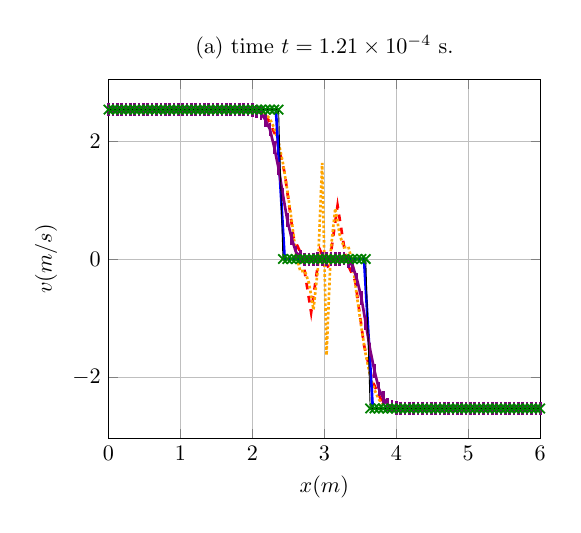
\begin{tikzpicture}[scale=0.8]
\begin{axis}[xlabel=$x (m)$,ylabel=$v (m/s)$,ymajorgrids=true,xmajorgrids=true,legend pos=outer north east,title={(a) time $t = 1.21\times 10^{-4} $ s.},xmin=0.,xmax=6.]
\addplot[Red,very thick,mark=none,dashed,mark size=3pt] coordinates {(0.0,2.5318484177091665) (0.12244897959183673,2.5318484177091665) (0.24489795918367346,2.531848417709166) (0.36734693877551017,2.531848417709166) (0.4897959183673469,2.5318484177091656) (0.6122448979591837,2.5318484177091665) (0.7346938775510203,2.531848417709167) (0.8571428571428571,2.5318484177091665) (0.9795918367346939,2.5318484177091665) (1.1020408163265305,2.5318484177091665) (1.2244897959183674,2.5318484177091665) (1.346938775510204,2.5318484177091665) (1.4693877551020407,2.5318484177091665) (1.5918367346938775,2.5318484177091665) (1.7142857142857142,2.5318484177091665) (1.836734693877551,2.531684227710154) (1.9591836734693877,2.528883339491711) (2.0816326530612246,2.5069977784469075) (2.204081632653061,2.405451093175476) (2.326530612244898,2.0843630627542513) (2.4489795918367347,1.4571958994685654) (2.571428571428571,0.3681332942558399) (2.693877551020408,0.03859430800310576) (2.816326530612245,-0.9060776804312415) (2.9387755102040813,0.15497604259705183) (3.061224489795918,-0.15497604259704956) (3.183673469387755,0.9060776804312402) (3.306122448979592,-0.038594308003106204) (3.4285714285714284,-0.3681332942558391) (3.5510204081632653,-1.4571958994685674) (3.673469387755102,-2.084363062754252) (3.7959183673469385,-2.4054510931754756) (3.9183673469387754,-2.506997778446907) (4.040816326530612,-2.5288833394917107) (4.163265306122449,-2.531684227710154) (4.285714285714286,-2.5318484177091665) (4.408163265306122,-2.5318484177091665) (4.530612244897959,-2.5318484177091665) (4.653061224489796,-2.5318484177091665) (4.775510204081632,-2.5318484177091665) (4.8979591836734695,-2.5318484177091665) (5.020408163265306,-2.5318484177091665) (5.142857142857142,-2.5318484177091665) (5.26530612244898,-2.5318484177091665) (5.387755102040816,-2.5318484177091665) (5.5102040816326525,-2.5318484177091665) (5.63265306122449,-2.5318484177091665) (5.755102040816326,-2.5318484177091665) (5.877551020408163,-2.5318484177091665) (6.0,-2.5318484177091665) };
\addplot[Orange,very thick,mark=none,densely dotted,mark size=3pt] coordinates {(0.0,2.5318484177091665) (0.06060606060606061,2.5318484177091665) (0.12121212121212122,2.5318484177091665) (0.18181818181818182,2.5318484177091665) (0.24242424242424243,2.5318484177091665) (0.30303030303030304,2.5318484177091665) (0.36363636363636365,2.5318484177091665) (0.42424242424242425,2.5318484177091665) (0.48484848484848486,2.5318484177091665) (0.5454545454545454,2.5318484177091665) (0.6060606060606061,2.5318484177091665) (0.6666666666666667,2.531848417709167) (0.7272727272727273,2.531848417709167) (0.7878787878787878,2.5318484177091665) (0.8484848484848485,2.5318484177091665) (0.9090909090909092,2.5318484177091674) (0.9696969696969697,2.5318484177091665) (1.0303030303030303,2.5318484177091665) (1.0909090909090908,2.5318484177091656) (1.1515151515151516,2.5318484177091665) (1.2121212121212122,2.5318484177091665) (1.2727272727272727,2.5318484177091665) (1.3333333333333335,2.5318484177091656) (1.393939393939394,2.531848417709166) (1.4545454545454546,2.5318484177091665) (1.5151515151515151,2.5318484177091656) (1.5757575757575757,2.5318484177091665) (1.6363636363636365,2.531848417709167) (1.696969696969697,2.5318484177091665) (1.7575757575757576,2.5318484177091665) (1.8181818181818183,2.5318020034751854) (1.878787878787879,2.5317091750072236) (1.9393939393939394,2.5307501424302727) (2.0,2.5289249057443333) (2.0606060606060606,2.5201129167796545) (2.121212121212121,2.504314175536237) (2.1818181818181817,2.4573457248537327) (2.2424242424242427,2.379207564732142) (2.303030303030303,2.2185258725100665) (2.3636363636363638,1.975300648187503) (2.4242424242424243,1.625621223269172) (2.484848484848485,1.1694875977550743) (2.5454545454545454,0.6521580355962723) (2.606060606060606,0.07363253679276927) (2.666666666666667,-0.20959340058418097) (2.7272727272727275,-0.1975197765345734) (2.787878787878788,-0.4134073094303823) (2.8484848484848486,-0.8572559992716083) (2.909090909090909,-0.17642315371687442) (2.9696969696969697,1.6290912272338196) (3.0303030303030303,-1.6290912272338194) (3.090909090909091,0.17642315371686795) (3.1515151515151514,0.8572559992716065) (3.2121212121212124,0.41340730943038484) (3.272727272727273,0.19751977653457933) (3.3333333333333335,0.20959340058418124) (3.393939393939394,-0.07363253679276877) (3.4545454545454546,-0.6521580355962722) (3.515151515151515,-1.1694875977550738) (3.5757575757575757,-1.6256212232691716) (3.6363636363636367,-1.9753006481875028) (3.6969696969696972,-2.2185258725100656) (3.757575757575758,-2.3792075647321425) (3.8181818181818183,-2.457345724853733) (3.878787878787879,-2.5043141755362366) (3.9393939393939394,-2.520112916779654) (4.0,-2.528924905744333) (4.0606060606060606,-2.5307501424302727) (4.121212121212121,-2.5317091750072236) (4.181818181818182,-2.531802003475186) (4.242424242424242,-2.5318484177091665) (4.303030303030303,-2.5318484177091665) (4.363636363636363,-2.5318484177091665) (4.424242424242425,-2.5318484177091665) (4.484848484848485,-2.5318484177091665) (4.545454545454546,-2.5318484177091665) (4.606060606060606,-2.5318484177091665) (4.666666666666667,-2.5318484177091665) (4.7272727272727275,-2.5318484177091665) (4.787878787878788,-2.5318484177091665) (4.848484848484849,-2.5318484177091665) (4.909090909090909,-2.5318484177091665) (4.96969696969697,-2.5318484177091665) (5.03030303030303,-2.5318484177091665) (5.090909090909091,-2.5318484177091665) (5.151515151515151,-2.5318484177091665) (5.212121212121212,-2.5318484177091665) (5.2727272727272725,-2.5318484177091665) (5.333333333333334,-2.5318484177091665) (5.3939393939393945,-2.5318484177091665) (5.454545454545455,-2.5318484177091665) (5.515151515151516,-2.5318484177091665) (5.575757575757576,-2.5318484177091665) (5.636363636363637,-2.5318484177091665) (5.696969696969697,-2.5318484177091665) (5.757575757575758,-2.5318484177091665) (5.818181818181818,-2.5318484177091665) (5.878787878787879,-2.5318484177091665) (5.9393939393939394,-2.5318484177091665) (6.0,-2.5318484177091665) };
\addplot[Blue,very thick,mark=none,solid,mark size=3pt] coordinates {(0.0,2.531848417709167) (0.12244897959183673,2.5318484177091656) (0.24489795918367346,2.531848417709166) (0.36734693877551017,2.5318484177091665) (0.4897959183673469,2.531848417709166) (0.6122448979591837,2.531848417709166) (0.7346938775510203,2.531848417709166) (0.8571428571428571,2.531848417709166) (0.9795918367346939,2.531848417709166) (1.1020408163265305,2.531848417709166) (1.2244897959183674,2.5318484177091656) (1.346938775510204,2.531848417709166) (1.4693877551020407,2.531848417709166) (1.5918367346938775,2.5318484177091665) (1.7142857142857142,2.531848417709166) (1.836734693877551,2.531848417709167) (1.9591836734693877,2.5318484177091665) (2.0816326530612246,2.5318484177091665) (2.204081632653061,2.5318484177091665) (2.326530612244898,2.5318484177091665) (2.4489795918367347,0.0) (2.571428571428571,-1.131824441720173e-15) (2.693877551020408,3.772748139067242e-16) (2.816326530612245,-3.944304526105059e-31) (2.9387755102040813,7.545496278134482e-16) (3.061224489795918,-1.131824441720173e-15) (3.183673469387755,3.772748139067241e-16) (3.306122448979592,3.772748139067244e-16) (3.4285714285714284,7.545496278134485e-16) (3.5510204081632653,2.220446049250313e-16) (3.673469387755102,-2.5318484177091665) (3.7959183673469385,-2.531848417709166) (3.9183673469387754,-2.531848417709166) (4.040816326530612,-2.531848417709167) (4.163265306122449,-2.531848417709166) (4.285714285714286,-2.5318484177091656) (4.408163265306122,-2.531848417709167) (4.530612244897959,-2.5318484177091665) (4.653061224489796,-2.531848417709166) (4.775510204081632,-2.531848417709167) (4.8979591836734695,-2.5318484177091665) (5.020408163265306,-2.531848417709167) (5.142857142857142,-2.531848417709167) (5.26530612244898,-2.531848417709167) (5.387755102040816,-2.531848417709167) (5.5102040816326525,-2.531848417709167) (5.63265306122449,-2.5318484177091665) (5.755102040816326,-2.531848417709166) (5.877551020408163,-2.531848417709167) (6.0,-2.5318484177091665) };
\addplot[Purple,very thick,mark=|,solid,mark size=3pt] coordinates {(0.0,2.531848417709166) (0.06060606060606061,2.531848417709166) (0.12121212121212122,2.531848417709166) (0.18181818181818182,2.531848417709166) (0.24242424242424243,2.5318484177091656) (0.30303030303030304,2.5318484177091656) (0.36363636363636365,2.5318484177091656) (0.42424242424242425,2.5318484177091656) (0.48484848484848486,2.5318484177091656) (0.5454545454545454,2.531848417709165) (0.6060606060606061,2.531848417709165) (0.6666666666666667,2.531848417709165) (0.7272727272727273,2.531848417709165) (0.7878787878787878,2.531848417709165) (0.8484848484848485,2.531848417709165) (0.9090909090909092,2.5318484177091647) (0.9696969696969697,2.5318484177091647) (1.0303030303030303,2.5318484177091647) (1.0909090909090908,2.5318484177091647) (1.1515151515151516,2.531848417709165) (1.2121212121212122,2.531848417709165) (1.2727272727272727,2.531848417709165) (1.3333333333333335,2.531848417709165) (1.393939393939394,2.531848417709165) (1.4545454545454546,2.531848417709165) (1.5151515151515151,2.5318484177091656) (1.5757575757575757,2.5318484177091656) (1.6363636363636365,2.531848417709166) (1.696969696969697,2.531848417709166) (1.7575757575757576,2.531848417709166) (1.8181818181818183,2.5317555939571394) (1.878787878787879,2.5315699464530863) (1.9393939393939394,2.529300921403548) (2.0,2.5251960488139282) (2.0606060606060606,2.502983668745643) (2.121212121212121,2.4672568379656363) (2.1818181818181817,2.3558296271378385) (2.2424242424242427,2.199909152499134) (2.303030303030303,1.8955358394101423) (2.3636363636363638,1.5350380403392951) (2.4242424242424243,1.0913569359704094) (2.484848484848485,0.6616953448225573) (2.5454545454545454,0.35041226238060424) (2.606060606060606,0.11398111608931762) (2.666666666666667,0.037623711953108305) (2.7272727272727275,-0.006618739561512254) (2.787878787878788,-0.0024042733543885486) (2.8484848484848486,-0.0017885136987410197) (2.909090909090909,-0.0001900946309221662) (2.9696969696969697,4.075039583706578e-05) (3.0303030303030303,-4.075039583690026e-05) (3.090909090909091,0.000190094630922048) (3.1515151515151514,0.001788513698741276) (3.2121212121212124,0.0024042733543890842) (3.272727272727273,0.006618739561513227) (3.3333333333333335,-0.03762371195310714) (3.393939393939394,-0.11398111608931744) (3.4545454545454546,-0.35041226238060363) (3.515151515151515,-0.6616953448225579) (3.5757575757575757,-1.09135693597041) (3.6363636363636367,-1.535038040339297) (3.6969696969696972,-1.8955358394101425) (3.757575757575758,-2.199909152499135) (3.8181818181818183,-2.3558296271378385) (3.878787878787879,-2.4672568379656363) (3.9393939393939394,-2.502983668745643) (4.0,-2.5251960488139282) (4.0606060606060606,-2.5293009214035473) (4.121212121212121,-2.5315699464530863) (4.181818181818182,-2.5317555939571394) (4.242424242424242,-2.531848417709166) (4.303030303030303,-2.531848417709166) (4.363636363636363,-2.531848417709166) (4.424242424242425,-2.531848417709166) (4.484848484848485,-2.531848417709166) (4.545454545454546,-2.531848417709166) (4.606060606060606,-2.531848417709166) (4.666666666666667,-2.531848417709166) (4.7272727272727275,-2.531848417709166) (4.787878787878788,-2.531848417709166) (4.848484848484849,-2.531848417709166) (4.909090909090909,-2.531848417709166) (4.96969696969697,-2.531848417709166) (5.03030303030303,-2.531848417709166) (5.090909090909091,-2.531848417709166) (5.151515151515151,-2.531848417709166) (5.212121212121212,-2.531848417709166) (5.2727272727272725,-2.531848417709166) (5.333333333333334,-2.531848417709166) (5.3939393939393945,-2.531848417709166) (5.454545454545455,-2.531848417709166) (5.515151515151516,-2.531848417709166) (5.575757575757576,-2.531848417709166) (5.636363636363637,-2.531848417709166) (5.696969696969697,-2.531848417709166) (5.757575757575758,-2.531848417709166) (5.818181818181818,-2.531848417709166) (5.878787878787879,-2.531848417709166) (5.9393939393939394,-2.531848417709166) (6.0,-2.5318484177091665) };
\addplot[Green,thick,mark=x,only marks,mark size=3pt] coordinates {(0.0,2.531848417709166) (0.06060606060606061,2.531848417709166) (0.12121212121212122,2.531848417709166) (0.18181818181818182,2.531848417709166) (0.24242424242424243,2.5318484177091665) (0.30303030303030304,2.5318484177091665) (0.36363636363636365,2.5318484177091656) (0.42424242424242425,2.5318484177091656) (0.48484848484848486,2.5318484177091665) (0.5454545454545454,2.5318484177091665) (0.6060606060606061,2.531848417709165) (0.6666666666666667,2.5318484177091656) (0.7272727272727273,2.531848417709166) (0.7878787878787878,2.531848417709166) (0.8484848484848485,2.5318484177091656) (0.9090909090909092,2.5318484177091656) (0.9696969696969697,2.5318484177091665) (1.0303030303030303,2.5318484177091665) (1.0909090909090908,2.5318484177091647) (1.1515151515151516,2.531848417709165) (1.2121212121212122,2.531848417709166) (1.2727272727272727,2.531848417709166) (1.3333333333333335,2.5318484177091647) (1.393939393939394,2.5318484177091647) (1.4545454545454546,2.5318484177091665) (1.5151515151515151,2.5318484177091665) (1.5757575757575757,2.531848417709166) (1.6363636363636365,2.531848417709166) (1.696969696969697,2.531848417709166) (1.7575757575757576,2.531848417709166) (1.8181818181818183,2.531848417709166) (1.878787878787879,2.531848417709166) (1.9393939393939394,2.531848417709166) (2.0,2.531848417709166) (2.0606060606060606,2.5318484177091656) (2.121212121212121,2.531848417709166) (2.1818181818181817,2.5318484177091665) (2.2424242424242427,2.531848417709166) (2.303030303030303,2.5318484177091665) (2.3636363636363638,2.5318484177091665) (2.4242424242424243,7.771561172376108e-16) (2.484848484848485,-2.1094237467877935e-15) (2.5454545454545454,-2.4980018054065835e-16) (2.606060606060606,-1.0824674490095235e-15) (2.666666666666667,8.52730145933733e-16) (2.7272727272727275,8.332007357698796e-16) (2.787878787878788,-6.636926385046085e-16) (2.8484848484848486,-6.685749910455732e-16) (2.909090909090909,-9.666384036373804e-17) (2.9696969696969697,2.734954664404533e-16) (3.0303030303030303,-9.789796087117351e-17) (3.090909090909091,9.860763805712963e-16) (3.1515151515151514,-5.850647289005321e-16) (3.2121212121212124,-3.585610702627896e-17) (3.272727272727273,8.518216860046792e-17) (3.3333333333333335,-1.2838500279050285e-16) (3.393939393939394,1.7783669840585248e-16) (3.4545454545454546,8.942088536749598e-17) (3.515151515151515,-9.992007221626425e-16) (3.5757575757575757,2.331468351712824e-15) (3.6363636363636367,-2.531848417709166) (3.6969696969696972,-2.5318484177091665) (3.757575757575758,-2.531848417709166) (3.8181818181818183,-2.5318484177091665) (3.878787878787879,-2.531848417709166) (3.9393939393939394,-2.5318484177091665) (4.0,-2.531848417709166) (4.0606060606060606,-2.531848417709166) (4.121212121212121,-2.531848417709166) (4.181818181818182,-2.531848417709166) (4.242424242424242,-2.5318484177091665) (4.303030303030303,-2.531848417709167) (4.363636363636363,-2.531848417709165) (4.424242424242425,-2.531848417709165) (4.484848484848485,-2.5318484177091665) (4.545454545454546,-2.5318484177091665) (4.606060606060606,-2.5318484177091665) (4.666666666666667,-2.5318484177091665) (4.7272727272727275,-2.5318484177091656) (4.787878787878788,-2.531848417709166) (4.848484848484849,-2.531848417709166) (4.909090909090909,-2.5318484177091665) (4.96969696969697,-2.531848417709166) (5.03030303030303,-2.5318484177091665) (5.090909090909091,-2.531848417709166) (5.151515151515151,-2.5318484177091665) (5.212121212121212,-2.531848417709166) (5.2727272727272725,-2.5318484177091665) (5.333333333333334,-2.531848417709166) (5.3939393939393945,-2.5318484177091665) (5.454545454545455,-2.531848417709166) (5.515151515151516,-2.5318484177091665) (5.575757575757576,-2.531848417709166) (5.636363636363637,-2.5318484177091665) (5.696969696969697,-2.531848417709166) (5.757575757575758,-2.5318484177091665) (5.818181818181818,-2.531848417709166) (5.878787878787879,-2.5318484177091665) (5.9393939393939394,-2.5318484177091665) (6.0,-2.5318484177091665) };
\addplot[black,thin,mark=pentagone*,solid,mark size=3pt] coordinates {(0.0,2.5318484177091665) (0.06060606060606061,2.5318484177091665) (0.12121212121212122,2.5318484177091665) (0.18181818181818182,2.5318484177091665) (0.24242424242424243,2.5318484177091665) (0.30303030303030304,2.5318484177091665) (0.36363636363636365,2.5318484177091665) (0.42424242424242425,2.5318484177091665) (0.48484848484848486,2.5318484177091665) (0.5454545454545454,2.5318484177091665) (0.6060606060606061,2.5318484177091665) (0.6666666666666667,2.5318484177091665) (0.7272727272727273,2.5318484177091665) (0.7878787878787878,2.5318484177091665) (0.8484848484848485,2.5318484177091665) (0.9090909090909092,2.5318484177091665) (0.9696969696969697,2.5318484177091665) (1.0303030303030303,2.5318484177091665) (1.0909090909090908,2.5318484177091665) (1.1515151515151516,2.5318484177091665) (1.2121212121212122,2.5318484177091665) (1.2727272727272727,2.5318484177091665) (1.3333333333333335,2.5318484177091665) (1.393939393939394,2.5318484177091665) (1.4545454545454546,2.5318484177091665) (1.5151515151515151,2.5318484177091665) (1.5757575757575757,2.5318484177091665) (1.6363636363636365,2.5318484177091665) (1.696969696969697,2.5318484177091665) (1.7575757575757576,2.5318484177091665) (1.8181818181818183,2.5318484177091665) (1.878787878787879,2.5318484177091665) (1.9393939393939394,2.5318484177091665) (2.0,2.5318484177091665) (2.0606060606060606,2.5318484177091665) (2.121212121212121,2.5318484177091665) (2.1818181818181817,2.5318484177091665) (2.2424242424242427,2.5318484177091665) (2.303030303030303,2.5318484177091665) (2.3636363636363638,2.5318484177091665) (2.4242424242424243,0.0) (2.484848484848485,0.0) (2.5454545454545454,0.0) (2.606060606060606,0.0) (2.666666666666667,0.0) (2.7272727272727275,0.0) (2.787878787878788,0.0) (2.8484848484848486,0.0) (2.909090909090909,0.0) (2.9696969696969697,0.0) (3.0303030303030303,-0.0) (3.090909090909091,-0.0) (3.1515151515151514,-0.0) (3.2121212121212124,-0.0) (3.272727272727273,-0.0) (3.3333333333333335,-0.0) (3.393939393939394,-0.0) (3.4545454545454546,-0.0) (3.515151515151515,-0.0) (3.5757575757575757,-0.0) (3.6363636363636367,-2.5318484177091665) (3.6969696969696972,-2.5318484177091665) (3.757575757575758,-2.5318484177091665) (3.8181818181818183,-2.5318484177091665) (3.878787878787879,-2.5318484177091665) (3.9393939393939394,-2.5318484177091665) (4.0,-2.5318484177091665) (4.0606060606060606,-2.5318484177091665) (4.121212121212121,-2.5318484177091665) (4.181818181818182,-2.5318484177091665) (4.242424242424242,-2.5318484177091665) (4.303030303030303,-2.5318484177091665) (4.363636363636363,-2.5318484177091665) (4.424242424242425,-2.5318484177091665) (4.484848484848485,-2.5318484177091665) (4.545454545454546,-2.5318484177091665) (4.606060606060606,-2.5318484177091665) (4.666666666666667,-2.5318484177091665) (4.7272727272727275,-2.5318484177091665) (4.787878787878788,-2.5318484177091665) (4.848484848484849,-2.5318484177091665) (4.909090909090909,-2.5318484177091665) (4.96969696969697,-2.5318484177091665) (5.03030303030303,-2.5318484177091665) (5.090909090909091,-2.5318484177091665) (5.151515151515151,-2.5318484177091665) (5.212121212121212,-2.5318484177091665) (5.2727272727272725,-2.5318484177091665) (5.333333333333334,-2.5318484177091665) (5.3939393939393945,-2.5318484177091665) (5.454545454545455,-2.5318484177091665) (5.515151515151516,-2.5318484177091665) (5.575757575757576,-2.5318484177091665) (5.636363636363637,-2.5318484177091665) (5.696969696969697,-2.5318484177091665) (5.757575757575758,-2.5318484177091665) (5.818181818181818,-2.5318484177091665) (5.878787878787879,-2.5318484177091665) (5.9393939393939394,-2.5318484177091665) (6.0,-2.5318484177091665) };
%\legend{usl 1ppc,usl 2ppc,dgmpm 1ppc,dgmpm 2ppc,dgmpm 2ppc (RK2),exact}
\end{axis}
\end{tikzpicture}
%%% Local Variables:
%%% mode: latex
%%% TeX-master: "../../mainManuscript"
%%% End:
}
  {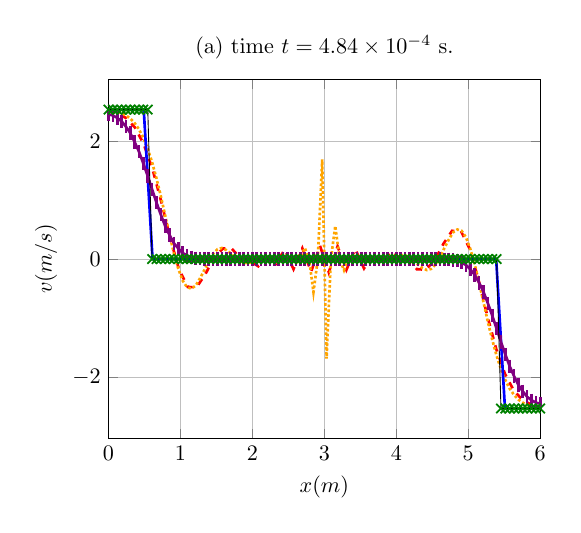
\begin{tikzpicture}[scale=0.8]
\begin{axis}[xlabel=$x (m)$,ylabel=$v (m/s)$,ymajorgrids=true,xmajorgrids=true,legend pos=outer north east,title={(a) time $t = 4.84\times 10^{-4} $ s.},xmin=0.,xmax=6.]
\addplot[Red,very thick,mark=none,dashed,mark size=3pt] coordinates {(0.0,2.5010841927729737) (0.12244897959183673,2.469190114266878) (0.24489795918367346,2.388524326251144) (0.36734693877551017,2.2273018421403252) (0.4897959183673469,1.9469489967062041) (0.6122448979591837,1.5210982531835537) (0.7346938775510203,0.9639084261801771) (0.8571428571428571,0.35350426741421853) (0.9795918367346939,-0.17346522218220087) (1.1020408163265305,-0.4738949800515782) (1.2244897959183674,-0.4781129013135259) (1.346938775510204,-0.2546047420872028) (1.4693877551020407,0.03038529149069727) (1.5918367346938775,0.17867317133486063) (1.7142857142857142,0.17318519647638472) (1.836734693877551,0.009715941997365168) (1.9591836734693877,-0.02832074608631413) (2.0816326530612246,-0.1225397720856652) (2.204081632653061,0.0701451861529502) (2.326530612244898,-0.07977872830116252) (2.4489795918367347,0.1588281886075272) (2.571428571428571,-0.1717009307352768) (2.693877551020408,0.18355506260116172) (2.816326530612245,-0.2148933313216084) (2.9387755102040813,0.22532520111024354) (3.061224489795918,-0.2253252011102409) (3.183673469387755,0.2148933313216084) (3.306122448979592,-0.18355506260115909) (3.4285714285714284,0.17170093073527581) (3.5510204081632653,-0.1588281886075268) (3.673469387755102,0.07977872830116275) (3.7959183673469385,-0.0701451861529482) (3.9183673469387754,0.12253977208566608) (4.040816326530612,0.028320746086314623) (4.163265306122449,-0.009715941997368367) (4.285714285714286,-0.17318519647638597) (4.408163265306122,-0.17867317133486066) (4.530612244897959,-0.03038529149069498) (4.653061224489796,0.2546047420872032) (4.775510204081632,0.47811290131352563) (4.8979591836734695,0.47389498005157743) (5.020408163265306,0.17346522218220176) (5.142857142857142,-0.35350426741421775) (5.26530612244898,-0.9639084261801814) (5.387755102040816,-1.5210982531835537) (5.5102040816326525,-1.9469489967062041) (5.63265306122449,-2.2273018421403257) (5.755102040816326,-2.388524326251146) (5.877551020408163,-2.469190114266878) (6.0,-2.501084192772974) };
\addplot[Orange,very thick,mark=none,densely dotted,mark size=3pt] coordinates {(0.0,2.512922289601415) (0.06060606060606061,2.507159803666336) (0.12121212121212122,2.4933072053261904) (0.18181818181818182,2.4713644945809774) (0.24242424242424243,2.4341811221412843) (0.30303030303030304,2.381757088007112) (0.36363636363636365,2.302584217587779) (0.42424242424242425,2.1966625108832853) (0.48484848484848486,2.051636723745046) (0.5454545454545454,1.8675068561730643) (0.6060606060606061,1.6395141655892098) (0.6666666666666667,1.367658651993486) (0.7272727272727273,1.0659200652949896) (0.7878787878787878,0.7342984054937217) (0.8484848484848485,0.4105666475914286) (0.9090909090909092,0.09472479158810959) (0.9696969696969697,-0.16372314354382467) (1.0303030303030303,-0.3647771578043735) (1.0909090909090908,-0.47704489390672733) (1.1515151515151516,-0.5005263518508837) (1.2121212121212122,-0.4498657239486042) (1.2727272727272727,-0.32506301019988637) (1.3333333333333335,-0.18348993400450103) (1.393939393939394,-0.02514649536244179) (1.4545454545454546,0.09159748054237633) (1.5151515151515151,0.16674199370995474) (1.5757575757575757,0.18691089986382955) (1.6363636363636365,0.1521041990039989) (1.696969696969697,0.0975148523025528) (1.7575757575757576,0.023142859759495475) (1.8181818181818183,-0.030403372776003856) (1.878787878787879,-0.06312384530394177) (1.9393939393939394,-0.06886040223069545) (2.0,-0.04761304355625976) (2.0606060606060606,-0.023072733446745507) (2.121212121212121,0.004760528097847733) (2.1818181818181817,0.021185203676438287) (2.2424242424242427,0.026201293289025814) (2.303030303030303,0.018938648459264136) (2.3636363636363638,-0.0006027308128485212) (2.4242424242424243,-0.0025695183595292256) (2.484848484848485,0.013038285819222022) (2.5454545454545454,-0.00841329842817132) (2.606060606060606,-0.06692427110170765) (2.666666666666667,-0.0009936080373927803) (2.7272727272727275,0.1893786907647767) (2.787878787878788,0.0028453568328217853) (2.8484848484848486,-0.5605936098332589) (2.909090909090909,0.0012272845525674915) (2.9696969696969697,1.6883080399903014) (3.0303030303030303,-1.6883080399902968) (3.090909090909091,-0.001227284552569761) (3.1515151515151514,0.5605936098332589) (3.2121212121212124,-0.002845356832822726) (3.272727272727273,-0.1893786907647747) (3.3333333333333335,0.0009936080373919875) (3.393939393939394,0.06692427110170816) (3.4545454545454546,0.008413298428171269) (3.515151515151515,-0.01303828581922206) (3.5757575757575757,0.0025695183595286896) (3.6363636363636367,0.0006027308128476435) (3.6969696969696972,-0.018938648459265153) (3.757575757575758,-0.02620129328902751) (3.8181818181818183,-0.02118520367643984) (3.878787878787879,-0.004760528097848594) (3.9393939393939394,0.023072733446745295) (4.0,0.04761304355625988) (4.0606060606060606,0.06886040223069606) (4.121212121212121,0.06312384530394438) (4.181818181818182,0.03040337277600426) (4.242424242424242,-0.023142859759493872) (4.303030303030303,-0.09751485230255147) (4.363636363636363,-0.15210419900399794) (4.424242424242425,-0.18691089986382994) (4.484848484848485,-0.16674199370995568) (4.545454545454546,-0.09159748054237618) (4.606060606060606,0.025146495362441262) (4.666666666666667,0.1834899340044987) (4.7272727272727275,0.32506301019988665) (4.787878787878788,0.44986572394860463) (4.848484848484849,0.5005263518508843) (4.909090909090909,0.4770448939067263) (4.96969696969697,0.3647771578043749) (5.03030303030303,0.1637231435438261) (5.090909090909091,-0.09472479158810942) (5.151515151515151,-0.4105666475914277) (5.212121212121212,-0.7342984054937214) (5.2727272727272725,-1.0659200652949885) (5.333333333333334,-1.3676586519934855) (5.3939393939393945,-1.6395141655892107) (5.454545454545455,-1.867506856173064) (5.515151515151516,-2.051636723745046) (5.575757575757576,-2.1966625108832845) (5.636363636363637,-2.3025842175877775) (5.696969696969697,-2.3817570880071117) (5.757575757575758,-2.4341811221412852) (5.818181818181818,-2.4713644945809774) (5.878787878787879,-2.4933072053261904) (5.9393939393939394,-2.5071598036663363) (6.0,-2.512922289601414) };
\addplot[Blue,very thick,mark=none,solid,mark size=3pt] coordinates {(0.0,2.531848417709166) (0.12244897959183673,2.531848417709167) (0.24489795918367346,2.531848417709167) (0.36734693877551017,2.531848417709165) (0.4897959183673469,2.5318484177091647) (0.6122448979591837,-6.661338147750939e-16) (0.7346938775510203,-2.242047466345328e-15) (0.8571428571428571,-1.336287918866768e-16) (0.9795918367346939,1.3990820254935266e-15) (1.1020408163265305,-1.7763568394002503e-15) (1.2244897959183674,-3.240243116178825e-15) (1.346938775510204,2.841366885177086e-15) (1.4693877551020407,-1.3538690466452047e-15) (1.5918367346938775,-3.772748139067242e-16) (1.7142857142857142,-5.993194188317551e-16) (1.836734693877551,2.3520646964787014e-15) (1.9591836734693877,9.097798367951425e-16) (2.0816326530612246,2.9513841153104565e-15) (2.204081632653061,-1.886374069533622e-15) (2.326530612244898,1.5090992556268973e-15) (2.4489795918367347,-3.772748139067235e-16) (2.571428571428571,1.1318244417201719e-15) (2.693877551020408,-1.1318244417201734e-15) (2.816326530612245,1.886374069533621e-15) (2.9387755102040813,-3.0181985112537953e-15) (3.061224489795918,1.509099255626895e-15) (3.183673469387755,-3.3954733251605203e-15) (3.306122448979592,1.131824441720175e-15) (3.4285714285714284,-7.54549627813448e-16) (3.5510204081632653,2.2204460492503017e-16) (3.673469387755102,-1.7527452776469433e-15) (3.7959183673469385,1.819559673590282e-15) (3.9183673469387754,1.3362879188667458e-16) (4.040816326530612,-1.5759136515702374e-15) (4.163265306122449,-7.997626066617703e-16) (4.285714285714286,-4.521297884831934e-17) (4.408163265306122,-3.906376930953917e-15) (4.530612244897959,3.79434955616226e-15) (4.653061224489796,-3.861163952105597e-15) (4.775510204081632,1.6643294646085906e-15) (4.8979591836734695,-4.1068201187839345e-15) (5.020408163265306,6.209208359267724e-16) (5.142857142857142,-2.7745524892337463e-15) (5.26530612244898,9.98195649833496e-16) (5.387755102040816,-6.661338147750939e-16) (5.5102040816326525,-2.531848417709167) (5.63265306122449,-2.531848417709165) (5.755102040816326,-2.531848417709168) (5.877551020408163,-2.531848417709166) (6.0,-2.531848417709165) };
\addplot[Purple,very thick,mark=|,solid,mark size=3pt] coordinates {(0.0,2.4502878879638077) (0.06060606060606061,2.4331156617141234) (0.12121212121212122,2.3912249841562767) (0.18181818181818182,2.334329048267753) (0.24242424242424243,2.2418909444576474) (0.30303030303030304,2.133656683027458) (0.36363636363636365,1.982993211922006) (0.42424242424242425,1.8174087611146408) (0.48484848484848486,1.6154775867478133) (0.5454545454545454,1.4047401021710633) (0.6060606060606061,1.1801065385155256) (0.6666666666666667,0.9574083982688202) (0.7272727272727273,0.7516285480780078) (0.7878787878787878,0.5581100772293209) (0.8484848484848485,0.40510029277008563) (0.9090909090909092,0.2688057300718126) (0.9696969696969697,0.1784269686067307) (1.0303030303030303,0.10222920629772528) (1.0909090909090908,0.06123973598946104) (1.1515151515151516,0.028491831319577256) (1.2121212121212122,0.015077503968816922) (1.2727272727272727,0.004852500743675085) (1.3333333333333335,0.002132768618835191) (1.393939393939394,9.497890449658636e-05) (1.4545454545454546,-3.613906028997789e-05) (1.5151515151515151,-0.0001771883066314252) (1.5757575757575757,-8.197840812272274e-05) (1.6363636363636365,-3.778569739159183e-05) (1.696969696969697,-1.3168311989532245e-05) (1.7575757575757576,-7.18048230077542e-07) (1.8181818181818183,1.2525161562481774e-07) (1.878787878787879,7.57143015280698e-07) (1.9393939393939394,2.448660220997095e-07) (2.0,7.135513801818636e-08) (2.0606060606060606,1.4595492827506847e-08) (2.121212121212121,-6.363153796720189e-09) (2.1818181818181817,-1.8377351508576813e-09) (2.2424242424242427,-9.025903498190151e-10) (2.303030303030303,-1.5217965502392056e-10) (2.3636363636363638,3.1015363059108134e-11) (2.4242424242424243,7.240747155190924e-12) (2.484848484848485,4.49718045151787e-12) (2.5454545454545454,4.994640475976035e-13) (2.606060606060606,-1.0901286833703581e-13) (2.666666666666667,-1.5949332804559343e-14) (2.7272727272727275,-8.856384153319333e-15) (2.787878787878788,-1.6410925375832847e-15) (2.8484848484848486,-6.505398960621357e-16) (2.909090909090909,-1.0083526676638663e-15) (2.9696969696969697,-1.001626558081926e-15) (3.0303030303030303,-8.578917651911006e-16) (3.090909090909091,-8.575534244519106e-16) (3.1515151515151514,-5.996684329169147e-16) (3.2121212121212124,-8.861306261599516e-17) (3.272727272727273,6.792476193910383e-15) (3.3333333333333335,1.3748077565965016e-14) (3.393939393939394,1.0666160267206766e-13) (3.4545454545454546,-5.017226512299146e-13) (3.515151515151515,-4.499410687924808e-12) (3.5757575757575757,-7.243247705404374e-12) (3.6363636363636367,-3.1017486754894407e-11) (3.6969696969696972,1.5217809344571135e-10) (3.757575757575758,9.025888787161362e-10) (3.8181818181818183,1.8377338911614902e-09) (3.878787878787879,6.363153398776474e-09) (3.9393939393939394,-1.4595492913112185e-08) (4.0,-7.135513834340724e-08) (4.0606060606060606,-2.4486602290663936e-07) (4.121212121212121,-7.571430163470533e-07) (4.181818181818182,-1.252516171290449e-07) (4.242424242424242,7.180482286441556e-07) (4.303030303030303,1.3168311988130426e-05) (4.363636363636363,3.7785697390737625e-05) (4.424242424242425,8.197840812161226e-05) (4.484848484848485,0.00017718830662956148) (4.545454545454546,3.613906028778548e-05) (4.606060606060606,-9.497890449961183e-05) (4.666666666666667,-0.002132768618838574) (4.7272727272727275,-0.00485250074367774) (4.787878787878788,-0.015077503968819619) (4.848484848484849,-0.02849183131958028) (4.909090909090909,-0.0612397359894635) (4.96969696969697,-0.10222920629772878) (5.03030303030303,-0.17842696860673407) (5.090909090909091,-0.2688057300718156) (5.151515151515151,-0.40510029277008763) (5.212121212121212,-0.5581100772293224) (5.2727272727272725,-0.7516285480780089) (5.333333333333334,-0.9574083982688223) (5.3939393939393945,-1.1801065385155272) (5.454545454545455,-1.4047401021710655) (5.515151515151516,-1.6154775867478157) (5.575757575757576,-1.8174087611146434) (5.636363636363637,-1.982993211922008) (5.696969696969697,-2.1336566830274606) (5.757575757575758,-2.2418909444576505) (5.818181818181818,-2.3343290482677563) (5.878787878787879,-2.39122498415628) (5.9393939393939394,-2.433115661714126) (6.0,-2.4502878879638113) };
\addplot[Green,thick,mark=x,only marks,mark size=3pt] coordinates {(0.0,2.5318484177091647) (0.06060606060606061,2.5318484177091647) (0.12121212121212122,2.5318484177091642) (0.18181818181818182,2.5318484177091642) (0.24242424242424243,2.5318484177091625) (0.30303030303030304,2.5318484177091625) (0.36363636363636365,2.531848417709162) (0.42424242424242425,2.5318484177091616) (0.48484848484848486,2.5318484177091647) (0.5454545454545454,2.5318484177091647) (0.6060606060606061,-2.5535129566378593e-15) (0.6666666666666667,-4.107825191113079e-15) (0.7272727272727273,-1.1821865067599611e-15) (0.7878787878787878,-1.0382595424903476e-15) (0.8484848484848485,-2.594083204450083e-16) (0.9090909090909092,-5.423644308750513e-16) (0.9696969696969697,-2.7327311521224373e-15) (1.0303030303030303,-2.729968157964989e-15) (1.0909090909090908,-1.849588141779186e-15) (1.1515151515151516,-2.591303956721436e-15) (1.2121212121212122,3.2358887055886763e-16) (1.2727272727272727,-4.140148282555056e-16) (1.3333333333333335,-2.964668530546082e-15) (1.393939393939394,-2.985322823581436e-15) (1.4545454545454546,-3.431128126883216e-16) (1.5151515151515151,-3.6823398093509377e-16) (1.5757575757575757,-4.976978604008548e-16) (1.6363636363636365,-7.913669349592946e-16) (1.696969696969697,9.30104610666006e-16) (1.7575757575757576,1.781082693008645e-16) (1.8181818181818183,-3.200542091552869e-16) (1.878787878787879,-2.57663792581449e-16) (1.9393939393939394,-1.066037019433047e-16) (2.0,-2.7025089943367067e-17) (2.0606060606060606,-1.393229467111157e-15) (2.121212121212121,-5.16756164175769e-16) (2.1818181818181817,-4.3607449790516604e-16) (2.2424242424242427,-3.184751299082477e-16) (2.303030303030303,4.580155256428032e-16) (2.3636363636363638,9.174549380974228e-16) (2.4242424242424243,-1.6015820734760246e-15) (2.484848484848485,-4.852351838876055e-16) (2.5454545454545454,-4.2783451322396646e-17) (2.606060606060606,2.1961507739911167e-16) (2.666666666666667,-2.13962396391271e-15) (2.7272727272727275,-2.210842176891267e-15) (2.787878787878788,5.451677388715817e-16) (2.8484848484848486,3.862135150185818e-16) (2.909090909090909,-1.0581116162267363e-15) (2.9696969696969697,-1.0287056411368938e-15) (3.0303030303030303,2.4107097344619627e-16) (3.090909090909091,-1.0744218155952165e-16) (3.1515151515151514,3.612033351810279e-16) (3.2121212121212124,5.269750845190583e-16) (3.272727272727273,-9.56438222610769e-16) (3.3333333333333335,-5.958638672061637e-16) (3.393939393939394,9.031576787357558e-16) (3.4545454545454546,8.731991606644893e-16) (3.515151515151515,-4.649512583958853e-16) (3.5757575757575757,-4.664299954942793e-16) (3.6363636363636367,-2.658188422087487e-16) (3.6969696969696972,8.898721613203251e-17) (3.757575757575758,9.018038775143556e-16) (3.8181818181818183,4.3046375203582656e-16) (3.878787878787879,-2.006864452247978e-15) (3.9393939393939394,-2.386804522746043e-15) (4.0,2.916840469072776e-16) (4.0606060606060606,5.964943727928409e-16) (4.121212121212121,4.3783343187558093e-16) (4.181818181818182,8.94434197674601e-16) (4.242424242424242,-7.57073748850323e-16) (4.303030303030303,-4.067871315316464e-17) (4.363636363636363,5.414274681889935e-16) (4.424242424242425,6.140085352842909e-16) (4.484848484848485,-1.2141910461027111e-15) (4.545454545454546,-1.4031210894910502e-15) (4.606060606060606,-1.6965880323555225e-16) (4.666666666666667,-8.95351242541286e-16) (4.7272727272727275,1.334674378172877e-15) (4.787878787878788,4.41682461227368e-16) (4.848484848484849,-1.0242381251598384e-15) (4.909090909090909,-1.4162423843572238e-15) (4.96969696969697,1.3047396462906642e-15) (5.03030303030303,9.157064029596423e-16) (5.090909090909091,-8.666079337415476e-16) (5.151515151515151,-8.193229479620654e-16) (5.212121212121212,-3.2176366267546826e-16) (5.2727272727272725,-2.991571732513092e-16) (5.333333333333334,-6.661338147750951e-16) (5.3939393939393945,2.44249065417534e-15) (5.454545454545455,-2.531848417709165) (5.515151515151516,-2.531848417709165) (5.575757575757576,-2.5318484177091656) (5.636363636363637,-2.531848417709166) (5.696969696969697,-2.531848417709165) (5.757575757575758,-2.5318484177091656) (5.818181818181818,-2.531848417709166) (5.878787878787879,-2.531848417709166) (5.9393939393939394,-2.5318484177091656) (6.0,-2.5318484177091656) };
\addplot[black,thin,mark=pentagone*,solid,mark size=3pt] coordinates {(0.0,2.5318484177091665) (0.06060606060606061,2.5318484177091665) (0.12121212121212122,2.5318484177091665) (0.18181818181818182,2.5318484177091665) (0.24242424242424243,2.5318484177091665) (0.30303030303030304,2.5318484177091665) (0.36363636363636365,2.5318484177091665) (0.42424242424242425,2.5318484177091665) (0.48484848484848486,2.5318484177091665) (0.5454545454545454,2.5318484177091665) (0.6060606060606061,0.0) (0.6666666666666667,0.0) (0.7272727272727273,0.0) (0.7878787878787878,0.0) (0.8484848484848485,0.0) (0.9090909090909092,0.0) (0.9696969696969697,0.0) (1.0303030303030303,0.0) (1.0909090909090908,0.0) (1.1515151515151516,0.0) (1.2121212121212122,0.0) (1.2727272727272727,0.0) (1.3333333333333335,0.0) (1.393939393939394,0.0) (1.4545454545454546,0.0) (1.5151515151515151,0.0) (1.5757575757575757,0.0) (1.6363636363636365,0.0) (1.696969696969697,0.0) (1.7575757575757576,0.0) (1.8181818181818183,0.0) (1.878787878787879,0.0) (1.9393939393939394,0.0) (2.0,0.0) (2.0606060606060606,0.0) (2.121212121212121,0.0) (2.1818181818181817,0.0) (2.2424242424242427,0.0) (2.303030303030303,0.0) (2.3636363636363638,0.0) (2.4242424242424243,0.0) (2.484848484848485,0.0) (2.5454545454545454,0.0) (2.606060606060606,0.0) (2.666666666666667,0.0) (2.7272727272727275,0.0) (2.787878787878788,0.0) (2.8484848484848486,0.0) (2.909090909090909,0.0) (2.9696969696969697,0.0) (3.0303030303030303,-0.0) (3.090909090909091,-0.0) (3.1515151515151514,-0.0) (3.2121212121212124,-0.0) (3.272727272727273,-0.0) (3.3333333333333335,-0.0) (3.393939393939394,-0.0) (3.4545454545454546,-0.0) (3.515151515151515,-0.0) (3.5757575757575757,-0.0) (3.6363636363636367,-0.0) (3.6969696969696972,-0.0) (3.757575757575758,-0.0) (3.8181818181818183,-0.0) (3.878787878787879,-0.0) (3.9393939393939394,-0.0) (4.0,-0.0) (4.0606060606060606,-0.0) (4.121212121212121,-0.0) (4.181818181818182,-0.0) (4.242424242424242,-0.0) (4.303030303030303,-0.0) (4.363636363636363,-0.0) (4.424242424242425,-0.0) (4.484848484848485,-0.0) (4.545454545454546,-0.0) (4.606060606060606,-0.0) (4.666666666666667,-0.0) (4.7272727272727275,-0.0) (4.787878787878788,-0.0) (4.848484848484849,-0.0) (4.909090909090909,-0.0) (4.96969696969697,-0.0) (5.03030303030303,-0.0) (5.090909090909091,-0.0) (5.151515151515151,-0.0) (5.212121212121212,-0.0) (5.2727272727272725,-0.0) (5.333333333333334,-0.0) (5.3939393939393945,-0.0) (5.454545454545455,-2.5318484177091665) (5.515151515151516,-2.5318484177091665) (5.575757575757576,-2.5318484177091665) (5.636363636363637,-2.5318484177091665) (5.696969696969697,-2.5318484177091665) (5.757575757575758,-2.5318484177091665) (5.818181818181818,-2.5318484177091665) (5.878787878787879,-2.5318484177091665) (5.9393939393939394,-2.5318484177091665) (6.0,-2.5318484177091665) };
%\legend{usl 1ppc,usl 2ppc,dgmpm 1ppc,dgmpm 2ppc,dgmpm 2ppc (RK2),exact}
\end{axis}
\end{tikzpicture}
%%% Local Variables:
%%% mode: latex
%%% TeX-master: "../../mainManuscript"
%%% End:
}
 \caption{elastic RP velo}
  \label{fig:velo_elastic_RP}
\end{figure}


\subsection{Elastoviscoplastic material}


\subsection{Elastoplastic material}
Comparison with mpm for 1ppc
\begin{figure}[h!]
  \centering
  {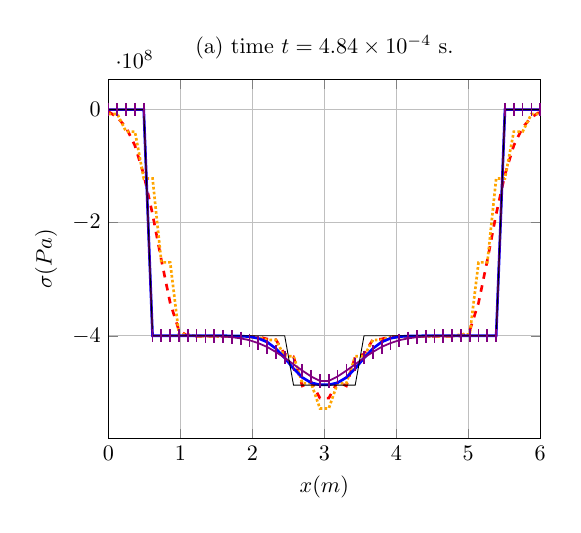
\begin{tikzpicture}[scale=0.8]
\begin{axis}[xlabel=$x (m)$,ylabel=$\sigma (Pa)$,ymajorgrids=true,xmajorgrids=true,legend pos=outer north east,title={(a) time $t = 4.84\times 10^{-4} $ s.},xmin=0.,xmax=6.]
\addplot[Red,very thick,mark=none,dashed,mark size=3pt] coordinates {(0.0,-3669561.908091424) (0.12244897959183673,-13594450.379485756) (0.24489795918367346,-31624435.10565728) (0.36734693877551017,-63707048.32128755) (0.4897959183673469,-114660806.5675256) (0.6122448979591837,-184794660.6509606) (0.7346938775510203,-266179173.63903272) (0.8571428571428571,-341775310.1478163) (0.9795918367346939,-390693099.4776282) (1.1020408163265305,-400379159.02115166) (1.2244897959183674,-400770866.2752631) (1.346938775510204,-400849758.67078286) (1.4693877551020407,-400903087.2437715) (1.5918367346938775,-400974206.0457186) (1.7142857142857142,-401177729.4632526) (1.836734693877551,-401187799.71208847) (1.9591836734693877,-401722959.3911894) (2.0816326530612246,-401625095.9277148) (2.204081632653061,-405721718.460188) (2.326530612244898,-406980928.2270958) (2.4489795918367347,-432556847.70391244) (2.571428571428571,-437038541.50331527) (2.693877551020408,-488555362.3021708) (2.816326530612245,-481341619.82050365) (2.9387755102040813,-510307309.7388937) (3.061224489795918,-510307309.7388923) (3.183673469387755,-481341619.8205054) (3.306122448979592,-488555362.3021694) (3.4285714285714284,-437038541.50331557) (3.5510204081632653,-432556847.70391184) (3.673469387755102,-406980928.2270957) (3.7959183673469385,-405721718.4601879) (3.9183673469387754,-401625095.9277147) (4.040816326530612,-401722959.3911895) (4.163265306122449,-401187799.71208847) (4.285714285714286,-401177729.4632526) (4.408163265306122,-400974206.0457186) (4.530612244897959,-400903087.2437715) (4.653061224489796,-400849758.670783) (4.775510204081632,-400770866.2752632) (4.8979591836734695,-400379159.02115154) (5.020408163265306,-390693099.47762805) (5.142857142857142,-341775310.1478161) (5.26530612244898,-266179173.63903314) (5.387755102040816,-184794660.65096068) (5.5102040816326525,-114660806.56752594) (5.63265306122449,-63707048.32128816) (5.755102040816326,-31624435.10565742) (5.877551020408163,-13594450.3794861) (6.0,-3669561.9080915614) };
\addplot[Orange,very thick,mark=none,densely dotted,mark size=3pt] coordinates {(0.0,-7704082.21541914) (0.12244897959183673,-7704082.215419964) (0.24489795918367346,-38910767.179807946) (0.36734693877551017,-38910767.179809734) (0.4897959183673469,-121706082.18231319) (0.6122448979591837,-121706082.18231393) (0.7346938775510203,-270178420.86149406) (0.8571428571428571,-270178420.86149424) (0.9795918367346939,-397531432.1356541) (1.1020408163265305,-397531432.1356535) (1.2244897959183674,-401012534.0605535) (1.346938775510204,-401012534.06055355) (1.4693877551020407,-401234952.7304736) (1.5918367346938775,-401234952.7304736) (1.7142857142857142,-401510249.2649837) (1.836734693877551,-401510249.26498365) (1.9591836734693877,-402468617.2069635) (2.0816326530612246,-402468617.20696384) (2.204081632653061,-407504349.4174507) (2.326530612244898,-407504349.41745126) (2.4489795918367347,-436281593.4206602) (2.571428571428571,-436281593.4206595) (2.693877551020408,-483800764.100225) (2.816326530612245,-483800764.1002225) (2.9387755102040813,-528538483.5810668) (3.061224489795918,-528538483.5810619) (3.183673469387755,-483800764.1002253) (3.306122448979592,-483800764.1002222) (3.4285714285714284,-436281593.4206605) (3.5510204081632653,-436281593.4206591) (3.673469387755102,-407504349.4174511) (3.7959183673469385,-407504349.4174508) (3.9183673469387754,-402468617.2069634) (4.040816326530612,-402468617.2069638) (4.163265306122449,-401510249.2649835) (4.285714285714286,-401510249.2649837) (4.408163265306122,-401234952.7304736) (4.530612244897959,-401234952.73047346) (4.653061224489796,-401012534.0605535) (4.775510204081632,-401012534.06055355) (4.8979591836734695,-397531432.1356546) (5.020408163265306,-397531432.1356539) (5.142857142857142,-270178420.8614938) (5.26530612244898,-270178420.8614949) (5.387755102040816,-121706082.18231441) (5.5102040816326525,-121706082.18231332) (5.63265306122449,-38910767.17980904) (5.755102040816326,-38910767.1798085) (5.877551020408163,-7704082.215420583) (6.0,-7704082.215419208) };
\addplot[Blue,very thick,mark=none,solid,mark size=3pt] coordinates {(0.0,-1.4032094709741823e-07) (0.12244897959183673,1.4032094709741797e-07) (0.24489795918367346,-5.501313561848306e-23) (0.36734693877551017,-1.4032094709741882e-07) (0.4897959183673469,-4.2096284129225576e-07) (0.6122448979591837,-400000000.0000052) (0.7346938775510203,-400000000.0003803) (0.8571428571428571,-400000000.0131417) (0.9795918367346939,-400000000.2874559) (1.1020408163265305,-400000004.46415013) (1.2244897959183674,-400000052.34678423) (1.346938775510204,-400000481.2046858) (1.4693877551020407,-400003554.03647596) (1.5918367346938775,-400021443.0967657) (1.7142857142857142,-400106894.9802318) (1.836734693877551,-400443646.6051052) (1.9591836734693877,-401540408.59283984) (2.0816326530612246,-404487333.2231472) (2.204081632653061,-410984305.87262785) (2.326530612244898,-422622254.02503896) (2.4489795918367347,-439299786.1010327) (2.571428571428571,-457971198.93456453) (2.693877551020408,-473710434.18348145) (2.816326530612245,-483108267.7934754) (2.9387755102040813,-486652315.1909913) (3.061224489795918,-486652315.1909913) (3.183673469387755,-483108267.7934754) (3.306122448979592,-473710434.18348145) (3.4285714285714284,-457971198.93456453) (3.5510204081632653,-439299786.1010328) (3.673469387755102,-422622254.025039) (3.7959183673469385,-410984305.8726279) (3.9183673469387754,-404487333.2231472) (4.040816326530612,-401540408.59283984) (4.163265306122449,-400443646.6051051) (4.285714285714286,-400106894.98023176) (4.408163265306122,-400021443.0967656) (4.530612244897959,-400003554.0364758) (4.653061224489796,-400000481.20468575) (4.775510204081632,-400000052.3467841) (4.8979591836734695,-400000004.46415013) (5.020408163265306,-400000000.2874559) (5.142857142857142,-400000000.01314175) (5.26530612244898,-400000000.0003803) (5.387755102040816,-400000000.0000052) (5.5102040816326525,1.403209470974181e-07) (5.63265306122449,-4.209628412922546e-07) (5.755102040816326,-7.335084749131074e-23) (5.877551020408163,-7.335084749131074e-23) (6.0,1.4032094709741816e-07) };
\addplot[Purple,thick,mark=|,solid,mark size=3pt] coordinates {(0.0,-1.4032094709741823e-07) (0.12244897959183673,1.4032094709741797e-07) (0.24489795918367346,-5.501313561848306e-23) (0.36734693877551017,-1.4032094709741882e-07) (0.4897959183673469,-4.2096284129225576e-07) (0.6122448979591837,-400000087.92960346) (0.7346938775510203,-400000378.6059786) (0.8571428571428571,-400002508.2308259) (0.9795918367346939,-400008265.8009916) (1.1020408163265305,-400031496.14133376) (1.2244897959183674,-400084467.6342366) (1.346938775510204,-400237322.8264981) (1.4693877551020407,-400537012.6689576) (1.5918367346938775,-401218346.5482425) (1.7142857142857142,-402380246.0823784) (1.836734693877551,-404559513.0323463) (1.9591836734693877,-407809726.72977144) (2.0816326530612246,-412953998.44018465) (2.204081632653061,-419660778.1463809) (2.326530612244898,-428685788.1191505) (2.4489795918367347,-438889012.9815707) (2.571428571428571,-450475413.3566423) (2.693877551020408,-461599569.9032031) (2.816326530612245,-471914760.68263304) (2.9387755102040813,-479903687.0914517) (3.061224489795918,-479903687.0914517) (3.183673469387755,-471914760.68263304) (3.306122448979592,-461599569.9032033) (3.4285714285714284,-450475413.3566423) (3.5510204081632653,-438889012.9815707) (3.673469387755102,-428685788.1191506) (3.7959183673469385,-419660778.1463809) (3.9183673469387754,-412953998.44018465) (4.040816326530612,-407809726.72977144) (4.163265306122449,-404559513.0323462) (4.285714285714286,-402380246.08237827) (4.408163265306122,-401218346.5482425) (4.530612244897959,-400537012.6689575) (4.653061224489796,-400237322.8264979) (4.775510204081632,-400084467.6342365) (4.8979591836734695,-400031496.1413336) (5.020408163265306,-400008265.80099165) (5.142857142857142,-400002508.230826) (5.26530612244898,-400000378.6059786) (5.387755102040816,-400000087.92960346) (5.5102040816326525,1.403209470974181e-07) (5.63265306122449,-4.209628412922546e-07) (5.755102040816326,-7.335084749131074e-23) (5.877551020408163,-7.335084749131074e-23) (6.0,1.4032094709741816e-07) };
\addplot[black,thin,mark=none,solid,mark size=3pt] coordinates {(0.0,-0.0) (0.12244897959183673,-0.0) (0.24489795918367346,-0.0) (0.36734693877551017,-0.0) (0.4897959183673469,-0.0) (0.6122448979591837,-400000000.0) (0.7346938775510203,-400000000.0) (0.8571428571428571,-400000000.0) (0.9795918367346939,-400000000.0) (1.1020408163265305,-400000000.0) (1.2244897959183674,-400000000.0) (1.346938775510204,-400000000.0) (1.4693877551020407,-400000000.0) (1.5918367346938775,-400000000.0) (1.7142857142857142,-400000000.0) (1.836734693877551,-400000000.0) (1.9591836734693877,-400000000.0) (2.0816326530612246,-400000000.0) (2.204081632653061,-400000000.0) (2.326530612244898,-400000000.0) (2.4489795918367347,-400000000.0) (2.571428571428571,-487287156.09439695) (2.693877551020408,-487287156.09439695) (2.816326530612245,-487287156.09439695) (2.9387755102040813,-487287156.09439695) (3.061224489795918,-487287156.09439695) (3.183673469387755,-487287156.09439695) (3.306122448979592,-487287156.09439695) (3.4285714285714284,-487287156.09439695) (3.5510204081632653,-400000000.0) (3.673469387755102,-400000000.0) (3.7959183673469385,-400000000.0) (3.9183673469387754,-400000000.0) (4.040816326530612,-400000000.0) (4.163265306122449,-400000000.0) (4.285714285714286,-400000000.0) (4.408163265306122,-400000000.0) (4.530612244897959,-400000000.0) (4.653061224489796,-400000000.0) (4.775510204081632,-400000000.0) (4.8979591836734695,-400000000.0) (5.020408163265306,-400000000.0) (5.142857142857142,-400000000.0) (5.26530612244898,-400000000.0) (5.387755102040816,-400000000.0) (5.5102040816326525,-0.0) (5.63265306122449,-0.0) (5.755102040816326,-0.0) (5.877551020408163,-0.0) (6.0,-0.0) };
%\legend{usl,usf,dgmpm (ep solver),dgmpm (ac solver),exact}
\end{axis}
\end{tikzpicture}
%%% Local Variables:
%%% mode: latex
%%% TeX-master: "../../mainManuscript"
%%% End:
}
  {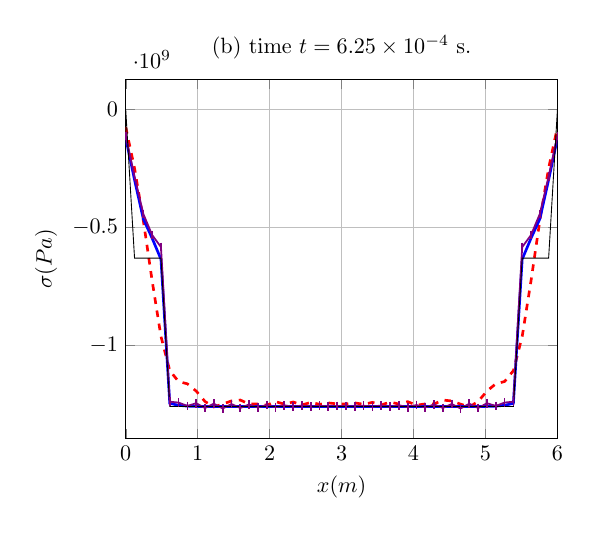
\begin{tikzpicture}[scale=0.8]
\begin{axis}[xlabel=$x (m)$,ylabel=$\sigma (Pa)$,ymajorgrids=true,xmajorgrids=true,legend pos=outer north east,title={(b) time $t = 6.25\times 10^{-4} $ s.},xmin=0.,xmax=6.]
\addplot[Red,very thick,mark=none,dashed] coordinates {(0.0,-74686690.65430246) (0.12244897959183673,-248860978.1693335) (0.24489795918367346,-471505677.3136862) (0.36734693877551017,-727347550.4714894) (0.4897959183673469,-963308331.6520433) (0.6122448979591837,-1108824904.6085515) (0.7346938775510203,-1154837713.915547) (0.8571428571428571,-1164658358.6882505) (0.9795918367346939,-1195327833.6731591) (1.1020408163265305,-1239722495.17177) (1.2244897959183674,-1262625036.5763078) (1.346938775510204,-1250850727.3360605) (1.4693877551020407,-1237335621.1098552) (1.5918367346938775,-1233570784.670482) (1.7142857142857142,-1250022356.590519) (1.836734693877551,-1250064510.2383804) (1.9591836734693877,-1255304260.9119728) (2.0816326530612246,-1240464014.9742188) (2.204081632653061,-1250749408.0219655) (2.326530612244898,-1241771881.0316234) (2.4489795918367347,-1254655253.5739675) (2.571428571428571,-1243386642.1602688) (2.693877551020408,-1251564997.8232079) (2.816326530612245,-1245650942.428049) (2.9387755102040813,-1249901934.3884947) (3.061224489795918,-1249901934.3884926) (3.183673469387755,-1245650942.4280505) (3.306122448979592,-1251564997.8232062) (3.4285714285714284,-1243386642.160271) (3.5510204081632653,-1254655253.5739667) (3.673469387755102,-1241771881.0316243) (3.7959183673469385,-1250749408.0219643) (3.9183673469387754,-1240464014.9742193) (4.040816326530612,-1255304260.911973) (4.163265306122449,-1250064510.238382) (4.285714285714286,-1250022356.59052) (4.408163265306122,-1233570784.670483) (4.530612244897959,-1237335621.1098552) (4.653061224489796,-1250850727.3360612) (4.775510204081632,-1262625036.5763083) (4.8979591836734695,-1239722495.1717708) (5.020408163265306,-1195327833.6731594) (5.142857142857142,-1164658358.688251) (5.26530612244898,-1154837713.915547) (5.387755102040816,-1108824904.6085508) (5.5102040816326525,-963308331.652042) (5.63265306122449,-727347550.4714878) (5.755102040816326,-471505677.3136848) (5.877551020408163,-248860978.16933236) (6.0,-74686690.65430167) };
\addplot[Blue,very thick,mark=none,solid] coordinates {(0.0,-120597397.19248778) (0.12244897959183673,-298539345.15508544) (0.24489795918367346,-464504460.170754) (0.36734693877551017,-546627376.3559334) (0.4897959183673469,-635546108.2543886) (0.6122448979591837,-1247334335.3333962) (0.7346938775510203,-1255980074.5990539) (0.8571428571428571,-1259371705.5275755) (0.9795918367346939,-1260535220.1287405) (1.1020408163265305,-1260885267.5005968) (1.2244897959183674,-1260977777.705495) (1.346938775510204,-1260999265.6570995) (1.4693877551020407,-1261003650.0375175) (1.5918367346938775,-1261004434.5740557) (1.7142857142857142,-1261004557.3391547) (1.836734693877551,-1261004574.0682204) (1.9591836734693877,-1261004576.0419452) (2.0816326530612246,-1261004576.241996) (2.204081632653061,-1261004576.2592359) (2.326530612244898,-1261004576.260481) (2.4489795918367347,-1261004576.260556) (2.571428571428571,-1261004576.2605588) (2.693877551020408,-1261004576.260559) (2.816326530612245,-1261004576.2605588) (2.9387755102040813,-1261004576.260559) (3.061224489795918,-1261004576.2605584) (3.183673469387755,-1261004576.2605586) (3.306122448979592,-1261004576.2605588) (3.4285714285714284,-1261004576.2605581) (3.5510204081632653,-1261004576.2605555) (3.673469387755102,-1261004576.260481) (3.7959183673469385,-1261004576.2592354) (3.9183673469387754,-1261004576.2419953) (4.040816326530612,-1261004576.0419443) (4.163265306122449,-1261004574.06822) (4.285714285714286,-1261004557.3391542) (4.408163265306122,-1261004434.5740552) (4.530612244897959,-1261003650.037517) (4.653061224489796,-1260999265.6570988) (4.775510204081632,-1260977777.7054946) (4.8979591836734695,-1260885267.500596) (5.020408163265306,-1260535220.1287398) (5.142857142857142,-1259371705.5275738) (5.26530612244898,-1255980074.5990536) (5.387755102040816,-1247334335.3333952) (5.5102040816326525,-635546108.2543867) (5.63265306122449,-546627376.3559326) (5.755102040816326,-464504460.1707534) (5.877551020408163,-298539345.15508515) (6.0,-120597397.19248791) };
\addplot[Purple,thick,mark=|,solid] coordinates {(0.0,-111808132.50928691) (0.12244897959183673,-283652980.311345) (0.24489795918367346,-443221012.94130766) (0.36734693877551017,-532712483.6212361) (0.4897959183673469,-583780738.0952947) (0.6122448979591837,-1240572116.142149) (0.7346938775510203,-1244261651.762744) (0.8571428571428571,-1258556998.8403206) (0.9795918367346939,-1246923690.2991939) (1.1020408163265305,-1267582002.156853) (1.2244897959183674,-1248919510.011234) (1.346938775510204,-1269351209.0749319) (1.4693877551020407,-1250347534.9609652) (1.5918367346938775,-1267308507.8062203) (1.7142857142857142,-1252234928.1894917) (1.836734693877551,-1265091742.2400982) (1.9591836734693877,-1254542095.0106862) (2.0816326530612246,-1263677501.5970206) (2.204081632653061,-1255669724.044529) (2.326530612244898,-1262623936.670721) (2.4489795918367347,-1256618647.3458264) (2.571428571428571,-1261747368.978006) (2.693877551020408,-1257589986.0890632) (2.816326530612245,-1260580011.675211) (2.9387755102040813,-1258915831.3187945) (3.061224489795918,-1258915831.3187914) (3.183673469387755,-1260580011.6752121) (3.306122448979592,-1257589986.0890625) (3.4285714285714284,-1261747368.9780068) (3.5510204081632653,-1256618647.3458252) (3.673469387755102,-1262623936.6707222) (3.7959183673469385,-1255669724.0445278) (3.9183673469387754,-1263677501.5970201) (4.040816326530612,-1254542095.0106847) (4.163265306122449,-1265091742.2400992) (4.285714285714286,-1252234928.1894906) (4.408163265306122,-1267308507.80622) (4.530612244897959,-1250347534.9609656) (4.653061224489796,-1269351209.0749316) (4.775510204081632,-1248919510.0112329) (4.8979591836734695,-1267582002.1568534) (5.020408163265306,-1246923690.2991939) (5.142857142857142,-1258556998.8403208) (5.26530612244898,-1244261651.7627428) (5.387755102040816,-1240572116.1421485) (5.5102040816326525,-583780738.0952928) (5.63265306122449,-532712483.6212349) (5.755102040816326,-443221012.9413062) (5.877551020408163,-283652980.3113445) (6.0,-111808132.50928625) };
\addplot[black,thin,mark=none,solid] coordinates {(0.0,-0.0) (0.12244897959183673,-630502288.1302795) (0.24489795918367346,-630502288.1302795) (0.36734693877551017,-630502288.1302795) (0.4897959183673469,-630502288.1302795) (0.6122448979591837,-1261004576.260559) (0.7346938775510203,-1261004576.260559) (0.8571428571428571,-1261004576.260559) (0.9795918367346939,-1261004576.260559) (1.1020408163265305,-1261004576.260559) (1.2244897959183674,-1261004576.260559) (1.346938775510204,-1261004576.260559) (1.4693877551020407,-1261004576.260559) (1.5918367346938775,-1261004576.260559) (1.7142857142857142,-1261004576.260559) (1.836734693877551,-1261004576.260559) (1.9591836734693877,-1261004576.260559) (2.0816326530612246,-1261004576.260559) (2.204081632653061,-1261004576.260559) (2.326530612244898,-1261004576.260559) (2.4489795918367347,-1261004576.260559) (2.571428571428571,-1261004576.260559) (2.693877551020408,-1261004576.260559) (2.816326530612245,-1261004576.260559) (2.9387755102040813,-1261004576.260559) (3.061224489795918,-1261004576.260559) (3.183673469387755,-1261004576.260559) (3.306122448979592,-1261004576.260559) (3.4285714285714284,-1261004576.260559) (3.5510204081632653,-1261004576.260559) (3.673469387755102,-1261004576.260559) (3.7959183673469385,-1261004576.260559) (3.9183673469387754,-1261004576.260559) (4.040816326530612,-1261004576.260559) (4.163265306122449,-1261004576.260559) (4.285714285714286,-1261004576.260559) (4.408163265306122,-1261004576.260559) (4.530612244897959,-1261004576.260559) (4.653061224489796,-1261004576.260559) (4.775510204081632,-1261004576.260559) (4.8979591836734695,-1261004576.260559) (5.020408163265306,-1261004576.260559) (5.142857142857142,-1261004576.260559) (5.26530612244898,-1261004576.260559) (5.387755102040816,-1261004576.260559) (5.5102040816326525,-630502288.1302795) (5.63265306122449,-630502288.1302795) (5.755102040816326,-630502288.1302795) (5.877551020408163,-630502288.1302795) (6.0,-0.0) };
%\legend{usl 1ppc,dgmpm 1ppc (ep solver),dgmpm 1ppc (ac solver),exact}
\end{axis}
\end{tikzpicture}
%%% Local Variables:
%%% mode: latex
%%% TeX-master: "../../mainManuscript"
%%% End:
}
  {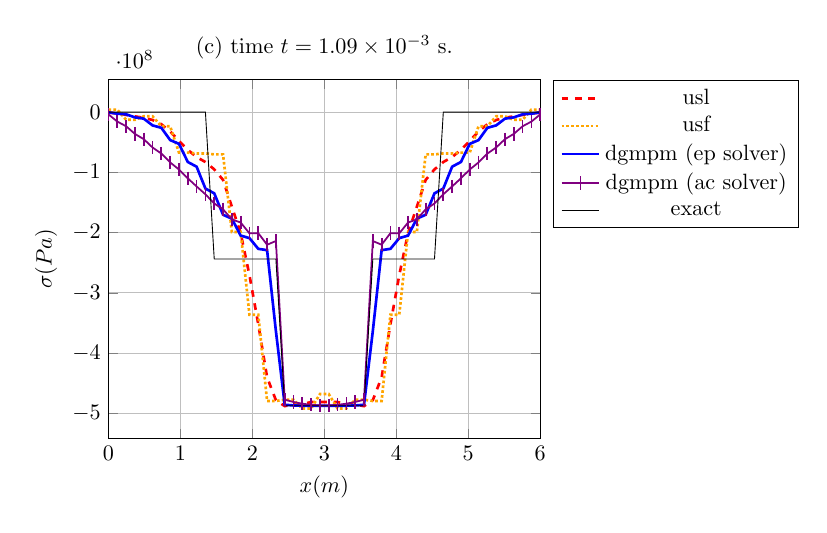
\begin{tikzpicture}[scale=0.8]
\begin{axis}[xlabel=$x (m)$,ylabel=$\sigma (Pa)$,ymajorgrids=true,xmajorgrids=true,legend pos=outer north east,title={(c) time $t = 1.09\times 10^{-3} $ s.},xmin=0.,xmax=6.]
\addplot[Red,very thick,mark=none,dashed,mark size=3pt] coordinates {(0.0,-679166.0601331755) (0.12244897959183673,-2368189.594188208) (0.24489795918367346,-4606456.556212341) (0.36734693877551017,-6961578.395676694) (0.4897959183673469,-9332760.287028607) (0.6122448979591837,-12938682.464591796) (0.7346938775510203,-20102821.471402142) (0.8571428571428571,-32015823.341737133) (0.9795918367346939,-47676454.15860757) (1.1020408163265305,-62502940.42234602) (1.2244897959183674,-74544680.06037714) (1.346938775510204,-82775603.38522142) (1.4693877551020407,-94947363.4179823) (1.5918367346938775,-112415785.44002911) (1.7142857142857142,-156774491.63523546) (1.836734693877551,-200654618.50473383) (1.9591836734693877,-270646588.3413816) (2.0816326530612246,-351928629.9311485) (2.204081632653061,-440064160.15512294) (2.326530612244898,-477934424.91056436) (2.4489795918367347,-487815276.0764712) (2.571428571428571,-485351241.33413374) (2.693877551020408,-484406188.97201383) (2.816326530612245,-481035531.7602433) (2.9387755102040813,-481038509.8228564) (3.061224489795918,-481038509.8228558) (3.183673469387755,-481035531.7602443) (3.306122448979592,-484406188.9720135) (3.4285714285714284,-485351241.3341341) (3.5510204081632653,-487815276.07647014) (3.673469387755102,-477934424.9105651) (3.7959183673469385,-440064160.15512156) (3.9183673469387754,-351928629.931148) (4.040816326530612,-270646588.34138024) (4.163265306122449,-200654618.50473374) (4.285714285714286,-156774491.63523474) (4.408163265306122,-112415785.44002907) (4.530612244897959,-94947363.41798277) (4.653061224489796,-82775603.38522187) (4.775510204081632,-74544680.06037733) (4.8979591836734695,-62502940.42234604) (5.020408163265306,-47676454.158607304) (5.142857142857142,-32015823.341736842) (5.26530612244898,-20102821.471402) (5.387755102040816,-12938682.46459166) (5.5102040816326525,-9332760.287028512) (5.63265306122449,-6961578.395676572) (5.755102040816326,-4606456.55621225) (5.877551020408163,-2368189.594188123) (6.0,-679166.0601331636) };
\addplot[Orange,very thick,mark=none,densely dotted,mark size=3pt] coordinates {(0.0,4236951.290463989) (0.12244897959183673,4236951.290460123) (0.24489795918367346,-12679253.938911917) (0.36734693877551017,-12679253.938916743) (0.4897959183673469,-6922591.558428046) (0.6122448979591837,-6922591.558431343) (0.7346938775510203,-23459809.182112668) (0.8571428571428571,-23459809.18211712) (0.9795918367346939,-67167151.83770859) (1.1020408163265305,-67167151.83771148) (1.2244897959183674,-68479697.03436251) (1.346938775510204,-68479697.03436783) (1.4693877551020407,-70089580.65292576) (1.5918367346938775,-70089580.65292576) (1.7142857142857142,-198942113.00187883) (1.836734693877551,-198942113.00187835) (1.9591836734693877,-336192669.59109914) (2.0816326530612246,-336192669.59109795) (2.204081632653061,-479279910.7951127) (2.326530612244898,-479279910.795111) (2.4489795918367347,-477181511.2029586) (2.571428571428571,-477181511.20295614) (2.693877551020408,-491728219.61058974) (2.816326530612245,-491728219.6105894) (2.9387755102040813,-467835686.5023686) (3.061224489795918,-467835686.50236756) (3.183673469387755,-491728219.6105915) (3.306122448979592,-491728219.61058766) (3.4285714285714284,-477181511.20295787) (3.5510204081632653,-477181511.20295686) (3.673469387755102,-479279910.79511243) (3.7959183673469385,-479279910.7951107) (3.9183673469387754,-336192669.5910962) (4.040816326530612,-336192669.59110004) (4.163265306122449,-198942113.0018753) (4.285714285714286,-198942113.00188202) (4.408163265306122,-70089580.65291941) (4.530612244897959,-70089580.65293229) (4.653061224489796,-68479697.03436142) (4.775510204081632,-68479697.03436944) (4.8979591836734695,-67167151.83770534) (5.020408163265306,-67167151.83771467) (5.142857142857142,-23459809.182109676) (5.26530612244898,-23459809.182119854) (5.387755102040816,-6922591.558424118) (5.5102040816326525,-6922591.558435734) (5.63265306122449,-12679253.938909372) (5.755102040816326,-12679253.938918298) (5.877551020408163,4236951.290467103) (6.0,4236951.290456754) };
\addplot[Blue,very thick,mark=none,solid,mark size=3pt] coordinates {(0.0,-298852.1952411225) (0.12244897959183673,-2592980.4740912793) (0.24489795918367346,-3560236.4322381816) (0.36734693877551017,-8652722.221047912) (0.4897959183673469,-10777216.673686886) (0.6122448979591837,-21974314.707157355) (0.7346938775510203,-26009924.918005344) (0.8571428571428571,-46347563.10657899) (0.9795918367346939,-52593345.171819046) (1.1020408163265305,-82683979.65035231) (1.2244897959183674,-90525380.97285904) (1.346938775510204,-126773557.44849168) (1.4693877551020407,-134743667.28836828) (1.5918367346938775,-170219249.4978279) (1.7142857142857142,-176744937.7749974) (1.836734693877551,-204799464.24688196) (1.9591836734693877,-209064122.25232974) (2.0816326530612246,-226820170.49378502) (2.204081632653061,-229011964.3130221) (2.326530612244898,-363270795.9137317) (2.4489795918367347,-485529213.90073514) (2.571428571428571,-486748760.1951447) (2.693877551020408,-487164866.56783277) (2.816326530612245,-487268871.16624963) (2.9387755102040813,-487285807.7274521) (3.061224489795918,-487285807.7274521) (3.183673469387755,-487268871.16624963) (3.306122448979592,-487164866.56783277) (3.4285714285714284,-486748760.1951447) (3.5510204081632653,-485529213.90073514) (3.673469387755102,-363270795.91372997) (3.7959183673469385,-229011964.3130223) (3.9183673469387754,-226820170.49378502) (4.040816326530612,-209064122.25232938) (4.163265306122449,-204799464.2468816) (4.285714285714286,-176744937.77499697) (4.408163265306122,-170219249.4978276) (4.530612244897959,-134743667.28836808) (4.653061224489796,-126773557.44849148) (4.775510204081632,-90525380.9728589) (4.8979591836734695,-82683979.65035222) (5.020408163265306,-52593345.171819076) (5.142857142857142,-46347563.10657902) (5.26530612244898,-26009924.918005634) (5.387755102040816,-21974314.707157686) (5.5102040816326525,-10777216.673687106) (5.63265306122449,-8652722.22104813) (5.755102040816326,-3560236.4322383474) (5.877551020408163,-2592980.4740913147) (6.0,-298852.1952412414) };
\addplot[Purple,thick,mark=|,solid,mark size=3pt] coordinates {(0.0,-3699822.6801933693) (0.12244897959183673,-15656690.657919873) (0.24489795918367346,-23395010.37401582) (0.36734693877551017,-36103443.51008522) (0.4897959183673469,-44799564.7059784) (0.6122448979591837,-58626001.393915564) (0.7346938775510203,-68743311.52420163) (0.8571428571428571,-83413570.25799192) (0.9795918367346939,-95210786.60876837) (1.1020408163265305,-109767206.98229863) (1.2244897959183674,-123307254.49744721) (1.346938775510204,-136286963.85824355) (1.4693877551020407,-151490220.183104) (1.5918367346938775,-161259604.24498996) (1.7142857142857142,-177973600.29101613) (1.836734693877551,-183108322.81917205) (1.9591836734693877,-201165134.12201387) (2.0816326530612246,-200760737.51095787) (2.204081632653061,-220004370.6130868) (2.326530612244898,-213836576.44044873) (2.4489795918367347,-477124042.8840971) (2.571428571428571,-480953140.1350389) (2.693877551020408,-483830928.1925999) (2.816326530612245,-485620834.2660387) (2.9387755102040813,-486699217.4934911) (3.061224489795918,-486699217.4934911) (3.183673469387755,-485620834.2660387) (3.306122448979592,-483830928.1925999) (3.4285714285714284,-480953140.1350389) (3.5510204081632653,-477124042.8840971) (3.673469387755102,-213836576.44044736) (3.7959183673469385,-220004370.6130868) (3.9183673469387754,-200760737.5109577) (4.040816326530612,-201165134.1220135) (4.163265306122449,-183108322.81917205) (4.285714285714286,-177973600.2910157) (4.408163265306122,-161259604.24498972) (4.530612244897959,-151490220.18310383) (4.653061224489796,-136286963.85824338) (4.775510204081632,-123307254.49744716) (4.8979591836734695,-109767206.98229855) (5.020408163265306,-95210786.6087684) (5.142857142857142,-83413570.25799206) (5.26530612244898,-68743311.52420157) (5.387755102040816,-58626001.393915735) (5.5102040816326525,-44799564.70597822) (5.63265306122449,-36103443.51008532) (5.755102040816326,-23395010.374015827) (5.877551020408163,-15656690.657920003) (6.0,-3699822.6801932575) };
\addplot[black,thin,mark=none,solid,mark size=3pt] coordinates {(0.0,-0.0) (0.12244897959183673,-0.0) (0.24489795918367346,-0.0) (0.36734693877551017,-0.0) (0.4897959183673469,-0.0) (0.6122448979591837,-0.0) (0.7346938775510203,-0.0) (0.8571428571428571,-0.0) (0.9795918367346939,-0.0) (1.1020408163265305,-0.0) (1.2244897959183674,-0.0) (1.346938775510204,-0.0) (1.4693877551020407,-243643578.04719847) (1.5918367346938775,-243643578.04719847) (1.7142857142857142,-243643578.04719847) (1.836734693877551,-243643578.04719847) (1.9591836734693877,-243643578.04719847) (2.0816326530612246,-243643578.04719847) (2.204081632653061,-243643578.04719847) (2.326530612244898,-243643578.04719847) (2.4489795918367347,-487287156.09439695) (2.571428571428571,-487287156.09439695) (2.693877551020408,-487287156.09439695) (2.816326530612245,-487287156.09439695) (2.9387755102040813,-487287156.09439695) (3.061224489795918,-487287156.09439695) (3.183673469387755,-487287156.09439695) (3.306122448979592,-487287156.09439695) (3.4285714285714284,-487287156.09439695) (3.5510204081632653,-487287156.09439695) (3.673469387755102,-243643578.04719847) (3.7959183673469385,-243643578.04719847) (3.9183673469387754,-243643578.04719847) (4.040816326530612,-243643578.04719847) (4.163265306122449,-243643578.04719847) (4.285714285714286,-243643578.04719847) (4.408163265306122,-243643578.04719847) (4.530612244897959,-243643578.04719847) (4.653061224489796,-0.0) (4.775510204081632,-0.0) (4.8979591836734695,-0.0) (5.020408163265306,-0.0) (5.142857142857142,-0.0) (5.26530612244898,-0.0) (5.387755102040816,-0.0) (5.5102040816326525,-0.0) (5.63265306122449,-0.0) (5.755102040816326,-0.0) (5.877551020408163,-0.0) (6.0,-0.0) };
\legend{usl,usf,dgmpm (ep solver),dgmpm (ac solver),exact}
\end{axis}
\end{tikzpicture}
%%% Local Variables:
%%% mode: latex
%%% TeX-master: "../../mainManuscript"
%%% End:
}
  \caption{elastic-plastic RP stress}
  \label{fig:stress_elastoplastic_RP}
\end{figure}
\begin{figure}[h!]
  \centering
  {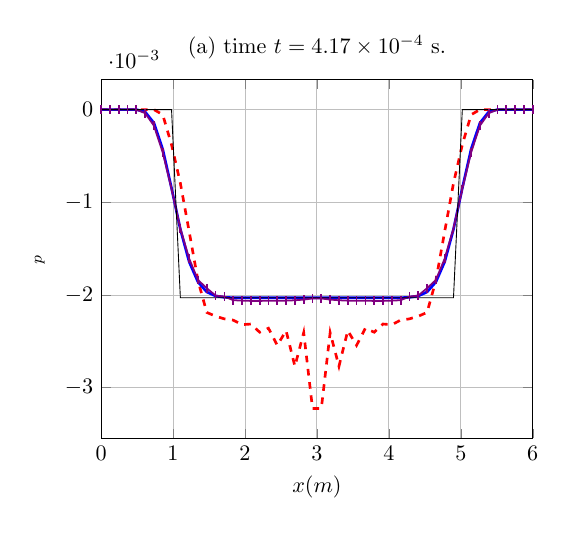
\begin{tikzpicture}[scale=0.8]
\begin{axis}[xlabel=$x (m)$,ylabel=$\eps^p$,ymajorgrids=true,xmajorgrids=true,legend pos=outer north east,title={(a) time $t = 4.17\times 10^{-4} $ s.},xmin=0.,xmax=6.]
\addplot[Red,very thick,mark=none,dashed] coordinates {(0.0,0.0) (0.12244897959183673,0.0) (0.24489795918367346,0.0) (0.36734693877551017,0.0) (0.4897959183673469,0.0) (0.6122448979591837,0.0) (0.7346938775510203,0.0) (0.8571428571428571,-5.5177825258810104e-05) (0.9795918367346939,-0.0003791196239632164) (1.1020408163265305,-0.0007942218458547296) (1.2244897959183674,-0.0013158519965027296) (1.346938775510204,-0.0018458090676901286) (1.4693877551020407,-0.002188794617508559) (1.5918367346938775,-0.002229697455331896) (1.7142857142857142,-0.002258121963594508) (1.836734693877551,-0.002271799079674154) (1.9591836734693877,-0.002320613632318322) (2.0816326530612246,-0.002313868472160546) (2.204081632653061,-0.0024020122032007017) (2.326530612244898,-0.0023588630990294623) (2.4489795918367347,-0.0025433455597807667) (2.571428571428571,-0.002385435935351422) (2.693877551020408,-0.0027693350417516906) (2.816326530612245,-0.0024065265204776445) (2.9387755102040813,-0.0032250612006492966) (3.061224489795918,-0.0032250612006492524) (3.183673469387755,-0.002406526520477666) (3.306122448979592,-0.0027693350417516823) (3.4285714285714284,-0.0023854359353514295) (3.5510204081632653,-0.0025433455597807628) (3.673469387755102,-0.002358863099029464) (3.7959183673469385,-0.0024020122032006983) (3.9183673469387754,-0.0023138684721605448) (4.040816326530612,-0.002320613632318319) (4.163265306122449,-0.0022717990796741546) (4.285714285714286,-0.0022581219635945077) (4.408163265306122,-0.0022296974553318956) (4.530612244897959,-0.0021887946175085595) (4.653061224489796,-0.001845809067690125) (4.775510204081632,-0.0013158519965027254) (4.8979591836734695,-0.0007942218458547295) (5.020408163265306,-0.0003791196239632123) (5.142857142857142,-5.5177825258808404e-05) (5.26530612244898,0.0) (5.387755102040816,0.0) (5.5102040816326525,0.0) (5.63265306122449,0.0) (5.755102040816326,0.0) (5.877551020408163,0.0) (6.0,0.0) };
\addplot[Blue,very thick,mark=none,solid] coordinates {(0.0,0.0) (0.12244897959183673,0.0) (0.24489795918367346,0.0) (0.36734693877551017,0.0) (0.4897959183673469,0.0) (0.6122448979591837,-2.4267855226065594e-05) (0.7346938775510203,-0.00014452073597361284) (0.8571428571428571,-0.0004275642401009131) (0.9795918367346939,-0.0008483282066457896) (1.1020408163265305,-0.0012913872123487611) (1.2244897959183674,-0.001642660920094959) (1.346938775510204,-0.0018602413103573651) (1.4693877551020407,-0.0019680574666657586) (1.5918367346938775,-0.00201146561977191) (1.7142857142857142,-0.002025805454394895) (1.836734693877551,-0.0020297136017104972) (1.9591836734693877,-0.002030593864489664) (2.0816326530612246,-0.002030757436013639) (2.204081632653061,-0.0020307823755532774) (2.326530612244898,-0.002030785465084119) (2.4489795918367347,-0.0020307857712710334) (2.571428571428571,-0.00203078579497771) (2.693877551020408,-0.0020307857963597366) (2.816326530612245,-0.002030785796416807) (2.9387755102040813,-0.002030785796418294) (3.061224489795918,-0.002030785796418294) (3.183673469387755,-0.0020307857964168056) (3.306122448979592,-0.002030785796359739) (3.4285714285714284,-0.0020307857949777124) (3.5510204081632653,-0.002030785771271032) (3.673469387755102,-0.002030785465084119) (3.7959183673469385,-0.002030782375553277) (3.9183673469387754,-0.0020307574360136386) (4.040816326530612,-0.002030593864489664) (4.163265306122449,-0.0020297136017104964) (4.285714285714286,-0.0020258054543948927) (4.408163265306122,-0.002011465619771909) (4.530612244897959,-0.0019680574666657573) (4.653061224489796,-0.0018602413103573651) (4.775510204081632,-0.0016426609200949592) (4.8979591836734695,-0.001291387212348762) (5.020408163265306,-0.0008483282066457893) (5.142857142857142,-0.00042756424010091193) (5.26530612244898,-0.00014452073597361384) (5.387755102040816,-2.4267855226067292e-05) (5.5102040816326525,0.0) (5.63265306122449,0.0) (5.755102040816326,0.0) (5.877551020408163,0.0) (6.0,0.0) };
\addplot[Purple,thick,mark=|,solid] coordinates {(0.0,0.0) (0.12244897959183673,0.0) (0.24489795918367346,0.0) (0.36734693877551017,0.0) (0.4897959183673469,0.0) (0.6122448979591837,-3.850800809337606e-05) (0.7346938775510203,-0.00017337094943683953) (0.8571428571428571,-0.00046273089543238553) (0.9795918367346939,-0.000857123655577256) (1.1020408163265305,-0.0012817129348415013) (1.2244897959183674,-0.0016077047572306) (1.346938775510204,-0.0018386451535459692) (1.4693877551020407,-0.0019271405531036338) (1.5918367346938775,-0.002006348337646142) (1.7142857142857142,-0.002018045326373221) (1.836734693877551,-0.002056615251608797) (1.9591836734693877,-0.0020613216365693464) (2.0816326530612246,-0.002064203896841495) (2.204081632653061,-0.0020644266901542695) (2.326530612244898,-0.0020621094945296272) (2.4489795918367347,-0.002062767607181189) (2.571428571428571,-0.002061489252343496) (2.693877551020408,-0.0020573197208032658) (2.816326530612245,-0.0020502799029179) (2.9387755102040813,-0.0020377776694292327) (3.061224489795918,-0.0020377776694292327) (3.183673469387755,-0.002050279902917899) (3.306122448979592,-0.002057319720803265) (3.4285714285714284,-0.0020614892523434956) (3.5510204081632653,-0.0020627676071811878) (3.673469387755102,-0.0020621094945296285) (3.7959183673469385,-0.0020644266901542695) (3.9183673469387754,-0.0020642038968414953) (4.040816326530612,-0.0020613216365693477) (4.163265306122449,-0.002056615251608799) (4.285714285714286,-0.0020180453263732205) (4.408163265306122,-0.0020063483376461405) (4.530612244897959,-0.0019271405531036334) (4.653061224489796,-0.0018386451535459673) (4.775510204081632,-0.0016077047572305996) (4.8979591836734695,-0.0012817129348415002) (5.020408163265306,-0.0008571236555772557) (5.142857142857142,-0.000462730895432386) (5.26530612244898,-0.0001733709494368422) (5.387755102040816,-3.850800809337776e-05) (5.5102040816326525,0.0) (5.63265306122449,0.0) (5.755102040816326,0.0) (5.877551020408163,0.0) (6.0,0.0) };
\addplot[black,thin,mark=none,solid] coordinates {(0.0,-0.0) (0.12244897959183673,-0.0) (0.24489795918367346,-0.0) (0.36734693877551017,-0.0) (0.4897959183673469,-0.0) (0.6122448979591837,-0.0) (0.7346938775510203,-0.0) (0.8571428571428571,-0.0) (0.9795918367346939,-0.0) (1.1020408163265305,-0.002030785796418313) (1.2244897959183674,-0.002030785796418313) (1.346938775510204,-0.002030785796418313) (1.4693877551020407,-0.002030785796418313) (1.5918367346938775,-0.002030785796418313) (1.7142857142857142,-0.002030785796418313) (1.836734693877551,-0.002030785796418313) (1.9591836734693877,-0.002030785796418313) (2.0816326530612246,-0.002030785796418313) (2.204081632653061,-0.002030785796418313) (2.326530612244898,-0.002030785796418313) (2.4489795918367347,-0.002030785796418313) (2.571428571428571,-0.002030785796418313) (2.693877551020408,-0.002030785796418313) (2.816326530612245,-0.002030785796418313) (2.9387755102040813,-0.002030785796418313) (3.061224489795918,-0.002030785796418313) (3.183673469387755,-0.002030785796418313) (3.306122448979592,-0.002030785796418313) (3.4285714285714284,-0.002030785796418313) (3.5510204081632653,-0.002030785796418313) (3.673469387755102,-0.002030785796418313) (3.7959183673469385,-0.002030785796418313) (3.9183673469387754,-0.002030785796418313) (4.040816326530612,-0.002030785796418313) (4.163265306122449,-0.002030785796418313) (4.285714285714286,-0.002030785796418313) (4.408163265306122,-0.002030785796418313) (4.530612244897959,-0.002030785796418313) (4.653061224489796,-0.002030785796418313) (4.775510204081632,-0.002030785796418313) (4.8979591836734695,-0.002030785796418313) (5.020408163265306,-0.0) (5.142857142857142,-0.0) (5.26530612244898,-0.0) (5.387755102040816,-0.0) (5.5102040816326525,-0.0) (5.63265306122449,-0.0) (5.755102040816326,-0.0) (5.877551020408163,-0.0) (6.0,-0.0) };
%\legend{usl 1ppc,dgmpm 1ppc (ep solver),dgmpm 1ppc (ac solver),exact}
\end{axis}
\end{tikzpicture}
%%% Local Variables:
%%% mode: latex
%%% TeX-master: "../../mainManuscript"
%%% End:
}
  {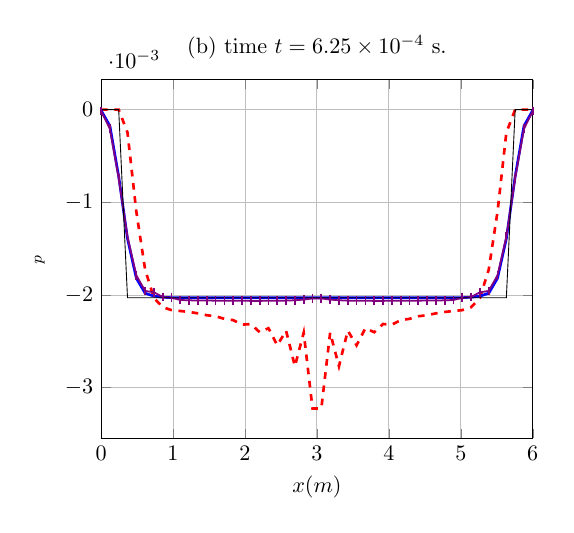
\begin{tikzpicture}[scale=0.8]
\begin{axis}[xlabel=$x (m)$,ylabel=$\eps^p$,ymajorgrids=true,xmajorgrids=true,legend pos=outer north east,title={(b) time $t = 6.25\times 10^{-4} $ s.},xmin=0.,xmax=6.]
\addplot[Red,very thick,mark=none,dashed] coordinates {(0.0,0.0) (0.12244897959183673,0.0) (0.24489795918367346,0.0) (0.36734693877551017,-0.0002478348228815541) (0.4897959183673469,-0.0011004378155012712) (0.6122448979591837,-0.0017260409269248597) (0.7346938775510203,-0.002031865332982762) (0.8571428571428571,-0.002132968518977378) (0.9795918367346939,-0.0021636018350532395) (1.1020408163265305,-0.0021733079916121177) (1.2244897959183674,-0.00218350748748031) (1.346938775510204,-0.002198645448466017) (1.4693877551020407,-0.002218920213241705) (1.5918367346938775,-0.002229697455331896) (1.7142857142857142,-0.002258121963594508) (1.836734693877551,-0.002271799079674154) (1.9591836734693877,-0.002320613632318322) (2.0816326530612246,-0.002313868472160546) (2.204081632653061,-0.0024020122032007017) (2.326530612244898,-0.0023588630990294623) (2.4489795918367347,-0.0025433455597807667) (2.571428571428571,-0.002385435935351422) (2.693877551020408,-0.0027693350417516906) (2.816326530612245,-0.0024065265204776445) (2.9387755102040813,-0.0032250612006492966) (3.061224489795918,-0.0032250612006492524) (3.183673469387755,-0.002406526520477666) (3.306122448979592,-0.0027693350417516823) (3.4285714285714284,-0.0023854359353514295) (3.5510204081632653,-0.0025433455597807628) (3.673469387755102,-0.002358863099029464) (3.7959183673469385,-0.0024020122032006983) (3.9183673469387754,-0.0023138684721605448) (4.040816326530612,-0.002320613632318319) (4.163265306122449,-0.0022717990796741546) (4.285714285714286,-0.0022581219635945077) (4.408163265306122,-0.0022296974553318956) (4.530612244897959,-0.0022189202132417056) (4.653061224489796,-0.0021986454484660173) (4.775510204081632,-0.0021835074874803095) (4.8979591836734695,-0.0021733079916121186) (5.020408163265306,-0.0021636018350532395) (5.142857142857142,-0.002132968518977378) (5.26530612244898,-0.002031865332982763) (5.387755102040816,-0.0017260409269248577) (5.5102040816326525,-0.0011004378155012658) (5.63265306122449,-0.0002478348228815494) (5.755102040816326,0.0) (5.877551020408163,0.0) (6.0,0.0) };
\addplot[Blue,very thick,mark=none,solid] coordinates {(0.0,-8.02367288935203e-06) (0.12244897959183673,-0.00017614426387335805) (0.24489795918367346,-0.0007207542691858686) (0.36734693877551017,-0.0013919930410856215) (0.4897959183673469,-0.001818355598439618) (0.6122448979591837,-0.001981300761387861) (0.7346938775510203,-0.0020125975551096974) (0.8571428571428571,-0.002024874952136019) (0.9795918367346939,-0.0020290867696967987) (1.1020408163265305,-0.002030353909504423) (1.2244897959183674,-0.0020306887880741907) (1.346938775510204,-0.0020307665725143873) (1.4693877551020407,-0.0020307824435747243) (1.5918367346938775,-0.0020307852835259937) (1.7142857142857142,-0.0020307857279245408) (1.836734693877551,-0.0020307857884822454) (1.9591836734693877,-0.00203078579562695) (2.0816326530612246,-0.002030785796351117) (2.204081632653061,-0.0020307857964135248) (2.326530612244898,-0.002030785796418031) (2.4489795918367347,-0.002030785796418302) (2.571428571428571,-0.0020307857964183135) (2.693877551020408,-0.002030785796418313) (2.816326530612245,-0.002030785796418313) (2.9387755102040813,-0.002030785796418314) (3.061224489795918,-0.0020307857964183135) (3.183673469387755,-0.0020307857964183135) (3.306122448979592,-0.0020307857964183126) (3.4285714285714284,-0.0020307857964183113) (3.5510204081632653,-0.0020307857964183005) (3.673469387755102,-0.002030785796418031) (3.7959183673469385,-0.0020307857964135217) (3.9183673469387754,-0.0020307857963511138) (4.040816326530612,-0.002030785795626948) (4.163265306122449,-0.0020307857884822433) (4.285714285714286,-0.0020307857279245403) (4.408163265306122,-0.0020307852835259915) (4.530612244897959,-0.0020307824435747226) (4.653061224489796,-0.0020307665725143842) (4.775510204081632,-0.002030688788074188) (4.8979591836734695,-0.0020303539095044196) (5.020408163265306,-0.0020290867696967953) (5.142857142857142,-0.0020248749521360144) (5.26530612244898,-0.0020125975551096966) (5.387755102040816,-0.0019813007613878565) (5.5102040816326525,-0.0018183555984396154) (5.63265306122449,-0.0013919930410856195) (5.755102040816326,-0.0007207542691858678) (5.877551020408163,-0.0001761442638733595) (6.0,-8.023672889353243e-06) };
\addplot[Purple,thick,mark=|,solid] coordinates {(0.0,-1.4376766038990375e-05) (0.12244897959183673,-0.0002078915703532438) (0.24489795918367346,-0.000740641579521879) (0.36734693877551017,-0.0013729886129224668) (0.4897959183673469,-0.001786873759629078) (0.6122448979591837,-0.0019568221398810824) (0.7346938775510203,-0.0019710253863315036) (0.8571428571428571,-0.002021925787657269) (0.9795918367346939,-0.00203043998544926) (1.1020408163265305,-0.002054595482920735) (1.2244897959183674,-0.0020576351166755064) (1.346938775510204,-0.0020609998518549564) (1.4693877551020407,-0.0020606031772355433) (1.5918367346938775,-0.002061501114574304) (1.7142857142857142,-0.002061887903336271) (1.836734693877551,-0.002062455598454706) (1.9591836734693877,-0.0020617923316583004) (2.0816326530612246,-0.002064203896841495) (2.204081632653061,-0.0020644266901542695) (2.326530612244898,-0.0020621094945296272) (2.4489795918367347,-0.002062767607181189) (2.571428571428571,-0.002061489252343496) (2.693877551020408,-0.0020573197208032658) (2.816326530612245,-0.0020502799029179) (2.9387755102040813,-0.0020377776694292327) (3.061224489795918,-0.0020377776694292327) (3.183673469387755,-0.002050279902917899) (3.306122448979592,-0.002057319720803265) (3.4285714285714284,-0.0020614892523434956) (3.5510204081632653,-0.0020627676071811878) (3.673469387755102,-0.0020621094945296285) (3.7959183673469385,-0.0020644266901542695) (3.9183673469387754,-0.0020642038968414953) (4.040816326530612,-0.0020617923316583004) (4.163265306122449,-0.002062455598454705) (4.285714285714286,-0.0020618879033362705) (4.408163265306122,-0.002061501114574307) (4.530612244897959,-0.0020606031772355464) (4.653061224489796,-0.002060999851854956) (4.775510204081632,-0.002057635116675507) (4.8979591836734695,-0.002054595482920736) (5.020408163265306,-0.002030439985449261) (5.142857142857142,-0.0020219257876572696) (5.26530612244898,-0.001971025386331503) (5.387755102040816,-0.0019568221398810802) (5.5102040816326525,-0.0017868737596290767) (5.63265306122449,-0.0013729886129224679) (5.755102040816326,-0.0007406415795218811) (5.877551020408163,-0.00020789157035324622) (6.0,-1.4376766038991588e-05) };
\addplot[black,thin,mark=none,solid] coordinates {(0.0,-0.0) (0.12244897959183673,-0.0) (0.24489795918367346,-0.0) (0.36734693877551017,-0.002030785796418313) (0.4897959183673469,-0.002030785796418313) (0.6122448979591837,-0.002030785796418313) (0.7346938775510203,-0.002030785796418313) (0.8571428571428571,-0.002030785796418313) (0.9795918367346939,-0.002030785796418313) (1.1020408163265305,-0.002030785796418313) (1.2244897959183674,-0.002030785796418313) (1.346938775510204,-0.002030785796418313) (1.4693877551020407,-0.002030785796418313) (1.5918367346938775,-0.002030785796418313) (1.7142857142857142,-0.002030785796418313) (1.836734693877551,-0.002030785796418313) (1.9591836734693877,-0.002030785796418313) (2.0816326530612246,-0.002030785796418313) (2.204081632653061,-0.002030785796418313) (2.326530612244898,-0.002030785796418313) (2.4489795918367347,-0.002030785796418313) (2.571428571428571,-0.002030785796418313) (2.693877551020408,-0.002030785796418313) (2.816326530612245,-0.002030785796418313) (2.9387755102040813,-0.002030785796418313) (3.061224489795918,-0.002030785796418313) (3.183673469387755,-0.002030785796418313) (3.306122448979592,-0.002030785796418313) (3.4285714285714284,-0.002030785796418313) (3.5510204081632653,-0.002030785796418313) (3.673469387755102,-0.002030785796418313) (3.7959183673469385,-0.002030785796418313) (3.9183673469387754,-0.002030785796418313) (4.040816326530612,-0.002030785796418313) (4.163265306122449,-0.002030785796418313) (4.285714285714286,-0.002030785796418313) (4.408163265306122,-0.002030785796418313) (4.530612244897959,-0.002030785796418313) (4.653061224489796,-0.002030785796418313) (4.775510204081632,-0.002030785796418313) (4.8979591836734695,-0.002030785796418313) (5.020408163265306,-0.002030785796418313) (5.142857142857142,-0.002030785796418313) (5.26530612244898,-0.002030785796418313) (5.387755102040816,-0.002030785796418313) (5.5102040816326525,-0.002030785796418313) (5.63265306122449,-0.002030785796418313) (5.755102040816326,-0.0) (5.877551020408163,-0.0) (6.0,-0.0) };
%\legend{usl 1ppc,dgmpm 1ppc (ep solver),dgmpm 1ppc (ac solver),exact}
\end{axis}
\end{tikzpicture}
%%% Local Variables:
%%% mode: latex
%%% TeX-master: "../../mainManuscript"
%%% End:
}
  {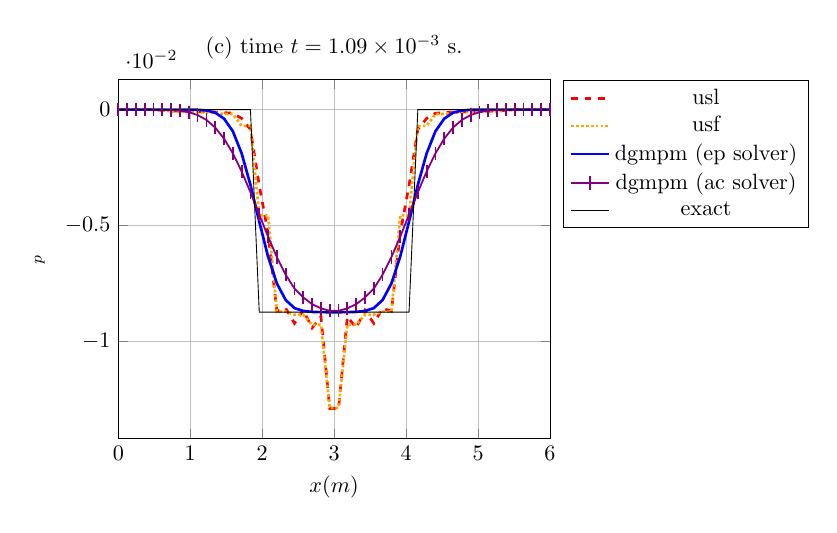
\begin{tikzpicture}[scale=0.8]
\begin{axis}[xlabel=$x (m)$,ylabel=$\eps^p$,ymajorgrids=true,xmajorgrids=true,legend pos=outer north east,title={(c) time $t = 1.09\times 10^{-3} $ s.},xmin=0.,xmax=6.]
\addplot[Red,very thick,mark=none,dashed,mark size=3pt] coordinates {(0.0,0.0) (0.12244897959183673,0.0) (0.24489795918367346,0.0) (0.36734693877551017,0.0) (0.4897959183673469,0.0) (0.6122448979591837,-3.577487902203997e-05) (0.7346938775510203,-6.306588245633642e-05) (0.8571428571428571,-6.949496312549484e-05) (0.9795918367346939,-8.005219978840035e-05) (1.1020408163265305,-9.009475914811774e-05) (1.2244897959183674,-9.858795071160678e-05) (1.346938775510204,-0.00010648019894997112) (1.4693877551020407,-0.00013090237763271645) (1.5918367346938775,-0.00015585484694440393) (1.7142857142857142,-0.00037807434010367157) (1.836734693877551,-0.0008542508721889013) (1.9591836734693877,-0.003265580636192999) (2.0816326530612246,-0.005332403663610279) (2.204081632653061,-0.008685547798871193) (2.326530612244898,-0.008557827562005196) (2.4489795918367347,-0.009212270529983918) (2.571428571428571,-0.008640321746270047) (2.693877551020408,-0.009408157524816411) (2.816326530612245,-0.008914806029937274) (2.9387755102040813,-0.012877303196726952) (3.061224489795918,-0.012877303196726607) (3.183673469387755,-0.008914806029937388) (3.306122448979592,-0.00940815752481628) (3.4285714285714284,-0.008640321746270135) (3.5510204081632653,-0.009212270529983827) (3.673469387755102,-0.008557827562005267) (3.7959183673469385,-0.008685547798871113) (3.9183673469387754,-0.005332403663610266) (4.040816326530612,-0.003265580636192934) (4.163265306122449,-0.0008542508721888987) (4.285714285714286,-0.00037807434010366447) (4.408163265306122,-0.00015585484694441217) (4.530612244897959,-0.00013090237763272187) (4.653061224489796,-0.00010648019894998299) (4.775510204081632,-9.858795071160708e-05) (4.8979591836734695,-9.00947591481104e-05) (5.020408163265306,-8.005219978840008e-05) (5.142857142857142,-6.949496312550109e-05) (5.26530612244898,-6.306588245633955e-05) (5.387755102040816,-3.5774879022040825e-05) (5.5102040816326525,0.0) (5.63265306122449,0.0) (5.755102040816326,0.0) (5.877551020408163,0.0) (6.0,0.0) };
\addplot[Orange,very thick,mark=none,densely dotted,mark size=3pt] coordinates {(0.0,0.0) (0.12244897959183673,0.0) (0.24489795918367346,0.0) (0.36734693877551017,0.0) (0.4897959183673469,-2.538923006910029e-05) (0.6122448979591837,-2.538923006910313e-05) (0.7346938775510203,-8.244814250531935e-05) (0.8571428571428571,-8.244814250532784e-05) (0.9795918367346939,-9.872933660087075e-05) (1.1020408163265305,-9.872933660088494e-05) (1.2244897959183674,-0.0001315062617808007) (1.346938775510204,-0.00013150626178080356) (1.4693877551020407,-0.00019206486011486058) (1.5918367346938775,-0.00019206486011486164) (1.7142857142857142,-0.0007020520949462637) (1.836734693877551,-0.0007020520949463319) (1.9591836734693877,-0.004555064753072419) (2.0816326530612246,-0.004555064753072378) (2.204081632653061,-0.008705849105597185) (2.326530612244898,-0.008705849105596963) (2.4489795918367347,-0.008835786836669598) (2.571428571428571,-0.008835786836669407) (2.693877551020408,-0.009270316426799752) (2.816326530612245,-0.00927031642679947) (2.9387755102040813,-0.012853848358106693) (3.061224489795918,-0.0128538483581062) (3.183673469387755,-0.009270316426799761) (3.306122448979592,-0.00927031642679946) (3.4285714285714284,-0.008835786836669664) (3.5510204081632653,-0.008835786836669336) (3.673469387755102,-0.008705849105597198) (3.7959183673469385,-0.00870584910559694) (3.9183673469387754,-0.004555064753072482) (4.040816326530612,-0.0045550647530723165) (4.163265306122449,-0.0007020520949462988) (4.285714285714286,-0.0007020520949462926) (4.408163265306122,-0.00019206486011485316) (4.530612244897959,-0.00019206486011487072) (4.653061224489796,-0.00013150626178079844) (4.775510204081632,-0.00013150626178081435) (4.8979591836734695,-9.872933660088637e-05) (5.020408163265306,-9.872933660086991e-05) (5.142857142857142,-8.244814250533099e-05) (5.26530612244898,-8.244814250531593e-05) (5.387755102040816,-2.5389230069104546e-05) (5.5102040816326525,-2.538923006909944e-05) (5.63265306122449,0.0) (5.755102040816326,0.0) (5.877551020408163,0.0) (6.0,0.0) };
\addplot[Blue,very thick,mark=none,solid,mark size=3pt] coordinates {(0.0,-5.676632835751488e-19) (0.12244897959183673,-2.3898624238513766e-16) (0.24489795918367346,-3.735990751357306e-14) (0.36734693877551017,-2.3089144911084856e-12) (0.4897959183673469,-7.596762237094698e-11) (0.6122448979591837,-1.5415975357804979e-09) (0.7346938775510203,-2.1087029002110162e-08) (0.8571428571428571,-2.0628580472526095e-07) (0.9795918367346939,-1.5051975779320511e-06) (1.1020408163265305,-8.452232526292688e-06) (1.2244897959183674,-3.741900938747327e-05) (1.346938775510204,-0.00013315210803806102) (1.4693877551020407,-0.00038701776930482674) (1.5918367346938775,-0.0009319386970470464) (1.7142857142857142,-0.0018842066770200564) (1.836734693877551,-0.0032431409441831516) (1.9591836734693877,-0.004827293901207316) (2.0816326530612246,-0.00633202118341673) (2.204081632653061,-0.007489880430691718) (2.326530612244898,-0.008204526972019307) (2.4489795918367347,-0.008552921390073501) (2.571428571428571,-0.008674876019514461) (2.693877551020408,-0.008716486656783273) (2.816326530612245,-0.008726887116624966) (2.9387755102040813,-0.008728580772745199) (3.061224489795918,-0.008728580772745199) (3.183673469387755,-0.008726887116624966) (3.306122448979592,-0.00871648665678328) (3.4285714285714284,-0.008674876019514466) (3.5510204081632653,-0.008552921390073511) (3.673469387755102,-0.008204526972019318) (3.7959183673469385,-0.007489880430691721) (3.9183673469387754,-0.00633202118341673) (4.040816326530612,-0.0048272939012073204) (4.163265306122449,-0.0032431409441831525) (4.285714285714286,-0.001884206677020053) (4.408163265306122,-0.0009319386970470392) (4.530612244897959,-0.0003870177693048181) (4.653061224489796,-0.0001331521080380519) (4.775510204081632,-3.7419009387462476e-05) (4.8979591836734695,-8.452232526284741e-06) (5.020408163265306,-1.5051975779246716e-06) (5.142857142857142,-2.0628580471617835e-07) (5.26530612244898,-2.1087028991608393e-08) (5.387755102040816,-1.5415975312391917e-09) (5.5102040816326525,-7.596762123562041e-11) (5.63265306122449,-2.308913923445202e-12) (5.755102040816326,-3.7358772187005907e-14) (5.877551020408163,-2.4097306387765065e-16) (6.0,-8.514949253627233e-19) };
\addplot[Purple,thick,mark=|,solid,mark size=3pt] coordinates {(0.0,-3.467385013898214e-10) (0.12244897959183673,-6.644251997414089e-09) (0.24489795918367346,-6.120364582198007e-08) (0.36734693877551017,-3.7004598133932975e-07) (0.4897959183673469,-1.6717102054749217e-06) (0.6122448979591837,-6.0577702267402696e-06) (0.7346938775510203,-1.840911253039241e-05) (0.8571428571428571,-4.835925381669828e-05) (0.9795918367346939,-0.00011223737260040385) (1.1020408163265305,-0.00023395773050929446) (1.2244897959183674,-0.0004436331315934306) (1.346938775510204,-0.0007730984959851503) (1.4693877551020407,-0.0012485859668253667) (1.5918367346938775,-0.0018821633869525222) (1.7142857142857142,-0.002664609061018192) (1.836734693877551,-0.003562529161556987) (1.9591836734693877,-0.004521471661696522) (2.0816326530612246,-0.00547485124057479) (2.204081632653061,-0.0063564357486554195) (2.326530612244898,-0.007112831388334339) (2.4489795918367347,-0.00771240428840972) (2.571428571428571,-0.008095314013503907) (2.693877551020408,-0.008383092819259995) (2.816326530612245,-0.008562083426603865) (2.9387755102040813,-0.008669921749349111) (3.061224489795918,-0.008669921749349111) (3.183673469387755,-0.008562083426603865) (3.306122448979592,-0.008383092819260002) (3.4285714285714284,-0.008095314013503904) (3.5510204081632653,-0.007712404288409718) (3.673469387755102,-0.007112831388334339) (3.7959183673469385,-0.006356435748655418) (3.9183673469387754,-0.005474851240574789) (4.040816326530612,-0.004521471661696523) (4.163265306122449,-0.0035625291615569853) (4.285714285714286,-0.0026646090610181854) (4.408163265306122,-0.0018821633869525133) (4.530612244897959,-0.0012485859668253676) (4.653061224489796,-0.0007730984959851409) (4.775510204081632,-0.00044363313159342715) (4.8979591836734695,-0.00023395773050929625) (5.020408163265306,-0.000112237372600403) (5.142857142857142,-4.8359253816693455e-05) (5.26530612244898,-1.8409112530390706e-05) (5.387755102040816,-6.057770226735445e-06) (5.5102040816326525,-1.6717102054752055e-06) (5.63265306122449,-3.7004598133932975e-07) (5.755102040816326,-6.120364582027707e-08) (5.877551020408163,-6.6442519974140885e-09) (6.0,-3.467385011059897e-10) };
\addplot[black,thin,mark=none,solid,mark size=3pt] coordinates {(0.0,-0.0) (0.12244897959183673,-0.0) (0.24489795918367346,-0.0) (0.36734693877551017,-0.0) (0.4897959183673469,-0.0) (0.6122448979591837,-0.0) (0.7346938775510203,-0.0) (0.8571428571428571,-0.0) (0.9795918367346939,-0.0) (1.1020408163265305,-0.0) (1.2244897959183674,-0.0) (1.346938775510204,-0.0) (1.4693877551020407,-0.0) (1.5918367346938775,-0.0) (1.7142857142857142,-0.0) (1.836734693877551,-0.0) (1.9591836734693877,-0.008728715609439695) (2.0816326530612246,-0.008728715609439695) (2.204081632653061,-0.008728715609439695) (2.326530612244898,-0.008728715609439695) (2.4489795918367347,-0.008728715609439695) (2.571428571428571,-0.008728715609439695) (2.693877551020408,-0.008728715609439695) (2.816326530612245,-0.008728715609439695) (2.9387755102040813,-0.008728715609439695) (3.061224489795918,-0.008728715609439695) (3.183673469387755,-0.008728715609439695) (3.306122448979592,-0.008728715609439695) (3.4285714285714284,-0.008728715609439695) (3.5510204081632653,-0.008728715609439695) (3.673469387755102,-0.008728715609439695) (3.7959183673469385,-0.008728715609439695) (3.9183673469387754,-0.008728715609439695) (4.040816326530612,-0.008728715609439695) (4.163265306122449,-0.0) (4.285714285714286,-0.0) (4.408163265306122,-0.0) (4.530612244897959,-0.0) (4.653061224489796,-0.0) (4.775510204081632,-0.0) (4.8979591836734695,-0.0) (5.020408163265306,-0.0) (5.142857142857142,-0.0) (5.26530612244898,-0.0) (5.387755102040816,-0.0) (5.5102040816326525,-0.0) (5.63265306122449,-0.0) (5.755102040816326,-0.0) (5.877551020408163,-0.0) (6.0,-0.0) };
\legend{usl,usf,dgmpm (ep solver),dgmpm (ac solver),exact}
\end{axis}
\end{tikzpicture}
%%% Local Variables:
%%% mode: latex
%%% TeX-master: "../../mainManuscript"
%%% End:
}
  \caption{elastic-plastic RP epsp}
  \label{fig:epsp_elastoplastic_RP}
\end{figure}
\begin{figure}[h!]
  \centering
  {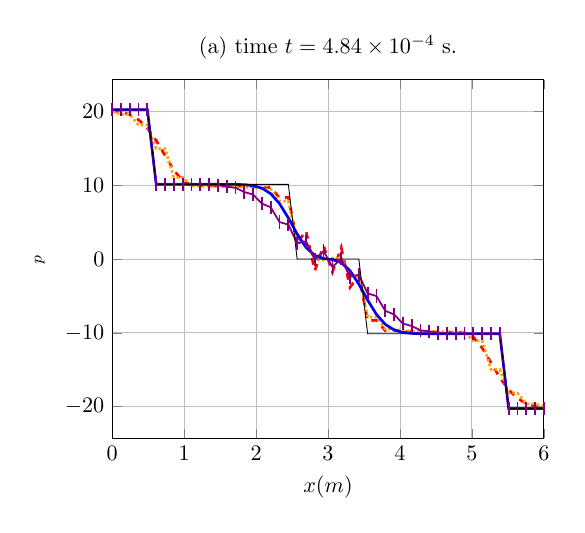
\begin{tikzpicture}[scale=0.8]
\begin{axis}[xlabel=$x (m)$,ylabel=$\eps^p$,ymajorgrids=true,xmajorgrids=true,legend pos=outer north east,title={(a) time $t = 4.84\times 10^{-4} $ s.},xmin=0.,xmax=6.]
\addplot[Red,very thick,mark=none,dashed,mark size=3pt] coordinates {(0.0,20.097963912667037) (0.12244897959183673,19.948200686683876) (0.24489795918367346,19.581623512332886) (0.36734693877551017,18.880401887543975) (0.4897959183673469,17.722027378885375) (0.6122448979591837,16.06462148503811) (0.7346938775510203,14.04922210395701) (0.8571428571428571,12.050777140391757) (0.9795918367346939,10.594448884991046) (1.1020408163265305,10.000299710369095) (1.2244897959183674,9.921016971597252) (1.346938775510204,9.905209334686656) (1.4693877551020407,9.897486036553882) (1.5918367346938775,9.881252793533395) (1.7142857142857142,9.874006895319209) (1.836734693877551,9.827852089496398) (1.9591836734693877,9.84660741015339) (2.0816326530612246,9.635377249359347) (2.204081632653061,9.703660809593103) (2.326530612244898,8.285921376176095) (2.4489795918367347,8.370712342612837) (2.571428571428571,2.1722672846759363) (2.693877551020408,3.830651803002166) (2.816326530612245,-1.5782561078814068) (2.9387755102040813,1.7774061156194738) (3.061224489795918,-1.777406115619491) (3.183673469387755,1.578256107881407) (3.306122448979592,-3.830651803002178) (3.4285714285714284,-2.172267284675949) (3.5510204081632653,-8.370712342612856) (3.673469387755102,-8.285921376176088) (3.7959183673469385,-9.703660809593108) (3.9183673469387754,-9.63537724935935) (4.040816326530612,-9.846607410153386) (4.163265306122449,-9.827852089496393) (4.285714285714286,-9.874006895319202) (4.408163265306122,-9.881252793533392) (4.530612244897959,-9.897486036553879) (4.653061224489796,-9.905209334686653) (4.775510204081632,-9.921016971597266) (4.8979591836734695,-10.000299710369097) (5.020408163265306,-10.594448884991042) (5.142857142857142,-12.05077714039174) (5.26530612244898,-14.049222103957007) (5.387755102040816,-16.064621485038092) (5.5102040816326525,-17.722027378885365) (5.63265306122449,-18.880401887543975) (5.755102040816326,-19.58162351233289) (5.877551020408163,-19.94820068668387) (6.0,-20.09796391266704) };
\addplot[Orange,very thick,mark=none,densely dotted,mark size=3pt] coordinates {(0.0,19.98524356533391) (0.12244897959183673,19.624972673600908) (0.24489795918367346,19.62497267360088) (0.36734693877551017,18.160148281550097) (0.4897959183673469,18.160148281550075) (0.6122448979591837,14.967460990115796) (0.7346938775510203,14.967460990115748) (0.8571428571428571,11.093523181440727) (0.9795918367346939,11.093523181440661) (1.1020408163265305,9.884184161534229) (1.2244897959183674,9.88418416153415) (1.346938775510204,9.848988655347343) (1.4693877551020407,9.848988655347272) (1.5918367346938775,9.805312262992565) (1.7142857142857142,9.805312262992501) (1.836734693877551,9.73354264540347) (1.9591836734693877,9.733542645403414) (2.0816326530612246,9.471881937395924) (2.204081632653061,9.471881937395832) (2.326530612244898,7.860641714627962) (2.4489795918367347,7.860641714627863) (2.571428571428571,2.220437432310992) (2.693877551020408,2.220437432310934) (2.816326530612245,-0.12736436093351383) (2.9387755102040813,-0.1273643609335115) (3.061224489795918,0.12736436093352144) (3.183673469387755,0.12736436093350467) (3.306122448979592,-2.220437432310998) (3.4285714285714284,-2.220437432310941) (3.5510204081632653,-7.860641714628002) (3.673469387755102,-7.860641714627828) (3.7959183673469385,-9.47188193739596) (3.9183673469387754,-9.471881937395791) (4.040816326530612,-9.733542645403523) (4.163265306122449,-9.73354264540336) (4.285714285714286,-9.805312262992585) (4.408163265306122,-9.805312262992468) (4.530612244897959,-9.848988655347373) (4.653061224489796,-9.848988655347233) (4.775510204081632,-9.884184161534241) (4.8979591836734695,-9.884184161534145) (5.020408163265306,-11.093523181440743) (5.142857142857142,-11.093523181440638) (5.26530612244898,-14.967460990115821) (5.387755102040816,-14.967460990115727) (5.5102040816326525,-18.1601482815501) (5.63265306122449,-18.16014828155006) (5.755102040816326,-19.624972673600908) (5.877551020408163,-19.62497267360089) (6.0,-19.985243565333896) };
\addplot[Blue,very thick,mark=none,solid,mark size=3pt] coordinates {(0.0,20.254787341673307) (0.12244897959183673,20.254787341673307) (0.24489795918367346,20.254787341673303) (0.36734693877551017,20.254787341673307) (0.4897959183673469,20.254787341673307) (0.6122448979591837,10.127393670836044) (0.7346938775510203,10.127393670792543) (0.8571428571428571,10.127393669311907) (0.9795918367346939,10.12739363748491) (1.1020408163265305,10.127393152888688) (1.2244897959183674,10.127387597360176) (1.346938775510204,10.127337839606644) (1.4693877551020407,10.1269813177698) (1.5918367346938775,10.124905759760324) (1.7142857142857142,10.114991301522732) (1.836734693877551,10.07592007470102) (1.9591836734693877,9.948669504170498) (2.0816326530612246,9.606755903306565) (2.204081632653061,8.852951991780422) (2.326530612244898,7.502672205682327) (2.4489795918367347,5.567680388456237) (2.571428571428571,3.401350808977297) (2.693877551020408,1.5752238210466734) (2.816326530612245,0.4848507939028141) (2.9387755102040813,0.07365669858902443) (3.061224489795918,-0.07365669858903101) (3.183673469387755,-0.48485079390282165) (3.306122448979592,-1.5752238210466838) (3.4285714285714284,-3.401350808977308) (3.5510204081632653,-5.56768038845625) (3.673469387755102,-7.502672205682339) (3.7959183673469385,-8.852951991780442) (3.9183673469387754,-9.606755903306581) (4.040816326530612,-9.948669504170525) (4.163265306122449,-10.075920074701049) (4.285714285714286,-10.11499130152276) (4.408163265306122,-10.124905759760349) (4.530612244897959,-10.126981317769818) (4.653061224489796,-10.12733783960665) (4.775510204081632,-10.127387597360173) (4.8979591836734695,-10.127393152888683) (5.020408163265306,-10.127393637484907) (5.142857142857142,-10.127393669311903) (5.26530612244898,-10.127393670792548) (5.387755102040816,-10.12739367083605) (5.5102040816326525,-20.25478734167332) (5.63265306122449,-20.254787341673318) (5.755102040816326,-20.25478734167332) (5.877551020408163,-20.25478734167332) (6.0,-20.254787341673314) };
\addplot[Purple,thick,mark=|,solid,mark size=3pt] coordinates {(0.0,20.254787341673307) (0.12244897959183673,20.254787341673307) (0.24489795918367346,20.254787341673303) (0.36734693877551017,20.254787341673307) (0.4897959183673469,20.254787341673307) (0.6122448979591837,10.127346919706891) (0.7346938775510203,10.12727737257173) (0.8571428571428571,10.126334047747402) (0.9795918367346939,10.125114755347433) (1.1020408163265305,10.11630010371687) (1.2244897959183674,10.106478421888186) (1.346938775510204,10.055869021868029) (1.4693877551020407,10.008062509066779) (1.5918367346938775,9.808511707883639) (1.7142857142857142,9.65367054792998) (1.836734693877551,9.082103441085764) (1.9591836734693877,8.739386895433114) (2.0816326530612246,7.513279145883331) (2.204081632653061,7.01727886939908) (2.326530612244898,5.014678544229133) (2.4489795918367347,4.663359241304864) (2.571428571428571,2.1468259041555218) (2.693877551020408,2.417528079544121) (2.816326530612245,-0.05847419216266908) (2.9387755102040813,1.0746179516287027) (3.061224489795918,-1.0746179516287169) (3.183673469387755,0.058474192162660144) (3.306122448979592,-2.417528079544138) (3.4285714285714284,-2.1468259041555355) (3.5510204081632653,-4.663359241304882) (3.673469387755102,-5.014678544229146) (3.7959183673469385,-7.017278869399091) (3.9183673469387754,-7.513279145883345) (4.040816326530612,-8.739386895433125) (4.163265306122449,-9.082103441085776) (4.285714285714286,-9.65367054792999) (4.408163265306122,-9.808511707883648) (4.530612244897959,-10.008062509066782) (4.653061224489796,-10.055869021868036) (4.775510204081632,-10.10647842188818) (4.8979591836734695,-10.11630010371688) (5.020408163265306,-10.125114755347425) (5.142857142857142,-10.12633404774741) (5.26530612244898,-10.127277372571715) (5.387755102040816,-10.127346919706907) (5.5102040816326525,-20.25478734167332) (5.63265306122449,-20.254787341673318) (5.755102040816326,-20.25478734167332) (5.877551020408163,-20.25478734167332) (6.0,-20.254787341673314) };
\addplot[black,thin,mark=none,solid,mark size=3pt] coordinates {(0.0,20.25478734167333) (0.12244897959183673,20.25478734167333) (0.24489795918367346,20.25478734167333) (0.36734693877551017,20.25478734167333) (0.4897959183673469,20.25478734167333) (0.6122448979591837,10.127393670836666) (0.7346938775510203,10.127393670836666) (0.8571428571428571,10.127393670836666) (0.9795918367346939,10.127393670836666) (1.1020408163265305,10.127393670836666) (1.2244897959183674,10.127393670836666) (1.346938775510204,10.127393670836666) (1.4693877551020407,10.127393670836666) (1.5918367346938775,10.127393670836666) (1.7142857142857142,10.127393670836666) (1.836734693877551,10.127393670836666) (1.9591836734693877,10.127393670836666) (2.0816326530612246,10.127393670836666) (2.204081632653061,10.127393670836666) (2.326530612244898,10.127393670836666) (2.4489795918367347,10.127393670836666) (2.571428571428571,-0.0) (2.693877551020408,-0.0) (2.816326530612245,-0.0) (2.9387755102040813,-0.0) (3.061224489795918,-0.0) (3.183673469387755,-0.0) (3.306122448979592,-0.0) (3.4285714285714284,-0.0) (3.5510204081632653,-10.127393670836666) (3.673469387755102,-10.127393670836666) (3.7959183673469385,-10.127393670836666) (3.9183673469387754,-10.127393670836666) (4.040816326530612,-10.127393670836666) (4.163265306122449,-10.127393670836666) (4.285714285714286,-10.127393670836666) (4.408163265306122,-10.127393670836666) (4.530612244897959,-10.127393670836666) (4.653061224489796,-10.127393670836666) (4.775510204081632,-10.127393670836666) (4.8979591836734695,-10.127393670836666) (5.020408163265306,-10.127393670836666) (5.142857142857142,-10.127393670836666) (5.26530612244898,-10.127393670836666) (5.387755102040816,-10.127393670836666) (5.5102040816326525,-20.25478734167333) (5.63265306122449,-20.25478734167333) (5.755102040816326,-20.25478734167333) (5.877551020408163,-20.25478734167333) (6.0,-20.25478734167333) };
%\legend{usl,usf,dgmpm (ep solver),dgmpm (ac solver),exact}
\end{axis}
\end{tikzpicture}
%%% Local Variables:
%%% mode: latex
%%% TeX-master: "../../mainManuscript"
%%% End:
}
  {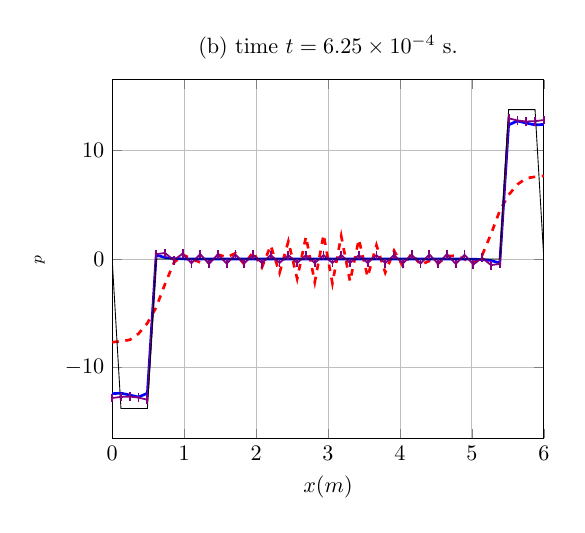
\begin{tikzpicture}[scale=0.8]
\begin{axis}[xlabel=$x (m)$,ylabel=$\eps^p$,ymajorgrids=true,xmajorgrids=true,legend pos=outer north east,title={(b) time $t = 6.25\times 10^{-4} $ s.},xmin=0.,xmax=6.]
\addplot[Red,very thick,mark=none,dashed] coordinates {(0.0,-7.656775715214294) (0.12244897959183673,-7.571339609307247) (0.24489795918367346,-7.438298117574187) (0.36734693877551017,-6.871029176921102) (0.4897959183673469,-5.903192627910385) (0.6122448979591837,-4.452057017543719) (0.7346938775510203,-2.3010481858807137) (0.8571428571428571,-0.3610443561643931) (0.9795918367346939,0.4188880742890505) (1.1020408163265305,0.01523876833598381) (1.2244897959183674,-0.3087249726610329) (1.346938775510204,-0.2682346195141458) (1.4693877551020407,0.41346894641452914) (1.5918367346938775,0.17204334381941044) (1.7142857142857142,0.5321881814826378) (1.836734693877551,-0.5074097815176064) (1.9591836734693877,0.6574508309639426) (2.0816326530612246,-0.7746969731901449) (2.204081632653061,1.2501366726613066) (2.326530612244898,-1.2807853076694733) (2.4489795918367347,1.631639383742251) (2.571428571428571,-1.8095691375383345) (2.693877551020408,2.0564749800644937) (2.816326530612245,-2.129190071354842) (2.9387755102040813,2.240060604992734) (3.061224489795918,-2.240060604992724) (3.183673469387755,2.1291900713548246) (3.306122448979592,-2.0564749800644746) (3.4285714285714284,1.809569137538315) (3.5510204081632653,-1.6316393837422516) (3.673469387755102,1.2807853076694653) (3.7959183673469385,-1.2501366726612742) (3.9183673469387754,0.7746969731901434) (4.040816326530612,-0.657450830963913) (4.163265306122449,0.5074097815175931) (4.285714285714286,-0.5321881814826224) (4.408163265306122,-0.17204334381940892) (4.530612244897959,-0.41346894641450627) (4.653061224489796,0.2682346195141527) (4.775510204081632,0.3087249726610414) (4.8979591836734695,-0.015238768335992692) (5.020408163265306,-0.4188880742890616) (5.142857142857142,0.3610443561643748) (5.26530612244898,2.3010481858807146) (5.387755102040816,4.452057017543711) (5.5102040816326525,5.90319262791038) (5.63265306122449,6.871029176921099) (5.755102040816326,7.4382981175741865) (5.877551020408163,7.571339609307248) (6.0,7.656775715214293) };
\addplot[Blue,very thick,mark=none,solid] coordinates {(0.0,-12.397952325377972) (0.12244897959183673,-12.346999574642966) (0.24489795918367346,-12.523092906128134) (0.36734693877551017,-12.71053547781855) (0.4897959183673469,-12.35049907311499) (0.6122448979591837,0.3722186738331613) (0.7346938775510203,0.1368090990556044) (0.8571428571428571,0.04446044382179651) (0.9795918367346939,0.012779812577704604) (1.1020408163265305,0.0032485856428356346) (1.2244897959183674,0.0007296815528062405) (1.346938775510204,0.00014459919089050038) (1.4693877551020407,2.5219563746036564e-05) (1.5918367346938775,3.857895635058131e-06) (1.7142857142857142,5.15199447901326e-07) (1.836734693877551,5.969388946802084e-08) (1.9591836734693877,5.952534698926585e-09) (2.0816326530612246,5.054662228331333e-10) (2.204081632653061,3.605726635043781e-11) (2.326530612244898,2.127654817367282e-12) (2.4489795918367347,1.1360160010621981e-13) (2.571428571428571,1.3411408617982763e-14) (2.693877551020408,1.66517088668301e-14) (2.816326530612245,5.526766510246074e-15) (2.9387755102040813,6.098792312826054e-15) (3.061224489795918,2.7682726724007426e-15) (3.183673469387755,7.175699018437728e-15) (3.306122448979592,-1.434813028923028e-14) (3.4285714285714284,-8.513769125527232e-15) (3.5510204081632653,-1.0095742773609699e-13) (3.673469387755102,-2.1199430888032018e-12) (3.7959183673469385,-3.6039619852103143e-11) (3.9183673469387754,-5.0545241703127e-10) (4.040816326530612,-5.9525221489037014e-09) (4.163265306122449,-5.969386814802888e-08) (4.285714285714286,-5.151994230605103e-07) (4.408163265306122,-3.8578956228878976e-06) (4.530612244897959,-2.5219563737562718e-05) (4.653061224489796,-0.00014459919087944834) (4.775510204081632,-0.0007296815527927886) (4.8979591836734695,-0.0032485856428289012) (5.020408163265306,-0.012779812577696097) (5.142857142857142,-0.04446044382178102) (5.26530612244898,-0.13680909905559333) (5.387755102040816,-0.3722186738331447) (5.5102040816326525,12.350499073115015) (5.63265306122449,12.71053547781857) (5.755102040816326,12.523092906128156) (5.877551020408163,12.346999574642979) (6.0,12.39795232537799) };
\addplot[Purple,thick,mark=|,solid] coordinates {(0.0,-12.795628373535159) (0.12244897959183673,-12.695543273778933) (0.24489795918367346,-12.666110940711564) (0.36734693877551017,-12.75241410003132) (0.4897959183673469,-12.960739789752774) (0.6122448979591837,0.44192323057668886) (0.7346938775510203,0.5605175207125453) (0.8571428571428571,-0.1118177278404644) (0.9795918367346939,0.49857571480888807) (1.1020408163265305,-0.3912177295445921) (1.2244897959183674,0.45869222504142426) (1.346938775510204,-0.4542184988816014) (1.4693877551020407,0.4392500135640788) (1.5918367346938775,-0.4268192827562814) (1.7142857142857142,0.4185270888397142) (1.836734693877551,-0.39693938041336063) (1.9591836734693877,0.398295251539175) (2.0816326530612246,-0.37211426798041747) (2.204081632653061,0.37593537352436907) (2.326530612244898,-0.3607380778681954) (2.4489795918367347,0.36132221537101705) (2.571428571428571,-0.3654682237983432) (2.693877551020408,0.35826901292698654) (2.816326530612245,-0.3691156051231741) (2.9387755102040813,0.36040411668068795) (3.061224489795918,-0.3604041166806867) (3.183673469387755,0.369115605123182) (3.306122448979592,-0.3582690129270081) (3.4285714285714284,0.36546822379836186) (3.5510204081632653,-0.3613222153709926) (3.673469387755102,0.3607380778681742) (3.7959183673469385,-0.37593537352436845) (3.9183673469387754,0.37211426798044456) (4.040816326530612,-0.3982952515391655) (4.163265306122449,0.3969393804133886) (4.285714285714286,-0.4185270888397233) (4.408163265306122,0.42681928275629366) (4.530612244897959,-0.43925001356404864) (4.653061224489796,0.45421849888160465) (4.775510204081632,-0.4586922250414254) (4.8979591836734695,0.3912177295446241) (5.020408163265306,-0.4985757148088702) (5.142857142857142,0.11181772784050628) (5.26530612244898,-0.560517520712548) (5.387755102040816,-0.4419232305766629) (5.5102040816326525,12.960739789752816) (5.63265306122449,12.75241410003134) (5.755102040816326,12.666110940711583) (5.877551020408163,12.695543273778958) (6.0,12.795628373535196) };
\addplot[black,thin,mark=none,solid] coordinates {(0.0,-0.0) (0.12244897959183673,-13.758687910475539) (0.24489795918367346,-13.758687910475539) (0.36734693877551017,-13.758687910475539) (0.4897959183673469,-13.758687910475539) (0.6122448979591837,-0.0) (0.7346938775510203,-0.0) (0.8571428571428571,-0.0) (0.9795918367346939,-0.0) (1.1020408163265305,-0.0) (1.2244897959183674,-0.0) (1.346938775510204,-0.0) (1.4693877551020407,-0.0) (1.5918367346938775,-0.0) (1.7142857142857142,-0.0) (1.836734693877551,-0.0) (1.9591836734693877,-0.0) (2.0816326530612246,-0.0) (2.204081632653061,-0.0) (2.326530612244898,-0.0) (2.4489795918367347,-0.0) (2.571428571428571,-0.0) (2.693877551020408,-0.0) (2.816326530612245,-0.0) (2.9387755102040813,-0.0) (3.061224489795918,-0.0) (3.183673469387755,-0.0) (3.306122448979592,-0.0) (3.4285714285714284,-0.0) (3.5510204081632653,-0.0) (3.673469387755102,-0.0) (3.7959183673469385,-0.0) (3.9183673469387754,-0.0) (4.040816326530612,-0.0) (4.163265306122449,-0.0) (4.285714285714286,-0.0) (4.408163265306122,-0.0) (4.530612244897959,-0.0) (4.653061224489796,-0.0) (4.775510204081632,-0.0) (4.8979591836734695,-0.0) (5.020408163265306,-0.0) (5.142857142857142,-0.0) (5.26530612244898,-0.0) (5.387755102040816,-0.0) (5.5102040816326525,13.758687910475539) (5.63265306122449,13.758687910475539) (5.755102040816326,13.758687910475539) (5.877551020408163,13.758687910475539) (6.0,0.0) };
%\legend{usl 1ppc,dgmpm 1ppc (ep solver),dgmpm 1ppc (ac solver),exact}
\end{axis}
\end{tikzpicture}
%%% Local Variables:
%%% mode: latex
%%% TeX-master: "../../mainManuscript"
%%% End:
}
  {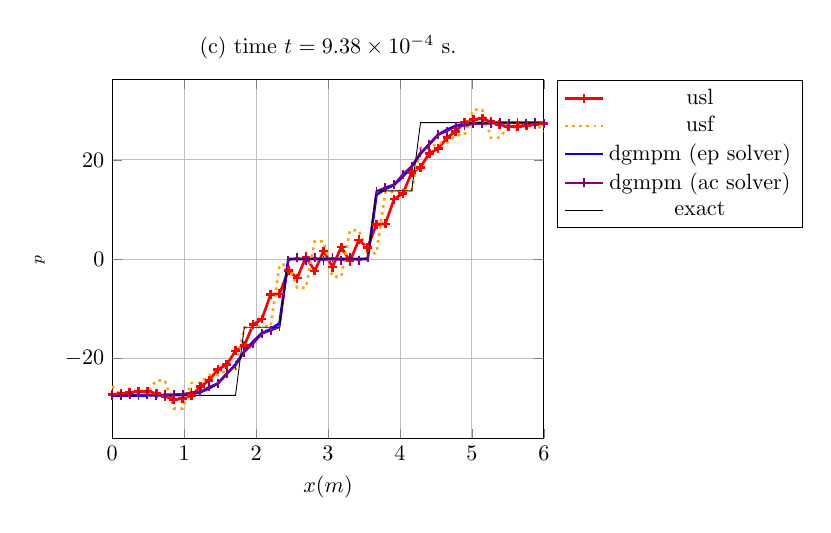
\begin{tikzpicture}[scale=0.8]
\begin{axis}[xlabel=$x (m)$,ylabel=$\eps^p$,ymajorgrids=true,xmajorgrids=true,legend pos=outer north east,title={(c) time $t = 9.38\times 10^{-4} $ s.},xmin=0.,xmax=6.]
\addplot[Red,very thick,mark=+,solid] coordinates {(0.0,-27.331872449853556) (0.12244897959183673,-27.174400085417467) (0.24489795918367346,-26.904779830121768) (0.36734693877551017,-26.69301343005911) (0.4897959183673469,-26.683543140751915) (0.6122448979591837,-27.106963962300345) (0.7346938775510203,-27.704030887608354) (0.8571428571428571,-28.33906014232905) (0.9795918367346939,-28.167172814076366) (1.1020408163265305,-27.53334986092529) (1.2244897959183674,-25.775044707062726) (1.346938775510204,-24.466615882102165) (1.4693877551020407,-22.247186500301964) (1.5918367346938775,-21.33079179039491) (1.7142857142857142,-18.523714044368063) (1.836734693877551,-17.44233776410034) (1.9591836734693877,-13.237799741628182) (2.0816326530612246,-12.0894356407598) (2.204081632653061,-7.096371776087362) (2.326530612244898,-7.032925295785245) (2.4489795918367347,-2.2620897664972315) (2.571428571428571,-3.858668388515009) (2.693877551020408,0.4300541105363164) (2.816326530612245,-2.410115988529146) (2.9387755102040813,1.6326922086221445) (3.061224489795918,-1.6326922086221325) (3.183673469387755,2.410115988529122) (3.306122448979592,-0.43005411053631265) (3.4285714285714284,3.858668388514974) (3.5510204081632653,2.2620897664972395) (3.673469387755102,7.032925295785231) (3.7959183673469385,7.096371776087392) (3.9183673469387754,12.089435640759786) (4.040816326530612,13.237799741628214) (4.163265306122449,17.442337764100337) (4.285714285714286,18.523714044368088) (4.408163265306122,21.330791790394894) (4.530612244897959,22.247186500301982) (4.653061224489796,24.466615882102147) (4.775510204081632,25.775044707062744) (4.8979591836734695,27.53334986092529) (5.020408163265306,28.167172814076363) (5.142857142857142,28.33906014232903) (5.26530612244898,27.70403088760834) (5.387755102040816,27.106963962300348) (5.5102040816326525,26.683543140751933) (5.63265306122449,26.693013430059132) (5.755102040816326,26.904779830121797) (5.877551020408163,27.17440008541749) (6.0,27.331872449853574) };
\addplot[Orange,very thick,mark=none,dotted] coordinates {(0.0,-25.658312786761723) (0.12244897959183673,-27.51413969235028) (0.24489795918367346,-27.514139692350327) (0.36734693877551017,-26.86847994686687) (0.4897959183673469,-26.868479946866948) (0.6122448979591837,-24.492978695040286) (0.7346938775510203,-24.49297869504042) (0.8571428571428571,-30.15019249346318) (0.9795918367346939,-30.15019249346324) (1.1020408163265305,-24.98956773450457) (1.2244897959183674,-24.98956773450463) (1.346938775510204,-23.40942037125753) (1.4693877551020407,-23.409420371257625) (1.5918367346938775,-22.418334622056513) (1.7142857142857142,-22.418334622056435) (1.836734693877551,-13.85468254978275) (1.9591836734693877,-13.854682549782833) (2.0816326530612246,-13.574506608280911) (2.204081632653061,-13.574506608280759) (2.326530612244898,-1.1520841431514552) (2.4489795918367347,-1.1520841431514355) (2.571428571428571,-5.798608057459956) (2.693877551020408,-5.7986080574598535) (2.816326530612245,3.5614225712693863) (2.9387755102040813,3.5614225712696768) (3.061224489795918,-3.5614225712695777) (3.183673469387755,-3.561422571269489) (3.306122448979592,5.798608057459823) (3.4285714285714284,5.798608057459984) (3.5510204081632653,1.1520841431513575) (3.673469387755102,1.152084143151603) (3.7959183673469385,13.574506608280872) (3.9183673469387754,13.574506608280805) (4.040816326530612,13.854682549782702) (4.163265306122449,13.854682549782932) (4.285714285714286,22.418334622056502) (4.408163265306122,22.418334622056456) (4.530612244897959,23.409420371257596) (4.653061224489796,23.40942037125754) (4.775510204081632,24.989567734504483) (4.8979591836734695,24.98956773450469) (5.020408163265306,30.150192493463102) (5.142857142857142,30.15019249346332) (5.26530612244898,24.49297869504033) (5.387755102040816,24.492978695040364) (5.5102040816326525,26.868479946866863) (5.63265306122449,26.86847994686695) (5.755102040816326,27.51413969235029) (5.877551020408163,27.51413969235035) (6.0,25.65831278676172) };
\addplot[Blue,very thick,mark=none,solid] coordinates {(0.0,-27.517363397075158) (0.12244897959183673,-27.51732379155038) (0.24489795918367346,-27.517228936294842) (0.36734693877551017,-27.516689788484122) (0.4897959183673469,-27.51556852970287) (0.6122448979591837,-27.51025382248486) (0.7346938775510203,-27.500198710367762) (0.8571428571428571,-27.46081288016468) (0.9795918367346939,-27.394149463815683) (1.1020408163265305,-27.182111927326957) (1.2244897959183674,-26.86831399158136) (1.346938775510204,-26.078149290066197) (1.4693877551020407,-25.088393528723113) (1.5918367346938775,-23.18951900040588) (1.7142857142857142,-21.27348955232938) (1.836734693877551,-18.64183859399964) (1.9591836734693877,-16.674856395188144) (2.0816326530612246,-14.952075198356093) (2.204081632653061,-14.149762008703409) (2.326530612244898,-12.97119731020455) (2.4489795918367347,1.4749921389468362e-14) (2.571428571428571,2.901956841536459e-14) (2.693877551020408,2.1854428799290698e-14) (2.816326530612245,2.1134926307627894e-14) (2.9387755102040813,2.170695211020788e-14) (3.061224489795918,2.3579152402243164e-14) (3.183673469387755,1.2378418950898343e-14) (3.306122448979592,1.1665469373072734e-14) (3.4285714285714284,7.094390671854583e-15) (3.5510204081632653,8.299690845575712e-15) (3.673469387755102,12.971197310204621) (3.7959183673469385,14.149762008703473) (3.9183673469387754,14.952075198356113) (4.040816326530612,16.674856395188158) (4.163265306122449,18.641838593999683) (4.285714285714286,21.273489552329384) (4.408163265306122,23.189519000405888) (4.530612244897959,25.088393528723138) (4.653061224489796,26.07814929006618) (4.775510204081632,26.868313991581342) (4.8979591836734695,27.182111927326957) (5.020408163265306,27.3941494638157) (5.142857142857142,27.46081288016466) (5.26530612244898,27.500198710367762) (5.387755102040816,27.51025382248485) (5.5102040816326525,27.515568529702865) (5.63265306122449,27.51668978848415) (5.755102040816326,27.517228936294806) (5.877551020408163,27.517323791550382) (6.0,27.517363397075165) };
\addplot[Purple,thick,mark=|,solid] coordinates {(0.0,-27.455491898583844) (0.12244897959183673,-27.52990791746212) (0.24489795918367346,-27.39669410111553) (0.36734693877551017,-27.56069772218648) (0.4897959183673469,-27.354208534961813) (0.6122448979591837,-27.484169218141297) (0.7346938775510203,-27.30529154707286) (0.8571428571428571,-27.260887430891447) (0.9795918367346939,-27.234362200737557) (1.1020408163265305,-26.87048565463221) (1.2244897959183674,-26.76603983934888) (1.346938775510204,-25.75807449243556) (1.4693877551020407,-25.06955937174821) (1.5918367346938775,-23.02673771458467) (1.7142857142857142,-21.509235536573875) (1.836734693877551,-18.773874989550777) (1.9591836734693877,-17.141311478227397) (2.0816326530612246,-15.098912535609557) (2.204081632653061,-14.451161421148855) (2.326530612244898,-13.715612700621918) (2.4489795918367347,-0.23693029878140853) (2.571428571428571,0.24220658661539068) (2.693877551020408,-0.22882318056987147) (2.816326530612245,0.2316928153217551) (2.9387755102040813,-0.22713962166300733) (3.061224489795918,0.22713962166305024) (3.183673469387755,-0.2316928153217785) (3.306122448979592,0.22882318056992768) (3.4285714285714284,-0.24220658661539307) (3.5510204081632653,0.23693029878141705) (3.673469387755102,13.71561270062201) (3.7959183673469385,14.451161421148875) (3.9183673469387754,15.098912535609603) (4.040816326530612,17.141311478227408) (4.163265306122449,18.77387498955077) (4.285714285714286,21.509235536573904) (4.408163265306122,23.026737714584694) (4.530612244897959,25.06955937174818) (4.653061224489796,25.758074492435522) (4.775510204081632,26.766039839348913) (4.8979591836734695,26.870485654632194) (5.020408163265306,27.23436220073757) (5.142857142857142,27.260887430891422) (5.26530612244898,27.305291547072898) (5.387755102040816,27.484169218141297) (5.5102040816326525,27.354208534961796) (5.63265306122449,27.560697722186475) (5.755102040816326,27.39669410111557) (5.877551020408163,27.529907917462097) (6.0,27.455491898583855) };
\addplot[black,thin,mark=none,solid] coordinates {(0.0,-27.517375820951077) (0.12244897959183673,-27.517375820951077) (0.24489795918367346,-27.517375820951077) (0.36734693877551017,-27.517375820951077) (0.4897959183673469,-27.517375820951077) (0.6122448979591837,-27.517375820951077) (0.7346938775510203,-27.517375820951077) (0.8571428571428571,-27.517375820951077) (0.9795918367346939,-27.517375820951077) (1.1020408163265305,-27.517375820951077) (1.2244897959183674,-27.517375820951077) (1.346938775510204,-27.517375820951077) (1.4693877551020407,-27.517375820951077) (1.5918367346938775,-27.517375820951077) (1.7142857142857142,-27.517375820951077) (1.836734693877551,-13.758687910475539) (1.9591836734693877,-13.758687910475539) (2.0816326530612246,-13.758687910475539) (2.204081632653061,-13.758687910475539) (2.326530612244898,-13.758687910475539) (2.4489795918367347,-0.0) (2.571428571428571,-0.0) (2.693877551020408,-0.0) (2.816326530612245,-0.0) (2.9387755102040813,-0.0) (3.061224489795918,-0.0) (3.183673469387755,-0.0) (3.306122448979592,-0.0) (3.4285714285714284,-0.0) (3.5510204081632653,-0.0) (3.673469387755102,13.758687910475539) (3.7959183673469385,13.758687910475539) (3.9183673469387754,13.758687910475539) (4.040816326530612,13.758687910475539) (4.163265306122449,13.758687910475539) (4.285714285714286,27.517375820951077) (4.408163265306122,27.517375820951077) (4.530612244897959,27.517375820951077) (4.653061224489796,27.517375820951077) (4.775510204081632,27.517375820951077) (4.8979591836734695,27.517375820951077) (5.020408163265306,27.517375820951077) (5.142857142857142,27.517375820951077) (5.26530612244898,27.517375820951077) (5.387755102040816,27.517375820951077) (5.5102040816326525,27.517375820951077) (5.63265306122449,27.517375820951077) (5.755102040816326,27.517375820951077) (5.877551020408163,27.517375820951077) (6.0,27.517375820951077) };
\legend{usl,usf,dgmpm (ep solver),dgmpm (ac solver),exact}
\end{axis}
\end{tikzpicture}
%%% Local Variables:
%%% mode: latex
%%% TeX-master: "../../mainManuscript"
%%% End:
}
  \caption{elastic-plastic RP velo}
  \label{fig:velo_elastoplastic_RP}
\end{figure}
Comparison with mpm for 1ppc and 2ppcs with RK2
\begin{figure}[h!]
  \centering
  {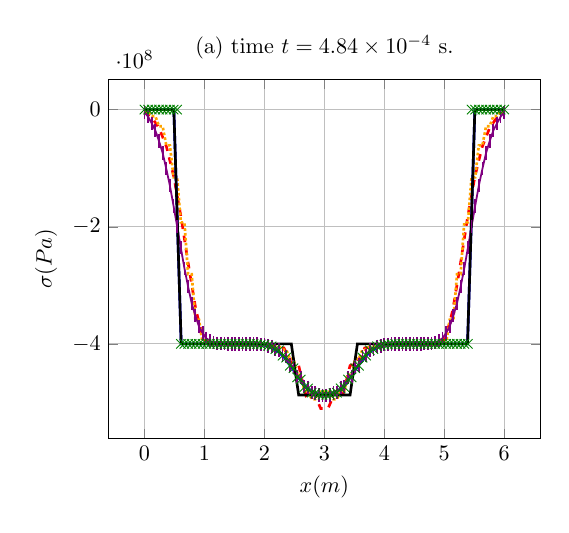
\begin{tikzpicture}[scale=0.8]
\begin{axis}[xlabel=$x (m)$,ylabel=$\sigma (Pa)$,ymajorgrids=true,xmajorgrids=true,legend pos=outer north east,title={(a) time $t = 4.84\times 10^{-4} $ s.}]
\addplot[Red,very thick,mark=none,dashed,mark size=3pt] coordinates {(0.0,-3669561.908091424) (0.12244897959183673,-13594450.379485756) (0.24489795918367346,-31624435.10565728) (0.36734693877551017,-63707048.32128755) (0.4897959183673469,-114660806.5675256) (0.6122448979591837,-184794660.6509606) (0.7346938775510203,-266179173.63903272) (0.8571428571428571,-341775310.1478163) (0.9795918367346939,-390693099.4776282) (1.1020408163265305,-400379159.02115166) (1.2244897959183674,-400770866.2752631) (1.346938775510204,-400849758.67078286) (1.4693877551020407,-400903087.2437715) (1.5918367346938775,-400974206.0457186) (1.7142857142857142,-401177729.4632526) (1.836734693877551,-401187799.71208847) (1.9591836734693877,-401722959.3911894) (2.0816326530612246,-401625095.9277148) (2.204081632653061,-405721718.460188) (2.326530612244898,-406980928.2270958) (2.4489795918367347,-432556847.70391244) (2.571428571428571,-437038541.50331527) (2.693877551020408,-488555362.3021708) (2.816326530612245,-481341619.82050365) (2.9387755102040813,-510307309.7388937) (3.061224489795918,-510307309.7388923) (3.183673469387755,-481341619.8205054) (3.306122448979592,-488555362.3021694) (3.4285714285714284,-437038541.50331557) (3.5510204081632653,-432556847.70391184) (3.673469387755102,-406980928.2270957) (3.7959183673469385,-405721718.4601879) (3.9183673469387754,-401625095.9277147) (4.040816326530612,-401722959.3911895) (4.163265306122449,-401187799.71208847) (4.285714285714286,-401177729.4632526) (4.408163265306122,-400974206.0457186) (4.530612244897959,-400903087.2437715) (4.653061224489796,-400849758.670783) (4.775510204081632,-400770866.2752632) (4.8979591836734695,-400379159.02115154) (5.020408163265306,-390693099.47762805) (5.142857142857142,-341775310.1478161) (5.26530612244898,-266179173.63903314) (5.387755102040816,-184794660.65096068) (5.5102040816326525,-114660806.56752594) (5.63265306122449,-63707048.32128816) (5.755102040816326,-31624435.10565742) (5.877551020408163,-13594450.3794861) (6.0,-3669561.9080915614) };
\addplot[Orange,very thick,mark=none,densely dotted,mark size=3pt] coordinates {(0.0,-2914267.3201301154) (0.06060606060606061,-2914267.3201301154) (0.12121212121212122,-11378318.451142035) (0.18181818181818182,-11378318.451142035) (0.24242424242424243,-28406466.993262846) (0.30303030303030304,-28406466.993262846) (0.36363636363636365,-61055835.593559496) (0.42424242424242425,-61055835.593559496) (0.48484848484848486,-115583582.76704544) (0.5454545454545454,-115583582.76704544) (0.6060606060606061,-192564241.19110337) (0.6666666666666667,-192564241.19110337) (0.7272727272727273,-281227079.2224079) (0.7878787878787878,-281227079.2224079) (0.8484848484848485,-358622783.83691025) (0.9090909090909092,-358622783.83691025) (0.9696969696969697,-399584151.64208454) (1.0303030303030303,-399584151.64208454) (1.0909090909090908,-400518950.3403047) (1.1515151515151516,-400518950.3403047) (1.2121212121212122,-400764480.1267914) (1.2727272727272727,-400764480.1267914) (1.3333333333333335,-400835508.12332404) (1.393939393939394,-400835508.12332404) (1.4545454545454546,-400891006.2882111) (1.5151515151515151,-400891006.2882111) (1.5757575757575757,-400939762.1508219) (1.6363636363636365,-400939762.1508219) (1.696969696969697,-401049302.5008664) (1.7575757575757576,-401049302.5008664) (1.8181818181818183,-401273466.6129426) (1.878787878787879,-401273466.6129426) (1.9393939393939394,-401521516.00275475) (2.0,-401521516.00275475) (2.0606060606060606,-402092208.5638283) (2.121212121212121,-402092208.5638283) (2.1818181818181817,-404027519.3843328) (2.2424242424242427,-404027519.3843328) (2.303030303030303,-409750544.23386204) (2.3636363636363638,-409750544.23386204) (2.4242424242424243,-425145499.736588) (2.484848484848485,-425145499.736588) (2.5454545454545454,-452445709.1416535) (2.606060606060606,-452445709.1416535) (2.666666666666667,-479926155.3868412) (2.7272727272727275,-479926155.3868412) (2.787878787878788,-494460484.088121) (2.8484848484848486,-494460484.088121) (2.909090909090909,-481596066.8615678) (2.9696969696969697,-481596066.8615678) (3.0303030303030303,-481596066.8615678) (3.090909090909091,-481596066.8615678) (3.1515151515151514,-494460484.088121) (3.2121212121212124,-494460484.088121) (3.272727272727273,-479926155.3868412) (3.3333333333333335,-479926155.3868412) (3.393939393939394,-452445709.1416535) (3.4545454545454546,-452445709.1416535) (3.515151515151515,-425145499.736588) (3.5757575757575757,-425145499.736588) (3.6363636363636367,-409750544.23386204) (3.6969696969696972,-409750544.23386204) (3.757575757575758,-404027519.3843328) (3.8181818181818183,-404027519.3843328) (3.878787878787879,-402092208.5638283) (3.9393939393939394,-402092208.5638283) (4.0,-401521516.0027547) (4.0606060606060606,-401521516.0027547) (4.121212121212121,-401273466.6129426) (4.181818181818182,-401273466.6129426) (4.242424242424242,-401049302.5008665) (4.303030303030303,-401049302.5008665) (4.363636363636363,-400939762.15082186) (4.424242424242425,-400939762.15082186) (4.484848484848485,-400891006.2882111) (4.545454545454546,-400891006.2882111) (4.606060606060606,-400835508.12332404) (4.666666666666667,-400835508.12332404) (4.7272727272727275,-400764480.1267914) (4.787878787878788,-400764480.1267914) (4.848484848484849,-400518950.3403046) (4.909090909090909,-400518950.3403046) (4.96969696969697,-399584151.6420844) (5.03030303030303,-399584151.6420844) (5.090909090909091,-358622783.8369101) (5.151515151515151,-358622783.8369101) (5.212121212121212,-281227079.22240764) (5.2727272727272725,-281227079.22240764) (5.333333333333334,-192564241.19110358) (5.3939393939393945,-192564241.19110358) (5.454545454545455,-115583582.76704524) (5.515151515151516,-115583582.76704524) (5.575757575757576,-61055835.59355964) (5.636363636363637,-61055835.59355964) (5.696969696969697,-28406466.99326251) (5.757575757575758,-28406466.99326251) (5.818181818181818,-11378318.451142171) (5.878787878787879,-11378318.451142171) (5.9393939393939394,-2914267.3201301834) (6.0,-2914267.3201301834) };
\addplot[Blue,very thick,mark=none,solid,mark size=3pt] coordinates {(0.0,-1.4032094709741823e-07) (0.12244897959183673,1.4032094709741797e-07) (0.24489795918367346,-5.501313561848306e-23) (0.36734693877551017,-1.4032094709741882e-07) (0.4897959183673469,-4.2096284129225576e-07) (0.6122448979591837,-400000000.0000052) (0.7346938775510203,-400000000.0003803) (0.8571428571428571,-400000000.0131417) (0.9795918367346939,-400000000.2874559) (1.1020408163265305,-400000004.46415013) (1.2244897959183674,-400000052.34678423) (1.346938775510204,-400000481.2046858) (1.4693877551020407,-400003554.03647596) (1.5918367346938775,-400021443.0967657) (1.7142857142857142,-400106894.9802318) (1.836734693877551,-400443646.6051052) (1.9591836734693877,-401540408.59283984) (2.0816326530612246,-404487333.2231472) (2.204081632653061,-410984305.87262785) (2.326530612244898,-422622254.02503896) (2.4489795918367347,-439299786.1010327) (2.571428571428571,-457971198.93456453) (2.693877551020408,-473710434.18348145) (2.816326530612245,-483108267.7934754) (2.9387755102040813,-486652315.1909913) (3.061224489795918,-486652315.1909913) (3.183673469387755,-483108267.7934754) (3.306122448979592,-473710434.18348145) (3.4285714285714284,-457971198.93456453) (3.5510204081632653,-439299786.1010328) (3.673469387755102,-422622254.025039) (3.7959183673469385,-410984305.8726279) (3.9183673469387754,-404487333.2231472) (4.040816326530612,-401540408.59283984) (4.163265306122449,-400443646.6051051) (4.285714285714286,-400106894.98023176) (4.408163265306122,-400021443.0967656) (4.530612244897959,-400003554.0364758) (4.653061224489796,-400000481.20468575) (4.775510204081632,-400000052.3467841) (4.8979591836734695,-400000004.46415013) (5.020408163265306,-400000000.2874559) (5.142857142857142,-400000000.01314175) (5.26530612244898,-400000000.0003803) (5.387755102040816,-400000000.0000052) (5.5102040816326525,1.403209470974181e-07) (5.63265306122449,-4.209628412922546e-07) (5.755102040816326,-7.335084749131074e-23) (5.877551020408163,-7.335084749131074e-23) (6.0,1.4032094709741816e-07) };
\addplot[Purple,thick,mark=|,solid,mark size=3pt] coordinates {(0.0,-4432924.706841537) (0.06060606060606061,-12207367.937325412) (0.12121212121212122,-23531843.32279323) (0.18181818181818182,-35734156.38126936) (0.24242424242424243,-53819967.0341102) (0.30303030303030304,-73960503.34391399) (0.36363636363636365,-100971777.07395627) (0.42424242424242425,-130109924.83030084) (0.48484848484848486,-164461120.69762146) (0.5454545454545454,-199783681.59143203) (0.6060606060606061,-235957589.20194656) (0.6666666666666667,-271228096.10690445) (0.7272727272727273,-302213993.4219046) (0.7878787878787878,-330771054.2743039) (0.8484848484848485,-351899554.770462) (0.9090909090909092,-370258280.79493797) (0.9696969696969697,-381361519.41978526) (1.0303030303030303,-390443246.24646133) (1.0909090909090908,-394697061.64063984) (1.1515151515151516,-397978403.46801) (1.2121212121212122,-399033797.91006035) (1.2727272727272727,-399815009.1781527) (1.3333333333333335,-399928549.7385389) (1.393939393939394,-400001024.16277933) (1.4545454545454546,-400002181.8139095) (1.5151515151515151,-400003409.2713153) (1.5757575757575757,-400013260.9517136) (1.6363636363636365,-400019327.12601054) (1.696969696969697,-400071982.9779926) (1.7575757575757576,-400098745.1685716) (1.8181818181818183,-400318321.7394188) (1.878787878787879,-400414890.0391485) (1.9393939393939394,-401165297.85083073) (2.0,-401450756.0252169) (2.0606060606060606,-403565545.76565593) (2.121212121212121,-404257062.9865757) (2.1818181818181817,-409162020.12612975) (2.2424242424242427,-410524033.8850246) (2.303030303030303,-419802201.6406596) (2.3636363636363638,-421949146.8716409) (2.4242424242424243,-436028496.5842672) (2.484848484848485,-438667957.45895886) (2.5454545454545454,-455363332.4481878) (2.606060606060606,-457791067.839726) (2.666666666666667,-472627847.3837442) (2.7272727272727275,-474182129.162814) (2.787878787878788,-483383494.6652765) (2.8484848484848486,-483980615.0668598) (2.909090909090909,-487493210.5310644) (2.9696969696969697,-487590657.9314887) (3.0303030303030303,-487590657.9314887) (3.090909090909091,-487493210.5310644) (3.1515151515151514,-483980615.0668598) (3.2121212121212124,-483383494.6652765) (3.272727272727273,-474182129.162814) (3.3333333333333335,-472627847.38374436) (3.393939393939394,-457791067.839726) (3.4545454545454546,-455363332.4481878) (3.515151515151515,-438667957.458959) (3.5757575757575757,-436028496.5842673) (3.6363636363636367,-421949146.871641) (3.6969696969696972,-419802201.6406597) (3.757575757575758,-410524033.8850248) (3.8181818181818183,-409162020.1261299) (3.878787878787879,-404257062.98657584) (3.9393939393939394,-403565545.765656) (4.0,-401450756.0252169) (4.0606060606060606,-401165297.85083085) (4.121212121212121,-400414890.0391486) (4.181818181818182,-400318321.7394188) (4.242424242424242,-400098745.1685716) (4.303030303030303,-400071982.9779927) (4.363636363636363,-400019327.12601066) (4.424242424242425,-400013260.95171374) (4.484848484848485,-400003409.2713153) (4.545454545454546,-400002181.8139095) (4.606060606060606,-400001024.16277933) (4.666666666666667,-399928549.7385392) (4.7272727272727275,-399815009.17815316) (4.787878787878788,-399033797.9100607) (4.848484848484849,-397978403.46801054) (4.909090909090909,-394697061.6406404) (4.96969696969697,-390443246.24646163) (5.03030303030303,-381361519.4197858) (5.090909090909091,-370258280.7949385) (5.151515151515151,-351899554.7704626) (5.212121212121212,-330771054.27430445) (5.2727272727272725,-302213993.42190534) (5.333333333333334,-271228096.1069048) (5.3939393939393945,-235957589.201947) (5.454545454545455,-199783681.5914322) (5.515151515151516,-164461120.6976217) (5.575757575757576,-130109924.83030085) (5.636363636363637,-100971777.07395627) (5.696969696969697,-73960503.34391414) (5.757575757575758,-53819967.034110345) (5.818181818181818,-35734156.38126946) (5.878787878787879,-23531843.322793126) (5.9393939393939394,-12207367.937325357) (6.0,-4432924.706841591) };
\addplot[Green,thin,mark=x,only marks,mark size=3pt] coordinates {(0.0,1.2652173515404603e-06) (0.06060606060606061,9.799178020182319e-07) (0.12121212121212122,-4.084567774230407e-07) (0.18181818181818182,-4.3346890516146844e-07) (0.24242424242424243,4.563473356624432e-07) (0.30303030303030304,3.855783469220664e-07) (0.36363636363636365,-5.846850939002003e-07) (0.42424242424242425,-8.185243770739822e-07) (0.48484848484848486,5.883985548618523e-07) (0.5454545454545454,8.148109161123314e-07) (0.6060606060606061,-400000000.0000001) (0.6666666666666667,-400000000.0000003) (0.7272727272727273,-400000000.00001395) (0.7878787878787878,-400000000.0000309) (0.8484848484848485,-400000000.0007001) (0.9090909090909092,-400000000.0014903) (0.9696969696969697,-400000000.0219135) (1.0303030303030303,-400000000.0446493) (1.0909090909090908,-400000000.4778095) (1.1515151515151516,-400000000.93062043) (1.2121212121212122,-400000007.7115201) (1.2727272727272727,-400000014.3371707) (1.3333333333333335,-400000095.54857785) (1.393939393939394,-400000169.3314061) (1.4545454545454546,-400000930.466908) (1.5151515151515151,-400001569.6122349) (1.5757575757575757,-400007232.7377954) (1.6363636363636365,-400011597.9099656) (1.696969696969697,-400045337.5232003) (1.7575757575757576,-400069019.1005317) (1.8181818181818183,-400230656.1994125) (1.878787878787879,-400332993.2150553) (1.9393939393939394,-400955956.96957076) (2.0,-401307731.2616477) (2.0606060606060606,-403233382.7711176) (2.121212121212121,-404189912.7567165) (2.1818181818181817,-408931765.9664936) (2.2424242424242427,-410968365.8644036) (2.303030303030303,-420167583.50623786) (2.3636363636363638,-423508767.0960166) (2.4242424242424243,-437335267.865692) (2.484848484848485,-441457068.1017972) (2.5454545454545454,-457161702.9599444) (2.606060606060606,-460844115.7211842) (2.666666666666667,-473822399.01136905) (2.7272727272727275,-476062326.4885395) (2.787878787878788,-483396938.4157252) (2.8484848484848486,-484223655.8917301) (2.909090909090909,-486749500.07510275) (2.9696969696969697,-486888696.01046515) (3.0303030303030303,-486888696.01046515) (3.090909090909091,-486749500.07510275) (3.1515151515151514,-484223655.8917301) (3.2121212121212124,-483396938.4157252) (3.272727272727273,-476062326.4885395) (3.3333333333333335,-473822399.0113689) (3.393939393939394,-460844115.721184) (3.4545454545454546,-457161702.9599444) (3.515151515151515,-441457068.1017974) (3.5757575757575757,-437335267.865692) (3.6363636363636367,-423508767.0960167) (3.6969696969696972,-420167583.506238) (3.757575757575758,-410968365.8644036) (3.8181818181818183,-408931765.9664936) (3.878787878787879,-404189912.7567166) (3.9393939393939394,-403233382.7711176) (4.0,-401307731.2616477) (4.0606060606060606,-400955956.9695708) (4.121212121212121,-400332993.2150553) (4.181818181818182,-400230656.1994125) (4.242424242424242,-400069019.1005317) (4.303030303030303,-400045337.5232003) (4.363636363636363,-400011597.9099656) (4.424242424242425,-400007232.7377954) (4.484848484848485,-400001569.6122349) (4.545454545454546,-400000930.466908) (4.606060606060606,-400000169.3314062) (4.666666666666667,-400000095.5485779) (4.7272727272727275,-400000014.3371707) (4.787878787878788,-400000007.7115201) (4.848484848484849,-400000000.93062043) (4.909090909090909,-400000000.4778095) (4.96969696969697,-400000000.04464936) (5.03030303030303,-400000000.02191347) (5.090909090909091,-400000000.0014904) (5.151515151515151,-400000000.00070024) (5.212121212121212,-400000000.0000309) (5.2727272727272725,-400000000.0000138) (5.333333333333334,-400000000.00000036) (5.3939393939393945,-400000000.0000002) (5.454545454545455,5.066066144912661e-07) (5.515151515151516,6.159609622880803e-07) (5.575757575757576,-1.4374680478850218e-07) (5.636363636363637,-4.1753698360117076e-07) (5.696969696969697,-4.929735310217885e-07) (5.757575757575758,-6.295940457575577e-07) (5.818181818181818,1.5312531108404206e-06) (5.878787878787879,1.5558077253027814e-06) (5.9393939393939394,-3.6714372754933455e-07) (6.0,-1.9414006084033805e-07) };
\addplot[black,very thick,mark=pentagone*,solid,mark size=3pt] coordinates {(0.0,-0.0) (0.12244897959183673,-0.0) (0.24489795918367346,-0.0) (0.36734693877551017,-0.0) (0.4897959183673469,-0.0) (0.6122448979591837,-400000000.0) (0.7346938775510203,-400000000.0) (0.8571428571428571,-400000000.0) (0.9795918367346939,-400000000.0) (1.1020408163265305,-400000000.0) (1.2244897959183674,-400000000.0) (1.346938775510204,-400000000.0) (1.4693877551020407,-400000000.0) (1.5918367346938775,-400000000.0) (1.7142857142857142,-400000000.0) (1.836734693877551,-400000000.0) (1.9591836734693877,-400000000.0) (2.0816326530612246,-400000000.0) (2.204081632653061,-400000000.0) (2.326530612244898,-400000000.0) (2.4489795918367347,-400000000.0) (2.571428571428571,-487287156.09439695) (2.693877551020408,-487287156.09439695) (2.816326530612245,-487287156.09439695) (2.9387755102040813,-487287156.09439695) (3.061224489795918,-487287156.09439695) (3.183673469387755,-487287156.09439695) (3.306122448979592,-487287156.09439695) (3.4285714285714284,-487287156.09439695) (3.5510204081632653,-400000000.0) (3.673469387755102,-400000000.0) (3.7959183673469385,-400000000.0) (3.9183673469387754,-400000000.0) (4.040816326530612,-400000000.0) (4.163265306122449,-400000000.0) (4.285714285714286,-400000000.0) (4.408163265306122,-400000000.0) (4.530612244897959,-400000000.0) (4.653061224489796,-400000000.0) (4.775510204081632,-400000000.0) (4.8979591836734695,-400000000.0) (5.020408163265306,-400000000.0) (5.142857142857142,-400000000.0) (5.26530612244898,-400000000.0) (5.387755102040816,-400000000.0) (5.5102040816326525,-0.0) (5.63265306122449,-0.0) (5.755102040816326,-0.0) (5.877551020408163,-0.0) (6.0,-0.0) };
%\legend{usl 1ppc,usl 2ppc,dgmpm 1ppc,dgmpm 2ppc,dgmpm 2ppc (RK2),exact}
\end{axis}
\end{tikzpicture}
%%% Local Variables:
%%% mode: latex
%%% TeX-master: "../../mainManuscript"
%%% End:
}
  {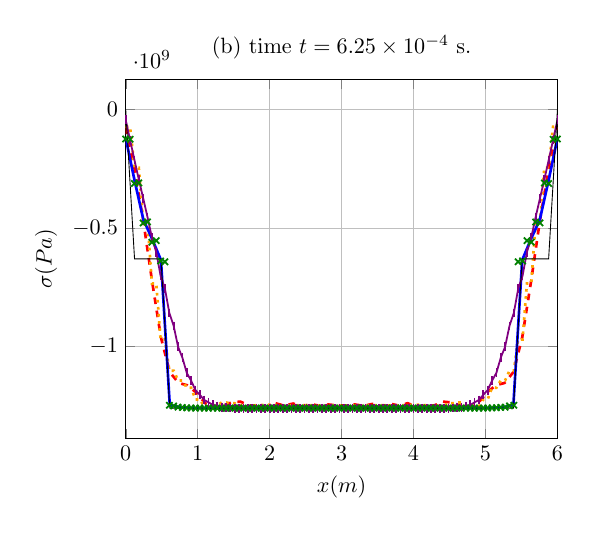
\begin{tikzpicture}[scale=0.8]
\begin{axis}[xlabel=$x (m)$,ylabel=$\sigma (Pa)$,ymajorgrids=true,xmajorgrids=true,legend pos=outer north east,title={(b) time $t = 6.25\times 10^{-4} $ s.},xmin=0.,xmax=6.]
\addplot[Red,very thick,mark=none,dashed] coordinates {(0.0,-74686690.65430246) (0.12244897959183673,-248860978.1693335) (0.24489795918367346,-471505677.3136862) (0.36734693877551017,-727347550.4714894) (0.4897959183673469,-963308331.6520433) (0.6122448979591837,-1108824904.6085515) (0.7346938775510203,-1154837713.915547) (0.8571428571428571,-1164658358.6882505) (0.9795918367346939,-1195327833.6731591) (1.1020408163265305,-1239722495.17177) (1.2244897959183674,-1262625036.5763078) (1.346938775510204,-1250850727.3360605) (1.4693877551020407,-1237335621.1098552) (1.5918367346938775,-1233570784.670482) (1.7142857142857142,-1250022356.590519) (1.836734693877551,-1250064510.2383804) (1.9591836734693877,-1255304260.9119728) (2.0816326530612246,-1240464014.9742188) (2.204081632653061,-1250749408.0219655) (2.326530612244898,-1241771881.0316234) (2.4489795918367347,-1254655253.5739675) (2.571428571428571,-1243386642.1602688) (2.693877551020408,-1251564997.8232079) (2.816326530612245,-1245650942.428049) (2.9387755102040813,-1249901934.3884947) (3.061224489795918,-1249901934.3884926) (3.183673469387755,-1245650942.4280505) (3.306122448979592,-1251564997.8232062) (3.4285714285714284,-1243386642.160271) (3.5510204081632653,-1254655253.5739667) (3.673469387755102,-1241771881.0316243) (3.7959183673469385,-1250749408.0219643) (3.9183673469387754,-1240464014.9742193) (4.040816326530612,-1255304260.911973) (4.163265306122449,-1250064510.238382) (4.285714285714286,-1250022356.59052) (4.408163265306122,-1233570784.670483) (4.530612244897959,-1237335621.1098552) (4.653061224489796,-1250850727.3360612) (4.775510204081632,-1262625036.5763083) (4.8979591836734695,-1239722495.1717708) (5.020408163265306,-1195327833.6731594) (5.142857142857142,-1164658358.688251) (5.26530612244898,-1154837713.915547) (5.387755102040816,-1108824904.6085508) (5.5102040816326525,-963308331.652042) (5.63265306122449,-727347550.4714878) (5.755102040816326,-471505677.3136848) (5.877551020408163,-248860978.16933236) (6.0,-74686690.65430167) };
\addplot[Orange,very thick,mark=none,dotted] coordinates {(0.0,-72186593.07108305) (0.06060606060606061,-72186593.07108305) (0.12121212121212122,-245686493.40496877) (0.18181818181818182,-245686493.40496877) (0.24242424242424243,-474670673.0513873) (0.30303030303030304,-474670673.0513873) (0.36363636363636365,-734906817.2671752) (0.42424242424242425,-734906817.2671752) (0.48484848484848486,-970962001.9023491) (0.5454545454545454,-970962001.9023491) (0.6060606060606061,-1103271474.8574238) (0.6666666666666667,-1103271474.8574238) (0.7272727272727273,-1144170322.1258416) (0.7878787878787878,-1144170322.1258416) (0.8484848484848485,-1175098111.1407657) (0.9090909090909092,-1175098111.1407657) (0.9696969696969697,-1224410658.5301867) (1.0303030303030303,-1224410658.5301867) (1.0909090909090908,-1254385387.017002) (1.1515151515151516,-1254385387.017002) (1.2121212121212122,-1249105579.9476206) (1.2727272727272727,-1249105579.9476206) (1.3333333333333335,-1237157219.1940255) (1.393939393939394,-1237157219.1940255) (1.4545454545454546,-1240480450.514414) (1.5151515151515151,-1240480450.514414) (1.5757575757575757,-1250188640.1270242) (1.6363636363636365,-1250188640.1270242) (1.696969696969697,-1252250954.763) (1.7575757575757576,-1252250954.763) (1.8181818181818183,-1248402726.9188023) (1.878787878787879,-1248402726.9188023) (1.9393939393939394,-1246829218.0208151) (2.0,-1246829218.0208151) (2.0606060606060606,-1248579916.6035461) (2.121212121212121,-1248579916.6035461) (2.1818181818181817,-1249829973.3539176) (2.2424242424242427,-1249829973.3539176) (2.303030303030303,-1249407075.968172) (2.3636363636363638,-1249407075.968172) (2.4242424242424243,-1248930440.9460857) (2.484848484848485,-1248930440.9460857) (2.5454545454545454,-1249182413.9939532) (2.606060606060606,-1249182413.9939532) (2.666666666666667,-1249584324.22758) (2.7272727272727275,-1249584324.22758) (2.787878787878788,-1249734146.6328998) (2.8484848484848486,-1249734146.6328998) (2.909090909090909,-1249747490.5668778) (2.9696969696969697,-1249747490.5668778) (3.0303030303030303,-1249747490.5668783) (3.090909090909091,-1249747490.5668783) (3.1515151515151514,-1249734146.6329007) (3.2121212121212124,-1249734146.6329007) (3.272727272727273,-1249584324.2275805) (3.3333333333333335,-1249584324.2275805) (3.393939393939394,-1249182413.993953) (3.4545454545454546,-1249182413.993953) (3.515151515151515,-1248930440.946085) (3.5757575757575757,-1248930440.946085) (3.6363636363636367,-1249407075.9681716) (3.6969696969696972,-1249407075.9681716) (3.757575757575758,-1249829973.3539178) (3.8181818181818183,-1249829973.3539178) (3.878787878787879,-1248579916.6035466) (3.9393939393939394,-1248579916.6035466) (4.0,-1246829218.0208151) (4.0606060606060606,-1246829218.0208151) (4.121212121212121,-1248402726.9188023) (4.181818181818182,-1248402726.9188023) (4.242424242424242,-1252250954.7630002) (4.303030303030303,-1252250954.7630002) (4.363636363636363,-1250188640.1270244) (4.424242424242425,-1250188640.1270244) (4.484848484848485,-1240480450.5144138) (4.545454545454546,-1240480450.5144138) (4.606060606060606,-1237157219.194025) (4.666666666666667,-1237157219.194025) (4.7272727272727275,-1249105579.9476204) (4.787878787878788,-1249105579.9476204) (4.848484848484849,-1254385387.0170026) (4.909090909090909,-1254385387.0170026) (4.96969696969697,-1224410658.5301871) (5.03030303030303,-1224410658.5301871) (5.090909090909091,-1175098111.140766) (5.151515151515151,-1175098111.140766) (5.212121212121212,-1144170322.125842) (5.2727272727272725,-1144170322.125842) (5.333333333333334,-1103271474.8574243) (5.3939393939393945,-1103271474.8574243) (5.454545454545455,-970962001.902349) (5.515151515151516,-970962001.902349) (5.575757575757576,-734906817.2671752) (5.636363636363637,-734906817.2671752) (5.696969696969697,-474670673.05138755) (5.757575757575758,-474670673.05138755) (5.818181818181818,-245686493.40496898) (5.878787878787879,-245686493.40496898) (5.9393939393939394,-72186593.0710832) (6.0,-72186593.0710832) };
\addplot[Blue,very thick,mark=none,solid] coordinates {(0.0,-120597397.19248778) (0.12244897959183673,-298539345.15508544) (0.24489795918367346,-464504460.170754) (0.36734693877551017,-546627376.3559334) (0.4897959183673469,-635546108.2543886) (0.6122448979591837,-1247334335.3333962) (0.7346938775510203,-1255980074.5990539) (0.8571428571428571,-1259371705.5275755) (0.9795918367346939,-1260535220.1287405) (1.1020408163265305,-1260885267.5005968) (1.2244897959183674,-1260977777.705495) (1.346938775510204,-1260999265.6570995) (1.4693877551020407,-1261003650.0375175) (1.5918367346938775,-1261004434.5740557) (1.7142857142857142,-1261004557.3391547) (1.836734693877551,-1261004574.0682204) (1.9591836734693877,-1261004576.0419452) (2.0816326530612246,-1261004576.241996) (2.204081632653061,-1261004576.2592359) (2.326530612244898,-1261004576.260481) (2.4489795918367347,-1261004576.260556) (2.571428571428571,-1261004576.2605588) (2.693877551020408,-1261004576.260559) (2.816326530612245,-1261004576.2605588) (2.9387755102040813,-1261004576.260559) (3.061224489795918,-1261004576.2605584) (3.183673469387755,-1261004576.2605586) (3.306122448979592,-1261004576.2605588) (3.4285714285714284,-1261004576.2605581) (3.5510204081632653,-1261004576.2605555) (3.673469387755102,-1261004576.260481) (3.7959183673469385,-1261004576.2592354) (3.9183673469387754,-1261004576.2419953) (4.040816326530612,-1261004576.0419443) (4.163265306122449,-1261004574.06822) (4.285714285714286,-1261004557.3391542) (4.408163265306122,-1261004434.5740552) (4.530612244897959,-1261003650.037517) (4.653061224489796,-1260999265.6570988) (4.775510204081632,-1260977777.7054946) (4.8979591836734695,-1260885267.500596) (5.020408163265306,-1260535220.1287398) (5.142857142857142,-1259371705.5275738) (5.26530612244898,-1255980074.5990536) (5.387755102040816,-1247334335.3333952) (5.5102040816326525,-635546108.2543867) (5.63265306122449,-546627376.3559326) (5.755102040816326,-464504460.1707534) (5.877551020408163,-298539345.15508515) (6.0,-120597397.19248791) };
\addplot[Purple,thick,mark=|,solid] coordinates {(0.0,-43439158.01953824) (0.06060606060606061,-128494718.82956168) (0.12121212121212122,-212712806.4484778) (0.18181818181818182,-294968746.093467) (0.24242424242424243,-374066686.2634123) (0.30303030303030304,-454380990.25937665) (0.36363636363636365,-540156903.2805651) (0.42424242424242425,-602480956.5032418) (0.48484848484848486,-702661585.1512607) (0.5454545454545454,-756997379.9274446) (0.6060606060606061,-859011324.2404706) (0.6666666666666667,-914140387.8341031) (0.7272727272727273,-1001733202.5250769) (0.7878787878787878,-1048303078.4017226) (0.8484848484848485,-1112416155.8061078) (0.9090909090909092,-1145155832.8175488) (0.9696969696969697,-1185261988.985457) (1.0303030303030303,-1204786235.0815058) (1.0909090909090908,-1226655831.3690634) (1.1515151515151516,-1236845694.8683596) (1.2121212121212122,-1247415339.0967982) (1.2727272727272727,-1252155381.0243487) (1.3333333333333335,-1256710201.5466359) (1.393939393939394,-1258689335.4211235) (1.4545454545454546,-1260456486.190056) (1.5151515151515151,-1261197436.235882) (1.5757575757575757,-1261810365.4044876) (1.6363636363636365,-1262048555.9214687) (1.696969696969697,-1262232771.7377496) (1.7575757575757576,-1262267932.0178628) (1.8181818181818183,-1262317140.869429) (1.878787878787879,-1262273539.5537865) (1.9393939393939394,-1262278489.6867273) (2.0,-1262229915.5005774) (2.0606060606060606,-1262220408.763863) (2.121212121212121,-1262174209.4696336) (2.1818181818181817,-1262179981.2050242) (2.2424242424242427,-1262122756.5305994) (2.303030303030303,-1262166768.744628) (2.3636363636363638,-1262087669.6055806) (2.4242424242424243,-1262155242.0676785) (2.484848484848485,-1262097413.4000623) (2.5454545454545454,-1262171888.997602) (2.606060606060606,-1262117114.7579942) (2.666666666666667,-1262226451.4058053) (2.7272727272727275,-1262121200.847136) (2.787878787878788,-1262339443.020975) (2.8484848484848486,-1262066956.6541011) (2.909090909090909,-1262521430.1991065) (2.9696969696969697,-1261921359.640449) (3.0303030303030303,-1261921359.6404493) (3.090909090909091,-1262521430.1991067) (3.1515151515151514,-1262066956.6541014) (3.2121212121212124,-1262339443.0209754) (3.272727272727273,-1262121200.8471358) (3.3333333333333335,-1262226451.405806) (3.393939393939394,-1262117114.7579951) (3.4545454545454546,-1262171888.9976025) (3.515151515151515,-1262097413.4000628) (3.5757575757575757,-1262155242.0676794) (3.6363636363636367,-1262087669.6055813) (3.6969696969696972,-1262166768.744628) (3.757575757575758,-1262122756.5305994) (3.8181818181818183,-1262179981.2050242) (3.878787878787879,-1262174209.4696333) (3.9393939393939394,-1262220408.7638628) (4.0,-1262229915.5005774) (4.0606060606060606,-1262278489.6867273) (4.121212121212121,-1262273539.5537865) (4.181818181818182,-1262317140.8694305) (4.242424242424242,-1262267932.0178633) (4.303030303030303,-1262232771.7377505) (4.363636363636363,-1262048555.9214697) (4.424242424242425,-1261810365.4044883) (4.484848484848485,-1261197436.2358823) (4.545454545454546,-1260456486.1900568) (4.606060606060606,-1258689335.4211237) (4.666666666666667,-1256710201.5466368) (4.7272727272727275,-1252155381.0243497) (4.787878787878788,-1247415339.096799) (4.848484848484849,-1236845694.8683605) (4.909090909090909,-1226655831.3690639) (4.96969696969697,-1204786235.0815067) (5.03030303030303,-1185261988.9854574) (5.090909090909091,-1145155832.8175497) (5.151515151515151,-1112416155.8061085) (5.212121212121212,-1048303078.4017233) (5.2727272727272725,-1001733202.5250776) (5.333333333333334,-914140387.834104) (5.3939393939393945,-859011324.2404717) (5.454545454545455,-756997379.9274455) (5.515151515151516,-702661585.1512614) (5.575757575757576,-602480956.5032421) (5.636363636363637,-540156903.2805656) (5.696969696969697,-454380990.25937706) (5.757575757575758,-374066686.26341283) (5.818181818181818,-294968746.09346735) (5.878787878787879,-212712806.44847828) (5.9393939393939394,-128494718.82956178) (6.0,-43439158.019538306) };
\addplot[Green,thick,mark=x,only marks] coordinates {(0.0,-124149916.18460932) (0.06060606060606061,-125384025.95198976) (0.12121212121212122,-312191395.454492) (0.18181818181818182,-309823612.32028496) (0.24242424242424243,-478839586.50914454) (0.30303030303030304,-474422726.8389135) (0.36363636363636365,-560023095.785606) (0.42424242424242425,-553441168.2048206) (0.48484848484848486,-639348195.1618631) (0.5454545454545454,-642840843.3429394) (0.6060606060606061,-1249244226.3218632) (0.6666666666666667,-1251996686.3855102) (0.7272727272727273,-1257129205.37515) (0.7878787878787878,-1258189385.686948) (0.8484848484848485,-1259909142.5036347) (0.9090909090909092,-1260253063.700632) (0.9696969696969697,-1260739786.195639) (1.0303030303030303,-1260833818.3494694) (1.0909090909090908,-1260950011.0851812) (1.1515151515151516,-1260971641.1801379) (1.2121212121212122,-1260995018.2511435) (1.2727272727272727,-1260999205.0818741) (1.3333333333333335,-1261003073.8839324) (1.393939393939394,-1261003729.7383952) (1.4545454545454546,-1261004222.6859503) (1.5151515151515151,-1261004299.406877) (1.5757575757575757,-1261004499.1892421) (1.6363636363636365,-1261004544.8157115) (1.696969696969697,-1261004335.4465394) (1.7575757575757576,-1261004315.5457916) (1.8181818181818183,-1261004554.3249235) (1.878787878787879,-1261004539.201182) (1.9393939393939394,-1261004509.2896533) (2.0,-1261004479.0183125) (2.0606060606060606,-1261004581.0248919) (2.121212121212121,-1261004530.8669846) (2.1818181818181817,-1261004594.5349371) (2.2424242424242427,-1261004535.9740446) (2.303030303030303,-1261004688.980403) (2.3636363636363638,-1261004531.5634973) (2.4242424242424243,-1261004753.5964737) (2.484848484848485,-1261004491.241939) (2.5454545454545454,-1261004855.8046663) (2.606060606060606,-1261004170.2011797) (2.666666666666667,-1261005415.5085306) (2.7272727272727275,-1261003664.942618) (2.787878787878788,-1261005905.0268464) (2.8484848484848486,-1261003146.0581243) (2.909090909090909,-1261018444.8195553) (2.9696969696969697,-1260990588.6825547) (3.0303030303030303,-1260990588.6825557) (3.090909090909091,-1261018444.8195562) (3.1515151515151514,-1261003146.0581238) (3.2121212121212124,-1261005905.0268452) (3.272727272727273,-1261003664.9426184) (3.3333333333333335,-1261005415.5085318) (3.393939393939394,-1261004170.2011807) (3.4545454545454546,-1261004855.804668) (3.515151515151515,-1261004491.241938) (3.5757575757575757,-1261004753.5964735) (3.6363636363636367,-1261004531.563497) (3.6969696969696972,-1261004688.9804025) (3.757575757575758,-1261004535.9740455) (3.8181818181818183,-1261004594.5349386) (3.878787878787879,-1261004530.8669853) (3.9393939393939394,-1261004581.0248923) (4.0,-1261004479.0183132) (4.0606060606060606,-1261004509.2896538) (4.121212121212121,-1261004539.201182) (4.181818181818182,-1261004554.3249235) (4.242424242424242,-1261004315.5457911) (4.303030303030303,-1261004335.4465387) (4.363636363636363,-1261004544.815712) (4.424242424242425,-1261004499.1892428) (4.484848484848485,-1261004299.4068773) (4.545454545454546,-1261004222.6859503) (4.606060606060606,-1261003729.7383952) (4.666666666666667,-1261003073.8839328) (4.7272727272727275,-1260999205.0818748) (4.787878787878788,-1260995018.2511437) (4.848484848484849,-1260971641.1801379) (4.909090909090909,-1260950011.0851815) (4.96969696969697,-1260833818.3494704) (5.03030303030303,-1260739786.1956398) (5.090909090909091,-1260253063.7006326) (5.151515151515151,-1259909142.5036354) (5.212121212121212,-1258189385.6869476) (5.2727272727272725,-1257129205.3751497) (5.333333333333334,-1251996686.3855097) (5.3939393939393945,-1249244226.3218625) (5.454545454545455,-642840843.3429406) (5.515151515151516,-639348195.1618624) (5.575757575757576,-553441168.2048205) (5.636363636363637,-560023095.7856064) (5.696969696969697,-474422726.8389133) (5.757575757575758,-478839586.50914484) (5.818181818181818,-309823612.320285) (5.878787878787879,-312191395.4544924) (5.9393939393939394,-125384025.95198983) (6.0,-124149916.18460946) };
\addplot[black,thin,mark=none,solid] coordinates {(0.0,-0.0) (0.12244897959183673,-630502288.1302795) (0.24489795918367346,-630502288.1302795) (0.36734693877551017,-630502288.1302795) (0.4897959183673469,-630502288.1302795) (0.6122448979591837,-1261004576.260559) (0.7346938775510203,-1261004576.260559) (0.8571428571428571,-1261004576.260559) (0.9795918367346939,-1261004576.260559) (1.1020408163265305,-1261004576.260559) (1.2244897959183674,-1261004576.260559) (1.346938775510204,-1261004576.260559) (1.4693877551020407,-1261004576.260559) (1.5918367346938775,-1261004576.260559) (1.7142857142857142,-1261004576.260559) (1.836734693877551,-1261004576.260559) (1.9591836734693877,-1261004576.260559) (2.0816326530612246,-1261004576.260559) (2.204081632653061,-1261004576.260559) (2.326530612244898,-1261004576.260559) (2.4489795918367347,-1261004576.260559) (2.571428571428571,-1261004576.260559) (2.693877551020408,-1261004576.260559) (2.816326530612245,-1261004576.260559) (2.9387755102040813,-1261004576.260559) (3.061224489795918,-1261004576.260559) (3.183673469387755,-1261004576.260559) (3.306122448979592,-1261004576.260559) (3.4285714285714284,-1261004576.260559) (3.5510204081632653,-1261004576.260559) (3.673469387755102,-1261004576.260559) (3.7959183673469385,-1261004576.260559) (3.9183673469387754,-1261004576.260559) (4.040816326530612,-1261004576.260559) (4.163265306122449,-1261004576.260559) (4.285714285714286,-1261004576.260559) (4.408163265306122,-1261004576.260559) (4.530612244897959,-1261004576.260559) (4.653061224489796,-1261004576.260559) (4.775510204081632,-1261004576.260559) (4.8979591836734695,-1261004576.260559) (5.020408163265306,-1261004576.260559) (5.142857142857142,-1261004576.260559) (5.26530612244898,-1261004576.260559) (5.387755102040816,-1261004576.260559) (5.5102040816326525,-630502288.1302795) (5.63265306122449,-630502288.1302795) (5.755102040816326,-630502288.1302795) (5.877551020408163,-630502288.1302795) (6.0,-0.0) };
%\legend{usl 1ppc,usl 2ppc,dgmpm 1ppc,dgmpm 2ppc,dgmpm 2ppc (RK2),exact}
\end{axis}
\end{tikzpicture}
%%% Local Variables:
%%% mode: latex
%%% TeX-master: "../../mainManuscript"
%%% End:
}
  {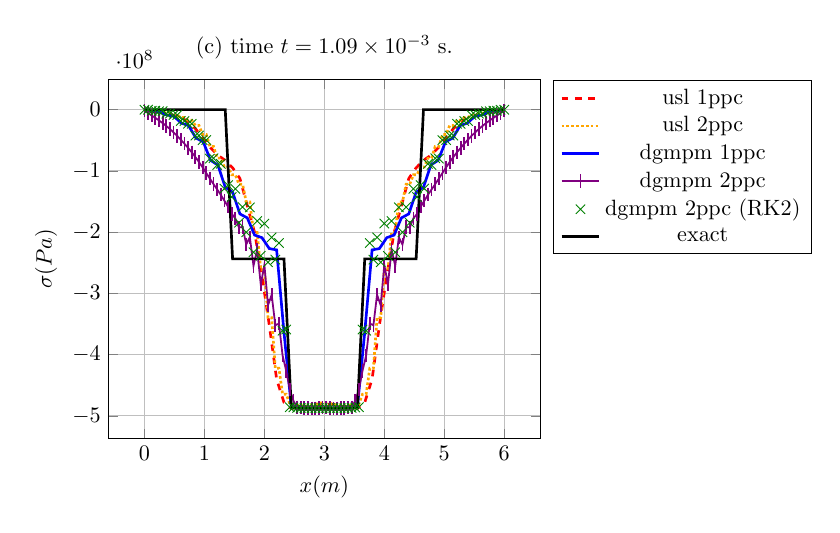
\begin{tikzpicture}[scale=0.8]
\begin{axis}[xlabel=$x (m)$,ylabel=$\sigma (Pa)$,ymajorgrids=true,xmajorgrids=true,legend pos=outer north east,title={(c) time $t = 1.09\times 10^{-3} $ s.}]
\addplot[Red,very thick,mark=none,dashed,mark size=3pt] coordinates {(0.0,-679166.0601331755) (0.12244897959183673,-2368189.594188208) (0.24489795918367346,-4606456.556212341) (0.36734693877551017,-6961578.395676694) (0.4897959183673469,-9332760.287028607) (0.6122448979591837,-12938682.464591796) (0.7346938775510203,-20102821.471402142) (0.8571428571428571,-32015823.341737133) (0.9795918367346939,-47676454.15860757) (1.1020408163265305,-62502940.42234602) (1.2244897959183674,-74544680.06037714) (1.346938775510204,-82775603.38522142) (1.4693877551020407,-94947363.4179823) (1.5918367346938775,-112415785.44002911) (1.7142857142857142,-156774491.63523546) (1.836734693877551,-200654618.50473383) (1.9591836734693877,-270646588.3413816) (2.0816326530612246,-351928629.9311485) (2.204081632653061,-440064160.15512294) (2.326530612244898,-477934424.91056436) (2.4489795918367347,-487815276.0764712) (2.571428571428571,-485351241.33413374) (2.693877551020408,-484406188.97201383) (2.816326530612245,-481035531.7602433) (2.9387755102040813,-481038509.8228564) (3.061224489795918,-481038509.8228558) (3.183673469387755,-481035531.7602443) (3.306122448979592,-484406188.9720135) (3.4285714285714284,-485351241.3341341) (3.5510204081632653,-487815276.07647014) (3.673469387755102,-477934424.9105651) (3.7959183673469385,-440064160.15512156) (3.9183673469387754,-351928629.931148) (4.040816326530612,-270646588.34138024) (4.163265306122449,-200654618.50473374) (4.285714285714286,-156774491.63523474) (4.408163265306122,-112415785.44002907) (4.530612244897959,-94947363.41798277) (4.653061224489796,-82775603.38522187) (4.775510204081632,-74544680.06037733) (4.8979591836734695,-62502940.42234604) (5.020408163265306,-47676454.158607304) (5.142857142857142,-32015823.341736842) (5.26530612244898,-20102821.471402) (5.387755102040816,-12938682.46459166) (5.5102040816326525,-9332760.287028512) (5.63265306122449,-6961578.395676572) (5.755102040816326,-4606456.55621225) (5.877551020408163,-2368189.594188123) (6.0,-679166.0601331636) };
\addplot[Orange,very thick,mark=none,densely dotted,mark size=3pt] coordinates {(0.0,-512829.37356199906) (0.06060606060606061,-512829.37356199906) (0.12121212121212122,-1685977.6907792736) (0.18181818181818182,-1685977.6907792736) (0.24242424242424243,-3409631.957049818) (0.30303030303030304,-3409631.957049818) (0.36363636363636365,-5994518.467970753) (0.42424242424242425,-5994518.467970753) (0.48484848484848486,-9186608.055434104) (0.5454545454545454,-9186608.055434104) (0.6060606060606061,-12632033.888351096) (0.6666666666666667,-12632033.888351096) (0.7272727272727273,-17308370.109125804) (0.7878787878787878,-17308370.109125804) (0.8484848484848485,-25927147.931033082) (0.9090909090909092,-25927147.931033082) (0.9696969696969697,-40719694.7337496) (1.0303030303030303,-40719694.7337496) (1.0909090909090908,-60222421.752752535) (1.1515151515151516,-60222421.752752535) (1.2121212121212122,-79232798.7243564) (1.2727272727272727,-79232798.7243564) (1.3333333333333335,-93917910.36545579) (1.393939393939394,-93917910.36545579) (1.4545454545454546,-106296964.05562654) (1.5151515151515151,-106296964.05562654) (1.5757575757575757,-121857025.50296684) (1.6363636363636365,-121857025.50296684) (1.696969696969697,-150591571.19633642) (1.7575757575757576,-150591571.19633642) (1.8181818181818183,-200655220.68880683) (1.878787878787879,-200655220.68880683) (1.9393939393939394,-261493503.50548327) (2.0,-261493503.50548327) (2.0606060606060606,-339524928.63039523) (2.121212121212121,-339524928.63039523) (2.1818181818181817,-422131801.353524) (2.2424242424242427,-422131801.353524) (2.303030303030303,-464494091.2915379) (2.3636363636363638,-464494091.2915379) (2.4242424242424243,-480288801.84594995) (2.484848484848485,-480288801.84594995) (2.5454545454545454,-482971319.0696361) (2.606060606060606,-482971319.0696361) (2.666666666666667,-484006263.5397973) (2.7272727272727275,-484006263.5397973) (2.787878787878788,-481823971.2401126) (2.8484848484848486,-481823971.2401126) (2.909090909090909,-478820708.8588188) (2.9696969696969697,-478820708.8588188) (3.0303030303030303,-478820708.8588188) (3.090909090909091,-478820708.8588188) (3.1515151515151514,-481823971.24011296) (3.2121212121212124,-481823971.24011296) (3.272727272727273,-484006263.53979766) (3.3333333333333335,-484006263.53979766) (3.393939393939394,-482971319.0696361) (3.4545454545454546,-482971319.0696361) (3.515151515151515,-480288801.84594995) (3.5757575757575757,-480288801.84594995) (3.6363636363636367,-464494091.2915379) (3.6969696969696972,-464494091.2915379) (3.757575757575758,-422131801.3535244) (3.8181818181818183,-422131801.3535244) (3.878787878787879,-339524928.6303949) (3.9393939393939394,-339524928.6303949) (4.0,-261493503.50548312) (4.0606060606060606,-261493503.50548312) (4.121212121212121,-200655220.68880683) (4.181818181818182,-200655220.68880683) (4.242424242424242,-150591571.1963363) (4.303030303030303,-150591571.1963363) (4.363636363636363,-121857025.50296697) (4.424242424242425,-121857025.50296697) (4.484848484848485,-106296964.05562642) (4.545454545454546,-106296964.05562642) (4.606060606060606,-93917910.36545563) (4.666666666666667,-93917910.36545563) (4.7272727272727275,-79232798.7243563) (4.787878787878788,-79232798.7243563) (4.848484848484849,-60222421.752752505) (4.909090909090909,-60222421.752752505) (4.96969696969697,-40719694.73374956) (5.03030303030303,-40719694.73374956) (5.090909090909091,-25927147.93103303) (5.151515151515151,-25927147.93103303) (5.212121212121212,-17308370.109125733) (5.2727272727272725,-17308370.109125733) (5.333333333333334,-12632033.888351053) (5.3939393939393945,-12632033.888351053) (5.454545454545455,-9186608.05543412) (5.515151515151516,-9186608.05543412) (5.575757575757576,-5994518.467970843) (5.636363636363637,-5994518.467970843) (5.696969696969697,-3409631.957049952) (5.757575757575758,-3409631.957049952) (5.818181818181818,-1685977.690779395) (5.878787878787879,-1685977.690779395) (5.9393939393939394,-512829.37356205017) (6.0,-512829.37356205017) };
\addplot[Blue,very thick,mark=none,solid,mark size=3pt] coordinates {(0.0,-298852.1952411225) (0.12244897959183673,-2592980.4740912793) (0.24489795918367346,-3560236.4322381816) (0.36734693877551017,-8652722.221047912) (0.4897959183673469,-10777216.673686886) (0.6122448979591837,-21974314.707157355) (0.7346938775510203,-26009924.918005344) (0.8571428571428571,-46347563.10657899) (0.9795918367346939,-52593345.171819046) (1.1020408163265305,-82683979.65035231) (1.2244897959183674,-90525380.97285904) (1.346938775510204,-126773557.44849168) (1.4693877551020407,-134743667.28836828) (1.5918367346938775,-170219249.4978279) (1.7142857142857142,-176744937.7749974) (1.836734693877551,-204799464.24688196) (1.9591836734693877,-209064122.25232974) (2.0816326530612246,-226820170.49378502) (2.204081632653061,-229011964.3130221) (2.326530612244898,-363270795.9137317) (2.4489795918367347,-485529213.90073514) (2.571428571428571,-486748760.1951447) (2.693877551020408,-487164866.56783277) (2.816326530612245,-487268871.16624963) (2.9387755102040813,-487285807.7274521) (3.061224489795918,-487285807.7274521) (3.183673469387755,-487268871.16624963) (3.306122448979592,-487164866.56783277) (3.4285714285714284,-486748760.1951447) (3.5510204081632653,-485529213.90073514) (3.673469387755102,-363270795.91372997) (3.7959183673469385,-229011964.3130223) (3.9183673469387754,-226820170.49378502) (4.040816326530612,-209064122.25232938) (4.163265306122449,-204799464.2468816) (4.285714285714286,-176744937.77499697) (4.408163265306122,-170219249.4978276) (4.530612244897959,-134743667.28836808) (4.653061224489796,-126773557.44849148) (4.775510204081632,-90525380.9728589) (4.8979591836734695,-82683979.65035222) (5.020408163265306,-52593345.171819076) (5.142857142857142,-46347563.10657902) (5.26530612244898,-26009924.918005634) (5.387755102040816,-21974314.707157686) (5.5102040816326525,-10777216.673687106) (5.63265306122449,-8652722.22104813) (5.755102040816326,-3560236.4322383474) (5.877551020408163,-2592980.4740913147) (6.0,-298852.1952412414) };
\addplot[Purple,thick,mark=|,solid,mark size=3pt] coordinates {(0.0,-1967506.1700863338) (0.06060606060606061,-5640032.662143143) (0.12121212121212122,-9656978.414919749) (0.18181818181818182,-13511820.529648876) (0.24242424242424243,-17791285.14768848) (0.30303030303030304,-22020954.760085706) (0.36363636363636365,-26810841.63481511) (0.42424242424242425,-31669769.847401485) (0.48484848484848486,-37219038.25874583) (0.5454545454545454,-42898302.86376866) (0.6060606060606061,-49215331.978578255) (0.6666666666666667,-55631508.92977342) (0.7272727272727273,-62575105.835719146) (0.7878787878787878,-69650368.30460997) (0.8484848484848485,-77440912.11382866) (0.9090909090909092,-85513317.74757525) (0.9696969696969697,-94394406.18118168) (1.0303030303030303,-103458727.33292748) (1.0909090909090908,-112622821.36245859) (1.1515151515151516,-121624138.89888178) (1.2121212121212122,-130341670.55898608) (1.2727272727272727,-139154542.84528217) (1.3333333333333335,-148830679.63128546) (1.393939393939394,-158542307.8017911) (1.4545454545454546,-170175255.01202118) (1.5151515151515151,-177512130.9706464) (1.5757575757575757,-192468554.83417034) (1.6363636363636365,-191410973.67950493) (1.696969696969697,-220188643.16229337) (1.7575757575757576,-208348179.3812332) (1.8181818181818183,-255105244.69638902) (1.878787878787879,-228761423.37895402) (1.9393939393939394,-285472179.8898197) (2.0,-253525121.96460363) (2.0606060606060606,-319389070.9725514) (2.121212121212121,-302097367.51271814) (2.1818181818181817,-351940004.91030246) (2.2424242424242427,-349259097.20874596) (2.303030303030303,-401088439.8898511) (2.3636363636363638,-426445036.100153) (2.4242424242424243,-456776041.9007156) (2.484848484848485,-475327504.30100346) (2.5454545454545454,-485932720.49084026) (2.606060606060606,-486800863.6836889) (2.666666666666667,-487206914.08181626) (2.7272727272727275,-487221866.2556566) (2.787878787878788,-487293102.56783485) (2.8484848484848486,-487291983.48275816) (2.909090909090909,-486820130.2994909) (2.9696969696969697,-486154460.1484115) (3.0303030303030303,-486154460.1484115) (3.090909090909091,-486820130.2994909) (3.1515151515151514,-487291983.4827589) (3.2121212121212124,-487293102.56783485) (3.272727272727273,-487221866.2556566) (3.3333333333333335,-487206914.08181626) (3.393939393939394,-486800863.68368924) (3.4545454545454546,-485932720.4908413) (3.515151515151515,-475327504.30100375) (3.5757575757575757,-456776041.90071523) (3.6363636363636367,-426445036.10015374) (3.6969696969696972,-401088439.8898514) (3.757575757575758,-349259097.2087466) (3.8181818181818183,-351940004.91030276) (3.878787878787879,-302097367.5127176) (3.9393939393939394,-319389070.9725512) (4.0,-253525121.96460345) (4.0606060606060606,-285472179.8898196) (4.121212121212121,-228761423.3789541) (4.181818181818182,-255105244.69638902) (4.242424242424242,-208348179.3812334) (4.303030303030303,-220188643.16229364) (4.363636363636363,-191410973.6795053) (4.424242424242425,-192468554.83417064) (4.484848484848485,-177512130.97064662) (4.545454545454546,-170175255.01202148) (4.606060606060606,-158542307.8017913) (4.666666666666667,-148830679.63128573) (4.7272727272727275,-139154542.84528223) (4.787878787878788,-130341670.55898641) (4.848484848484849,-121624138.89888197) (4.909090909090909,-112622821.36245887) (4.96969696969697,-103458727.33292772) (5.03030303030303,-94394406.18118192) (5.090909090909091,-85513317.74757543) (5.151515151515151,-77440912.11382888) (5.212121212121212,-69650368.30461016) (5.2727272727272725,-62575105.83571933) (5.333333333333334,-55631508.92977359) (5.3939393939393945,-49215331.97857844) (5.454545454545455,-42898302.863768816) (5.515151515151516,-37219038.25874599) (5.575757575757576,-31669769.847401626) (5.636363636363637,-26810841.634815253) (5.696969696969697,-22020954.760085825) (5.757575757575758,-17791285.147688594) (5.818181818181818,-13511820.529648978) (5.878787878787879,-9656978.414919829) (5.9393939393939394,-5640032.662143192) (6.0,-1967506.1700863515) };
\addplot[Green,thin,mark=x,only marks,mark size=3pt] coordinates {(0.0,-230769.40948159585) (0.06060606060606061,-230768.71951221325) (0.12121212121212122,-1765050.39034623) (0.18181818181818182,-1765048.7256776437) (0.24242424242424243,-2617614.5488237087) (0.30303030303030304,-2617595.5576229785) (0.36363636363636365,-6618855.725385412) (0.42424242424242425,-6618791.381126346) (0.48484848484848486,-8782768.896716146) (0.5454545454545454,-8782347.865813052) (0.6060606060606061,-18621957.945415) (0.6666666666666667,-18620353.83429409) (0.7272727272727273,-23151239.305377506) (0.7878787878787878,-23143055.39749537) (0.8484848484848485,-42429548.36143795) (0.9090909090909092,-42396573.934735104) (0.9696969696969697,-49952758.0967802) (1.0303030303030303,-49806565.98801953) (1.0909090909090908,-80012587.42975214) (1.1515151515151516,-79461376.35879174) (1.2121212121212122,-90415119.5727169) (1.2727272727272727,-88488293.78873543) (1.3333333333333335,-128889020.76572785) (1.393939393939394,-123386634.02232555) (1.4545454545454546,-142761259.00417286) (1.5151515151515151,-129449157.87721576) (1.5757575757575757,-184648477.15027985) (1.6363636363636365,-158996250.14018014) (1.696969696969697,-200285677.94521412) (1.7575757575757576,-159431830.86237475) (1.8181818181818183,-232788597.47549) (1.878787878787879,-181815073.16887435) (1.9393939393939394,-238716756.27113715) (2.0,-185991644.81247783) (2.0606060606060606,-249108768.01695433) (2.121212121212121,-208608151.93422446) (2.1818181818181817,-244796764.89630747) (2.2424242424242427,-217807407.36442074) (2.303030303030303,-360926830.0819958) (2.3636363636363638,-358951385.7834185) (2.4242424242424243,-485803376.4944678) (2.484848484848485,-486055584.43364054) (2.5454545454545454,-486867155.31944156) (2.606060606060606,-486947986.92719907) (2.666666666666667,-487200286.73057413) (2.7272727272727275,-487218951.17205155) (2.787878787878788,-487275506.6886281) (2.8484848484848486,-487278268.04119205) (2.909090909090909,-487286397.423194) (2.9696969696969697,-487286593.83864176) (3.0303030303030303,-487286593.83864176) (3.090909090909091,-487286397.423194) (3.1515151515151514,-487278268.04119205) (3.2121212121212124,-487275506.6886281) (3.272727272727273,-487218951.17205155) (3.3333333333333335,-487200286.73057413) (3.393939393939394,-486947986.92719907) (3.4545454545454546,-486867155.31944156) (3.515151515151515,-486055584.43364054) (3.5757575757575757,-485803376.4944678) (3.6363636363636367,-358951385.78341883) (3.6969696969696972,-360926830.08199614) (3.757575757575758,-217807407.3644211) (3.8181818181818183,-244796764.896308) (3.878787878787879,-208608151.93422586) (3.9393939393939394,-249108768.01695573) (4.0,-185991644.81247783) (4.0606060606060606,-238716756.27113697) (4.121212121212121,-181815073.16887408) (4.181818181818182,-232788597.47549027) (4.242424242424242,-159431830.86237472) (4.303030303030303,-200285677.9452144) (4.363636363636363,-158996250.1401801) (4.424242424242425,-184648477.15027985) (4.484848484848485,-129449157.87721583) (4.545454545454546,-142761259.0041731) (4.606060606060606,-123386634.02232562) (4.666666666666667,-128889020.76572803) (4.7272727272727275,-88488293.78873555) (4.787878787878788,-90415119.57271707) (4.848484848484849,-79461376.35879163) (4.909090909090909,-80012587.42975211) (4.96969696969697,-49806565.98801959) (5.03030303030303,-49952758.096780345) (5.090909090909091,-42396573.93473512) (5.151515151515151,-42429548.36143816) (5.212121212121212,-23143055.397495314) (5.2727272727272725,-23151239.305377506) (5.333333333333334,-18620353.834293906) (5.3939393939393945,-18621957.94541511) (5.454545454545455,-8782347.865813203) (5.515151515151516,-8782768.896716148) (5.575757575757576,-6618791.38112651) (5.636363636363637,-6618855.725385466) (5.696969696969697,-2617595.5576235284) (5.757575757575758,-2617614.5488236495) (5.818181818181818,-1765048.7256772814) (5.878787878787879,-1765050.390346396) (5.9393939393939394,-230768.71951233502) (6.0,-230769.4094818794) };
\addplot[black,very thick,mark=pentagone*,solid,mark size=3pt] coordinates {(0.0,-0.0) (0.12244897959183673,-0.0) (0.24489795918367346,-0.0) (0.36734693877551017,-0.0) (0.4897959183673469,-0.0) (0.6122448979591837,-0.0) (0.7346938775510203,-0.0) (0.8571428571428571,-0.0) (0.9795918367346939,-0.0) (1.1020408163265305,-0.0) (1.2244897959183674,-0.0) (1.346938775510204,-0.0) (1.4693877551020407,-243643578.04719847) (1.5918367346938775,-243643578.04719847) (1.7142857142857142,-243643578.04719847) (1.836734693877551,-243643578.04719847) (1.9591836734693877,-243643578.04719847) (2.0816326530612246,-243643578.04719847) (2.204081632653061,-243643578.04719847) (2.326530612244898,-243643578.04719847) (2.4489795918367347,-487287156.09439695) (2.571428571428571,-487287156.09439695) (2.693877551020408,-487287156.09439695) (2.816326530612245,-487287156.09439695) (2.9387755102040813,-487287156.09439695) (3.061224489795918,-487287156.09439695) (3.183673469387755,-487287156.09439695) (3.306122448979592,-487287156.09439695) (3.4285714285714284,-487287156.09439695) (3.5510204081632653,-487287156.09439695) (3.673469387755102,-243643578.04719847) (3.7959183673469385,-243643578.04719847) (3.9183673469387754,-243643578.04719847) (4.040816326530612,-243643578.04719847) (4.163265306122449,-243643578.04719847) (4.285714285714286,-243643578.04719847) (4.408163265306122,-243643578.04719847) (4.530612244897959,-243643578.04719847) (4.653061224489796,-0.0) (4.775510204081632,-0.0) (4.8979591836734695,-0.0) (5.020408163265306,-0.0) (5.142857142857142,-0.0) (5.26530612244898,-0.0) (5.387755102040816,-0.0) (5.5102040816326525,-0.0) (5.63265306122449,-0.0) (5.755102040816326,-0.0) (5.877551020408163,-0.0) (6.0,-0.0) };
\legend{usl 1ppc,usl 2ppc,dgmpm 1ppc,dgmpm 2ppc,dgmpm 2ppc (RK2),exact}
\end{axis}
\end{tikzpicture}
%%% Local Variables:
%%% mode: latex
%%% TeX-master: "../../mainManuscript"
%%% End:
}
  \caption{elastic-plastic RP stress}
  \label{fig:stress_elastoplastic_RP}
\end{figure}
\begin{figure}[h!]
  \centering
  {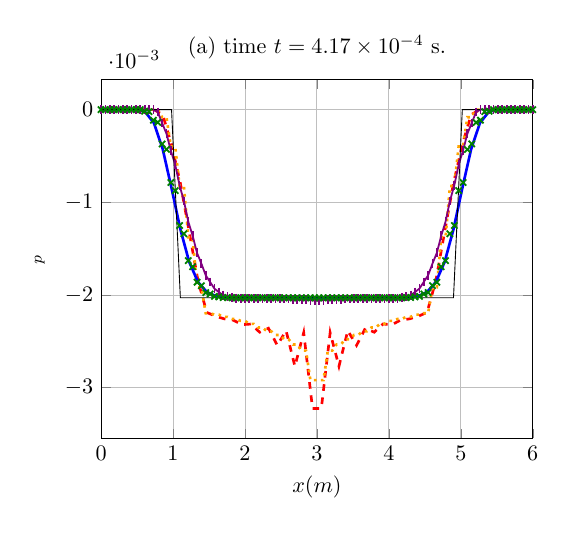
\begin{tikzpicture}[scale=0.8]
\begin{axis}[xlabel=$x (m)$,ylabel=$\eps^p$,ymajorgrids=true,xmajorgrids=true,legend pos=outer north east,title={(a) time $t = 4.17\times 10^{-4} $ s.},xmin=0.,xmax=6.]
\addplot[Red,very thick,mark=none,dashed] coordinates {(0.0,0.0) (0.12244897959183673,0.0) (0.24489795918367346,0.0) (0.36734693877551017,0.0) (0.4897959183673469,0.0) (0.6122448979591837,0.0) (0.7346938775510203,0.0) (0.8571428571428571,-5.5177825258810104e-05) (0.9795918367346939,-0.0003791196239632164) (1.1020408163265305,-0.0007942218458547296) (1.2244897959183674,-0.0013158519965027296) (1.346938775510204,-0.0018458090676901286) (1.4693877551020407,-0.002188794617508559) (1.5918367346938775,-0.002229697455331896) (1.7142857142857142,-0.002258121963594508) (1.836734693877551,-0.002271799079674154) (1.9591836734693877,-0.002320613632318322) (2.0816326530612246,-0.002313868472160546) (2.204081632653061,-0.0024020122032007017) (2.326530612244898,-0.0023588630990294623) (2.4489795918367347,-0.0025433455597807667) (2.571428571428571,-0.002385435935351422) (2.693877551020408,-0.0027693350417516906) (2.816326530612245,-0.0024065265204776445) (2.9387755102040813,-0.0032250612006492966) (3.061224489795918,-0.0032250612006492524) (3.183673469387755,-0.002406526520477666) (3.306122448979592,-0.0027693350417516823) (3.4285714285714284,-0.0023854359353514295) (3.5510204081632653,-0.0025433455597807628) (3.673469387755102,-0.002358863099029464) (3.7959183673469385,-0.0024020122032006983) (3.9183673469387754,-0.0023138684721605448) (4.040816326530612,-0.002320613632318319) (4.163265306122449,-0.0022717990796741546) (4.285714285714286,-0.0022581219635945077) (4.408163265306122,-0.0022296974553318956) (4.530612244897959,-0.0021887946175085595) (4.653061224489796,-0.001845809067690125) (4.775510204081632,-0.0013158519965027254) (4.8979591836734695,-0.0007942218458547295) (5.020408163265306,-0.0003791196239632123) (5.142857142857142,-5.5177825258808404e-05) (5.26530612244898,0.0) (5.387755102040816,0.0) (5.5102040816326525,0.0) (5.63265306122449,0.0) (5.755102040816326,0.0) (5.877551020408163,0.0) (6.0,0.0) };
\addplot[Orange,very thick,mark=none,dotted] coordinates {(0.0,0.0) (0.06060606060606061,0.0) (0.12121212121212122,0.0) (0.18181818181818182,0.0) (0.24242424242424243,0.0) (0.30303030303030304,0.0) (0.36363636363636365,0.0) (0.42424242424242425,0.0) (0.48484848484848486,0.0) (0.5454545454545454,0.0) (0.6060606060606061,0.0) (0.6666666666666667,0.0) (0.7272727272727273,0.0) (0.7878787878787878,0.0) (0.8484848484848485,-8.276994982638746e-05) (0.9090909090909092,-8.276994982638746e-05) (0.9696969696969697,-0.0003982743796454725) (1.0303030303030303,-0.0003982743796454725) (1.0909090909090908,-0.0008251664654092959) (1.1515151515151516,-0.0008251664654092959) (1.2121212121212122,-0.0013769280756316814) (1.2727272727272727,-0.0013769280756316814) (1.3333333333333335,-0.0019184552821342453) (1.393939393939394,-0.0019184552821342453) (1.4545454545454546,-0.0021968313010739355) (1.5151515151515151,-0.0021968313010739355) (1.5757575757575757,-0.0022123334205993417) (1.6363636363636365,-0.0022123334205993417) (1.696969696969697,-0.0022365941606657474) (1.7575757575757576,-0.0022365941606657474) (1.8181818181818183,-0.0022585940891309796) (1.878787878787879,-0.0022585940891309796) (1.9393939393939394,-0.0022798424574663194) (2.0,-0.0022798424574663194) (2.0606060606060606,-0.0023117041253564387) (2.121212121212121,-0.0023117041253564387) (2.1818181818181817,-0.002350782112768782) (2.2424242424242427,-0.002350782112768782) (2.303030303030303,-0.002390940396871615) (2.3636363636363638,-0.002390940396871615) (2.4242424242424243,-0.0024313395034050904) (2.484848484848485,-0.0024313395034050904) (2.5454545454545454,-0.002477563584428502) (2.606060606060606,-0.002477563584428502) (2.666666666666667,-0.0025344573000873694) (2.7272727272727275,-0.0025344573000873694) (2.787878787878788,-0.002600834768573611) (2.8484848484848486,-0.002600834768573611) (2.909090909090909,-0.0029191565184019295) (2.9696969696969697,-0.0029191565184019295) (3.0303030303030303,-0.0029191565184019273) (3.090909090909091,-0.0029191565184019273) (3.1515151515151514,-0.0026008347685736143) (3.2121212121212124,-0.0026008347685736143) (3.272727272727273,-0.002534457300087371) (3.3333333333333335,-0.002534457300087371) (3.393939393939394,-0.0024775635844285025) (3.4545454545454546,-0.0024775635844285025) (3.515151515151515,-0.0024313395034050896) (3.5757575757575757,-0.0024313395034050896) (3.6363636363636367,-0.002390940396871615) (3.6969696969696972,-0.002390940396871615) (3.757575757575758,-0.0023507821127687826) (3.8181818181818183,-0.0023507821127687826) (3.878787878787879,-0.002311704125356438) (3.9393939393939394,-0.002311704125356438) (4.0,-0.0022798424574663172) (4.0606060606060606,-0.0022798424574663172) (4.121212121212121,-0.00225859408913098) (4.181818181818182,-0.00225859408913098) (4.242424242424242,-0.002236594160665746) (4.303030303030303,-0.002236594160665746) (4.363636363636363,-0.0022123334205993426) (4.424242424242425,-0.0022123334205993426) (4.484848484848485,-0.002196831301073935) (4.545454545454546,-0.002196831301073935) (4.606060606060606,-0.0019184552821342445) (4.666666666666667,-0.0019184552821342445) (4.7272727272727275,-0.0013769280756316814) (4.787878787878788,-0.0013769280756316814) (4.848484848484849,-0.0008251664654092957) (4.909090909090909,-0.0008251664654092957) (4.96969696969697,-0.0003982743796454725) (5.03030303030303,-0.0003982743796454725) (5.090909090909091,-8.276994982638697e-05) (5.151515151515151,-8.276994982638697e-05) (5.212121212121212,0.0) (5.2727272727272725,0.0) (5.333333333333334,0.0) (5.3939393939393945,0.0) (5.454545454545455,0.0) (5.515151515151516,0.0) (5.575757575757576,0.0) (5.636363636363637,0.0) (5.696969696969697,0.0) (5.757575757575758,0.0) (5.818181818181818,0.0) (5.878787878787879,0.0) (5.9393939393939394,0.0) (6.0,0.0) };
\addplot[Blue,very thick,mark=none,solid] coordinates {(0.0,0.0) (0.12244897959183673,0.0) (0.24489795918367346,0.0) (0.36734693877551017,0.0) (0.4897959183673469,0.0) (0.6122448979591837,-2.4267855226065594e-05) (0.7346938775510203,-0.00014452073597361284) (0.8571428571428571,-0.0004275642401009131) (0.9795918367346939,-0.0008483282066457896) (1.1020408163265305,-0.0012913872123487611) (1.2244897959183674,-0.001642660920094959) (1.346938775510204,-0.0018602413103573651) (1.4693877551020407,-0.0019680574666657586) (1.5918367346938775,-0.00201146561977191) (1.7142857142857142,-0.002025805454394895) (1.836734693877551,-0.0020297136017104972) (1.9591836734693877,-0.002030593864489664) (2.0816326530612246,-0.002030757436013639) (2.204081632653061,-0.0020307823755532774) (2.326530612244898,-0.002030785465084119) (2.4489795918367347,-0.0020307857712710334) (2.571428571428571,-0.00203078579497771) (2.693877551020408,-0.0020307857963597366) (2.816326530612245,-0.002030785796416807) (2.9387755102040813,-0.002030785796418294) (3.061224489795918,-0.002030785796418294) (3.183673469387755,-0.0020307857964168056) (3.306122448979592,-0.002030785796359739) (3.4285714285714284,-0.0020307857949777124) (3.5510204081632653,-0.002030785771271032) (3.673469387755102,-0.002030785465084119) (3.7959183673469385,-0.002030782375553277) (3.9183673469387754,-0.0020307574360136386) (4.040816326530612,-0.002030593864489664) (4.163265306122449,-0.0020297136017104964) (4.285714285714286,-0.0020258054543948927) (4.408163265306122,-0.002011465619771909) (4.530612244897959,-0.0019680574666657573) (4.653061224489796,-0.0018602413103573651) (4.775510204081632,-0.0016426609200949592) (4.8979591836734695,-0.001291387212348762) (5.020408163265306,-0.0008483282066457893) (5.142857142857142,-0.00042756424010091193) (5.26530612244898,-0.00014452073597361384) (5.387755102040816,-2.4267855226067292e-05) (5.5102040816326525,0.0) (5.63265306122449,0.0) (5.755102040816326,0.0) (5.877551020408163,0.0) (6.0,0.0) };
\addplot[Purple,thick,mark=|,solid] coordinates {(0.0,0.0) (0.06060606060606061,0.0) (0.12121212121212122,0.0) (0.18181818181818182,0.0) (0.24242424242424243,0.0) (0.30303030303030304,0.0) (0.36363636363636365,0.0) (0.42424242424242425,0.0) (0.48484848484848486,0.0) (0.5454545454545454,0.0) (0.6060606060606061,0.0) (0.6666666666666667,0.0) (0.7272727272727273,0.0) (0.7878787878787878,-2.5923316540887583e-05) (0.8484848484848485,-0.00014408338164523062) (0.9090909090909092,-0.00026064821701688356) (0.9696969696969697,-0.00044254060540111623) (1.0303030303030303,-0.0005942249623309128) (1.0909090909090908,-0.0008176542805902086) (1.1515151515151516,-0.0009856283620753997) (1.2121212121212122,-0.0012081222038318737) (1.2727272727272727,-0.001361479798176913) (1.3333333333333335,-0.0015454861370016277) (1.393939393939394,-0.0016614769826446604) (1.4545454545454546,-0.001787668142599641) (1.5151515151515151,-0.0018601100018299035) (1.5757575757575757,-0.0019316233200168077) (1.6363636363636365,-0.0019687068201561) (1.696969696969697,-0.0020017521579713225) (1.7575757575757576,-0.002016983208079143) (1.8181818181818183,-0.0020290662590489866) (1.878787878787879,-0.002033836939779926) (1.9393939393939394,-0.002037035363641218) (2.0,-0.002037968116126088) (2.0606060606060606,-0.0020383611759408468) (2.121212121212121,-0.002038518677096413) (2.1818181818181817,-0.0020388624173375575) (2.2424242424242427,-0.002039197521601926) (2.303030303030303,-0.0020400227446406255) (2.3636363636363638,-0.0020406530704546125) (2.4242424242424243,-0.0020416018700111314) (2.484848484848485,-0.00204214484166886) (2.5454545454545454,-0.002043028167195094) (2.606060606060606,-0.0020436145435565973) (2.666666666666667,-0.0020449363268448036) (2.7272727272727275,-0.0020459859423928813) (2.787878787878788,-0.002048543419164452) (2.8484848484848486,-0.002051015793534283) (2.909090909090909,-0.0020569476212071243) (2.9696969696969697,-0.0020621904992435833) (3.0303030303030303,-0.0020621904992435824) (3.090909090909091,-0.002056947621207125) (3.1515151515151514,-0.0020510157935342823) (3.2121212121212124,-0.002048543419164453) (3.272727272727273,-0.0020459859423928826) (3.3333333333333335,-0.0020449363268448045) (3.393939393939394,-0.0020436145435565965) (3.4545454545454546,-0.002043028167195095) (3.515151515151515,-0.0020421448416688593) (3.5757575757575757,-0.002041601870011131) (3.6363636363636367,-0.00204065307045461) (3.6969696969696972,-0.0020400227446406246) (3.757575757575758,-0.0020391975216019266) (3.8181818181818183,-0.002038862417337557) (3.878787878787879,-0.002038518677096414) (3.9393939393939394,-0.0020383611759408476) (4.0,-0.0020379681161260864) (4.0606060606060606,-0.0020370353636412174) (4.121212121212121,-0.002033836939779926) (4.181818181818182,-0.0020290662590489866) (4.242424242424242,-0.0020169832080791424) (4.303030303030303,-0.0020017521579713243) (4.363636363636363,-0.0019687068201561025) (4.424242424242425,-0.0019316233200168081) (4.484848484848485,-0.0018601100018299066) (4.545454545454546,-0.0017876681425996446) (4.606060606060606,-0.0016614769826446619) (4.666666666666667,-0.00154548613700163) (4.7272727272727275,-0.0013614797981769142) (4.787878787878788,-0.001208122203831875) (4.848484848484849,-0.0009856283620754) (4.909090909090909,-0.0008176542805902103) (4.96969696969697,-0.0005942249623309133) (5.03030303030303,-0.0004425406054011171) (5.090909090909091,-0.0002606482170168828) (5.151515151515151,-0.0001440833816452316) (5.212121212121212,-2.5923316540887827e-05) (5.2727272727272725,0.0) (5.333333333333334,0.0) (5.3939393939393945,0.0) (5.454545454545455,0.0) (5.515151515151516,0.0) (5.575757575757576,0.0) (5.636363636363637,0.0) (5.696969696969697,0.0) (5.757575757575758,0.0) (5.818181818181818,0.0) (5.878787878787879,0.0) (5.9393939393939394,0.0) (6.0,0.0) };
\addplot[Green,thick,mark=x,only marks] coordinates {(0.0,0.0) (0.06060606060606061,0.0) (0.12121212121212122,0.0) (0.18181818181818182,0.0) (0.24242424242424243,0.0) (0.30303030303030304,0.0) (0.36363636363636365,0.0) (0.42424242424242425,0.0) (0.48484848484848486,0.0) (0.5454545454545454,0.0) (0.6060606060606061,-1.7121600888926267e-05) (0.6666666666666667,-2.172686744419618e-05) (0.7272727272727273,-0.00011443767993769938) (0.7878787878787878,-0.00013866917764854026) (0.8484848484848485,-0.000370837449450201) (0.9090909090909092,-0.00042969060271589064) (0.9696969696969697,-0.0007865101118856191) (1.0303030303030303,-0.0008740536663337508) (1.0909090909090908,-0.0012506750549991495) (1.1515151515151516,-0.0013398986968958142) (1.2121212121212122,-0.001629336049869835) (1.2727272727272727,-0.0016953745726422953) (1.3333333333333335,-0.0018628910299540863) (1.393939393939394,-0.001899592623043941) (1.4545454545454546,-0.0019740737222564337) (1.5151515151515151,-0.001989690337719905) (1.5757575757575757,-0.0020154070144030914) (1.6363636363636365,-0.002020547105162428) (1.696969696969697,-0.00202746624770192) (1.7575757575757576,-0.0020287782703279386) (1.8181818181818183,-0.002030222920814726) (1.878787878787879,-0.0020304811945086915) (1.9393939393939394,-0.0020307137632274313) (2.0,-0.002030752789922547) (2.0606060606060606,-0.0020307781606480066) (2.121212121212121,-0.002030781734154242) (2.1818181818181817,-0.0020307845358815933) (2.2424242424242427,-0.002030784913407357) (2.303030303030303,-0.002030786093815172) (2.3636363636363638,-0.0020307883320914285) (2.4242424242424243,-0.0020307890300132712) (2.484848484848485,-0.0020307901307202374) (2.5454545454545454,-0.002030792281554236) (2.606060606060606,-0.002030795453324907) (2.666666666666667,-0.0020307979071881566) (2.7272727272727275,-0.0020308065650964362) (2.787878787878788,-0.002030816863285245) (2.8484848484848486,-0.0020308137021312345) (2.909090909090909,-0.0020308908094497746) (2.9696969696969697,-0.002031166801141057) (3.0303030303030303,-0.0020311668011410568) (3.090909090909091,-0.002030890809449775) (3.1515151515151514,-0.002030813702131235) (3.2121212121212124,-0.002030816863285247) (3.272727272727273,-0.002030806565096435) (3.3333333333333335,-0.0020307979071881553) (3.393939393939394,-0.0020307954533249043) (3.4545454545454546,-0.0020307922815542352) (3.515151515151515,-0.0020307901307202374) (3.5757575757575757,-0.0020307890300132712) (3.6363636363636367,-0.00203078833209143) (3.6969696969696972,-0.0020307860938151728) (3.757575757575758,-0.002030784913407359) (3.8181818181818183,-0.002030784535881596) (3.878787878787879,-0.0020307817341542406) (3.9393939393939394,-0.0020307781606480053) (4.0,-0.0020307527899225478) (4.0606060606060606,-0.0020307137632274313) (4.121212121212121,-0.002030481194508689) (4.181818181818182,-0.0020302229208147243) (4.242424242424242,-0.0020287782703279416) (4.303030303030303,-0.0020274662477019227) (4.363636363636363,-0.002020547105162427) (4.424242424242425,-0.002015407014403091) (4.484848484848485,-0.0019896903377199055) (4.545454545454546,-0.001974073722256437) (4.606060606060606,-0.0018995926230439425) (4.666666666666667,-0.0018628910299540889) (4.7272727272727275,-0.0016953745726422948) (4.787878787878788,-0.0016293360498698373) (4.848484848484849,-0.0013398986968958149) (4.909090909090909,-0.0012506750549991534) (4.96969696969697,-0.000874053666333751) (5.03030303030303,-0.0007865101118856193) (5.090909090909091,-0.0004296906027158916) (5.151515151515151,-0.0003708374494502027) (5.212121212121212,-0.00013866917764853806) (5.2727272727272725,-0.00011443767993769793) (5.333333333333334,-2.172686744419933e-05) (5.3939393939393945,-1.7121600888932088e-05) (5.454545454545455,0.0) (5.515151515151516,0.0) (5.575757575757576,0.0) (5.636363636363637,0.0) (5.696969696969697,0.0) (5.757575757575758,0.0) (5.818181818181818,0.0) (5.878787878787879,0.0) (5.9393939393939394,0.0) (6.0,0.0) };
\addplot[black,thin,mark=none,solid] coordinates {(0.0,-0.0) (0.12244897959183673,-0.0) (0.24489795918367346,-0.0) (0.36734693877551017,-0.0) (0.4897959183673469,-0.0) (0.6122448979591837,-0.0) (0.7346938775510203,-0.0) (0.8571428571428571,-0.0) (0.9795918367346939,-0.0) (1.1020408163265305,-0.002030785796418313) (1.2244897959183674,-0.002030785796418313) (1.346938775510204,-0.002030785796418313) (1.4693877551020407,-0.002030785796418313) (1.5918367346938775,-0.002030785796418313) (1.7142857142857142,-0.002030785796418313) (1.836734693877551,-0.002030785796418313) (1.9591836734693877,-0.002030785796418313) (2.0816326530612246,-0.002030785796418313) (2.204081632653061,-0.002030785796418313) (2.326530612244898,-0.002030785796418313) (2.4489795918367347,-0.002030785796418313) (2.571428571428571,-0.002030785796418313) (2.693877551020408,-0.002030785796418313) (2.816326530612245,-0.002030785796418313) (2.9387755102040813,-0.002030785796418313) (3.061224489795918,-0.002030785796418313) (3.183673469387755,-0.002030785796418313) (3.306122448979592,-0.002030785796418313) (3.4285714285714284,-0.002030785796418313) (3.5510204081632653,-0.002030785796418313) (3.673469387755102,-0.002030785796418313) (3.7959183673469385,-0.002030785796418313) (3.9183673469387754,-0.002030785796418313) (4.040816326530612,-0.002030785796418313) (4.163265306122449,-0.002030785796418313) (4.285714285714286,-0.002030785796418313) (4.408163265306122,-0.002030785796418313) (4.530612244897959,-0.002030785796418313) (4.653061224489796,-0.002030785796418313) (4.775510204081632,-0.002030785796418313) (4.8979591836734695,-0.002030785796418313) (5.020408163265306,-0.0) (5.142857142857142,-0.0) (5.26530612244898,-0.0) (5.387755102040816,-0.0) (5.5102040816326525,-0.0) (5.63265306122449,-0.0) (5.755102040816326,-0.0) (5.877551020408163,-0.0) (6.0,-0.0) };
%\legend{usl 1ppc,usl 2ppc,dgmpm 1ppc,dgmpm 2ppc,dgmpm 2ppc (RK2),exact}
\end{axis}
\end{tikzpicture}
%%% Local Variables:
%%% mode: latex
%%% TeX-master: "../../mainManuscript"
%%% End:
}
  {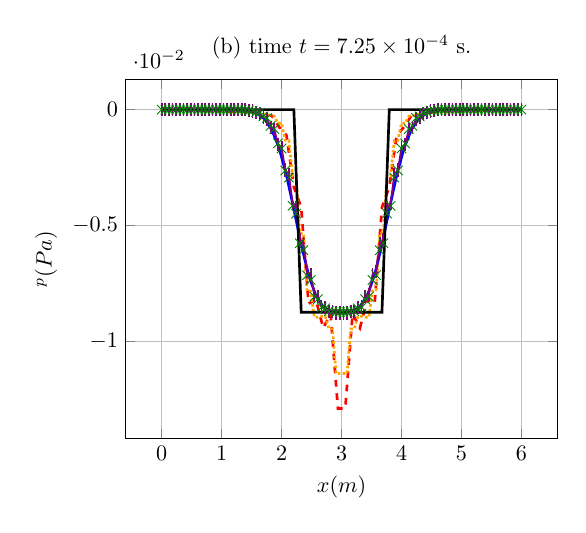
\begin{tikzpicture}[scale=0.8]
\begin{axis}[xlabel=$x (m)$,ylabel=$\eps^p (Pa)$,ymajorgrids=true,xmajorgrids=true,legend pos=outer north east,title={(b) time $t = 7.25\times 10^{-4} $ s.}]
\addplot[Red,very thick,mark=none,dashed,mark size=3pt] coordinates {(0.0,0.0) (0.12244897959183673,0.0) (0.24489795918367346,0.0) (0.36734693877551017,0.0) (0.4897959183673469,0.0) (0.6122448979591837,-3.577487902203997e-05) (0.7346938775510203,-6.306588245633642e-05) (0.8571428571428571,-6.949496312549484e-05) (0.9795918367346939,-8.005219978840035e-05) (1.1020408163265305,-9.009475914811774e-05) (1.2244897959183674,-9.858795071160678e-05) (1.346938775510204,-0.00010648019894997112) (1.4693877551020407,-0.00012616863649930955) (1.5918367346938775,-0.0001362011171739252) (1.7142857142857142,-0.00021257027814173217) (1.836734693877551,-0.00026486085096336456) (1.9591836734693877,-0.0007517028599145731) (2.0816326530612246,-0.0011133976998079925) (2.204081632653061,-0.003333993937447701) (2.326530612244898,-0.004209977621639336) (2.4489795918367347,-0.008357654568129739) (2.571428571428571,-0.00818541244484605) (2.693877551020408,-0.009408157524816411) (2.816326530612245,-0.008806354443804355) (2.9387755102040813,-0.012877303196726952) (3.061224489795918,-0.012877303196726607) (3.183673469387755,-0.008806354443804494) (3.306122448979592,-0.00940815752481628) (3.4285714285714284,-0.00818541244484614) (3.5510204081632653,-0.008357654568129634) (3.673469387755102,-0.004209977621639346) (3.7959183673469385,-0.0033339939374476507) (3.9183673469387754,-0.0011133976998079806) (4.040816326530612,-0.0007517028599145573) (4.163265306122449,-0.0002648608509633606) (4.285714285714286,-0.0002125702781417296) (4.408163265306122,-0.00013620111717393342) (4.530612244897959,-0.00012616863649931356) (4.653061224489796,-0.00010648019894998299) (4.775510204081632,-9.858795071160708e-05) (4.8979591836734695,-9.00947591481104e-05) (5.020408163265306,-8.005219978840008e-05) (5.142857142857142,-6.949496312550109e-05) (5.26530612244898,-6.306588245633955e-05) (5.387755102040816,-3.5774879022040825e-05) (5.5102040816326525,0.0) (5.63265306122449,0.0) (5.755102040816326,0.0) (5.877551020408163,0.0) (6.0,0.0) };
\addplot[Orange,very thick,mark=none,densely dotted,mark size=3pt] coordinates {(0.0,0.0) (0.06060606060606061,0.0) (0.12121212121212122,0.0) (0.18181818181818182,0.0) (0.24242424242424243,0.0) (0.30303030303030304,0.0) (0.36363636363636365,0.0) (0.42424242424242425,0.0) (0.48484848484848486,-1.3923950014088835e-06) (0.5454545454545454,-1.3923950014088835e-06) (0.6060606060606061,-4.802593874190819e-05) (0.6666666666666667,-4.802593874190819e-05) (0.7272727272727273,-6.41910410194221e-05) (0.7878787878787878,-6.41910410194221e-05) (0.8484848484848485,-6.859024545017706e-05) (0.9090909090909092,-6.859024545017706e-05) (0.9696969696969697,-7.288774581652991e-05) (1.0303030303030303,-7.288774581652991e-05) (1.0909090909090908,-8.507726423586093e-05) (1.1515151515151516,-8.507726423586093e-05) (1.2121212121212122,-9.691077127878779e-05) (1.2727272727272727,-9.691077127878779e-05) (1.3333333333333335,-0.0001071106301627928) (1.393939393939394,-0.0001071106301627928) (1.4545454545454546,-0.00011891582560129873) (1.5151515151515151,-0.00011891582560129873) (1.5757575757575757,-0.0001411626480808113) (1.6363636363636365,-0.0001411626480808113) (1.696969696969697,-0.00018474128224396107) (1.7575757575757576,-0.00018474128224396107) (1.8181818181818183,-0.00028928129016686006) (1.878787878787879,-0.00028928129016686006) (1.9393939393939394,-0.0005871331097401253) (2.0,-0.0005871331097401253) (2.0606060606060606,-0.0013271912464349832) (2.121212121212121,-0.0013271912464349832) (2.1818181818181817,-0.0028650643902802643) (2.2424242424242427,-0.0028650643902802643) (2.303030303030303,-0.005330257320518476) (2.3636363636363638,-0.005330257320518476) (2.4242424242424243,-0.007825827621282502) (2.484848484848485,-0.007825827621282502) (2.5454545454545454,-0.008947666418341944) (2.606060606060606,-0.008947666418341944) (2.666666666666667,-0.008904688564068288) (2.7272727272727275,-0.008904688564068288) (2.787878787878788,-0.00944634271615033) (2.8484848484848486,-0.00944634271615033) (2.909090909090909,-0.011373543353957122) (2.9696969696969697,-0.011373543353957122) (3.0303030303030303,-0.011373543353957112) (3.090909090909091,-0.011373543353957112) (3.1515151515151514,-0.009446342716150326) (3.2121212121212124,-0.009446342716150326) (3.272727272727273,-0.008904688564068298) (3.3333333333333335,-0.008904688564068298) (3.393939393939394,-0.008947666418341943) (3.4545454545454546,-0.008947666418341943) (3.515151515151515,-0.0078258276212825) (3.5757575757575757,-0.0078258276212825) (3.6363636363636367,-0.005330257320518468) (3.6969696969696972,-0.005330257320518468) (3.757575757575758,-0.002865064390280257) (3.8181818181818183,-0.002865064390280257) (3.878787878787879,-0.0013271912464349839) (3.9393939393939394,-0.0013271912464349839) (4.0,-0.0005871331097401301) (4.0606060606060606,-0.0005871331097401301) (4.121212121212121,-0.00028928129016686055) (4.181818181818182,-0.00028928129016686055) (4.242424242424242,-0.00018474128224395513) (4.303030303030303,-0.00018474128224395513) (4.363636363636363,-0.00014116264808081218) (4.424242424242425,-0.00014116264808081218) (4.484848484848485,-0.00011891582560129933) (4.545454545454546,-0.00011891582560129933) (4.606060606060606,-0.00010711063016279029) (4.666666666666667,-0.00010711063016279029) (4.7272727272727275,-9.691077127878893e-05) (4.787878787878788,-9.691077127878893e-05) (4.848484848484849,-8.507726423586494e-05) (4.909090909090909,-8.507726423586494e-05) (4.96969696969697,-7.288774581652709e-05) (5.03030303030303,-7.288774581652709e-05) (5.090909090909091,-6.859024545017819e-05) (5.151515151515151,-6.859024545017819e-05) (5.212121212121212,-6.419104101942352e-05) (5.2727272727272725,-6.419104101942352e-05) (5.333333333333334,-4.8025938741907344e-05) (5.3939393939393945,-4.8025938741907344e-05) (5.454545454545455,-1.3923950014085998e-06) (5.515151515151516,-1.3923950014085998e-06) (5.575757575757576,0.0) (5.636363636363637,0.0) (5.696969696969697,0.0) (5.757575757575758,0.0) (5.818181818181818,0.0) (5.878787878787879,0.0) (5.9393939393939394,0.0) (6.0,0.0) };
\addplot[Blue,very thick,mark=none,solid,mark size=3pt] coordinates {(0.0,-5.676632835751488e-19) (0.12244897959183673,-2.3898624238513766e-16) (0.24489795918367346,-3.735990751357306e-14) (0.36734693877551017,-2.3089144911084856e-12) (0.4897959183673469,-7.596762237094698e-11) (0.6122448979591837,-1.5415975357804979e-09) (0.7346938775510203,-1.0275730242331822e-08) (0.8571428571428571,-5.981932516353471e-08) (0.9795918367346939,-3.055798037968931e-07) (1.1020408163265305,-1.3747043608148892e-06) (1.2244897959183674,-5.4602719905226e-06) (1.346938775510204,-1.91823238251513e-05) (1.4693877551020407,-5.966726802674588e-05) (1.5918367346938775,-0.000164418651493838) (1.7142857142857142,-0.00040143744754996674) (1.836734693877551,-0.000868463225449077) (1.9591836734693877,-0.001665203797267752) (2.0816326530612246,-0.002832906100451628) (2.204081632653061,-0.004287995453610066) (2.326530612244898,-0.0058084443808726115) (2.4489795918367347,-0.007115753990208403) (2.571428571428571,-0.008016433919475449) (2.693877551020408,-0.008494471552590508) (2.816326530612245,-0.008677965053198252) (2.9387755102040813,-0.008723301560471332) (3.061224489795918,-0.008723301560471332) (3.183673469387755,-0.008677965053198252) (3.306122448979592,-0.00849447155259052) (3.4285714285714284,-0.008016433919475457) (3.5510204081632653,-0.007115753990208413) (3.673469387755102,-0.005808444380872623) (3.7959183673469385,-0.004287995453610076) (3.9183673469387754,-0.0028329061004516366) (4.040816326530612,-0.0016652037972677586) (4.163265306122449,-0.00086846322544908) (4.285714285714286,-0.0004014374475499613) (4.408163265306122,-0.00016441865149382611) (4.530612244897959,-5.9667268026732546e-05) (4.653061224489796,-1.918232382513086e-05) (4.775510204081632,-5.460271990507557e-06) (4.8979591836734695,-1.3747043608103478e-06) (5.020408163265306,-3.055798037929194e-07) (5.142857142857142,-5.981932515587126e-08) (5.26530612244898,-1.027573023324921e-08) (5.387755102040816,-1.5415975312391917e-09) (5.5102040816326525,-7.596762123562041e-11) (5.63265306122449,-2.308913923445202e-12) (5.755102040816326,-3.7358772187005907e-14) (5.877551020408163,-2.4097306387765065e-16) (6.0,-8.514949253627233e-19) };
\addplot[Purple,thick,mark=|,solid,mark size=3pt] coordinates {(0.0,0.0) (0.06060606060606061,0.0) (0.12121212121212122,0.0) (0.18181818181818182,0.0) (0.24242424242424243,0.0) (0.30303030303030304,0.0) (0.36363636363636365,0.0) (0.42424242424242425,0.0) (0.48484848484848486,0.0) (0.5454545454545454,0.0) (0.6060606060606061,0.0) (0.6666666666666667,0.0) (0.7272727272727273,0.0) (0.7878787878787878,0.0) (0.8484848484848485,0.0) (0.9090909090909092,0.0) (0.9696969696969697,0.0) (1.0303030303030303,0.0) (1.0909090909090908,0.0) (1.1515151515151516,-4.1375394533929374e-08) (1.2121212121212122,-1.6766275644359134e-07) (1.2727272727272727,-3.6899460485265364e-07) (1.3333333333333335,-3.7730684118324803e-06) (1.393939393939394,-6.566829345463855e-06) (1.4545454545454546,-3.9533489461271815e-05) (1.5151515151515151,-5.4725319017766484e-05) (1.5757575757575757,-0.0001393994522696901) (1.6363636363636365,-0.00016538778038305982) (1.696969696969697,-0.00034692599494932723) (1.7575757575757576,-0.0003991527105652267) (1.8181818181818183,-0.0007625905945333334) (1.878787878787879,-0.0008563059468014388) (1.9393939393939394,-0.0014922856868946723) (2.0,-0.0016374885246225213) (2.0606060606060606,-0.0025987877617010637) (2.121212121212121,-0.002790686204907401) (2.1818181818181817,-0.004030984098849627) (2.2424242424242427,-0.004243936219158137) (2.303030303030303,-0.0055885132243183545) (2.3636363636363638,-0.005782685656220611) (2.4242424242424243,-0.0069809715690837505) (2.484848484848485,-0.007121908461224029) (2.5454545454545454,-0.007972241161582445) (2.606060606060606,-0.008049596395188874) (2.666666666666667,-0.008505818537721688) (2.7272727272727275,-0.008534811001440776) (2.787878787878788,-0.008702033969468866) (2.8484848484848486,-0.008707545856799517) (2.909090909090909,-0.008758042662148493) (2.9696969696969697,-0.008762227333878615) (3.0303030303030303,-0.008762227333878615) (3.090909090909091,-0.008758042662148495) (3.1515151515151514,-0.008707545856799517) (3.2121212121212124,-0.008702033969468868) (3.272727272727273,-0.008534811001440776) (3.3333333333333335,-0.00850581853772169) (3.393939393939394,-0.008049596395188876) (3.4545454545454546,-0.007972241161582454) (3.515151515151515,-0.007121908461224033) (3.5757575757575757,-0.006980971569083754) (3.6363636363636367,-0.0057826856562206205) (3.6969696969696972,-0.005588513224318365) (3.757575757575758,-0.004243936219158141) (3.8181818181818183,-0.00403098409884963) (3.878787878787879,-0.0027906862049074093) (3.9393939393939394,-0.002598787761701072) (4.0,-0.0016374885246225263) (4.0606060606060606,-0.0014922856868946775) (4.121212121212121,-0.0008563059468014425) (4.181818181818182,-0.0007625905945333374) (4.242424242424242,-0.00039915271056523323) (4.303030303030303,-0.00034692599494933374) (4.363636363636363,-0.00016538778038306773) (4.424242424242425,-0.00013939945226969862) (4.484848484848485,-5.472531901777926e-05) (4.545454545454546,-3.9533489461283464e-05) (4.606060606060606,-6.566829345470383e-06) (4.666666666666667,-3.773068411838724e-06) (4.7272727272727275,-3.68994604853789e-07) (4.787878787878788,-1.6766275644359137e-07) (4.848484848484849,-4.1375394533929374e-08) (4.909090909090909,0.0) (4.96969696969697,0.0) (5.03030303030303,0.0) (5.090909090909091,0.0) (5.151515151515151,0.0) (5.212121212121212,0.0) (5.2727272727272725,0.0) (5.333333333333334,0.0) (5.3939393939393945,0.0) (5.454545454545455,0.0) (5.515151515151516,0.0) (5.575757575757576,0.0) (5.636363636363637,0.0) (5.696969696969697,0.0) (5.757575757575758,0.0) (5.818181818181818,0.0) (5.878787878787879,0.0) (5.9393939393939394,0.0) (6.0,0.0) };
\addplot[Green,thin,mark=x,only marks,mark size=3pt] coordinates {(0.0,-5.676632835751488e-19) (0.06060606060606061,0.0) (0.12121212121212122,-5.960464477539063e-18) (0.18181818181818182,-8.231117611839657e-18) (0.24242424242424243,-1.2593609946114675e-15) (0.30303030303030304,-2.566973368326823e-15) (0.36363636363636365,-1.2795357477097285e-13) (0.42424242424242425,-2.4569800921848845e-13) (0.48484848484848486,-6.614250512350173e-12) (0.5454545454545454,-1.1978970822833834e-11) (0.6060606060606061,-2.014539040270306e-10) (0.6666666666666667,-3.4473041437921067e-10) (0.7272727272727273,-1.7396754244963327e-09) (0.7878787878787878,-2.878236005703608e-09) (0.8484848484848485,-1.2915230488493328e-08) (0.9090909090909092,-2.0645992022468928e-08) (0.9696969696969697,-8.27788498841581e-08) (1.0303030303030303,-1.2777907757077899e-07) (1.0909090909090908,-4.594512838170642e-07) (1.1515151515151516,-6.844381126222156e-07) (1.2121212121212122,-2.2128580056431746e-06) (1.2727272727272727,-3.179616010181393e-06) (1.3333333333333335,-9.259748040896655e-06) (1.393939393939394,-1.2827869456145025e-05) (1.4545454545454546,-3.368426530185115e-05) (1.5151515151515151,-4.497549873773654e-05) (1.5757575757575757,-0.00010652981117383356) (1.6363636363636365,-0.0001370713310835756) (1.696969696969697,-0.00029284351963117065) (1.7575757575757576,-0.0003631417363302577) (1.8181818181818183,-0.0006995518818956783) (1.878787878787879,-0.0008364026933450982) (1.9393939393939394,-0.0014524891643318866) (2.0,-0.0016759867374438234) (2.0606060606060606,-0.002624841264006548) (2.121212121212121,-0.002927791589407064) (2.1818181818181817,-0.004143496150492473) (2.2424242424242427,-0.004479523423076173) (2.303030303030303,-0.00575685976116301) (2.3636363636363638,-0.006056043282157859) (2.4242424242424243,-0.007135597694533012) (2.484848484848485,-0.007343753961930436) (2.5454545454545454,-0.008058153161608643) (2.606060606060606,-0.008166928046930103) (2.666666666666667,-0.008522695893558911) (2.7272727272727275,-0.008562766723745093) (2.787878787878788,-0.008687900335388849) (2.8484848484848486,-0.008697160560944411) (2.909090909090909,-0.00872482225316362) (2.9696969696969697,-0.008725830219873004) (3.0303030303030303,-0.008725830219873004) (3.090909090909091,-0.00872482225316362) (3.1515151515151514,-0.008697160560944413) (3.2121212121212124,-0.008687900335388852) (3.272727272727273,-0.008562766723745095) (3.3333333333333335,-0.008522695893558915) (3.393939393939394,-0.008166928046930103) (3.4545454545454546,-0.008058153161608647) (3.515151515151515,-0.007343753961930437) (3.5757575757575757,-0.007135597694533014) (3.6363636363636367,-0.006056043282157861) (3.6969696969696972,-0.005756859761163013) (3.757575757575758,-0.004479523423076173) (3.8181818181818183,-0.004143496150492474) (3.878787878787879,-0.002927791589407064) (3.9393939393939394,-0.0026248412640065494) (4.0,-0.0016759867374438234) (4.0606060606060606,-0.0014524891643318892) (4.121212121212121,-0.0008364026933450992) (4.181818181818182,-0.0006995518818956805) (4.242424242424242,-0.00036314173633026085) (4.303030303030303,-0.0002928435196311738) (4.363636363636363,-0.00013707133108358015) (4.424242424242425,-0.00010652981117383724) (4.484848484848485,-4.497549873774307e-05) (4.545454545454546,-3.3684265301855976e-05) (4.606060606060606,-1.2827869456148999e-05) (4.666666666666667,-9.259748040899208e-06) (4.7272727272727275,-3.1796160101867863e-06) (4.787878787878788,-2.2128580056479997e-06) (4.848484848484849,-6.844381126324336e-07) (4.909090909090909,-4.5945128382728215e-07) (4.96969696969697,-1.277790775790101e-07) (5.03030303030303,-8.27788498932407e-08) (5.090909090909091,-2.0645992028145564e-08) (5.151515151515151,-1.2915230493318468e-08) (5.212121212121212,-2.878236009109588e-09) (5.2727272727272725,-1.7396754279023124e-09) (5.333333333333334,-3.4473041579836887e-10) (5.3939393939393945,-2.014539034593673e-10) (5.454545454545455,-1.1978968552180698e-11) (5.515151515151516,-6.614249377023606e-12) (5.575757575757576,-2.45694603238787e-13) (5.636363636363637,-1.2795045262291317e-13) (5.696969696969697,-2.566405705043248e-15) (5.757575757575758,-1.2633346375964938e-15) (5.818181818181818,-1.2772423880440849e-17) (5.878787878787879,-6.528127761114212e-18) (5.9393939393939394,0.0) (6.0,0.0) };
\addplot[black,very thick,mark=pentagone*,solid,mark size=3pt] coordinates {(0.0,-0.0) (0.12244897959183673,-0.0) (0.24489795918367346,-0.0) (0.36734693877551017,-0.0) (0.4897959183673469,-0.0) (0.6122448979591837,-0.0) (0.7346938775510203,-0.0) (0.8571428571428571,-0.0) (0.9795918367346939,-0.0) (1.1020408163265305,-0.0) (1.2244897959183674,-0.0) (1.346938775510204,-0.0) (1.4693877551020407,-0.0) (1.5918367346938775,-0.0) (1.7142857142857142,-0.0) (1.836734693877551,-0.0) (1.9591836734693877,-0.0) (2.0816326530612246,-0.0) (2.204081632653061,-0.0) (2.326530612244898,-0.008728715609439695) (2.4489795918367347,-0.008728715609439695) (2.571428571428571,-0.008728715609439695) (2.693877551020408,-0.008728715609439695) (2.816326530612245,-0.008728715609439695) (2.9387755102040813,-0.008728715609439695) (3.061224489795918,-0.008728715609439695) (3.183673469387755,-0.008728715609439695) (3.306122448979592,-0.008728715609439695) (3.4285714285714284,-0.008728715609439695) (3.5510204081632653,-0.008728715609439695) (3.673469387755102,-0.008728715609439695) (3.7959183673469385,-0.0) (3.9183673469387754,-0.0) (4.040816326530612,-0.0) (4.163265306122449,-0.0) (4.285714285714286,-0.0) (4.408163265306122,-0.0) (4.530612244897959,-0.0) (4.653061224489796,-0.0) (4.775510204081632,-0.0) (4.8979591836734695,-0.0) (5.020408163265306,-0.0) (5.142857142857142,-0.0) (5.26530612244898,-0.0) (5.387755102040816,-0.0) (5.5102040816326525,-0.0) (5.63265306122449,-0.0) (5.755102040816326,-0.0) (5.877551020408163,-0.0) (6.0,-0.0) };
%\legend{usl 1ppc,usl 2ppc,dgmpm 1ppc,dgmpm 2ppc,dgmpm 2ppc (RK2),exact}
\end{axis}
\end{tikzpicture}
%%% Local Variables:
%%% mode: latex
%%% TeX-master: "../../mainManuscript"
%%% End:
}
  {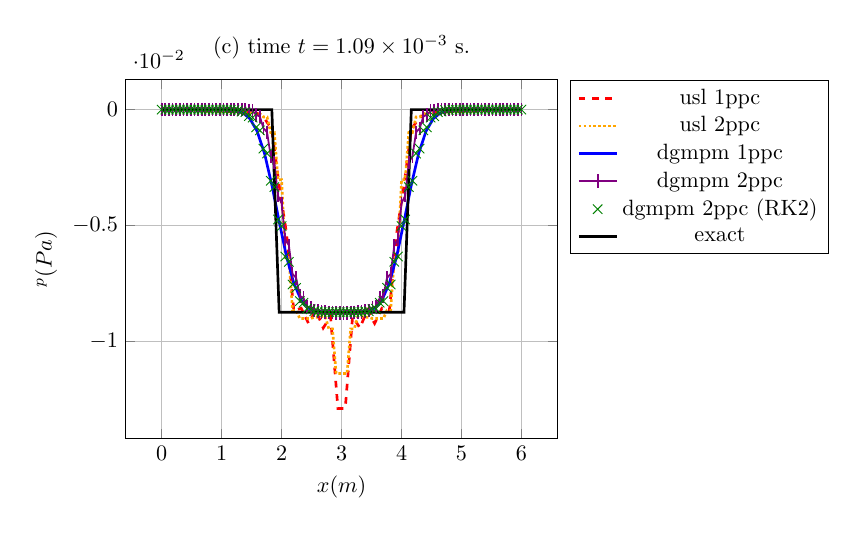
\begin{tikzpicture}[scale=0.8]
\begin{axis}[xlabel=$x (m)$,ylabel=$\eps^p (Pa)$,ymajorgrids=true,xmajorgrids=true,legend pos=outer north east,title={(c) time $t = 1.09\times 10^{-3} $ s.}]
\addplot[Red,very thick,mark=none,dashed,mark size=3pt] coordinates {(0.0,0.0) (0.12244897959183673,0.0) (0.24489795918367346,0.0) (0.36734693877551017,0.0) (0.4897959183673469,0.0) (0.6122448979591837,-3.577487902203997e-05) (0.7346938775510203,-6.306588245633642e-05) (0.8571428571428571,-6.949496312549484e-05) (0.9795918367346939,-8.005219978840035e-05) (1.1020408163265305,-9.009475914811774e-05) (1.2244897959183674,-9.858795071160678e-05) (1.346938775510204,-0.00010648019894997112) (1.4693877551020407,-0.00013090237763271645) (1.5918367346938775,-0.00015585484694440393) (1.7142857142857142,-0.00037807434010367157) (1.836734693877551,-0.0008542508721889013) (1.9591836734693877,-0.003265580636192999) (2.0816326530612246,-0.005332403663610279) (2.204081632653061,-0.008685547798871193) (2.326530612244898,-0.008557827562005196) (2.4489795918367347,-0.009212270529983918) (2.571428571428571,-0.008640321746270047) (2.693877551020408,-0.009408157524816411) (2.816326530612245,-0.008914806029937274) (2.9387755102040813,-0.012877303196726952) (3.061224489795918,-0.012877303196726607) (3.183673469387755,-0.008914806029937388) (3.306122448979592,-0.00940815752481628) (3.4285714285714284,-0.008640321746270135) (3.5510204081632653,-0.009212270529983827) (3.673469387755102,-0.008557827562005267) (3.7959183673469385,-0.008685547798871113) (3.9183673469387754,-0.005332403663610266) (4.040816326530612,-0.003265580636192934) (4.163265306122449,-0.0008542508721888987) (4.285714285714286,-0.00037807434010366447) (4.408163265306122,-0.00015585484694441217) (4.530612244897959,-0.00013090237763272187) (4.653061224489796,-0.00010648019894998299) (4.775510204081632,-9.858795071160708e-05) (4.8979591836734695,-9.00947591481104e-05) (5.020408163265306,-8.005219978840008e-05) (5.142857142857142,-6.949496312550109e-05) (5.26530612244898,-6.306588245633955e-05) (5.387755102040816,-3.5774879022040825e-05) (5.5102040816326525,0.0) (5.63265306122449,0.0) (5.755102040816326,0.0) (5.877551020408163,0.0) (6.0,0.0) };
\addplot[Orange,very thick,mark=none,densely dotted,mark size=3pt] coordinates {(0.0,0.0) (0.06060606060606061,0.0) (0.12121212121212122,0.0) (0.18181818181818182,0.0) (0.24242424242424243,0.0) (0.30303030303030304,0.0) (0.36363636363636365,0.0) (0.42424242424242425,0.0) (0.48484848484848486,-1.3923950014088835e-06) (0.5454545454545454,-1.3923950014088835e-06) (0.6060606060606061,-4.802593874190819e-05) (0.6666666666666667,-4.802593874190819e-05) (0.7272727272727273,-6.41910410194221e-05) (0.7878787878787878,-6.41910410194221e-05) (0.8484848484848485,-6.859024545017706e-05) (0.9090909090909092,-6.859024545017706e-05) (0.9696969696969697,-7.288774581652991e-05) (1.0303030303030303,-7.288774581652991e-05) (1.0909090909090908,-8.507726423586093e-05) (1.1515151515151516,-8.507726423586093e-05) (1.2121212121212122,-9.691077127878779e-05) (1.2727272727272727,-9.691077127878779e-05) (1.3333333333333335,-0.00010711649363712468) (1.393939393939394,-0.00010711649363712468) (1.4545454545454546,-0.00012487268940087668) (1.5151515151515151,-0.00012487268940087668) (1.5757575757575757,-0.00016846150368530778) (1.6363636363636365,-0.00016846150368530778) (1.696969696969697,-0.00032141238951341054) (1.7575757575757576,-0.00032141238951341054) (1.8181818181818183,-0.0009863835722303473) (1.878787878787879,-0.0009863835722303473) (1.9393939393939394,-0.003025063907376677) (2.0,-0.003025063907376677) (2.0606060606060606,-0.006366348809033719) (2.121212121212121,-0.006366348809033719) (2.1818181818181817,-0.008647239978151484) (2.2424242424242427,-0.008647239978151484) (2.303030303030303,-0.009001860585213824) (2.3636363636363638,-0.009001860585213824) (2.4242424242424243,-0.009001507335175213) (2.484848484848485,-0.009001507335175213) (2.5454545454545454,-0.008949274888554966) (2.606060606060606,-0.008949274888554966) (2.666666666666667,-0.00891581762874243) (2.7272727272727275,-0.00891581762874243) (2.787878787878788,-0.00944634271615033) (2.8484848484848486,-0.00944634271615033) (2.909090909090909,-0.011373543353957122) (2.9696969696969697,-0.011373543353957122) (3.0303030303030303,-0.011373543353957112) (3.090909090909091,-0.011373543353957112) (3.1515151515151514,-0.009446342716150326) (3.2121212121212124,-0.009446342716150326) (3.272727272727273,-0.00891581762874244) (3.3333333333333335,-0.00891581762874244) (3.393939393939394,-0.008949274888554966) (3.4545454545454546,-0.008949274888554966) (3.515151515151515,-0.009001507335175215) (3.5757575757575757,-0.009001507335175215) (3.6363636363636367,-0.009001860585213826) (3.6969696969696972,-0.009001860585213826) (3.757575757575758,-0.008647239978151493) (3.8181818181818183,-0.008647239978151493) (3.878787878787879,-0.006366348809033716) (3.9393939393939394,-0.006366348809033716) (4.0,-0.003025063907376669) (4.0606060606060606,-0.003025063907376669) (4.121212121212121,-0.0009863835722303564) (4.181818181818182,-0.0009863835722303564) (4.242424242424242,-0.00032141238951339976) (4.303030303030303,-0.00032141238951339976) (4.363636363636363,-0.00016846150368530894) (4.424242424242425,-0.00016846150368530894) (4.484848484848485,-0.00012487268940087758) (4.545454545454546,-0.00012487268940087758) (4.606060606060606,-0.00010711649363712272) (4.666666666666667,-0.00010711649363712272) (4.7272727272727275,-9.691077127878893e-05) (4.787878787878788,-9.691077127878893e-05) (4.848484848484849,-8.507726423586494e-05) (4.909090909090909,-8.507726423586494e-05) (4.96969696969697,-7.288774581652709e-05) (5.03030303030303,-7.288774581652709e-05) (5.090909090909091,-6.859024545017819e-05) (5.151515151515151,-6.859024545017819e-05) (5.212121212121212,-6.419104101942352e-05) (5.2727272727272725,-6.419104101942352e-05) (5.333333333333334,-4.8025938741907344e-05) (5.3939393939393945,-4.8025938741907344e-05) (5.454545454545455,-1.3923950014085998e-06) (5.515151515151516,-1.3923950014085998e-06) (5.575757575757576,0.0) (5.636363636363637,0.0) (5.696969696969697,0.0) (5.757575757575758,0.0) (5.818181818181818,0.0) (5.878787878787879,0.0) (5.9393939393939394,0.0) (6.0,0.0) };
\addplot[Blue,very thick,mark=none,solid,mark size=3pt] coordinates {(0.0,-5.676632835751488e-19) (0.12244897959183673,-2.3898624238513766e-16) (0.24489795918367346,-3.735990751357306e-14) (0.36734693877551017,-2.3089144911084856e-12) (0.4897959183673469,-7.596762237094698e-11) (0.6122448979591837,-1.5415975357804979e-09) (0.7346938775510203,-2.1087029002110162e-08) (0.8571428571428571,-2.0628580472526095e-07) (0.9795918367346939,-1.5051975779320511e-06) (1.1020408163265305,-8.452232526292688e-06) (1.2244897959183674,-3.741900938747327e-05) (1.346938775510204,-0.00013315210803806102) (1.4693877551020407,-0.00038701776930482674) (1.5918367346938775,-0.0009319386970470464) (1.7142857142857142,-0.0018842066770200564) (1.836734693877551,-0.0032431409441831516) (1.9591836734693877,-0.004827293901207316) (2.0816326530612246,-0.00633202118341673) (2.204081632653061,-0.007489880430691718) (2.326530612244898,-0.008204526972019307) (2.4489795918367347,-0.008552921390073501) (2.571428571428571,-0.008674876019514461) (2.693877551020408,-0.008716486656783273) (2.816326530612245,-0.008726887116624966) (2.9387755102040813,-0.008728580772745199) (3.061224489795918,-0.008728580772745199) (3.183673469387755,-0.008726887116624966) (3.306122448979592,-0.00871648665678328) (3.4285714285714284,-0.008674876019514466) (3.5510204081632653,-0.008552921390073511) (3.673469387755102,-0.008204526972019318) (3.7959183673469385,-0.007489880430691721) (3.9183673469387754,-0.00633202118341673) (4.040816326530612,-0.0048272939012073204) (4.163265306122449,-0.0032431409441831525) (4.285714285714286,-0.001884206677020053) (4.408163265306122,-0.0009319386970470392) (4.530612244897959,-0.0003870177693048181) (4.653061224489796,-0.0001331521080380519) (4.775510204081632,-3.7419009387462476e-05) (4.8979591836734695,-8.452232526284741e-06) (5.020408163265306,-1.5051975779246716e-06) (5.142857142857142,-2.0628580471617835e-07) (5.26530612244898,-2.1087028991608393e-08) (5.387755102040816,-1.5415975312391917e-09) (5.5102040816326525,-7.596762123562041e-11) (5.63265306122449,-2.308913923445202e-12) (5.755102040816326,-3.7358772187005907e-14) (5.877551020408163,-2.4097306387765065e-16) (6.0,-8.514949253627233e-19) };
\addplot[Purple,thick,mark=|,solid,mark size=3pt] coordinates {(0.0,0.0) (0.06060606060606061,0.0) (0.12121212121212122,0.0) (0.18181818181818182,0.0) (0.24242424242424243,0.0) (0.30303030303030304,0.0) (0.36363636363636365,0.0) (0.42424242424242425,0.0) (0.48484848484848486,0.0) (0.5454545454545454,0.0) (0.6060606060606061,0.0) (0.6666666666666667,0.0) (0.7272727272727273,0.0) (0.7878787878787878,0.0) (0.8484848484848485,0.0) (0.9090909090909092,0.0) (0.9696969696969697,0.0) (1.0303030303030303,0.0) (1.0909090909090908,0.0) (1.1515151515151516,-4.1375394533929374e-08) (1.2121212121212122,-1.6766275644359134e-07) (1.2727272727272727,-3.6899460485265364e-07) (1.3333333333333335,-3.7730684118324803e-06) (1.393939393939394,-6.566829345463855e-06) (1.4545454545454546,-3.9533489461271815e-05) (1.5151515151515151,-5.787873091723124e-05) (1.5757575757575757,-0.0002274525995650831) (1.6363636363636365,-0.00029636567097843057) (1.696969696969697,-0.0008043486101741406) (1.7575757575757576,-0.0009756904136278646) (1.8181818181818183,-0.002007506978689405) (1.878787878787879,-0.0022778320644552875) (1.9393939393939394,-0.0037101075201987303) (2.0,-0.004034858131037031) (2.0606060606060606,-0.005583330117719787) (2.121212121212121,-0.005852176347303774) (2.1818181818181817,-0.007081628136433296) (2.2424242424242427,-0.007249585758095964) (2.303030303030303,-0.008025296353006806) (2.3636363636363638,-0.008110184081085586) (2.4242424242424243,-0.008492622343293309) (2.484848484848485,-0.008525512701242518) (2.5454545454545454,-0.008671015536515168) (2.606060606060606,-0.008680086368368912) (2.666666666666667,-0.008720691408181637) (2.7272727272727275,-0.008722186625565662) (2.787878787878788,-0.00872959098319658) (2.8484848484848486,-0.008729715721981647) (2.909090909090909,-0.008758042662148493) (2.9696969696969697,-0.008762227333878615) (3.0303030303030303,-0.008762227333878615) (3.090909090909091,-0.008758042662148495) (3.1515151515151514,-0.008729715721981645) (3.2121212121212124,-0.008729590983196582) (3.272727272727273,-0.008722186625565662) (3.3333333333333335,-0.008720691408181639) (3.393939393939394,-0.00868008636836891) (3.4545454545454546,-0.008671015536515165) (3.515151515151515,-0.008525512701242514) (3.5757575757575757,-0.008492622343293309) (3.6363636363636367,-0.00811018408108559) (3.6969696969696972,-0.008025296353006812) (3.757575757575758,-0.007249585758095969) (3.8181818181818183,-0.0070816281364333026) (3.878787878787879,-0.005852176347303775) (3.9393939393939394,-0.005583330117719789) (4.0,-0.0040348581310370385) (4.0606060606060606,-0.0037101075201987394) (4.121212121212121,-0.0022778320644552983) (4.181818181818182,-0.002007506978689416) (4.242424242424242,-0.0009756904136278739) (4.303030303030303,-0.0008043486101741499) (4.363636363636363,-0.00029636567097843854) (4.424242424242425,-0.00022745259956509018) (4.484848484848485,-5.787873091724344e-05) (4.545454545454546,-3.9533489461283464e-05) (4.606060606060606,-6.566829345470383e-06) (4.666666666666667,-3.773068411838724e-06) (4.7272727272727275,-3.68994604853789e-07) (4.787878787878788,-1.6766275644359137e-07) (4.848484848484849,-4.1375394533929374e-08) (4.909090909090909,0.0) (4.96969696969697,0.0) (5.03030303030303,0.0) (5.090909090909091,0.0) (5.151515151515151,0.0) (5.212121212121212,0.0) (5.2727272727272725,0.0) (5.333333333333334,0.0) (5.3939393939393945,0.0) (5.454545454545455,0.0) (5.515151515151516,0.0) (5.575757575757576,0.0) (5.636363636363637,0.0) (5.696969696969697,0.0) (5.757575757575758,0.0) (5.818181818181818,0.0) (5.878787878787879,0.0) (5.9393939393939394,0.0) (6.0,0.0) };
\addplot[Green,thin,mark=x,only marks,mark size=3pt] coordinates {(0.0,-5.676632835751488e-19) (0.06060606060606061,0.0) (0.12121212121212122,-5.960464477539063e-18) (0.18181818181818182,-8.231117611839657e-18) (0.24242424242424243,-1.2593609946114675e-15) (0.30303030303030304,-2.566973368326823e-15) (0.36363636363636365,-1.2795357477097285e-13) (0.42424242424242425,-2.4569800921848845e-13) (0.48484848484848486,-6.614250512350173e-12) (0.5454545454545454,-1.1978970822833834e-11) (0.6060606060606061,-2.014539040270306e-10) (0.6666666666666667,-3.4473041437921067e-10) (0.7272727272727273,-3.958928195919309e-09) (0.7878787878787878,-6.412620588143667e-09) (0.8484848484848485,-5.3364499986455554e-08) (0.9090909090909092,-8.197237874269486e-08) (0.9696969696969697,-5.155914888793514e-07) (1.0303030303030303,-7.524956608332339e-07) (1.0909090909090908,-3.6911086009462675e-06) (1.1515151515151516,-5.128586973845675e-06) (1.2121212121212122,-2.0096823934549662e-05) (1.2727272727272727,-2.6639006500208663e-05) (1.3333333333333335,-8.500574414884647e-05) (1.393939393939394,-0.00010773647495164076) (1.4545454545454546,-0.00028442785366869175) (1.5151515151515151,-0.0003455251868600774) (1.5757575757575757,-0.0007651640013258602) (1.6363636363636365,-0.0008934272034897002) (1.696969696969697,-0.0016811593270009762) (1.7575757575757576,-0.001892798143971582) (1.8181818181818183,-0.0030669939640570066) (1.878787878787879,-0.0033423564247713746) (1.9393939393939394,-0.004734809703010922) (2.0,-0.005017334536365495) (2.0606060606060606,-0.006329679309076545) (2.121212121212121,-0.006557472732041174) (2.1818181818181817,-0.007536143497329047) (2.2424242424242427,-0.007679356454328646) (2.303030303030303,-0.00825193835878759) (2.3636363636363638,-0.008321206280476908) (2.4242424242424243,-0.008580337649446788) (2.484848484848485,-0.008605558443364046) (2.5454545454545454,-0.008686715531944143) (2.606060606060606,-0.008694798692719908) (2.666666666666667,-0.008720028673057422) (2.7272727272727275,-0.008721895117205144) (2.787878787878788,-0.008727550668862797) (2.8484848484848486,-0.008727826804119215) (2.909090909090909,-0.00872863974231939) (2.9696969696969697,-0.008728659383864157) (3.0303030303030303,-0.008728659383864159) (3.090909090909091,-0.008728639742319392) (3.1515151515151514,-0.008727826804119217) (3.2121212121212124,-0.008727550668862803) (3.272727272727273,-0.008721895117205145) (3.3333333333333335,-0.008720028673057423) (3.393939393939394,-0.008694798692719906) (3.4545454545454546,-0.008686715531944143) (3.515151515151515,-0.008605558443364044) (3.5757575757575757,-0.008580337649446788) (3.6363636363636367,-0.008321206280476912) (3.6969696969696972,-0.008251938358787594) (3.757575757575758,-0.007679356454328649) (3.8181818181818183,-0.0075361434973290516) (3.878787878787879,-0.006557472732041174) (3.9393939393939394,-0.006329679309076547) (4.0,-0.005017334536365494) (4.0606060606060606,-0.004734809703010924) (4.121212121212121,-0.0033423564247713777) (4.181818181818182,-0.0030669939640570088) (4.242424242424242,-0.0018927981439715827) (4.303030303030303,-0.001681159327000978) (4.363636363636363,-0.0008934272034897071) (4.424242424242425,-0.0007651640013258641) (4.484848484848485,-0.00034552518686008227) (4.545454545454546,-0.00028442785366869516) (4.606060606060606,-0.00010773647495164786) (4.666666666666667,-8.500574414885329e-05) (4.7272727272727275,-2.6639006500214904e-05) (4.787878787878788,-2.009682393455562e-05) (4.848484848484849,-5.1285869738558925e-06) (4.909090909090909,-3.6911086009562015e-06) (4.96969696969697,-7.524956608437356e-07) (5.03030303030303,-5.155914888895694e-07) (5.090909090909091,-8.197237874439784e-08) (5.151515151515151,-5.336449998730705e-08) (5.212121212121212,-6.412620592684973e-09) (5.2727272727272725,-3.958928200460616e-09) (5.333333333333334,-3.4473041579836887e-10) (5.3939393939393945,-2.014539034593673e-10) (5.454545454545455,-1.1978968552180698e-11) (5.515151515151516,-6.614249377023606e-12) (5.575757575757576,-2.45694603238787e-13) (5.636363636363637,-1.2795045262291317e-13) (5.696969696969697,-2.566405705043248e-15) (5.757575757575758,-1.2633346375964938e-15) (5.818181818181818,-1.2772423880440849e-17) (5.878787878787879,-6.528127761114212e-18) (5.9393939393939394,0.0) (6.0,0.0) };
\addplot[black,very thick,mark=pentagone*,solid,mark size=3pt] coordinates {(0.0,-0.0) (0.12244897959183673,-0.0) (0.24489795918367346,-0.0) (0.36734693877551017,-0.0) (0.4897959183673469,-0.0) (0.6122448979591837,-0.0) (0.7346938775510203,-0.0) (0.8571428571428571,-0.0) (0.9795918367346939,-0.0) (1.1020408163265305,-0.0) (1.2244897959183674,-0.0) (1.346938775510204,-0.0) (1.4693877551020407,-0.0) (1.5918367346938775,-0.0) (1.7142857142857142,-0.0) (1.836734693877551,-0.0) (1.9591836734693877,-0.008728715609439695) (2.0816326530612246,-0.008728715609439695) (2.204081632653061,-0.008728715609439695) (2.326530612244898,-0.008728715609439695) (2.4489795918367347,-0.008728715609439695) (2.571428571428571,-0.008728715609439695) (2.693877551020408,-0.008728715609439695) (2.816326530612245,-0.008728715609439695) (2.9387755102040813,-0.008728715609439695) (3.061224489795918,-0.008728715609439695) (3.183673469387755,-0.008728715609439695) (3.306122448979592,-0.008728715609439695) (3.4285714285714284,-0.008728715609439695) (3.5510204081632653,-0.008728715609439695) (3.673469387755102,-0.008728715609439695) (3.7959183673469385,-0.008728715609439695) (3.9183673469387754,-0.008728715609439695) (4.040816326530612,-0.008728715609439695) (4.163265306122449,-0.0) (4.285714285714286,-0.0) (4.408163265306122,-0.0) (4.530612244897959,-0.0) (4.653061224489796,-0.0) (4.775510204081632,-0.0) (4.8979591836734695,-0.0) (5.020408163265306,-0.0) (5.142857142857142,-0.0) (5.26530612244898,-0.0) (5.387755102040816,-0.0) (5.5102040816326525,-0.0) (5.63265306122449,-0.0) (5.755102040816326,-0.0) (5.877551020408163,-0.0) (6.0,-0.0) };
\legend{usl 1ppc,usl 2ppc,dgmpm 1ppc,dgmpm 2ppc,dgmpm 2ppc (RK2),exact}
\end{axis}
\end{tikzpicture}
%%% Local Variables:
%%% mode: latex
%%% TeX-master: "../../mainManuscript"
%%% End:
}
  \caption{elastic-plastic RP epsp}
  \label{fig:epsp_elastoplastic_RP}
\end{figure}


Comparison with fvm and FEM (lumped mass matrix + radial return for integrating constitutive equations)
\begin{figure}[h!]
  \centering
  {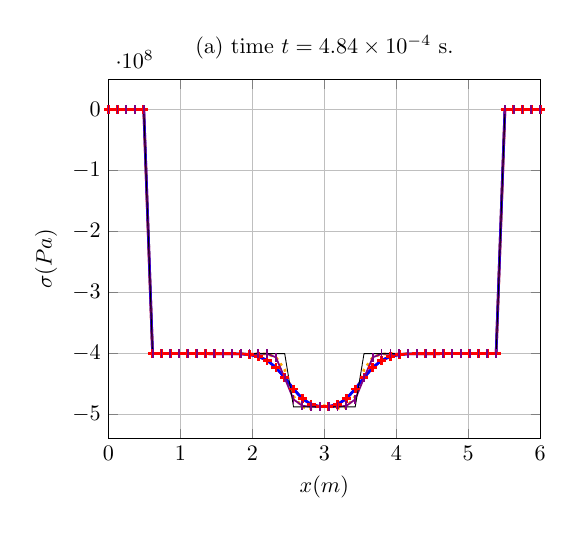
\begin{tikzpicture}[scale=0.8]
\begin{axis}[xlabel=$x (m)$,ylabel=$\sigma (Pa)$,ymajorgrids=true,xmajorgrids=true,legend pos=outer north east,title={(a) time $t = 4.84\times 10^{-4} $ s.},xmin=0.,xmax=6.]
\addplot[Red,very thick,mark=+,solid] coordinates {(0.0,-1.4032094709741823e-07) (0.12244897959183673,1.4032094709741797e-07) (0.24489795918367346,-5.501313561848306e-23) (0.36734693877551017,-1.4032094709741882e-07) (0.4897959183673469,-4.2096284129225576e-07) (0.6122448979591837,-400000000.0000052) (0.7346938775510203,-400000000.0003803) (0.8571428571428571,-400000000.0131417) (0.9795918367346939,-400000000.2874559) (1.1020408163265305,-400000004.46415013) (1.2244897959183674,-400000052.34678423) (1.346938775510204,-400000481.2046858) (1.4693877551020407,-400003554.03647596) (1.5918367346938775,-400021443.0967657) (1.7142857142857142,-400106894.9802318) (1.836734693877551,-400443646.6051052) (1.9591836734693877,-401540408.59283984) (2.0816326530612246,-404487333.2231472) (2.204081632653061,-410984305.87262785) (2.326530612244898,-422622254.02503896) (2.4489795918367347,-439299786.1010327) (2.571428571428571,-457971198.93456453) (2.693877551020408,-473710434.18348145) (2.816326530612245,-483108267.7934754) (2.9387755102040813,-486652315.1909913) (3.061224489795918,-486652315.1909913) (3.183673469387755,-483108267.7934754) (3.306122448979592,-473710434.18348145) (3.4285714285714284,-457971198.93456453) (3.5510204081632653,-439299786.1010328) (3.673469387755102,-422622254.025039) (3.7959183673469385,-410984305.8726279) (3.9183673469387754,-404487333.2231472) (4.040816326530612,-401540408.59283984) (4.163265306122449,-400443646.6051051) (4.285714285714286,-400106894.98023176) (4.408163265306122,-400021443.0967656) (4.530612244897959,-400003554.0364758) (4.653061224489796,-400000481.20468575) (4.775510204081632,-400000052.3467841) (4.8979591836734695,-400000004.46415013) (5.020408163265306,-400000000.2874559) (5.142857142857142,-400000000.01314175) (5.26530612244898,-400000000.0003803) (5.387755102040816,-400000000.0000052) (5.5102040816326525,1.403209470974181e-07) (5.63265306122449,-4.209628412922546e-07) (5.755102040816326,-7.335084749131074e-23) (5.877551020408163,-7.335084749131074e-23) (6.0,1.4032094709741816e-07) };
\addplot[Orange,very thick,mark=none,dotted] coordinates {(0.0011999999999999927,0.0) (0.12359999999999997,0.0) (0.24599999999999994,0.0) (0.36839999999999995,0.0) (0.4907999999999999,0.0) (0.6131999999999999,-399999999.9999996) (0.7355999999999999,-399999999.9999968) (0.858,-400000000.0) (0.9803999999999998,-399999999.9999996) (1.1027999999999998,-400000000.00000036) (1.2251999999999996,-400000000.0000013) (1.3475999999999997,-400000000.0000979) (1.4699999999999998,-400000000.00582314) (1.5923999999999996,-400000000.2649425) (1.7147999999999997,-400000009.2416795) (1.8371999999999995,-400000245.9026529) (1.9595999999999996,-400004932.9535555) (2.0819999999999994,-400073165.4563783) (2.2043999999999997,-400778734.27312934) (2.3267999999999995,-405684157.67745835) (2.4491999999999994,-426483554.2497189) (2.5715999999999997,-469882444.732417) (2.6939999999999995,-487460509.8573178) (2.8163999999999993,-489834934.6920107) (2.9387999999999996,-485390329.82597953) (3.0611999999999995,-485390329.8259847) (3.1835999999999993,-489834934.692009) (3.305999999999999,-487460509.85731673) (3.4283999999999994,-469882444.73241717) (3.5507999999999993,-426483554.2497191) (3.673199999999999,-405684157.67745817) (3.7955999999999994,-400778734.27312946) (3.9179999999999993,-400073165.4563784) (4.040399999999999,-400004932.95355564) (4.1628,-400000245.9026529) (4.2852,-400000009.2416795) (4.4076,-400000000.2649422) (4.53,-400000000.00582296) (4.6524,-400000000.0000977) (4.7748,-400000000.0000014) (4.8972,-400000000.00000036) (5.0196,-399999999.9999973) (5.142,-400000000.0) (5.2644,-400000000.0) (5.3868,-399999999.9999975) (5.5092,0.0) (5.6316,0.0) (5.754,0.0) (5.8764,0.0) (5.9988,0.0) };
\addplot[Blue,very thick,mark=none,solid] coordinates {(0.0011999999999999927,0.0) (0.12359999999999997,0.0) (0.24599999999999994,0.0) (0.36839999999999995,0.0) (0.4907999999999999,0.0) (0.6131999999999999,-400000000.0000052) (0.7355999999999999,-400000000.0003801) (0.858,-400000000.01314163) (0.9803999999999998,-400000000.2874559) (1.1027999999999998,-400000004.46415013) (1.2251999999999996,-400000052.3467841) (1.3475999999999997,-400000481.20468575) (1.4699999999999998,-400003554.03647584) (1.5923999999999996,-400021443.0967656) (1.7147999999999997,-400106894.9802317) (1.8371999999999995,-400443646.6051051) (1.9595999999999996,-401540408.5928399) (2.0819999999999994,-404487333.2231473) (2.2043999999999997,-410984305.8726279) (2.3267999999999995,-422622254.0250391) (2.4491999999999994,-439299786.10103285) (2.5715999999999997,-457971198.9345646) (2.6939999999999995,-473710434.1834816) (2.8163999999999993,-483108267.79347533) (2.9387999999999996,-486652315.1909914) (3.0611999999999995,-486652315.1909914) (3.1835999999999993,-483108267.79347533) (3.305999999999999,-473710434.1834816) (3.4283999999999994,-457971198.9345646) (3.5507999999999993,-439299786.10103285) (3.673199999999999,-422622254.0250391) (3.7955999999999994,-410984305.8726279) (3.9179999999999993,-404487333.2231473) (4.040399999999999,-401540408.5928399) (4.1628,-400443646.6051051) (4.2852,-400106894.9802317) (4.4076,-400021443.0967656) (4.53,-400003554.03647584) (4.6524,-400000481.20468575) (4.7748,-400000052.3467841) (4.8972,-400000004.46415013) (5.0196,-400000000.2874559) (5.142,-400000000.01314163) (5.2644,-400000000.0003801) (5.3868,-400000000.0000052) (5.5092,0.0) (5.6316,0.0) (5.754,0.0) (5.8764,0.0) (5.9988,0.0) };
\addplot[Purple,thick,mark=|,solid] coordinates {(0.0011999999999999927,0.0) (0.12359999999999997,0.0) (0.24599999999999994,0.0) (0.36839999999999995,0.0) (0.4907999999999999,0.0) (0.6131999999999999,-399999999.99999994) (0.7355999999999999,-400000000.0) (0.858,-400000000.0) (0.9803999999999998,-400000000.0) (1.1027999999999998,-400000000.0) (1.2251999999999996,-400000000.00000024) (1.3475999999999997,-400000000.00001407) (1.4699999999999998,-400000000.0007095) (1.5923999999999996,-400000000.0295273) (1.7147999999999997,-400000001.0283913) (1.8371999999999995,-400000030.33246076) (1.9595999999999996,-400000768.4378232) (2.0819999999999994,-400016975.1308303) (2.2043999999999997,-400318783.1149349) (2.3267999999999995,-405939608.94153374) (2.4491999999999994,-439871901.51192373) (2.5715999999999997,-475012040.0305417) (2.6939999999999995,-485411927.60231024) (2.8163999999999993,-487101987.7579666) (2.9387999999999996,-487278357.03341293) (3.0611999999999995,-487278357.03341293) (3.1835999999999993,-487101987.7579666) (3.305999999999999,-485411927.60231024) (3.4283999999999994,-475012040.0305417) (3.5507999999999993,-439871901.51192373) (3.673199999999999,-405939608.94153374) (3.7955999999999994,-400318783.1149349) (3.9179999999999993,-400016975.1308303) (4.040399999999999,-400000768.4378232) (4.1628,-400000030.33246076) (4.2852,-400000001.0283913) (4.4076,-400000000.0295273) (4.53,-400000000.0007095) (4.6524,-400000000.00001407) (4.7748,-400000000.0000003) (4.8972,-400000000.0) (5.0196,-400000000.0) (5.142,-400000000.0) (5.2644,-400000000.0) (5.3868,-399999999.99999994) (5.5092,0.0) (5.6316,0.0) (5.754,0.0) (5.8764,0.0) (5.9988,0.0) };
\addplot[black,thin,mark=none,solid] coordinates {(0.0,-0.0) (0.12244897959183673,-0.0) (0.24489795918367346,-0.0) (0.36734693877551017,-0.0) (0.4897959183673469,-0.0) (0.6122448979591837,-400000000.0) (0.7346938775510203,-400000000.0) (0.8571428571428571,-400000000.0) (0.9795918367346939,-400000000.0) (1.1020408163265305,-400000000.0) (1.2244897959183674,-400000000.0) (1.346938775510204,-400000000.0) (1.4693877551020407,-400000000.0) (1.5918367346938775,-400000000.0) (1.7142857142857142,-400000000.0) (1.836734693877551,-400000000.0) (1.9591836734693877,-400000000.0) (2.0816326530612246,-400000000.0) (2.204081632653061,-400000000.0) (2.326530612244898,-400000000.0) (2.4489795918367347,-400000000.0) (2.571428571428571,-487287156.09439695) (2.693877551020408,-487287156.09439695) (2.816326530612245,-487287156.09439695) (2.9387755102040813,-487287156.09439695) (3.061224489795918,-487287156.09439695) (3.183673469387755,-487287156.09439695) (3.306122448979592,-487287156.09439695) (3.4285714285714284,-487287156.09439695) (3.5510204081632653,-400000000.0) (3.673469387755102,-400000000.0) (3.7959183673469385,-400000000.0) (3.9183673469387754,-400000000.0) (4.040816326530612,-400000000.0) (4.163265306122449,-400000000.0) (4.285714285714286,-400000000.0) (4.408163265306122,-400000000.0) (4.530612244897959,-400000000.0) (4.653061224489796,-400000000.0) (4.775510204081632,-400000000.0) (4.8979591836734695,-400000000.0) (5.020408163265306,-400000000.0) (5.142857142857142,-400000000.0) (5.26530612244898,-400000000.0) (5.387755102040816,-400000000.0) (5.5102040816326525,-0.0) (5.63265306122449,-0.0) (5.755102040816326,-0.0) (5.877551020408163,-0.0) (6.0,-0.0) };
%\legend{dgmpm,fem,fvm,fvm (SB),exact}
\end{axis}
\end{tikzpicture}
%%% Local Variables:
%%% mode: latex
%%% TeX-master: "../../mainManuscript"
%%% End:
}
  {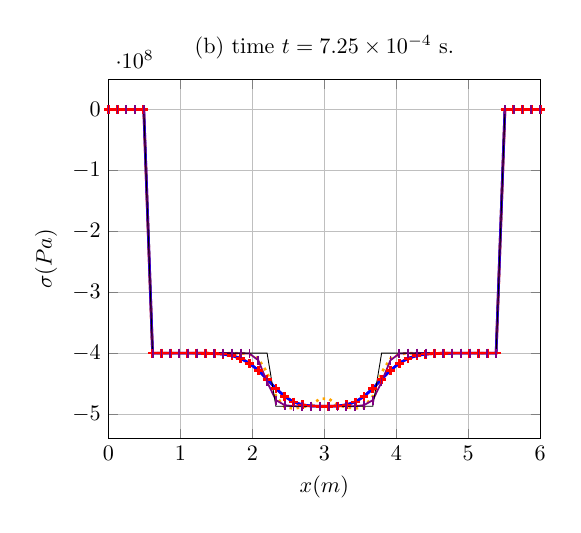
\begin{tikzpicture}[scale=0.8]
\begin{axis}[xlabel=$x (m)$,ylabel=$\sigma (Pa)$,ymajorgrids=true,xmajorgrids=true,legend pos=outer north east,title={(b) time $t = 7.25\times 10^{-4} $ s.},xmin=0.,xmax=6.]
\addplot[Red,very thick,mark=+,solid] coordinates {(0.0,-0.016398596440346053) (0.12244897959183673,-0.06425322857955201) (0.24489795918367346,-0.7380674881804443) (0.36734693877551017,-2.12047390173559) (0.4897959183673469,-28.76271861558054) (0.6122448979591837,-400000015.4159754) (0.7346938775510203,-400000102.7573024) (0.8571428571428571,-400000598.1932516) (0.9795918367346939,-400003055.79803795) (1.1020408163265305,-400013747.0436081) (1.2244897959183674,-400054602.7199052) (1.346938775510204,-400191823.2382515) (1.4693877551020407,-400596672.6802674) (1.5918367346938775,-401644186.51493835) (1.7142857142857142,-404014374.4754996) (1.836734693877551,-408684632.25449073) (1.9591836734693877,-416652037.9726774) (2.0816326530612246,-428329061.0045163) (2.204081632653061,-442879954.5361007) (2.326530612244898,-458084443.80872595) (2.4489795918367347,-471157539.9020842) (2.571428571428571,-480164339.19475454) (2.693877551020408,-484944715.5259052) (2.816326530612245,-486779650.5319825) (2.9387755102040813,-487233015.60471344) (3.061224489795918,-487233015.60471344) (3.183673469387755,-486779650.5319825) (3.306122448979592,-484944715.5259052) (3.4285714285714284,-480164339.19475454) (3.5510204081632653,-471157539.9020842) (3.673469387755102,-458084443.80872613) (3.7959183673469385,-442879954.5361007) (3.9183673469387754,-428329061.0045163) (4.040816326530612,-416652037.9726776) (4.163265306122449,-408684632.2544908) (4.285714285714286,-404014374.4754996) (4.408163265306122,-401644186.5149382) (4.530612244897959,-400596672.68026733) (4.653061224489796,-400191823.2382513) (4.775510204081632,-400054602.7199051) (4.8979591836734695,-400013747.04360807) (5.020408163265306,-400003055.79803795) (5.142857142857142,-400000598.19325155) (5.26530612244898,-400000102.75730234) (5.387755102040816,-400000015.4159754) (5.5102040816326525,-28.762718512303003) (5.63265306122449,-2.1204742438100417) (5.755102040816326,-0.7380675867576459) (5.877551020408163,-0.06425320166977637) (6.0,-0.01639854380134023) };
\addplot[Orange,very thick,mark=none,dotted] coordinates {(0.0011999999999999927,0.0) (0.12359999999999997,2.8345154836222343e-06) (0.24599999999999994,0.0) (0.36839999999999995,-5.6690309672444694e-06) (0.4907999999999999,5.563100179036459e-06) (0.6131999999999999,-400000000.00000036) (0.7355999999999999,-400000000.00000095) (0.858,-400000000.0000158) (0.9803999999999998,-400000000.000588) (1.1027999999999998,-400000000.0183558) (1.2251999999999996,-400000000.47669524) (1.3475999999999997,-400000010.242256) (1.4699999999999998,-400000180.58382314) (1.5923999999999996,-400002583.79875094) (1.7147999999999997,-400029558.11391515) (1.8371999999999995,-400265019.7421873) (1.9595999999999996,-401812442.4208182) (2.0819999999999994,-409100274.22059995) (2.2043999999999997,-431724216.84982246) (2.3267999999999995,-470516941.3021229) (2.4491999999999994,-488918339.55243546) (2.5715999999999997,-490903509.0666595) (2.6939999999999995,-488910392.160918) (2.8163999999999993,-485129466.2005724) (2.9387999999999996,-474875832.26573056) (3.0611999999999995,-474875832.26572955) (3.1835999999999993,-485129466.20057756) (3.305999999999999,-488910392.1609156) (3.4283999999999994,-490903509.0666595) (3.5507999999999993,-488918339.5524351) (3.673199999999999,-470516941.30212307) (3.7955999999999994,-431724216.8498228) (3.9179999999999993,-409100274.22060007) (4.040399999999999,-401812442.42081815) (4.1628,-400265019.742187) (4.2852,-400029558.11391526) (4.4076,-400002583.79875064) (4.53,-400000180.5838233) (4.6524,-400000010.242256) (4.7748,-400000000.47669554) (4.8972,-400000000.01835567) (5.0196,-400000000.00058854) (5.142,-400000000.00001574) (5.2644,-400000000.0000007) (5.3868,-400000000.0) (5.5092,-2.660415564296186e-06) (5.6316,-2.493917513477148e-06) (5.754,-2.7171818926536604e-06) (5.8764,3.405979701450893e-07) (5.9988,-2.8345154836222373e-06) };
\addplot[Blue,very thick,mark=none,solid] coordinates {(0.0011999999999999927,-0.00357849008468239) (0.12359999999999997,-0.06440079814818947) (0.24599999999999994,-0.21143910174666652) (0.36839999999999995,-2.1204748738318564) (0.4907999999999999,-3.2714037895202637) (0.6131999999999999,-400000015.4159753) (0.7355999999999999,-400000102.75730234) (0.858,-400000598.1932516) (0.9803999999999998,-400003055.79803795) (1.1027999999999998,-400013747.04360807) (1.2251999999999996,-400054602.7199051) (1.3475999999999997,-400191823.2382513) (1.4699999999999998,-400596672.68026733) (1.5923999999999996,-401644186.5149383) (1.7147999999999997,-404014374.47549963) (1.8371999999999995,-408684632.25449085) (1.9595999999999996,-416652037.9726776) (2.0819999999999994,-428329061.00451636) (2.2043999999999997,-442879954.5361008) (2.3267999999999995,-458084443.80872625) (2.4491999999999994,-471157539.9020842) (2.5715999999999997,-480164339.1947546) (2.6939999999999995,-484944715.52590525) (2.8163999999999993,-486779650.5319826) (2.9387999999999996,-487233015.60471344) (3.0611999999999995,-487233015.60471344) (3.1835999999999993,-486779650.5319826) (3.305999999999999,-484944715.52590525) (3.4283999999999994,-480164339.1947546) (3.5507999999999993,-471157539.9020842) (3.673199999999999,-458084443.80872625) (3.7955999999999994,-442879954.5361008) (3.9179999999999993,-428329061.00451636) (4.040399999999999,-416652037.9726776) (4.1628,-408684632.25449085) (4.2852,-404014374.47549963) (4.4076,-401644186.5149383) (4.53,-400596672.68026733) (4.6524,-400191823.2382513) (4.7748,-400054602.7199051) (4.8972,-400013747.04360807) (5.0196,-400003055.79803795) (5.142,-400000598.1932516) (5.2644,-400000102.75730234) (5.3868,-400000015.4159753) (5.5092,-3.2714037895202637) (5.6316,-2.1204748738318564) (5.754,-0.21143910174666652) (5.8764,-0.06440079814818947) (5.9988,-0.00357849008468239) };
\addplot[Purple,thick,mark=|,solid] coordinates {(0.0011999999999999927,1.6543612251060583e-24) (0.12359999999999997,1.6543612251060553e-23) (0.24599999999999994,2.452440800103604e-08) (0.36839999999999995,-3.508023677435457e-08) (0.4907999999999999,-5.960464477539063e-08) (0.6131999999999999,-400000000.0) (0.7355999999999999,-400000000.0) (0.858,-400000000.0000003) (0.9803999999999998,-400000000.0000133) (1.1027999999999998,-400000000.0004144) (1.2251999999999996,-400000000.0115142) (1.3475999999999997,-400000000.2871339) (1.4699999999999998,-400000006.46675307) (1.5923999999999996,-400000132.73197645) (1.7147999999999997,-400002510.7191475) (1.8371999999999995,-400043970.06492174) (1.9595999999999996,-400741455.361692) (2.0819999999999994,-411776022.67189264) (2.2043999999999997,-447347518.96724993) (2.3267999999999995,-477210124.05958325) (2.4491999999999994,-485453941.80645174) (2.5715999999999997,-487021615.6680456) (2.6939999999999995,-487258956.9032909) (2.8163999999999993,-487285223.6098061) (2.9387999999999996,-487287092.0986835) (3.0611999999999995,-487287092.0986835) (3.1835999999999993,-487285223.6098061) (3.305999999999999,-487258956.9032909) (3.4283999999999994,-487021615.6680456) (3.5507999999999993,-485453941.80645174) (3.673199999999999,-477210124.05958325) (3.7955999999999994,-447347518.96724993) (3.9179999999999993,-411776022.67189264) (4.040399999999999,-400741455.361692) (4.1628,-400043970.06492174) (4.2852,-400002510.71914756) (4.4076,-400000132.73197645) (4.53,-400000006.466753) (4.6524,-400000000.287134) (4.7748,-400000000.01151425) (4.8972,-400000000.0004144) (5.0196,-400000000.0000133) (5.142,-400000000.0000003) (5.2644,-400000000.0) (5.3868,-400000000.0) (5.5092,-5.960464477539063e-08) (5.6316,-3.508023677435457e-08) (5.754,2.452440800103604e-08) (5.8764,1.6543612251060553e-23) (5.9988,1.6543612251060583e-24) };
\addplot[black,thin,mark=none,solid] coordinates {(0.0,-0.0) (0.12244897959183673,-0.0) (0.24489795918367346,-0.0) (0.36734693877551017,-0.0) (0.4897959183673469,-0.0) (0.6122448979591837,-400000000.0) (0.7346938775510203,-400000000.0) (0.8571428571428571,-400000000.0) (0.9795918367346939,-400000000.0) (1.1020408163265305,-400000000.0) (1.2244897959183674,-400000000.0) (1.346938775510204,-400000000.0) (1.4693877551020407,-400000000.0) (1.5918367346938775,-400000000.0) (1.7142857142857142,-400000000.0) (1.836734693877551,-400000000.0) (1.9591836734693877,-400000000.0) (2.0816326530612246,-400000000.0) (2.204081632653061,-400000000.0) (2.326530612244898,-487287156.09439695) (2.4489795918367347,-487287156.09439695) (2.571428571428571,-487287156.09439695) (2.693877551020408,-487287156.09439695) (2.816326530612245,-487287156.09439695) (2.9387755102040813,-487287156.09439695) (3.061224489795918,-487287156.09439695) (3.183673469387755,-487287156.09439695) (3.306122448979592,-487287156.09439695) (3.4285714285714284,-487287156.09439695) (3.5510204081632653,-487287156.09439695) (3.673469387755102,-487287156.09439695) (3.7959183673469385,-400000000.0) (3.9183673469387754,-400000000.0) (4.040816326530612,-400000000.0) (4.163265306122449,-400000000.0) (4.285714285714286,-400000000.0) (4.408163265306122,-400000000.0) (4.530612244897959,-400000000.0) (4.653061224489796,-400000000.0) (4.775510204081632,-400000000.0) (4.8979591836734695,-400000000.0) (5.020408163265306,-400000000.0) (5.142857142857142,-400000000.0) (5.26530612244898,-400000000.0) (5.387755102040816,-400000000.0) (5.5102040816326525,-0.0) (5.63265306122449,-0.0) (5.755102040816326,-0.0) (5.877551020408163,-0.0) (6.0,-0.0) };
%\legend{dgmpm,fem,fvm,fvm (SB),exact}
\end{axis}
\end{tikzpicture}
%%% Local Variables:
%%% mode: latex
%%% TeX-master: "../../mainManuscript"
%%% End:
}
  {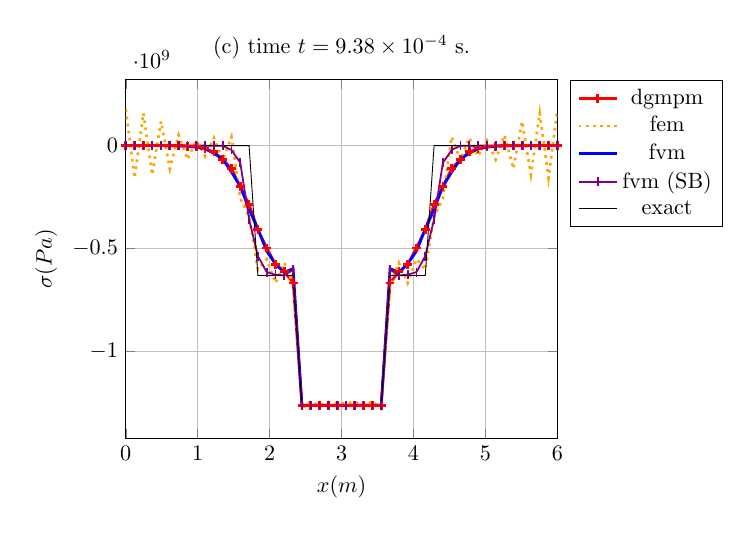
\begin{tikzpicture}[scale=0.8]
\begin{axis}[xlabel=$x (m)$,ylabel=$\sigma (Pa)$,ymajorgrids=true,xmajorgrids=true,legend pos=outer north east,title={(c) time $t = 9.38\times 10^{-4} $ s.},xmin=0.,xmax=6.]
\addplot[Red,very thick,mark=+,solid] coordinates {(0.0,-288.000337932026) (0.12244897959183673,-2340.8049612902105) (0.24489795918367346,-6717.6736351549625) (0.36734693877551017,-31436.18543893099) (0.4897959183673469,-82819.9714218378) (0.6122448979591837,-326370.9123286009) (0.7346938775510203,-787154.078435719) (0.8571428571428571,-2592039.5752673745) (0.9795918367346939,-5646941.091449857) (1.1020408163265305,-15363721.703146875) (1.2244897959183674,-29743749.6379236) (1.346938775510204,-65953645.19968581) (1.4693877551020407,-111309952.1584177) (1.5918367346938775,-198327314.77079153) (1.7142857142857142,-286130814.5665445) (1.836734693877551,-406728211.7590298) (1.9591836734693877,-496866659.9258773) (2.0816326530612246,-575814412.3291713) (2.204081632653061,-612581021.5556202) (2.326530612244898,-666589640.9783583) (2.4489795918367347,-1261004576.2605588) (2.571428571428571,-1261004576.2605588) (2.693877551020408,-1261004576.2605588) (2.816326530612245,-1261004576.2605593) (2.9387755102040813,-1261004576.2605593) (3.061224489795918,-1261004576.2605588) (3.183673469387755,-1261004576.2605584) (3.306122448979592,-1261004576.2605593) (3.4285714285714284,-1261004576.2605581) (3.5510204081632653,-1261004576.2605588) (3.673469387755102,-666589640.9783561) (3.7959183673469385,-612581021.5556188) (3.9183673469387754,-575814412.3291719) (4.040816326530612,-496866659.9258761) (4.163265306122449,-406728211.75903) (4.285714285714286,-286130814.5665426) (4.408163265306122,-198327314.77079123) (4.530612244897959,-111309952.15841806) (4.653061224489796,-65953645.19968575) (4.775510204081632,-29743749.637924016) (4.8979591836734695,-15363721.703146577) (5.020408163265306,-5646941.091449976) (5.142857142857142,-2592039.5752685666) (5.26530612244898,-787154.0784354806) (5.387755102040816,-326370.91232824326) (5.5102040816326525,-82819.97142159939) (5.63265306122449,-31436.185439646244) (5.755102040816326,-6717.673635229468) (5.877551020408163,-2340.804961979389) (6.0,-288.00033782143146) };
\addplot[Orange,very thick,mark=none,dotted] coordinates {(0.0011999999999999927,175010887.86141148) (0.12359999999999997,-157010320.72319484) (0.24599999999999994,157731015.99830914) (0.36839999999999995,-141347084.0250168) (0.4907999999999999,117914146.10742596) (0.6131999999999999,-112262666.61428112) (0.7355999999999999,51745557.76652613) (0.858,-67268258.78012908) (0.9803999999999998,25135893.71762538) (1.1027999999999998,-51161038.25586742) (1.2251999999999996,38244096.87732005) (1.3475999999999997,-71286114.06399637) (1.4699999999999998,42529781.300441384) (1.5923999999999996,-256057713.884533) (1.7147999999999997,-344993293.7306862) (1.8371999999999995,-602082756.2554108) (1.9595999999999996,-551416188.3408538) (2.0819999999999994,-667542863.5679615) (2.2043999999999997,-569236978.9147782) (2.3267999999999995,-673381420.6974866) (2.4491999999999994,-1276652083.3178082) (2.5715999999999997,-1242412632.5978575) (2.6939999999999995,-1262303877.9393654) (2.8163999999999993,-1245296647.9512377) (2.9387999999999996,-1251720925.4068818) (3.0611999999999995,-1251720925.406923) (3.1835999999999993,-1245296647.951198) (3.305999999999999,-1262303877.9393706) (3.4283999999999994,-1242412632.5978665) (3.5507999999999993,-1276652083.3177838) (3.673199999999999,-673381420.6975331) (3.7955999999999994,-569236978.9147345) (3.9179999999999993,-667542863.5679996) (4.040399999999999,-551416188.3408496) (4.1628,-602082756.2553713) (4.2852,-344993293.7307386) (4.4076,-256057713.88448328) (4.53,42529781.300438166) (4.6524,-71286114.06398582) (4.7748,38244096.877307296) (4.8972,-51161038.2558347) (5.0196,25135893.71758467) (5.142,-67268258.78007948) (5.2644,51745557.766474634) (5.3868,-112262666.6142239) (5.5092,117914146.10736191) (5.6316,-141347084.02495122) (5.754,157731015.9982485) (5.8764,-157010320.7231324) (5.9988,175010887.86135092) };
\addplot[Blue,very thick,mark=none,solid] coordinates {(0.0011999999999999927,-672.000788774134) (0.12359999999999997,-2317.190485430212) (0.24599999999999994,-11624.7450740413) (0.36839999999999995,-31435.028274873635) (0.4907999999999999,-131180.5918317446) (0.6131999999999999,-326370.86669091054) (0.7355999999999999,-1145540.9690250745) (0.858,-2592039.5738099255) (0.9803999999999998,-7576352.574992208) (1.1027999999999998,-15363721.703109615) (1.2251999999999996,-36933763.60530679) (1.3475999999999997,-65953645.19968625) (1.4699999999999998,-128588545.2855558) (1.5923999999999996,-198327314.77079248) (1.7147999999999997,-310077223.60174906) (1.8371999999999995,-406728211.759032) (1.9595999999999996,-512542911.78098124) (2.0819999999999994,-575814412.329173) (2.2043999999999997,-615644905.6578237) (2.3267999999999995,-597093014.0061195) (2.4491999999999994,-1261004576.2605588) (2.5715999999999997,-1261004576.2605586) (2.6939999999999995,-1261004576.2605588) (2.8163999999999993,-1261004576.2605584) (2.9387999999999996,-1261004576.2605588) (3.0611999999999995,-1261004576.2605586) (3.1835999999999993,-1261004576.2605586) (3.305999999999999,-1261004576.2605586) (3.4283999999999994,-1261004576.2605588) (3.5507999999999993,-1261004576.2605584) (3.673199999999999,-597093014.0061196) (3.7955999999999994,-615644905.6578233) (3.9179999999999993,-575814412.329173) (4.040399999999999,-512542911.78098106) (4.1628,-406728211.759032) (4.2852,-310077223.601749) (4.4076,-198327314.77079242) (4.53,-128588545.28555562) (4.6524,-65953645.199686386) (4.7748,-36933763.60530707) (4.8972,-15363721.703109678) (5.0196,-7576352.5749919815) (5.142,-2592039.5738102393) (5.2644,-1145540.9690254903) (5.3868,-326370.8666910869) (5.5092,-131180.5918318261) (5.6316,-31435.028275203294) (5.754,-11624.74507411075) (5.8764,-2317.1904855701214) (5.9988,-672.0007888251785) };
\addplot[Purple,thick,mark=|,solid] coordinates {(0.0011999999999999927,-2.2554342869669835e-07) (0.12359999999999997,-4.253451172600671e-07) (0.24599999999999994,-1.2920591556701192e-05) (0.36839999999999995,-5.986342632906781e-05) (0.4907999999999999,-0.0056401329400634255) (0.6131999999999999,-0.02444787812144389) (0.7355999999999999,-1.8760696294301331) (0.858,-7.9566149629172855) (0.9803999999999998,-503.4524595203254) (1.1027999999999998,-2086.1665527314763) (1.2251999999999996,-111480.01946610014) (1.3475999999999997,-452326.4024975486) (1.4699999999999998,-21130457.36149759) (1.5923999999999996,-83990511.6868726) (1.7147999999999997,-358373061.4587475) (1.8371999999999995,-536458450.92552686) (1.9595999999999996,-614366251.640357) (2.0819999999999994,-627343167.840607) (2.2043999999999997,-630228089.3811917) (2.3267999999999995,-602429197.2873981) (2.4491999999999994,-1261004576.2605584) (2.5715999999999997,-1261004576.2605586) (2.6939999999999995,-1261004576.2605581) (2.8163999999999993,-1261004576.2605586) (2.9387999999999996,-1261004576.2605584) (3.0611999999999995,-1261004576.2605586) (3.1835999999999993,-1261004576.2605584) (3.305999999999999,-1261004576.2605588) (3.4283999999999994,-1261004576.2605584) (3.5507999999999993,-1261004576.2605586) (3.673199999999999,-602429197.287398) (3.7955999999999994,-630228089.3811923) (3.9179999999999993,-627343167.8406069) (4.040399999999999,-614366251.6403568) (4.1628,-536458450.9255258) (4.2852,-358373061.45874953) (4.4076,-83990511.68687272) (4.53,-21130457.361496225) (4.6524,-452326.4024989642) (4.7748,-111480.01946637034) (4.8972,-2086.166552579263) (5.0196,-503.4524587330095) (5.142,-7.956613651988789) (5.2644,-1.8760695971344141) (5.3868,-0.024446596221118888) (5.5092,-0.005640085558921308) (5.6316,-6.008348006163438e-05) (5.754,-1.352714115819129e-05) (5.8764,-1.6124271861316672e-09) (5.9988,-1.7267558828412451e-07) };
\addplot[black,thin,mark=none,solid] coordinates {(0.0,-0.0) (0.12244897959183673,-0.0) (0.24489795918367346,-0.0) (0.36734693877551017,-0.0) (0.4897959183673469,-0.0) (0.6122448979591837,-0.0) (0.7346938775510203,-0.0) (0.8571428571428571,-0.0) (0.9795918367346939,-0.0) (1.1020408163265305,-0.0) (1.2244897959183674,-0.0) (1.346938775510204,-0.0) (1.4693877551020407,-0.0) (1.5918367346938775,-0.0) (1.7142857142857142,-0.0) (1.836734693877551,-630502288.1302795) (1.9591836734693877,-630502288.1302795) (2.0816326530612246,-630502288.1302795) (2.204081632653061,-630502288.1302795) (2.326530612244898,-630502288.1302795) (2.4489795918367347,-1261004576.260559) (2.571428571428571,-1261004576.260559) (2.693877551020408,-1261004576.260559) (2.816326530612245,-1261004576.260559) (2.9387755102040813,-1261004576.260559) (3.061224489795918,-1261004576.260559) (3.183673469387755,-1261004576.260559) (3.306122448979592,-1261004576.260559) (3.4285714285714284,-1261004576.260559) (3.5510204081632653,-1261004576.260559) (3.673469387755102,-630502288.1302795) (3.7959183673469385,-630502288.1302795) (3.9183673469387754,-630502288.1302795) (4.040816326530612,-630502288.1302795) (4.163265306122449,-630502288.1302795) (4.285714285714286,-0.0) (4.408163265306122,-0.0) (4.530612244897959,-0.0) (4.653061224489796,-0.0) (4.775510204081632,-0.0) (4.8979591836734695,-0.0) (5.020408163265306,-0.0) (5.142857142857142,-0.0) (5.26530612244898,-0.0) (5.387755102040816,-0.0) (5.5102040816326525,-0.0) (5.63265306122449,-0.0) (5.755102040816326,-0.0) (5.877551020408163,-0.0) (6.0,-0.0) };
\legend{dgmpm,fem,fvm,fvm (SB),exact}
\end{axis}
\end{tikzpicture}
%%% Local Variables:
%%% mode: latex
%%% TeX-master: "../../mainManuscript"
%%% End:
}
  \caption{elastic-plastic RP stress}
  \label{fig:stress_elastoplastic_RP}
\end{figure}
\begin{figure}[h!]
  \centering
  {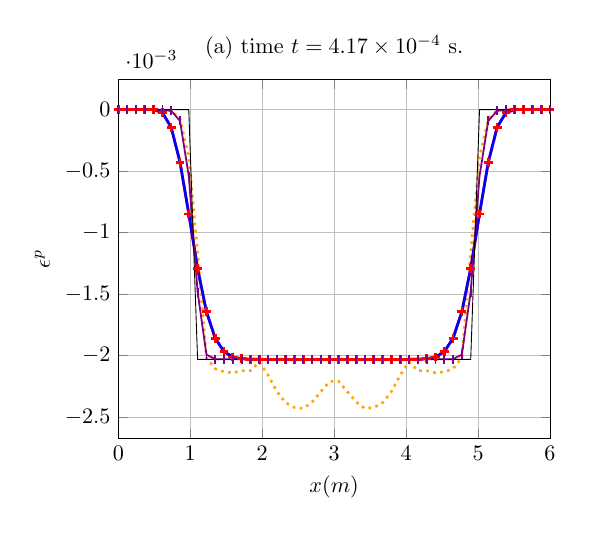
\begin{tikzpicture}[scale=0.8]
\begin{axis}[xlabel=$x (m)$,ylabel=$\epsilon^p$,ymajorgrids=true,xmajorgrids=true,legend pos=outer north east,title={(a) time $t = 4.17\times 10^{-4} $ s.},xmin=0.,xmax=6.]
\addplot[Red,very thick,mark=+,solid] coordinates {(0.0,0.0) (0.12244897959183673,0.0) (0.24489795918367346,0.0) (0.36734693877551017,0.0) (0.4897959183673469,0.0) (0.6122448979591837,-2.4267855226065594e-05) (0.7346938775510203,-0.00014452073597361284) (0.8571428571428571,-0.0004275642401009131) (0.9795918367346939,-0.0008483282066457896) (1.1020408163265305,-0.0012913872123487611) (1.2244897959183674,-0.001642660920094959) (1.346938775510204,-0.0018602413103573651) (1.4693877551020407,-0.0019680574666657586) (1.5918367346938775,-0.00201146561977191) (1.7142857142857142,-0.002025805454394895) (1.836734693877551,-0.0020297136017104972) (1.9591836734693877,-0.002030593864489664) (2.0816326530612246,-0.002030757436013639) (2.204081632653061,-0.0020307823755532774) (2.326530612244898,-0.002030785465084119) (2.4489795918367347,-0.0020307857712710334) (2.571428571428571,-0.00203078579497771) (2.693877551020408,-0.0020307857963597366) (2.816326530612245,-0.002030785796416807) (2.9387755102040813,-0.002030785796418294) (3.061224489795918,-0.002030785796418294) (3.183673469387755,-0.0020307857964168056) (3.306122448979592,-0.002030785796359739) (3.4285714285714284,-0.0020307857949777124) (3.5510204081632653,-0.002030785771271032) (3.673469387755102,-0.002030785465084119) (3.7959183673469385,-0.002030782375553277) (3.9183673469387754,-0.0020307574360136386) (4.040816326530612,-0.002030593864489664) (4.163265306122449,-0.0020297136017104964) (4.285714285714286,-0.0020258054543948927) (4.408163265306122,-0.002011465619771909) (4.530612244897959,-0.0019680574666657573) (4.653061224489796,-0.0018602413103573651) (4.775510204081632,-0.0016426609200949592) (4.8979591836734695,-0.001291387212348762) (5.020408163265306,-0.0008483282066457893) (5.142857142857142,-0.00042756424010091193) (5.26530612244898,-0.00014452073597361384) (5.387755102040816,-2.4267855226067292e-05) (5.5102040816326525,0.0) (5.63265306122449,0.0) (5.755102040816326,0.0) (5.877551020408163,0.0) (6.0,0.0) };
\addplot[Orange,very thick,mark=none,dotted] coordinates {(0.0011999999999999927,0.0) (0.12359999999999997,0.0) (0.24599999999999994,0.0) (0.36839999999999995,0.0) (0.4907999999999999,0.0) (0.6131999999999999,-3.6185144371068533e-07) (0.7355999999999999,-8.019549939201378e-06) (0.858,-7.545863055389513e-05) (0.9803999999999998,-0.00038823448768833166) (1.1027999999999998,-0.0011649510446652884) (1.2251999999999996,-0.0020167797859788647) (1.3475999999999997,-0.002107399619958115) (1.4699999999999998,-0.002131770374563102) (1.5923999999999996,-0.0021403574192086572) (1.7147999999999997,-0.0021224712498380525) (1.8371999999999995,-0.0021223153729543927) (1.9595999999999996,-0.002051517588290279) (2.0819999999999994,-0.00215869886386764) (2.2043999999999997,-0.00229323761080671) (2.3267999999999995,-0.002383730340592019) (2.4491999999999994,-0.002422023782426279) (2.5715999999999997,-0.0024301527006305407) (2.6939999999999995,-0.0023776240406298606) (2.8163999999999993,-0.0022924966391795762) (2.9387999999999996,-0.002209718054457858) (3.0611999999999995,-0.002209718054457853) (3.1835999999999993,-0.00229249663917957) (3.305999999999999,-0.002377624040629834) (3.4283999999999994,-0.0024301527006305133) (3.5507999999999993,-0.0024220237824262893) (3.673199999999999,-0.0023837303405920274) (3.7955999999999994,-0.0022932376108067225) (3.9179999999999993,-0.002158698863867652) (4.040399999999999,-0.0020515175882902612) (4.1628,-0.00212231537295439) (4.2852,-0.002122471249838043) (4.4076,-0.002140357419208655) (4.53,-0.0021317703745630944) (4.6524,-0.0021073996199581038) (4.7748,-0.002016779785978835) (4.8972,-0.0011649510446653149) (5.0196,-0.00038823448768831226) (5.142,-7.54586305539126e-05) (5.2644,-8.019549939178096e-06) (5.3868,-3.6185144371335306e-07) (5.5092,0.0) (5.6316,0.0) (5.754,0.0) (5.8764,0.0) (5.9988,0.0) };
\addplot[Blue,very thick,mark=none,solid] coordinates {(0.0011999999999999927,0.0) (0.12359999999999997,0.0) (0.24599999999999994,0.0) (0.36839999999999995,0.0) (0.4907999999999999,0.0) (0.6131999999999999,-2.4267855226066533e-05) (0.7355999999999999,-0.00014452073597361162) (0.858,-0.0004275642401009113) (0.9803999999999998,-0.0008483282066457879) (1.1027999999999998,-0.0012913872123487594) (1.2251999999999996,-0.0016426609200949575) (1.3475999999999997,-0.0018602413103573636) (1.4699999999999998,-0.0019680574666657573) (1.5923999999999996,-0.002011465619771908) (1.7147999999999997,-0.002025805454394894) (1.8371999999999995,-0.0020297136017104955) (1.9595999999999996,-0.0020305938644896646) (2.0819999999999994,-0.002030757436013637) (2.2043999999999997,-0.002030782375553278) (2.3267999999999995,-0.002030785465084118) (2.4491999999999994,-0.0020307857712710316) (2.5715999999999997,-0.002030785794977712) (2.6939999999999995,-0.002030785796359737) (2.8163999999999993,-0.002030785796416805) (2.9387999999999996,-0.0020307857964182922) (3.0611999999999995,-0.0020307857964182935) (3.1835999999999993,-0.002030785796416805) (3.305999999999999,-0.002030785796359737) (3.4283999999999994,-0.002030785794977712) (3.5507999999999993,-0.0020307857712710316) (3.673199999999999,-0.0020307854650841186) (3.7955999999999994,-0.002030782375553278) (3.9179999999999993,-0.002030757436013637) (4.040399999999999,-0.0020305938644896646) (4.1628,-0.0020297136017104955) (4.2852,-0.002025805454394893) (4.4076,-0.002011465619771907) (4.53,-0.0019680574666657573) (4.6524,-0.0018602413103573636) (4.7748,-0.0016426609200949566) (4.8972,-0.0012913872123487594) (5.0196,-0.0008483282066457876) (5.142,-0.0004275642401009109) (5.2644,-0.00014452073597361162) (5.3868,-2.4267855226066533e-05) (5.5092,0.0) (5.6316,0.0) (5.754,0.0) (5.8764,0.0) (5.9988,0.0) };
\addplot[Purple,thick,mark=|,solid] coordinates {(0.0011999999999999927,0.0) (0.12359999999999997,0.0) (0.24599999999999994,0.0) (0.36839999999999995,0.0) (0.4907999999999999,0.0) (0.6131999999999999,-5.394021759754931e-07) (0.7355999999999999,-1.010771354391672e-05) (0.858,-9.168096769918878e-05) (0.9803999999999998,-0.0005435535234499527) (1.1027999999999998,-0.0014841083655069223) (1.2251999999999996,-0.001991887176242578) (1.3475999999999997,-0.002028854598935097) (1.4699999999999998,-0.0020307027185062754) (1.5923999999999996,-0.002030782602337539) (1.7147999999999997,-0.0020307856903745234) (1.8371999999999995,-0.002030785793411752) (1.9595999999999996,-0.002030785796346042) (2.0819999999999994,-0.002030785796416862) (2.2043999999999997,-0.002030785796418289) (2.3267999999999995,-0.0020307857964183135) (2.4491999999999994,-0.0020307857964183135) (2.5715999999999997,-0.0020307857964183135) (2.6939999999999995,-0.0020307857964183135) (2.8163999999999993,-0.0020307857964183135) (2.9387999999999996,-0.0020307857964183135) (3.0611999999999995,-0.0020307857964183135) (3.1835999999999993,-0.0020307857964183135) (3.305999999999999,-0.0020307857964183126) (3.4283999999999994,-0.0020307857964183135) (3.5507999999999993,-0.0020307857964183126) (3.673199999999999,-0.0020307857964183126) (3.7955999999999994,-0.002030785796418291) (3.9179999999999993,-0.0020307857964168632) (4.040399999999999,-0.0020307857963460427) (4.1628,-0.0020307857934117523) (4.2852,-0.002030785690374525) (4.4076,-0.0020307826023375384) (4.53,-0.0020307027185062733) (4.6524,-0.002028854598935106) (4.7748,-0.0019918871762425686) (4.8972,-0.0014841083655069208) (5.0196,-0.0005435535234499549) (5.142,-9.168096769918878e-05) (5.2644,-1.010771354391672e-05) (5.3868,-5.394021759754931e-07) (5.5092,0.0) (5.6316,0.0) (5.754,0.0) (5.8764,0.0) (5.9988,0.0) };
\addplot[black,thin,mark=none,solid] coordinates {(0.0,-0.0) (0.12244897959183673,-0.0) (0.24489795918367346,-0.0) (0.36734693877551017,-0.0) (0.4897959183673469,-0.0) (0.6122448979591837,-0.0) (0.7346938775510203,-0.0) (0.8571428571428571,-0.0) (0.9795918367346939,-0.0) (1.1020408163265305,-0.002030785796418313) (1.2244897959183674,-0.002030785796418313) (1.346938775510204,-0.002030785796418313) (1.4693877551020407,-0.002030785796418313) (1.5918367346938775,-0.002030785796418313) (1.7142857142857142,-0.002030785796418313) (1.836734693877551,-0.002030785796418313) (1.9591836734693877,-0.002030785796418313) (2.0816326530612246,-0.002030785796418313) (2.204081632653061,-0.002030785796418313) (2.326530612244898,-0.002030785796418313) (2.4489795918367347,-0.002030785796418313) (2.571428571428571,-0.002030785796418313) (2.693877551020408,-0.002030785796418313) (2.816326530612245,-0.002030785796418313) (2.9387755102040813,-0.002030785796418313) (3.061224489795918,-0.002030785796418313) (3.183673469387755,-0.002030785796418313) (3.306122448979592,-0.002030785796418313) (3.4285714285714284,-0.002030785796418313) (3.5510204081632653,-0.002030785796418313) (3.673469387755102,-0.002030785796418313) (3.7959183673469385,-0.002030785796418313) (3.9183673469387754,-0.002030785796418313) (4.040816326530612,-0.002030785796418313) (4.163265306122449,-0.002030785796418313) (4.285714285714286,-0.002030785796418313) (4.408163265306122,-0.002030785796418313) (4.530612244897959,-0.002030785796418313) (4.653061224489796,-0.002030785796418313) (4.775510204081632,-0.002030785796418313) (4.8979591836734695,-0.002030785796418313) (5.020408163265306,-0.0) (5.142857142857142,-0.0) (5.26530612244898,-0.0) (5.387755102040816,-0.0) (5.5102040816326525,-0.0) (5.63265306122449,-0.0) (5.755102040816326,-0.0) (5.877551020408163,-0.0) (6.0,-0.0) };
%\legend{dgmpm,fem,fvm,fvm (SB),exact}
\end{axis}
\end{tikzpicture}
%%% Local Variables:
%%% mode: latex
%%% TeX-master: "../../mainManuscript"
%%% End:
}
  {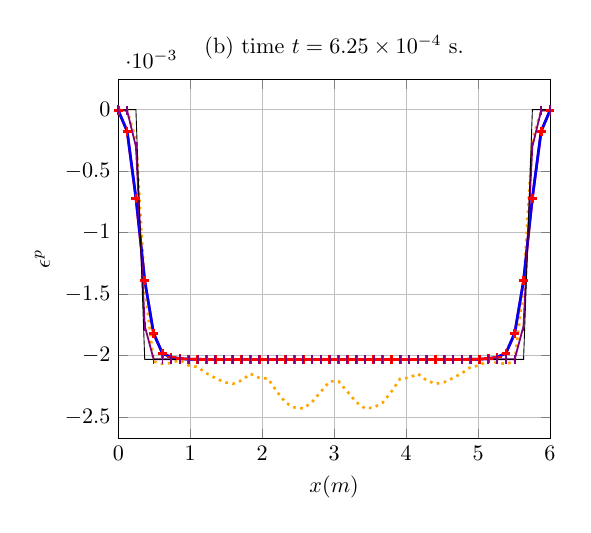
\begin{tikzpicture}[scale=0.8]
\begin{axis}[xlabel=$x (m)$,ylabel=$\epsilon^p$,ymajorgrids=true,xmajorgrids=true,legend pos=outer north east,title={(b) time $t = 6.25\times 10^{-4} $ s.},xmin=0.,xmax=6.]
\addplot[Red,very thick,mark=+,solid] coordinates {(0.0,-8.02367288935203e-06) (0.12244897959183673,-0.00017614426387335805) (0.24489795918367346,-0.0007207542691858686) (0.36734693877551017,-0.0013919930410856215) (0.4897959183673469,-0.001818355598439618) (0.6122448979591837,-0.001981300761387861) (0.7346938775510203,-0.0020125975551096974) (0.8571428571428571,-0.002024874952136019) (0.9795918367346939,-0.0020290867696967987) (1.1020408163265305,-0.002030353909504423) (1.2244897959183674,-0.0020306887880741907) (1.346938775510204,-0.0020307665725143873) (1.4693877551020407,-0.0020307824435747243) (1.5918367346938775,-0.0020307852835259937) (1.7142857142857142,-0.0020307857279245408) (1.836734693877551,-0.0020307857884822454) (1.9591836734693877,-0.00203078579562695) (2.0816326530612246,-0.002030785796351117) (2.204081632653061,-0.0020307857964135248) (2.326530612244898,-0.002030785796418031) (2.4489795918367347,-0.002030785796418302) (2.571428571428571,-0.0020307857964183135) (2.693877551020408,-0.002030785796418313) (2.816326530612245,-0.002030785796418313) (2.9387755102040813,-0.002030785796418314) (3.061224489795918,-0.0020307857964183135) (3.183673469387755,-0.0020307857964183135) (3.306122448979592,-0.0020307857964183126) (3.4285714285714284,-0.0020307857964183113) (3.5510204081632653,-0.0020307857964183005) (3.673469387755102,-0.002030785796418031) (3.7959183673469385,-0.0020307857964135217) (3.9183673469387754,-0.0020307857963511138) (4.040816326530612,-0.002030785795626948) (4.163265306122449,-0.0020307857884822433) (4.285714285714286,-0.0020307857279245403) (4.408163265306122,-0.0020307852835259915) (4.530612244897959,-0.0020307824435747226) (4.653061224489796,-0.0020307665725143842) (4.775510204081632,-0.002030688788074188) (4.8979591836734695,-0.0020303539095044196) (5.020408163265306,-0.0020290867696967953) (5.142857142857142,-0.0020248749521360144) (5.26530612244898,-0.0020125975551096966) (5.387755102040816,-0.0019813007613878565) (5.5102040816326525,-0.0018183555984396154) (5.63265306122449,-0.0013919930410856195) (5.755102040816326,-0.0007207542691858678) (5.877551020408163,-0.0001761442638733595) (6.0,-8.023672889353243e-06) };
\addplot[Orange,very thick,mark=none,dotted] coordinates {(0.0011999999999999927,-3.955614396475477e-08) (0.12359999999999997,-9.316948262183543e-06) (0.24599999999999994,-0.00024388789370993148) (0.36839999999999995,-0.001442592108388968) (0.4907999999999999,-0.00204828198640817) (0.6131999999999999,-0.002067557310378223) (0.7355999999999999,-0.0020594157964176534) (0.858,-0.0020372674628823476) (0.9803999999999998,-0.0020807928937422093) (1.1027999999999998,-0.0020931249622338447) (1.2251999999999996,-0.0021438341556582357) (1.3475999999999997,-0.0021820311184349702) (1.4699999999999998,-0.002216170966229309) (1.5923999999999996,-0.002229918265686059) (1.7147999999999997,-0.002201581328157663) (1.8371999999999995,-0.0021483028099073733) (1.9595999999999996,-0.002180462898277691) (2.0819999999999994,-0.0021876731020669623) (2.2043999999999997,-0.00229323761080671) (2.3267999999999995,-0.002383730340592019) (2.4491999999999994,-0.002422023782426279) (2.5715999999999997,-0.0024301527006305407) (2.6939999999999995,-0.0023776240406298606) (2.8163999999999993,-0.0022924966391795762) (2.9387999999999996,-0.002209718054457858) (3.0611999999999995,-0.002209718054457853) (3.1835999999999993,-0.00229249663917957) (3.305999999999999,-0.002377624040629834) (3.4283999999999994,-0.0024301527006305133) (3.5507999999999993,-0.0024220237824262893) (3.673199999999999,-0.0023837303405920274) (3.7955999999999994,-0.0022932376108067225) (3.9179999999999993,-0.002187673102066998) (4.040399999999999,-0.0021804628982777176) (4.1628,-0.002148302809907372) (4.2852,-0.00220158132815765) (4.4076,-0.0022299182656860483) (4.53,-0.0022161709662292563) (4.6524,-0.0021820311184349156) (4.7748,-0.002143834155658191) (4.8972,-0.0020931249622338105) (5.0196,-0.002080792893742207) (5.142,-0.002037267462882373) (5.2644,-0.002059415796417687) (5.3868,-0.0020675573103782394) (5.5092,-0.0020482819864081916) (5.6316,-0.0014425921083889624) (5.754,-0.00024388789370993877) (5.8764,-9.316948262168749e-06) (5.9988,-3.955614396669495e-08) };
\addplot[Blue,very thick,mark=none,solid] coordinates {(0.0011999999999999927,-8.023672889352762e-06) (0.12359999999999997,-0.00017614426387335818) (0.24599999999999994,-0.0007207542691858663) (0.36839999999999995,-0.0013919930410856193) (0.4907999999999999,-0.0018183555984396156) (0.6131999999999999,-0.0019813007613878556) (0.7355999999999999,-0.0020125975551096944) (0.858,-0.0020248749521360153) (0.9803999999999998,-0.002029086769696795) (1.1027999999999998,-0.0020303539095044188) (1.2251999999999996,-0.0020306887880741876) (1.3475999999999997,-0.0020307665725143834) (1.4699999999999998,-0.0020307824435747226) (1.5923999999999996,-0.0020307852835259902) (1.7147999999999997,-0.002030785727924537) (1.8371999999999995,-0.002030785788482242) (1.9595999999999996,-0.002030785795626947) (2.0819999999999994,-0.002030785796351112) (2.2043999999999997,-0.0020307857964135196) (2.3267999999999995,-0.002030785796418031) (2.4491999999999994,-0.0020307857964183005) (2.5715999999999997,-0.0020307857964183126) (2.6939999999999995,-0.0020307857964183143) (2.8163999999999993,-0.0020307857964183143) (2.9387999999999996,-0.0020307857964183143) (3.0611999999999995,-0.0020307857964183135) (3.1835999999999993,-0.0020307857964183135) (3.305999999999999,-0.0020307857964183135) (3.4283999999999994,-0.0020307857964183135) (3.5507999999999993,-0.0020307857964183005) (3.673199999999999,-0.0020307857964180303) (3.7955999999999994,-0.002030785796413521) (3.9179999999999993,-0.0020307857963511138) (4.040399999999999,-0.002030785795626947) (4.1628,-0.002030785788482243) (4.2852,-0.0020307857279245373) (4.4076,-0.0020307852835259902) (4.53,-0.0020307824435747213) (4.6524,-0.0020307665725143834) (4.7748,-0.0020306887880741867) (4.8972,-0.0020303539095044188) (5.0196,-0.002029086769696795) (5.142,-0.0020248749521360153) (5.2644,-0.0020125975551096944) (5.3868,-0.001981300761387855) (5.5092,-0.001818355598439614) (5.6316,-0.0013919930410856186) (5.754,-0.0007207542691858663) (5.8764,-0.0001761442638733578) (5.9988,-8.023672889352762e-06) };
\addplot[Purple,thick,mark=|,solid] coordinates {(0.0011999999999999927,-5.896527565960431e-08) (0.12359999999999997,-1.0175215434139024e-05) (0.24599999999999994,-0.00030290594091646547) (0.36839999999999995,-0.0017602606272338914) (0.4907999999999999,-0.002029328897607904) (0.6131999999999999,-0.0020307790770812324) (0.7355999999999999,-0.0020307854952318397) (0.858,-0.00203078578407098) (0.9803999999999998,-0.0020307857959587752) (1.1027999999999998,-0.002030785796402892) (1.2251999999999996,-0.002030785796417849) (1.3475999999999997,-0.0020307857964183013) (1.4699999999999998,-0.0020307857964183135) (1.5923999999999996,-0.0020307857964183126) (1.7147999999999997,-0.0020307857964183135) (1.8371999999999995,-0.0020307857964183135) (1.9595999999999996,-0.0020307857964183135) (2.0819999999999994,-0.0020307857964183126) (2.2043999999999997,-0.0020307857964183135) (2.3267999999999995,-0.0020307857964183135) (2.4491999999999994,-0.0020307857964183135) (2.5715999999999997,-0.0020307857964183135) (2.6939999999999995,-0.0020307857964183135) (2.8163999999999993,-0.0020307857964183135) (2.9387999999999996,-0.0020307857964183135) (3.0611999999999995,-0.0020307857964183135) (3.1835999999999993,-0.0020307857964183135) (3.305999999999999,-0.0020307857964183135) (3.4283999999999994,-0.0020307857964183135) (3.5507999999999993,-0.0020307857964183135) (3.673199999999999,-0.0020307857964183135) (3.7955999999999994,-0.0020307857964183126) (3.9179999999999993,-0.0020307857964183135) (4.040399999999999,-0.0020307857964183135) (4.1628,-0.0020307857964183126) (4.2852,-0.0020307857964183117) (4.4076,-0.0020307857964183117) (4.53,-0.0020307857964183117) (4.6524,-0.0020307857964182996) (4.7748,-0.0020307857964178473) (4.8972,-0.002030785796402895) (5.0196,-0.002030785795958776) (5.142,-0.002030785784070983) (5.2644,-0.002030785495231843) (5.3868,-0.0020307790770812315) (5.5092,-0.0020293288976078977) (5.6316,-0.0017602606272338914) (5.754,-0.0003029059409164685) (5.8764,-1.0175215434139024e-05) (5.9988,-5.896527565960431e-08) };
\addplot[black,thin,mark=none,solid] coordinates {(0.0,-0.0) (0.12244897959183673,-0.0) (0.24489795918367346,-0.0) (0.36734693877551017,-0.002030785796418313) (0.4897959183673469,-0.002030785796418313) (0.6122448979591837,-0.002030785796418313) (0.7346938775510203,-0.002030785796418313) (0.8571428571428571,-0.002030785796418313) (0.9795918367346939,-0.002030785796418313) (1.1020408163265305,-0.002030785796418313) (1.2244897959183674,-0.002030785796418313) (1.346938775510204,-0.002030785796418313) (1.4693877551020407,-0.002030785796418313) (1.5918367346938775,-0.002030785796418313) (1.7142857142857142,-0.002030785796418313) (1.836734693877551,-0.002030785796418313) (1.9591836734693877,-0.002030785796418313) (2.0816326530612246,-0.002030785796418313) (2.204081632653061,-0.002030785796418313) (2.326530612244898,-0.002030785796418313) (2.4489795918367347,-0.002030785796418313) (2.571428571428571,-0.002030785796418313) (2.693877551020408,-0.002030785796418313) (2.816326530612245,-0.002030785796418313) (2.9387755102040813,-0.002030785796418313) (3.061224489795918,-0.002030785796418313) (3.183673469387755,-0.002030785796418313) (3.306122448979592,-0.002030785796418313) (3.4285714285714284,-0.002030785796418313) (3.5510204081632653,-0.002030785796418313) (3.673469387755102,-0.002030785796418313) (3.7959183673469385,-0.002030785796418313) (3.9183673469387754,-0.002030785796418313) (4.040816326530612,-0.002030785796418313) (4.163265306122449,-0.002030785796418313) (4.285714285714286,-0.002030785796418313) (4.408163265306122,-0.002030785796418313) (4.530612244897959,-0.002030785796418313) (4.653061224489796,-0.002030785796418313) (4.775510204081632,-0.002030785796418313) (4.8979591836734695,-0.002030785796418313) (5.020408163265306,-0.002030785796418313) (5.142857142857142,-0.002030785796418313) (5.26530612244898,-0.002030785796418313) (5.387755102040816,-0.002030785796418313) (5.5102040816326525,-0.002030785796418313) (5.63265306122449,-0.002030785796418313) (5.755102040816326,-0.0) (5.877551020408163,-0.0) (6.0,-0.0) };
%\legend{dgmpm,fem,fvm,fvm (SB),exact}
\end{axis}
\end{tikzpicture}
%%% Local Variables:
%%% mode: latex
%%% TeX-master: "../../mainManuscript"
%%% End:
}
  {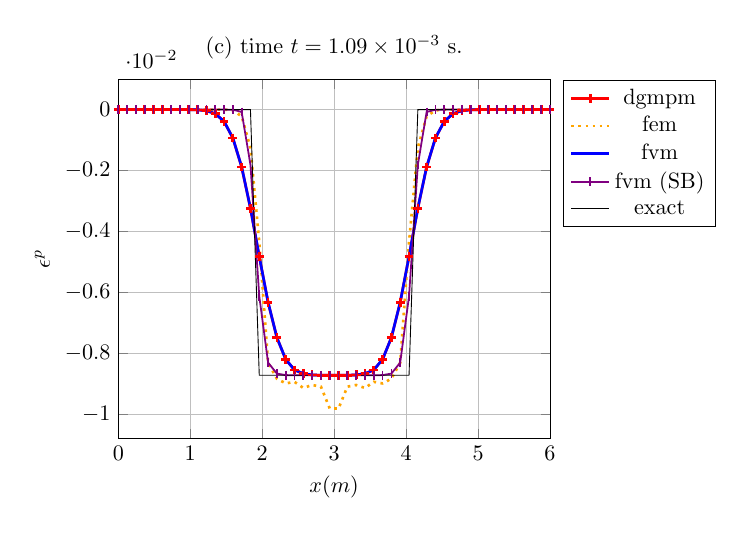
\begin{tikzpicture}[scale=0.8]
\begin{axis}[xlabel=$x (m)$,ylabel=$\epsilon^p$,ymajorgrids=true,xmajorgrids=true,legend pos=outer north east,title={(c) time $t = 1.09\times 10^{-3} $ s.},xmin=0.,xmax=6.]
\addplot[Red,very thick,mark=+,solid] coordinates {(0.0,-5.676632835751488e-19) (0.12244897959183673,-2.3898624238513766e-16) (0.24489795918367346,-3.735990751357306e-14) (0.36734693877551017,-2.3089144911084856e-12) (0.4897959183673469,-7.596762237094698e-11) (0.6122448979591837,-1.5415975357804979e-09) (0.7346938775510203,-2.1087029002110162e-08) (0.8571428571428571,-2.0628580472526095e-07) (0.9795918367346939,-1.5051975779320511e-06) (1.1020408163265305,-8.452232526292688e-06) (1.2244897959183674,-3.741900938747327e-05) (1.346938775510204,-0.00013315210803806102) (1.4693877551020407,-0.00038701776930482674) (1.5918367346938775,-0.0009319386970470464) (1.7142857142857142,-0.0018842066770200564) (1.836734693877551,-0.0032431409441831516) (1.9591836734693877,-0.004827293901207316) (2.0816326530612246,-0.00633202118341673) (2.204081632653061,-0.007489880430691718) (2.326530612244898,-0.008204526972019307) (2.4489795918367347,-0.008552921390073501) (2.571428571428571,-0.008674876019514461) (2.693877551020408,-0.008716486656783273) (2.816326530612245,-0.008726887116624966) (2.9387755102040813,-0.008728580772745199) (3.061224489795918,-0.008728580772745199) (3.183673469387755,-0.008726887116624966) (3.306122448979592,-0.00871648665678328) (3.4285714285714284,-0.008674876019514466) (3.5510204081632653,-0.008552921390073511) (3.673469387755102,-0.008204526972019318) (3.7959183673469385,-0.007489880430691721) (3.9183673469387754,-0.00633202118341673) (4.040816326530612,-0.0048272939012073204) (4.163265306122449,-0.0032431409441831525) (4.285714285714286,-0.001884206677020053) (4.408163265306122,-0.0009319386970470392) (4.530612244897959,-0.0003870177693048181) (4.653061224489796,-0.0001331521080380519) (4.775510204081632,-3.7419009387462476e-05) (4.8979591836734695,-8.452232526284741e-06) (5.020408163265306,-1.5051975779246716e-06) (5.142857142857142,-2.0628580471617835e-07) (5.26530612244898,-2.1087028991608393e-08) (5.387755102040816,-1.5415975312391917e-09) (5.5102040816326525,-7.596762123562041e-11) (5.63265306122449,-2.308913923445202e-12) (5.755102040816326,-3.7358772187005907e-14) (5.877551020408163,-2.4097306387765065e-16) (6.0,-8.514949253627233e-19) };
\addplot[Orange,very thick,mark=none,dotted] coordinates {(0.0011999999999999927,0.0) (0.12359999999999997,0.0) (0.24599999999999994,0.0) (0.36839999999999995,0.0) (0.4907999999999999,-2.7815500895182294e-17) (0.6131999999999999,-3.8601103283110115e-17) (0.7355999999999999,-2.0038513910202753e-16) (0.858,-1.7291875112624395e-14) (0.9803999999999998,-1.4890633878253755e-12) (1.1027999999999998,-8.711066870462328e-11) (1.2251999999999996,-3.5097774352346146e-09) (1.3475999999999997,-9.795044328882581e-08) (1.4699999999999998,-1.8896649221051307e-06) (1.5923999999999996,-2.4938869347233433e-05) (1.7147999999999997,-0.00022044973282056137) (1.8371999999999995,-0.0012586085323126788) (1.9595999999999996,-0.004366206064980092) (2.0819999999999994,-0.008315998828072487) (2.2043999999999997,-0.008841830788122323) (2.3267999999999995,-0.008995195469072521) (2.4491999999999994,-0.008944386605810638) (2.5715999999999997,-0.009146349400835571) (2.6939999999999995,-0.00904766889023616) (2.8163999999999993,-0.00910247337367582) (2.9387999999999996,-0.009819714666194801) (3.0611999999999995,-0.0098197146661948) (3.1835999999999993,-0.009102473373675955) (3.305999999999999,-0.009047668890236175) (3.4283999999999994,-0.009146349400835545) (3.5507999999999993,-0.008944386605810636) (3.673199999999999,-0.008995195469072475) (3.7955999999999994,-0.00884183078812235) (3.9179999999999993,-0.008315998828072471) (4.040399999999999,-0.004366206064980109) (4.1628,-0.0012586085323127117) (4.2852,-0.00022044973282050575) (4.4076,-2.4938869347250462e-05) (4.53,-1.8896649221051307e-06) (4.6524,-9.795044333225205e-08) (4.7748,-3.5097774522645135e-09) (4.8972,-8.711060172035581e-11) (5.0196,-1.4891476858229865e-12) (5.142,-1.7265194938296362e-14) (5.2644,-1.9045103163946243e-16) (5.3868,-1.7029898507254465e-18) (5.5092,-1.5043077014741444e-17) (5.6316,-1.7029898507254465e-18) (5.754,-1.4759245372953867e-17) (5.8764,-1.7029898507254465e-18) (5.9988,0.0) };
\addplot[Blue,very thick,mark=none,solid] coordinates {(0.0011999999999999927,0.0) (0.12359999999999997,-2.384185791015625e-16) (0.24599999999999994,-3.736019134521484e-14) (0.36839999999999995,-2.3089170455932617e-12) (0.4907999999999999,-7.596761584281921e-11) (0.6131999999999999,-1.5415975272655486e-09) (0.7355999999999999,-2.1087028992176057e-08) (0.858,-2.0628580471873284e-07) (0.9803999999999998,-1.5051975779294967e-06) (1.1027999999999998,-8.452232526284456e-06) (1.2251999999999996,-3.741900938746333e-05) (1.3475999999999997,-0.00013315210803804993) (1.4699999999999998,-0.00038701776930482386) (1.5923999999999996,-0.0009319386970470428) (1.7147999999999997,-0.001884206677020061) (1.8371999999999995,-0.003243140944183153) (1.9595999999999996,-0.004827293901207322) (2.0819999999999994,-0.006332021183416736) (2.2043999999999997,-0.007489880430691725) (2.3267999999999995,-0.008204526972019321) (2.4491999999999994,-0.008552921390073513) (2.5715999999999997,-0.008674876019514464) (2.6939999999999995,-0.008716486656783276) (2.8163999999999993,-0.008726887116624964) (2.9387999999999996,-0.008728580772745204) (3.0611999999999995,-0.008728580772745204) (3.1835999999999993,-0.008726887116624964) (3.305999999999999,-0.008716486656783276) (3.4283999999999994,-0.008674876019514464) (3.5507999999999993,-0.008552921390073513) (3.673199999999999,-0.008204526972019321) (3.7955999999999994,-0.007489880430691725) (3.9179999999999993,-0.006332021183416736) (4.040399999999999,-0.004827293901207322) (4.1628,-0.003243140944183153) (4.2852,-0.001884206677020061) (4.4076,-0.0009319386970470428) (4.53,-0.00038701776930482386) (4.6524,-0.00013315210803804993) (4.7748,-3.741900938746333e-05) (4.8972,-8.452232526284456e-06) (5.0196,-1.5051975779294967e-06) (5.142,-2.0628580471873284e-07) (5.2644,-2.1087028992176057e-08) (5.3868,-1.5415975272655486e-09) (5.5092,-7.596761584281921e-11) (5.6316,-2.3089170455932617e-12) (5.754,-3.736019134521484e-14) (5.8764,-2.384185791015625e-16) (5.9988,0.0) };
\addplot[Purple,thick,mark=|,solid] coordinates {(0.0011999999999999927,0.0) (0.12359999999999997,0.0) (0.24599999999999994,0.0) (0.36839999999999995,0.0) (0.4907999999999999,0.0) (0.6131999999999999,0.0) (0.7355999999999999,0.0) (0.858,-2.8014183044433593e-16) (0.9803999999999998,-2.1100044250488282e-14) (1.1027999999999998,-1.2365996837615966e-12) (1.2251999999999996,-5.9033864736557e-11) (1.3475999999999997,-2.3761736869812012e-09) (1.4699999999999998,-8.325840687155723e-08) (1.5923999999999996,-2.6323343349337577e-06) (1.7147999999999997,-7.853228000084162e-05) (1.8371999999999995,-0.0018212430710175336) (1.9595999999999996,-0.006137739318747551) (2.0819999999999994,-0.008311894308815801) (2.2043999999999997,-0.008672824985492957) (2.3267999999999995,-0.008722601697817814) (2.4491999999999994,-0.00872819127980076) (2.5715999999999997,-0.008728663911155045) (2.6939999999999995,-0.008728711882144921) (2.8163999999999993,-0.008728715435078365) (2.9387999999999996,-0.0087287156054703) (3.0611999999999995,-0.0087287156054703) (3.1835999999999993,-0.008728715435078365) (3.305999999999999,-0.008728711882144921) (3.4283999999999994,-0.008728663911155045) (3.5507999999999993,-0.00872819127980076) (3.673199999999999,-0.008722601697817814) (3.7955999999999994,-0.008672824985492957) (3.9179999999999993,-0.008311894308815794) (4.040399999999999,-0.006137739318747556) (4.1628,-0.0018212430710175217) (4.2852,-7.853228000084758e-05) (4.4076,-2.6323343349575996e-06) (4.53,-8.325840684175491e-08) (4.6524,-2.37617369890213e-09) (4.7748,-5.903387665748596e-11) (4.8972,-1.2365996837615966e-12) (5.0196,-2.1100044250488282e-14) (5.142,-2.8014183044433593e-16) (5.2644,0.0) (5.3868,0.0) (5.5092,0.0) (5.6316,0.0) (5.754,0.0) (5.8764,0.0) (5.9988,0.0) };
\addplot[black,thin,mark=none,solid] coordinates {(0.0,-0.0) (0.12244897959183673,-0.0) (0.24489795918367346,-0.0) (0.36734693877551017,-0.0) (0.4897959183673469,-0.0) (0.6122448979591837,-0.0) (0.7346938775510203,-0.0) (0.8571428571428571,-0.0) (0.9795918367346939,-0.0) (1.1020408163265305,-0.0) (1.2244897959183674,-0.0) (1.346938775510204,-0.0) (1.4693877551020407,-0.0) (1.5918367346938775,-0.0) (1.7142857142857142,-0.0) (1.836734693877551,-0.0) (1.9591836734693877,-0.008728715609439695) (2.0816326530612246,-0.008728715609439695) (2.204081632653061,-0.008728715609439695) (2.326530612244898,-0.008728715609439695) (2.4489795918367347,-0.008728715609439695) (2.571428571428571,-0.008728715609439695) (2.693877551020408,-0.008728715609439695) (2.816326530612245,-0.008728715609439695) (2.9387755102040813,-0.008728715609439695) (3.061224489795918,-0.008728715609439695) (3.183673469387755,-0.008728715609439695) (3.306122448979592,-0.008728715609439695) (3.4285714285714284,-0.008728715609439695) (3.5510204081632653,-0.008728715609439695) (3.673469387755102,-0.008728715609439695) (3.7959183673469385,-0.008728715609439695) (3.9183673469387754,-0.008728715609439695) (4.040816326530612,-0.008728715609439695) (4.163265306122449,-0.0) (4.285714285714286,-0.0) (4.408163265306122,-0.0) (4.530612244897959,-0.0) (4.653061224489796,-0.0) (4.775510204081632,-0.0) (4.8979591836734695,-0.0) (5.020408163265306,-0.0) (5.142857142857142,-0.0) (5.26530612244898,-0.0) (5.387755102040816,-0.0) (5.5102040816326525,-0.0) (5.63265306122449,-0.0) (5.755102040816326,-0.0) (5.877551020408163,-0.0) (6.0,-0.0) };
\legend{dgmpm,fem,fvm,fvm (SB),exact}
\end{axis}
\end{tikzpicture}
%%% Local Variables:
%%% mode: latex
%%% TeX-master: "../../mainManuscript"
%%% End:
}
  \caption{elastic-plastic RP epsp}
  \label{fig:epsp_elastoplastic_RP}
\end{figure}


%%% Local Variables:
%%% mode: latex
%%% TeX-master: "../mainManuscript"
%%% End: